% !TEX TS-program = pdflatexmk


\documentclass[11pt]{report}

\usepackage{tikz}
\usetikzlibrary{arrows}
\usetikzlibrary{shapes}
\usetikzlibrary{patterns}
\usetikzlibrary{positioning}
\usetikzlibrary{decorations.pathmorphing}
%\usetikzlibrary{patterns,positioning,decorations.pathmorphing,arrows,shapes
\usetikzlibrary{fit}

\usepackage{pgfmath}
\usepackage[edges]{forest}

\usepackage{setspace}
\usepackage{amsmath}
\usepackage{amsthm}
	\newtheorem*{theorem}{Theorem}
	\newtheorem*{lemma}{Lemma}
	\newtheorem*{definition}{Definition}
\usepackage{amssymb}

\usepackage{array}
\usepackage{multirow}

\usepackage{hyperref}
\usepackage{enumerate}
\usepackage{enumitem}
\setlist{noitemsep}

\usepackage{listings}
\lstset{language=C}

\usepackage{makeidx}
\usepackage{verbatim}
\usepackage{datetime}

\setcounter{tocdepth}{2}

\setlength{\pdfpageheight}{11in}
\setlength{\textheight}{9in}
\setlength{\voffset}{-1in}
\setlength{\oddsidemargin}{0pt}
\setlength{\marginparsep}{0pt}
\setlength{\marginparwidth}{0pt}
\setlength{\marginparpush}{0pt}
\setlength{\textwidth}{6.5in}


\def\sinline[#1]{ \ \tikz\draw[decorate,decoration={snake,amplitude=0.6mm, segment length=14pt},->] (0,0) -- (.6,0) node [midway, above] {#1}; \ }

\pagestyle{plain}
\makeindex

\title{Prep for Comprehensive Exam in Algorithms}
\author{Brad Burkman}
\newdateformat{vardate}{\THEDAY\ \monthname[\THEMONTH]\ \THEYEAR}
\vardate
\date{\today}

\begin{document}
\setlength{\parindent}{20pt}
\begin{spacing}{1.2}
\maketitle
\tableofcontents
\addcontentsline{toc}{section}{Index}
\printindex

\section{Topics Remaining}

\begin{itemize}
	\item Fibonacci Heaps (S18 \#L2)
	\item What is the preferred data structure of implementing binary heap, also justify your answer.  (S17 \#S5)
	\item Spring 2015 \#L1.d

Consider the following pseudo code for Kruskal's algorithm for solving minimal spanning tree (MST).

Algorithm MST.  Let $N$ be the number of nodes in graph $G$.  

\begin{lstlisting}[numbers=left, mathescape=True]
Sort the edges in non-decreasing order of cost.
$T$ is an empty graph
while $T$ has fewer than $N-1$ edges do:
	let $e$ denote the next edge of $G$ (in the order of cost)
	if $T \cup \{e\}$ does not contain a cycle, then $T = T \cup \{e\}$
\end{lstlisting}

Clearly mentioning the data structure you have to employ to reduce the time complexity to access and to maintain the necessary information, show the exact time taken to obtain the MST.  Also show the tight bound of the algorithm.  (Pay attention in detecting a cycle.)
		
\end{itemize}

\section{Take to Exam}

\begin{itemize}
	\item Ruler
	\item Calculators
	\item Water
	\item Good eraser
	\item 
\end{itemize}


%%%%%%%%%%%%%%%%
\section{Definitions}

\begin{description}
	\item [Articulation Node] (or Articulation Point), Problem 22-2, page 621).  Let $G = (V,E)$ be  connected, undirected graph.  An {\it articulation point} of $G$ is a vertex whose removal disconnects $G$.  A {\it bridge} of $G$ is an edge whose removal disconnects $G$.  
	\index{Articulation Node!Definition}
\end{description}
	


%%%%% Topics
%\part{Topics}

%\begin{comment}
\chapter{Time Complexity}
\section{Time Complexity}

%%%%%%%%%%
\subsection{Definitions}

\begin{description}
	\item [Big-$\Omega$] Asymptotic lower bound 
	
	$\Omega(g(n)) = \{ f(n): \text{ there exist positive constants $c$ and $n_0$}$
	
	\hfil $\text{ such that } 0 \le c\cdot g(n) \le f(n) \text{ for all } n \ge n_0 \}$

	\item [Big-$O$] Asymptotic upper bound
	
	$O(g(n)) = \{ f(n): \text{ there exist positive constants $c$ and $n_0$}$
	
	\hfil $\text{ such that } 0 \le f(n) \le c\cdot g(n) \text{ for all } n \ge n_0 \}$

	\item [Big-$\Theta$] Asymptotic tight bound
	
	
	$\Theta(g(n)) = \{ f(n): \text{ there exist positive constants $c_1$, $c_2$, and $n_0$}$
	
	\hfil $\text{ such that } 0 \le c_1 \cdot g(n) \le f(n) \le c_2\cdot g(n) \text{ for all } n \ge n_0 \}$
	
	\item For any two functions $f(n)$ and $g(n)$, we have $$f(n) = \Theta(g(n)) \iff f(n) = \Omega(g(n)) \text{ and } f(n) = O(g(n))$$

\end{description}

%%%%%%%%%%
\subsection{Algorithms}

\subsubsection{Sorting Algorithms}

\begin{tabular}{>{$}l<{$}ll}
	\Omega (n \lg n) & Any comparison sort.  \cr
	\Theta(n^2) & Insertion Sort \cr
	\Theta(n \lg n) & Merge Sort \cr
	O(n \lg n) & Heap Sort \cr
	\Theta(n^2) & Quicksort worst time \cr
	\Theta(n \lg n) & Quicksort average time, assuming distinct elements. \cr
\end{tabular}

\subsubsection{Graph Algorithms}

\begin{tabular}{>{$}l<{$}ll}
	O(V+E) & BFS \cr
	\Theta(V+E) & DFS \cr
	\Theta(V+E) & Strongly Connected Components, because it's DFS \cr
	O(E \lg V) & Minimum Spanning Tree with either Kruskal or Prim \cr
	O(V^2) & Dijkstra's Algorithm with vertices in an array \cr
	O(E \lg V) & Dijkstra with vertices in a binary min-heap \cr
	O(E |f*|) & Ford-Fulkerson if $f*$ is a maximum flow.  \cr
\end{tabular}

%%%%%%%%%%
\subsection{Old Exam Problems}

%%%%%
\subsubsection{Spring 2019 \#S1}
% Finished

	% S19 S1
	Give a big-O (upper bound) estimate for $f(n) = n \log(n!) + 3n^2 + 2n - 10000$, where $n$ is a positive integer.
	
\subsubsection{Solution}

\begin{align*}
	n! &= n \cdot (n-1) \cdot (n-2) \cdot \cdots \cdot 2 \cdot 1 \cr
	\log(n!) &= \log(n) + \log(n-1) + \log(n-2) + \cdots + \log(2) + \log(1) \cr
	 	&\le \log(n) + \log(n) + \log(n) + \cdots + \log(n) + \log(n) \cr
		&= n \log(n) \cr
	n \log(n!) &\le n^2 \log(n) \cr
\end{align*}

Claim:  $f(n)$ is $O(n^2 \log n)$.  

To prove the claim, we need to show that there exist positive constants $c$ and $n_0$ such that 
$$0 \le n^2 \log n + 3n^2 + 2n - 10000 \le c \cdot n^2 \log n \text{ for all } n \ge n_0$$

Choose $c=6$ and $n_0 = 100$.  For $n \ge n_0$, $f(n)>0$, and

\begin{align*}
	n &\le n^2 \log n \cr
	2n &\le 2n^2 \log n \cr
	n^2 &\le n^2 \log n \cr
	3n^2 &\le 3n^2 \log n \cr
	n^2 \log n + 3n^2 + 2n - 10000 &\le n^2 \log n + 3n^2 \log n + 2n^2 \log n - 10000 \cr
		&= 6n^2 \log n	- 10000 \cr
		&\le 6n^2 \log n \cr
\end{align*}

Since there exist constants $c$ and $n_0$ such that $f(n) \le c \cdot n^2 \log n$ for all $n \ge n_0$, $f(n) = O(n^2 \log n)$.  


%%%%%
\subsubsection{Spring 2019 \#L4}
% Finished

	% S19 #L4
	The Dijkstra's algorithm (DIJ) solves the single-source shortest-path problem in a weighted directed graph $G=(V,E)$.  Given the graph $G$ below, follow DIJ to find shortest paths from vertex $s$ to all other vertices, with all predecessor edges shaded and estimated distance values from $s$ to all vertices provided at the end of each iteration.  
	
	What is the time complexity of DIJ for a general graph $G=(V,E)$, if the candidate vertices are kept in a binary min-heap?
		
	
\

\hfil 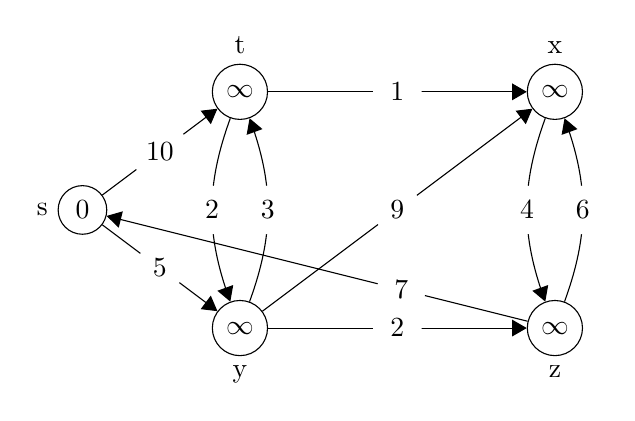
\begin{tikzpicture}[x=20mm, y=15mm]
	\node [circle, draw] (s) [label=left:{s}] at (0,0) {$0$};
	\node [circle, draw] (t) [label=above:{t}] at (1,1) {$\infty$};
	\node [circle, draw] (x) [label=above:{x}] at (3,1) {$\infty$};
	\node [circle, draw] (y) [label=below:{y}] at (1,-1) {$\infty$};
	\node [circle, draw] (z) [label=below:{z}] at (3,-1) {$\infty$};
	\draw[-triangle 60] (s) to node[circle, fill=white, midway]{10} (t);
	\draw[-triangle 60] (s) to node[circle, fill=white, midway]{5} (y);
	\draw[-triangle 60] (t) to node[circle, fill=white, midway]{1} (x);
	\draw[bend right=20, -triangle 60] (t) to node[circle, fill=white, midway]{2} (y);
	\draw[bend right=20, -triangle 60] (x) to node[circle, fill=white, midway]{4} (z);
	\draw[bend right=20, -triangle 60] (y) to node[circle, fill=white, midway]{3} (t);
	\draw[-triangle 60] (y) to node[circle, fill=white, midway]{9} (x);
	\draw[-triangle 60] (y) to node[circle, fill=white, midway]{2} (z);
	\draw[-triangle 60] (z) to node[circle, fill=white, pos=0.3]{7} (s);
	\draw[bend right=20, -triangle 60] (z) to node[circle, fill=white, midway]{6} (x);
\end{tikzpicture}

\subsubsection{Solution to Time Complexity Part}

The time complexity for Dijkstra's algorithm with the vertices stored in an array is $O(V^2)$.  If the vertices are stored in a binary min-heap, the time complexity is $O(E \lg V)$, which is faster if the graph is sparse.  If the graph is complete, $E = V(V-1)/2$, which would make the binary min-heap option $O(V^2 \lg V)$, worse than the array option.  

%%%%%
\subsubsection{Fall 2018 \#S1}
% Finished

	% F18 #S1
	The divide and conquer strategy (D\&C) has been used to solve problem efficiently to reduce the overall computational cost to certain types of problems.
	\begin{enumerate}[label=\alph*.]
		\item Which conditions have to be satisfied for D\&C to solve such problems successfully?  (Clearly state.)
		\item Suppose the size of a problem involved in D\&C is $n=2^k$.  Let the cost in dividing the problems into an equal size is constant and the time to combine solutions to sub-problems is linear.  Write the recurrence relations and then find the tight bound in solving such problems using D\&C.  
	\end{enumerate}
	
\subsubsection{Solution} \

Divide and conquer should be used (instead of dynamic programming) when the subproblems will not be solved only once.  

\begin{enumerate}[label=\alph*.]
\item The steps for divide and conquer are:

\begin{description}
	\item [Divide] the problem into subproblems.
	\item [Conquer] by recursively solving the subproblems. 
	\item [Combine] the solutions.  
\end{description}

\item
Let $T(n)$ be the running time of the algorithm for a problem of size $n$.  

Let $a$ be the (small) size of the problem for which the solution time is constant.  

Let $d$ be the constant cost of dividing the problems.  

Let $cn$ be the linear cost of combining the solutions to the subproblems.  

$$T(n) = 
\begin{cases}
	\Theta(1) & \text{if } n \le a \cr
	2 T \left( \frac{n}{2} \right) + d + cn & \text{otherwise} \cr
\end{cases}
$$

\begin{align*}
	T(n) &= 2 T \left( \frac{n}{2} \right) + d + cn\cr
	&= 2 \left[ 2T\left( \frac{n}{4} \right) + d + c\frac{n}{2} \right] + d + cn = 4T\left( \frac{n}{4} \right) + 3d + 2cn \cr
	&= 4 \left[ 2T\left( \frac{n}{8} \right) + d + c \frac{n}{4} \right] + 3d + 2cn = 8T\left( \frac{n}{8} \right) + 7d + 3cn  \cr
	&= \cdots = 2^k T \left( \frac{n}{2^k} \right) + (2^k-1)d + kcn \cr
	& \text{Terminates when } n = 2^k \iff k = \lg n. \cr
	&= (n-1)d + c n\lg n \cr
	&= \Theta(n \lg n) \cr
\end{align*}

\end{enumerate}

%%%%%	
\subsubsection{Fall 2018 \$S2}	
% Finished
	% F18 #S2
	\begin{enumerate}[label=\alph*.]
		\item What is the lower bound for comparisons based sorting algorithm? (Outline the justification of your answer.)
		\item What is the strategy behind greedy algorithm?
	\end{enumerate}
	
\subsubsection{Solution}

\begin{enumerate}[label=\alph*.]
	\item The lower bound (in the worst case) to sort $n$ elements by any comparison sort is $\Omega ( n \lg n )$, because it has to make that many comparisons.  
	\item The strategy behind a greedy algorithm is to find optimal solutions to subproblems, and build those together into an optimal solution to the original problem.  In order to work the problem must have the greedy choice property, that choosing locally optimal solutions leads to a globally optimal solution.  
\end{enumerate}

%%%%%
\subsubsection{Fall 2018 \#S3}	
% Finished. 
	% F18 #S3
	Find the tight bounds (by deriving their upper and lower bounds) of the following expressions.
	\begin{enumerate}[label=\alph*.]
		\item $\displaystyle T(n) = 2 \cdot T \left( \frac{n}{8} \right) + n^{\frac{1}{3}}$
		
		\vskip 6pt
		
		\item $T(n) = \log(n!)$
	\end{enumerate}
	
\subsubsection{Solutions}

\begin{enumerate}[label=\alph*.]

\item 
\begin{align*}
	 T(n) &= 2T\left(\frac{n}{8} \right) + n^{1/3} \cr
	 T\left( \frac{n}{8} \right) &= 2T\left(\frac{n}{8^2} \right) + \left(\frac{n}{8}\right)^{1/3} \cr
	 T\left( \frac{n}{8^2} \right) &= 2T\left(\frac{n}{8^3} \right) + \left(\frac{n}{8^2}\right)^{1/3} \cr
	 &\vdots \cr	 
	 T(n) &= 2T\left(\frac{n}{8} \right) + n^{1/3} \cr
	 &= 2\left(2T\left(\frac{n}{8^2} \right) + \left(\frac{n}{8}\right)^{1/3}  \right) + n^{1/3} = 4T\left(\frac{n}{8^2} \right) + 2n^{1/3} \cr
	 &= 4 \left( 2T\left(\frac{n}{8^3} \right) + \left(\frac{n}{8^2}\right)^{1/3} \right) + 2n^{1/3} =  8T\left(\frac{n}{8^3} \right) + 3n^{1/3}\cr
	 &= \log_8 n \cdot n^{1/3}\cr
	 T(n) &= \Theta(\root 3 \of n \cdot \lg n) \cr
\end{align*}

Because we didn't use any inequalities, we get Big-$\Theta$.  

\item Upper bound:

\begin{align*}
	\log(n!) &= \log(1 \cdot 2 \cdot \cdots \cdot n) \cr
		&= \log 1 + \log 2 + \cdots + \log n \cr
		&\le \log n + \log n + \cdots + \log n \cr
		&= n \log n \cr
\end{align*}

So $\log(n!) = O(n \log n)$.  
	
Lower bound:

\begin{align*}
	\log(n!) &=\log(1 \cdot 2 \cdot \cdots \cdot \frac{n}{2} \cdot \cdots \cdot n) \cr
		&= \log 1 + \log 2 + \cdots + \log \frac{n}{2} + \cdots + \log n\cr
		&\ge \log \frac{n}{2} + \log \left( \frac{n}{2} + 1 \right) + \cdots + \log n \cr
		&\ge \log \frac{n}{2} + \log \frac{n}{2} + \cdots + \log \frac{n}{2} \cr
		&= \frac{n}{2} \log \frac{n}{2} \cr
		&= \frac{n}{2} ( \log n - \log 2) \cr
		&\ge \frac{1}{4} n \log n \text{\qquad for } n\ge 4 \cr
\end{align*}

So $\log(n!) = \Omega(n \log n)$.  

Since $\log(n!) = \Omega(n \log n)$ and $\log(n!) = O(n \log n)$, therefore $\log(n!) = \Theta(n \log n)$.  

\end{enumerate}
	
%%%%%
\subsubsection{Fall 2018 \#L4}
% Finished
	%  F18 #L4
	The Dijkstra's algorithm (DS) solves the single-source shortest-path problem in a weighted graph $G = (V,E)$ without negative weighted edges or cycles, by edge relaxation at one vertex at a time until all vertices are examined.  Given the graph $G$ below, follow DS to find the shortest paths from vertex $v_1$ to all other vertices, with all predecessor edges shaded and estimated distance values from $v_1$ to all vertices provided at the end.  Also list the sequence of vertices at which relaxation takes place.  
	
	What is the time complexity of DS for a general graph $G = (V,E)$ when candidate vertices are kept in an array?
	
\hfil	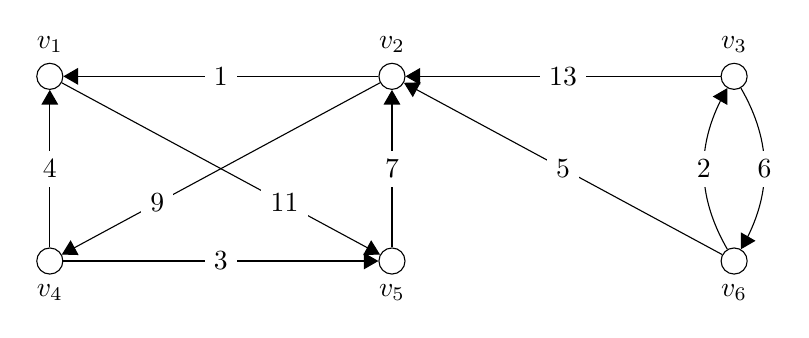
\begin{tikzpicture}[node distance = 2cm and 4cm]
		\node [circle, draw, label=above:$v_1$] (v1) {};
		\node [circle, draw, label=above:$v_2$, right=of v1] (v2) {};
		\node [circle, draw, label=above:$v_3$, right=of v2] (v3) {};
		\node [circle, draw, label=below:$v_4$, below= of v1] (v4) {};
		\node [circle, draw, label=below:$v_5$, right=of v4] (v5) {};
		\node [circle, draw, label=below:$v_6$, right=of v5] (v6) {};
		\foreach \from/\to/\label in {v2/v1/1, v3/v2/13, v4/v1/4, v4/v5/3, v5/v2/7, v6/v2/5}{
			\draw [-triangle 60] (\from) -- (\to) node [midway, rectangle, fill=white] {\label};
		}
		\foreach \from/\to/\label in {v1/v5/11, v2/v4/9}{
			\draw [-triangle 60] (\from) -- (\to) node [pos=0.7, rectangle, fill=white] {\label};
		}
		\foreach \from/\to/\label in {v3/v6/6, v6/v3/2}{
			\path [-triangle 60] (\from) edge [bend left] node [midway, rectangle, fill=white] {\label} (\to);
		}
		\foreach \from/\to/\label in {}{
			\draw [triangle 60-triangle 60] (\from) -- (\to) node [midway, rectangle, fill=white] {\label};
		}
 	\end{tikzpicture}
	
\subsubsection{Solution to Time Complexity Part}

The time complexity of Dijkstra's algorithm, if the candidate vertices are kept in an array, is $O(V^2)$.  If the candidate vertices are kept in a binary min-heap, then the time complexity is $O(E\lg V)$, which is worse if the graph is dense or complete, but better if the graph is sparse.  

%%%%%
\subsubsection{Spring 2018 \#S1}
% Finished

	% S18 #S1
	A problem with size $n$ follows a typical divide-and-conquer approach to have its time complexity of
	$$T(n) = T\left(\frac{n}{4} \right) + T \left( \frac{3n}{4} \right) + c \cdot n$$
	Solve $T(n)$.  (Show your work.)

\subsubsection{Solution}

\begin{align*}
	T(n) &= T\left(\frac{n}{4} \right) + T \left( \frac{3n}{4} \right) + c \cdot n \cr
		&= \left[ T\left(\frac{n}{16} \right) + T \left( \frac{3n}{16} \right) + \frac{cn}{4}\right] 
		+ \left[ T\left(\frac{3n}{16} \right) + T \left( \frac{9n}{16} \right) + \frac{3cn}{4}\right]  + cn \cr
		&= T\left(\frac{n}{4^2} \right) + 2T\left(\frac{3n}{4^2} \right) + T\left(\frac{3^2}{4^2}n \right) + 2cn \cr
		& \text{The recursion terminates when }\left( \frac{3}{4} \right) ^k n = 1 \text{ in step } k = \log_{4/3}n \cr
		T(n) &= (\log_{4/3} n )( c )( n )\cr
		T(n) &= O(n \log n) \cr
\end{align*}


%%%%%
\subsubsection{Spring 2018 \#S4}
% Finished

	% S18 #S4
	The Dijkstra's algorithm (DS) solves the single-source shortest-path problem in a weighted graph $G = (V,E)$ without negative weighted edges or cycles, by edge relaxation at one vertex at a time until all vertices are examined.  Given the graph $G$ below, follow DS to find the shortest paths from vertex $v_1$ to all other vertices, with all predecessor edges shaded and estimated distance values from $v_1$ to all vertices provided at the end.  Also list the sequence of vertices at which relaxation takes place.  
	
	What is the time complexity of DS for a general graph $G = (V,E)$ when candidate vertices are kept in an array?
	
\hfil	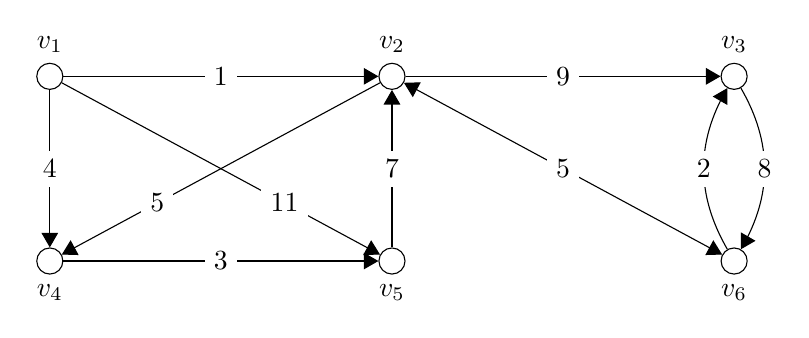
\begin{tikzpicture}[node distance = 2cm and 4cm]
		\node [circle, draw, label=above:$v_1$] (v1) {};
		\node [circle, draw, label=above:$v_2$, right=of v1] (v2) {};
		\node [circle, draw, label=above:$v_3$, right=of v2] (v3) {};
		\node [circle, draw, label=below:$v_4$, below= of v1] (v4) {};
		\node [circle, draw, label=below:$v_5$, right=of v4] (v5) {};
		\node [circle, draw, label=below:$v_6$, right=of v5] (v6) {};
		\foreach \from/\to/\label in {v1/v2/1, v1/v4/4, v2/v3/9, v4/v5/3, v5/v2/7}{
			\draw [-triangle 60] (\from) -- (\to) node [midway, rectangle, fill=white] {\label};
		}
		\foreach \from/\to/\label in {v1/v5/11, v2/v4/5}{
			\draw [-triangle 60] (\from) -- (\to) node [pos=0.7, rectangle, fill=white] {\label};
		}
		\foreach \from/\to/\label in {v3/v6/8, v6/v3/2}{
			\path [-triangle 60] (\from) edge [bend left] node [midway, rectangle, fill=white] {\label} (\to);
		}
		\foreach \from/\to/\label in {v2/v6/5}{
			\draw [triangle 60-triangle 60] (\from) -- (\to) node [midway, rectangle, fill=white] {\label};
		}
 	\end{tikzpicture}
	
\subsubsection{Solution to the Time Complexity Part}

When the vertices are kept in an array, the time complexity of Dijkstra's algorithm is $O(V^2)$.  When the vertices are kept in a binary min-heap, the time complexity is $O(E \lg V)$.  In a complete graph, $E = V(V-1)/2$, so for a complete (or even dense) graph, the array is faster, but for a sparse graph, the binary min-heap is faster.  

%%%%%
\subsubsection{Spring 2018 \#L3}
% Finished

	% S18 #L3
	\begin{enumerate}[label=\alph*.]
		\item To what extent the asymptotic upper bound and lower bound provide insight on running time of an algorithm.
		\item Compare and contrast asymptotic tight bound to the average running time of an algorithm.
		\item Consider the pseudo code of an algorithm given below.  
		\begin{enumerate}
			\item What the value $K$ in line 4 denote?
			\item What the value $m$ in line 8 denote?
			\item When the algorithm terminates, what does the value $m+K$ in line 9 denote?
			\item Find the asymptotic tight bound of Algorithm Test below.
		\end{enumerate}
	\end{enumerate}
	
	\verb|AlgorithmTest(n)|
	
	\begin{lstlisting}[mathescape=True, numbers=left]
$K=0$
for $i=1$ to $n$
	for $j=1$ to $i$
		$K = K+1$
$m=0$
for $i=1$ to $n-1$
	for $j=i+1$ to $n$
		$m = m+1$
return $(m+K)$
	\end{lstlisting}

\subsubsection{Solution}

\begin{enumerate}[label=\alph*.]
	\item The asymptotic lower bound gives the order of magnitude of the best-case running time of an algorithm for sufficiently large input size; for instance, the time to run a sorting algorithm on a list that is already sorted.  The asymptotic upper bound gives the worst-case run time.  
	
	The bounds do not give the actual run time, because there is a (perhaps unknown) constant not given.  The bounds show how the run time increases with input size.  If the upper bound of algorithm $A$ is of lower order than the lower bound of algorithm $B$, there is an input size for which $A$ is always faster than $B$, but the input size may be larger than an actual application.  
	
	\item There are some actual applications for which we have algorithms with an asymptotic tight bound, like multiplication of dense square matrices of uniform data types (like double-precision floats).  For matrices of size $n \times n$, the algorithm has asymptotic tight bound $\Theta(n^3)$, meaning that, for sufficiently large $n$, there exist constants $c_1$ and $c_2$ such that the algorithm takes between $c_1n^3$ and $c_2n^3$ units of time, but $c_1$ and $c_2$ are not given, and in practice depend on everything from the hardware to the weather.  The asymptotic tight bound also makes the heroic assumption that the data needed is always in the registers, when in fact, for sufficiently large $n$, the data may not fit in cache or even in main memory.  The asymptotic tight bound is not very useful in predicting average running time of a particular instance, but is useful in comparing algorithms and understanding how the average running time will increase with the size of the input.  
	
	\item 
	\begin{enumerate}
		\item The value of $K$ denotes the arithmetic series $1 + 2 + 3 + \cdots + n = (n)(n+1)/2$.
		\item The value of $m$ denotes the arithmetic series $(n-1) + (n-2) + \cdots + 2 + 1 = (n-1)(n)/2$.  
		\item The value of $m+K$ is $n^2$.  
		\item The asymptotic tight bound is $\Theta(n^2)$, which is the number of additions and the number of calls to the inner loops.  The number of calls to the outer loops is $O(n)$, and there's some constant overhead. 
	\end{enumerate}
\end{enumerate}

%%%%%
\subsubsection{Spring 2017 \#S1}
% Finished
	% S17 #S1
	\begin{enumerate}[label=\alph*.]
		\item Define height balanced binary tree.
		\item Write a pseudo code to determine whether a tree is height balanced?
		\item Obtain the tight bound of your algorithm.
	\end{enumerate}

\subsubsection{Solutions}

\begin{enumerate}[label=\alph*.]
	\item A height balanced binary tree is a binary tree such that, for each node $x$, the heights of the left and right subtrees of $x$ differ by at most 1.  Alternately, the depths of the leaves differ by no more than 1.  
	\item Run BFS from the root.  First use the results to find the largest distance from the root to another node.   This largest distance will be the height of the tree, $h$.  Use the BFS results a second time to count the nodes whose depth (distance from the root) is $h-1$.  Iff that number of nodes is $2^{h-1}$, then the tree is height balanced.  For example, if the 
	\item The time complexity of BFS is $O(V+E)$.  In a binary tree, $E = V-1$ and $V \le 2^{h+1}-1 < 2 \cdot 2^h$, so the time complexity of BFS on a binary tree is $O(V) = O(2^h)$.  It would be nice if the time complexity for BFS on a binary tree were less than for a general tree, but to get the depths of the leaf nodes we have to visit every node, and there are $V$ of them, so we can't hope for time complexity less than linear in $V$.  Tracking the maximum distance and counting the number of nodes with depth $n-1$ are at worst linear in $V$, so the time complexity of the algorithm is $\Theta(V) = \Theta(2^h)$.  
\end{enumerate}

%%%%%
\subsubsection{Spring 2017 \#S2}
% Finished
	% S17 #S2
	Suppose you have keys of $N$ objects stored in an array in the ascending order of key values.  Also assume that there is duplicate entry in the key.  
	\begin{enumerate}[label=\alph*.]
		\item Describe an efficient algorithm with the pseudo code that helps you to search for the object given the key. (The algorithm must return null value if the key is not in the array.) 
		\item Obtain the tight upper bound for your algorithm.
	\end{enumerate}
	
\subsubsection{Solutions}

\begin{enumerate}[label=\alph*.]
	\item Take a divide-and-conquer approach, bracket-and-halving.
	
	Let 
	$N$ be the number of objects, 
	$k$ the key of the object we seek, and
	$A$ the array.
	
	Assume that all division truncates.

	Let $a=1$ and $c=N$.  
	
	At each step, 
	
	\begin{enumerate}[label=\arabic*.]
		\item $b = (a+c)/2$
		\item if $A[b]==k$, return $b$
		\item if $a==c$, return NULL
		\item if $A[b] < k$, then $a=b+1$
		\item if $k < A[b]$, then $c = b-1$
	\end{enumerate}
	
	\item The tight upper bound for the algorithm is $O(\lg N)$.  
		
\end{enumerate}

%%%%%
\subsubsection{Spring 2017 \#S4}
% Finished
	% S17 #S4
	Find the tight for the recurrence relation below without using the master theorem (show all the steps):
	$$T(n) = T(n/2) + n$$
	
\begin{align*}
	T(n) &= T\left( \frac{n}{2} \right) + n \cr
	&= \left[ T\left( \frac{n}{4} \right) + \frac{n}{2} \right] + n  = T \left( \frac{n}{4} \right) + \frac{3}{2} n\cr
	&= \left[ T \left( \frac{n}{8} \right) + \frac{n}{4} \right] + \frac{3}{2}n = T \left( \frac{n}{8} \right) + \frac{7}{4}n \cr
	&= \cdots = T \left( \frac{n}{2^k} \right) + \frac{2^k-1}{2^{k-1}} n \cr
	& \qquad \frac{n}{2^k} = 1 \text{ when } k = \log_2 n \cr
	&= (\log_2 n) \left( \frac{2^{\log_2 n} - 1}{2^{\log_2 n - 1}} n \right) 
	= (\log_2 n) \left( \frac{n-1}{n/2} \right) n
	= (\log_2 n) (2)(n-1) \cr
	&= \Theta(n \log n) \cr
\end{align*}

%%%%%
\subsubsection{Fall 2016 \#S1}
% Finished
	% F16 #S1
	\begin{enumerate}
		\item Define an upper and the tight time bound of an algorithm.
		\item In which way the average time bound will add more value to the tight bound?
	\end{enumerate}
	
\subsubsection{Solutions}

\begin{enumerate}
	\item The time bounds are a function of the size of the inputs into an algorithm, such that the running time should be proportional to the value of the function for the input size.  Because they are proportional, we can ignore constants.  The upper bound gives the worst-case scenario, and the lower bound gives the best-case.  If the ratio of the upper to the lower bound does not depend on the input size, then the tight bound exists.  
	\item For a given input size, the running time is proportional to the tight bound, but the constant of proportionality is unknown.  The average time bound may give more information, equivalent to an estimate of the constant.  
\end{enumerate}
	
%%%%%	
\subsubsection{Fall 2016 \#S2}
% Not finished
	% F16 #S2	
	\begin{enumerate}
		\item Briefly describe a quick sort algorithm for sorting objects in an ascending order of their keys.
		\item What is the best and worst case time complexity of quick sort and the reason for such complexity?
	\end{enumerate}
	
\subsubsection{Solution}

\begin{enumerate}
	\item
	
	\item Worst case:  $\Theta (n^2)$.  
\end{enumerate}
	
%%%%%
\subsubsection{Fall 2016 \#S3}
% Finished
	% F16 #S3
	Find the tight [time bound, time complexity?] for the recurrence relations without using the master theorem. 
	\begin{enumerate}
		\item $T(n) = T(n-2) + 2 \lg(n)$
		\item $T(n) = T(\sqrt{n}) + \lg(n)$
	\end{enumerate}
	
\subsubsection{Solution}
	
\begin{enumerate}
	\item	$T(n) = T(n-2) + 2 \lg n$
	
\begin{align*}
	T(n) &= T(n-2) + 2 \lg (n) \cr
	&= \left[ T(n-4) + 2 \lg(n-2) \right] + 2 \lg (n)
	= T(n-4) + 2 \lg[(n)(n-2)] \cr
	&= \left[ T(n-6) + 2\lg(n-4) \right] + 2\lg[(n)(n-2)] 
	= T(n-6) + 2\lg[(n)(n-2)(n-4)] \cr
	&= \cdots = T(0) + 2 \lg[(n)(n-2)(n-4) \cdots (4)(2)] \cr
 	T(n) &= 2 \lg (n) + 2 \lg(n-2) + \cdots + 2 \lg 2 \cr
\end{align*}

Upper bound
\begin{align*}
 	T(n) &= 2 \lg (n) + 2 \lg(n-2) + \cdots + 2 \lg 2 \cr
	&\le 2 \lg n + 2 \lg n + \cdots + 2 \lg n \cr
	&= 2 \frac{n}{2} \lg n \cr
	&= n \lg n \cr
	T(n) &= O(n \lg n) \cr
\end{align*}

Lower bound
\begin{align*}
	T(n) &= 2 \lg (n) + 2 \lg(n-2) + \cdots + 2\lg (n/2) + 2 \lg (n/2 - 2) + \cdots + 2 \lg 2 \cr
	&\ge 2 \lg (n) + 2 \lg(n-2) + \cdots + 2\lg (n/2) \cr
	&= 2 \lg n + 2 \lg n + \cdots 2 \lg n \cr
	&\ge 2 \frac{n}{4} \lg n = \frac{1}{2} n \lg n \cr
	T(n) &= \Omega(n \lg n) \cr
\end{align*}

Since $T(n) = O(n \lg n)$ and $T(n) = \Omega(n \lg n)$, $T(n) = \Theta(n \lg n)$.  	

	\item $T(n) = T(\sqrt{n}) + \lg n$

\begin{align*}
	T(n) &= T\left( n^\frac{1}{2} \right) + \lg \left( n \right) \cr
	&= \left[ T\left( n^\frac{1}{4} \right) + \lg \left( n^\frac{1}{2} \right) \right] + \lg \left( n \right) = T\left( n^\frac{1}{4} \right) + \lg n + \frac{1}{2} \lg n \cr
	&= 	T \left( n^\frac{1}{2^k} \right) + \lg n + \frac{1}{2}\lg n + \cdots + \frac{1}{2^{k-1}} \lg n \cr
	&= T\left( n^\frac{1}{2^k} \right) +  \left( 1 + \frac{1}{2} + \cdots + \frac{1}{2^{k-1}} \right) \lg n \cr
	&= T\left( n^\frac{1}{2^k} \right) +  \left( \frac{2^k - 1}{2^{k-1}}  \right) \lg n\cr
\end{align*}

This problem is different from the others in that we can't directly find how many steps we'd need to take to get the argument of $T$ to be 1, because that only happens with rounding, but we can find where the argument is 2. 

Solve for $k$ when the argument is 2, as an approximation of how many steps it takes to get to an argument of 1.  

Alternately, rather that 2 we could use any constant, which would become the base of the log in the solution, so the solution would be within that constant of the number of steps.  

\begin{align*}
	n^\frac{1}{2^k} &= 2 \cr
	\frac{1}{2^k} \log_2 n &= 1 \cr
	\log_2 n &= 2^k \cr
	\log_2 (\log_2 n) &= k \cr
\end{align*}	

\begin{align*}
	T(n) &= T\left( n^\frac{1}{2^k} \right) +  \left( \frac{2^k - 1}{2^{k-1}}  \right) \lg n\cr
	&= T\left( 2 \right) +  \left( \frac{\log_2 n - 1}{\log_2 n)/2}  \right) \lg n\cr
	&= T\left( 2 \right) +  \left( \frac{\log_2 n - 1}{\log_2 n)/2}  \right) \lg n\cr
	&= T\left( 2 \right) +  2(\log_2 n - 1)\cr
	& \text{Because there was no inequality, we get $\Theta$.} \cr
	&= \Theta(\lg n) \cr
\end{align*}


	
\end{enumerate}
	
%%%%%
\subsubsection{Fall 2016 \#S5}	
% Not finished
	% F16 #S5
	Suppose there are $n$ clauses and $m$ variables (propositions) in a given $3-p$ sat problem.
	\begin{itemize}
		\item How many possible interpretations are there?
		\item Find the tight bound of checking for satisfiability of the $n$ clauses.  
	\end{itemize}
	
%%%%%
\subsubsection{Fall 2015 \#S1}
% Finished
	% #F15 S1
	Show that for arbitrary real constants $a$ and $b$ with $b>0$, we have $(n+a)^b = \Theta(n^b)$.
	
\subsubsection{Solution}
	
$f(n) = \Theta(g(n))$ iff there exist constants $c_1$, $c_2$, and $n_0$ such that for all $n\ge n_0$, $$0 \le c_1 g(n) \le f(n) \le c_2 g(n)$$

Show that there exist positive constants $c_1$, $c_2$, and $n_0$ such that, for all $n \ge n_0$, $$0 \le c_1 n^b \le (n+a)^b \le c_2 n^b$$

In the following calculations, assume $n \ge \max(-a,1)$ so that both $n$ and $n+a$ are positive.  Then because both sides of the inequality are positive and the logarithm is an increasing function, taking the log of both sides preserves the inequality.  

\begin{align*}
	c_1 n^b &\le (n+a)^b \cr
	\log(c_1 n^b) &\le \log \left( \left(n+a\right)^b\right) \cr
	\log c_1 + b \log n &\le b \log (n+a) \cr
	\log c_1 &\le b \log (n+a) - b\log n \cr
	\log c_1 &\le b \log \frac{n+a}{n} \cr
	c_1 &\le \left( \frac{n+a}{n} \right)^b \cr		
\end{align*}

Similarly for $c_2$, so $\displaystyle c_1 \le \left( \frac{n+a}{n} \right)^b \le c_2$.  

If $a\ge 0$, then $\frac{n+a}{n}$ decreases towards 1 as $n \to \infty$ and $\min \left( \frac{n+a}{n} \right)^b=1$.  

If, however, $a<0$, then $\displaystyle\frac{n+a}{n}$ increases towards 1 as $n \to \infty$, and its min value in the range $[n_0, \infty)$ is $\displaystyle\frac{n_0+a}{n_0}$.  

I will choose $n_0 = |a|+1$ so that $\displaystyle\min \left(\frac{n_0+a}{n_0} \right) = \frac{1}{|a|+1}$ and $\displaystyle\max\left(\frac{n_0+a}{n_0} \right) = \frac{2|a|+1}{|a|+1} < 2$

Let $n_0 = |a|+1$,  $\displaystyle c_1 = \left(\frac{1}{|a|+1}\right)^b$ and $\displaystyle c_2 = 2^b$.  

\

Then for all $n \ge n_0$, $0 \le c_1 n^b \le (n+a)^b \le c_2n^b$, so $(n+a)^b = \Theta (n^b)$.  

%%%%%
\subsubsection{Fall 2015 \#S2}	
% Finished
	% #F15 S2
	Use the recursion-tree technique to derive the tight lower and upper bounds of the recursion $T(n) = T(n/3) + T(2n/3) + cn$.
	
\

[Note that this exercise is the example on page 91.]

\subsubsection{Solution}

\begin{align*}
	T(n) &= T\left( \frac{1}{3} n \right) + T \left( \frac{2}{3} n \right) + cn \cr
	&= \left[ T\left( \frac{1}{9} n \right) + T \left( \frac{2}{9} n \right) + \frac{1}{3}cn\right] + \left[ T\left( \frac{2}{9} n \right) + T \left( \frac{4}{9} n \right) + \frac{2}{3}cn\right] + cn \cr
	&= T\left( \frac{1}{9} n \right) + 2T\left( \frac{2}{9} n \right) + T\left( \frac{4}{9} n \right) + 2cn \cr
	&= \left[ T\left( \frac{1}{27} n \right) + T \left( \frac{2}{27} n \right) + \frac{1}{9}cn\right] + 
	2\left[ T\left( \frac{2}{27} n \right) + T \left( \frac{4}{27} n \right) + \frac{2}{9}cn\right] + 
	\left[ T\left( \frac{4}{27} n \right) + T \left( \frac{8}{27} n \right) + \frac{4}{9}cn\right] + 2cn \cr	
	&= T\left( \frac{1}{27} n \right) + 2 T\left( \frac{2}{27} n \right) + 2T\left( \frac{4}{27} n \right) + T\left( \frac{8}{27} n \right) + 3cn \cr
	&= \cdots = T\left( \frac{1}{3^k} n \right) + 2T\left( \frac{2}{3^k} n \right) + 2T\left( \frac{2^2}{3^k} n \right) + \cdots + 2T\left( \frac{2^{k-1}}{3^k} n \right) +  T\left( \frac{2^k}{3^k} n \right) + kcn \cr
	& \text{Last step when } \frac{2^k}{3^k}n=1, \text{ which happens when } k = \log_{3/2}n \cr
	&= \log_{3/2}n \cdot c \cdot n \cr
	&= \Theta ( n \lg n) \cr
\end{align*}

%%%%%
\subsubsection{Fall 2015 \#L3}	
% Finished
	% F15 # L3
	In the following pseudo code, 
	\begin{enumerate}[label=\alph*.]
		\item Write the formula to determine the number of add operations at line 5 when the algorithm terminates.  
		\item What is the space complexity?
		\item Find the following time bounds of this algorithm:  Upper, lower, and tight. (Must show all the details of your work.)
	\end{enumerate}
	
	\
	
	\verb|Algorithm Count|
	
	\begin{lstlisting}[numbers=left, mathescape=true]
$Cnt = 0$
for $i=1$ to $n$ do {
	for $j = 1$ to $i^2$ do {
		for $k=1$ to $j$ do {
			$Cnt = Cnt + 1$
		}
	}
}
	\end{lstlisting}
	
	Note that I have corrected (?) line 3 from \ \verb|for j=i^2 to i do {|
	
	This question is weird.  
	
\subsubsection{Solution?}

\begin{align*}
	Cnt &= \sum_{i=1}^n \sum_{j=1}^{i^2} j \cr
		&= 1 + (1+2+3+4) + (1 + 2 + \cdots + 9) + \cdots + \frac{n^2(n^2+1)}{2} \cr
		&\le n \cdot \frac{n^2(n^2+1)}{2} \cr
		&\le n^5 \cr
\end{align*}

The number of add operations is the same as the value of $Cut$.  I've found a upper bound.  

%%%%%
\subsubsection{Spring 2015 \#S1}
% Finished
	% S15 #S1
	Briefly define upper, lower, and tight time bound of an algorithm.  How does an average time complexity related to any of these bounds?
	
\subsubsection{Solution}

See Fall 2016 \#S1.  
	
%%%%%
\subsubsection{Spring 2015 \#S2}
% Not finished
	% S15 \#S2
	In terms of run time efficiency, compare and contrast quick sort and merge sort.  What is the best and the worst case time complexity of the quick sort algorithm?  Also state under what conditions one may expect these two extreme cases.
	
%%%%%
\subsubsection{Spring 2015 \#S3}
% Finished
	% S15 #S3
	Find the tight bounds of the following sums.  
	\begin{enumerate}
		\item $\displaystyle \sum_{i=1}^n i^3 a^i$ where $a$ is a constant greater than 1
		\item $\displaystyle \sum_{i=1}^n \log (i^3)$ 
	\end{enumerate}
	
\subsubsection{Solution}

\begin{enumerate}
	\item No idea.  
	\item 
Upper bound:
\begin{align*}
	\sum_{i=1}^n \log(i^3) &= 3 \sum_{i=1}^n \log(i) \cr
		&= 3 ( \log 1 + \log 2 + \cdots + \log n) \cr
		&= 3\log(1 \cdot 2 \cdot \cdots \cdot n) \cr
		&= 3 \log(n!) \cr
		&\le 3 \log(n^n) \cr
		&= 3n \log n \cr
		\sum_{i=1}^n \log(i^3) &= O(n \log n) \cr
\end{align*}

Lower bound:  
\begin{align*}
	\sum_{i=1}^n \log(i^3) &= 3 \sum_{i=1}^n \log(i) \cr
		&= 3 ( \log 1 + \log 2 + \cdots + \log(n/2) + \cdots + \log n) \cr
		&\ge 3(\log(n/2) + \log(n/2+1) + \cdots + \log n) \cr
		&\ge 3(\log(n/2) + \log(n/2) + \cdots + \log(n/2)) \cr
		&= 3(n/2)(\log(n/2)) \cr
		&= \frac{3n}{2}(\log n - \log 2) \cr
		&\ge \frac{3n}{4}\log n \text{\qquad for } n\ge 4 \cr
		&= \frac{3}{4} n \log n \cr
	\sum_{i=1}^n \log(i^3) &= \Omega(n \log n) \cr
\end{align*}

Since $\displaystyle \sum_{i=1}^n \log(i^3) = \Omega(n \log n)$ and 
$\displaystyle \sum_{i=1}^n \log(i^3) = O(n \log n)$, 
$\displaystyle \sum_{i=1}^n \log(i^3) = \Theta(n \log n)$.
\end{enumerate}




% Search
\chapter{Data Structures and Search Algorithms}
%%%%%%%%%%%%%%%%%%	
\section{Balanced Search Tree} (\S 18.1, page 488) A B-tree $T$ is a rooted tree (whose root is $T.root$) having the following properties.  
	\begin{enumerate}
		\item Every node $x$ has the following attributes.
		\begin{enumerate}
			\item $x.n$, the number of keys currently stored in node $x$, 
			\item The $x.n$ keys themselves, $x.key_1, x.key_2, \dots, x.key_{x.n}$, stored in nondecreasing order, so that $x.key_1 \le x.key_2 \le \cdots \le x.key_{x.n}$.
			\item $x.leaf$, a boolean value that is \verb|True| if $x$ is a leaf and \verb|False| if $x$ is an internal node.  
		\end{enumerate}
		\item Each internal node $x$ also contains $x.n+1$ pointers, $x.c_1, x.c_2, \dots, x.c_{x.n+1}$ to its children.  Leaf nodes have no children, and so their $c_i$ attributes are undefined.  
		\item The keys $x.key_i$ separate the ranges of keys stored in each subtree.  If $k_i$ is any key stored in the subtree with root $x.c_i$, then 
		$$k_1 \le x.key_1 \le k_2 \le x.key_2 \le \cdots \le x.key_{x.n} \le k_{x.n+1}$$
		\item All leaves have the same depth, which is the tree's height, $h$.  
		\item Nodes have lower and upper bounds on the number of keys they can contain.  We express these bounds in terms of a fixed integer $t \ge 2$ called the {\it minimum degree} of the B-tree.  
		\begin{enumerate}
			\item Every node other than the root must have at least $t-1$ keys.  Every internal node other than the root thus has at least $t$ children.  If the tree is nonempty, the root must have a least one key.  
			\item Every node may contain at most $2t-1$ keys.  Therefore, an internal node may have at most $2t$ children.  We say that a node is {\it full} if it contains exactly $2t-1$ keys.  
		\end{enumerate}
	\end{enumerate} 
	\index{Balanced Search Tree!Definition!\S 18.0 - 18.3}
	
\subsection{Method for Inserting and Deleting a Key}

In a B-tree (Balanced binary tree) with minimum degree $t$, each node other than the root must have at least $t-1$ keys, and each node including the root must have at most $2t-1$ keys.  When we delete or insert a key, we don't know up front the node from which we're going to insert or delete the key, and we want to make just one pass from root to leaf, so we're going to adjust appropriately as we go.  

When deleting a key, when passing from the root to a leaf, if a node and its children together can be merged (contain no more than $2k-1$ keys), merge them.

When inserting a key, when passing from the root to a leaf, if a node has the maximum ($2k-1$) number of keys, split it.  
	
%%%%%%%%%%
\subsection{Old Exam Questions}

Note:  Why do they introduce keys with subscripts, instead of just using $A$ through $Z$?  Twenty-six keys is plenty for these exercises.  

%%%%%
\subsubsection{S19 \#L1}
	
	 Given a B-tree with the minimum degree of $t=3$ below, show the results after (i) deleting $B$, (ii) followed by inserting $M$, (iii) then followed by deleting $T$, and then inserting $M_t$ for $M<M_t<N$
	
	\index{Balanced Search Tree!S19 \#L1}
	
\
	
\hfil	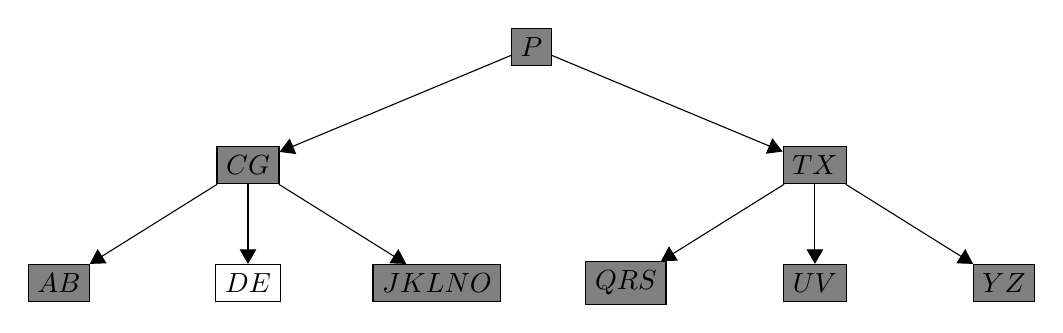
\begin{tikzpicture}[x=12mm, y=15mm]
		\node [rectangle, draw, fill=gray] (0) at (0,0) {$P$};
		\node [rectangle, draw, fill=gray] (1) at (-3,-1) {$C G$};
		\node [rectangle, draw, fill=gray] (2) at (3,-1) {$T X$};
		\node [rectangle, draw, fill=gray] (3) at (-5,-2) {$A B$};
		\node [rectangle, draw, fill=white] (4) at (-3,-2) {$D E$};
		\node [rectangle, draw, fill=gray] (5) at (-1,-2) {$JKL NO$};
		\node [rectangle, draw, fill=gray] (6) at (1,-2) {$QRS$};
		\node [rectangle, draw, fill=gray] (7) at (3,-2) {$UV$};
		\node [rectangle, draw, fill=gray] (8) at (5,-2) {$YZ$};
		\draw [-triangle 60] (0) -- (1); 
		\draw [-triangle 60] (0) -- (2); 
		\draw [-triangle 60] (1) -- (3); 
		\draw [-triangle 60] (1) -- (4); 
		\draw [-triangle 60] (1) -- (5); 
		\draw [-triangle 60] (2) -- (6); 
		\draw [-triangle 60] (2) -- (7); 
		\draw [-triangle 60] (2) -- (8); 
	\end{tikzpicture}
	
	Note:  The different shading of the nodes is not relevant.  They copied this from some book exercise where the node color indicated some step in a process that is not described here.  
	
\subsubsection{Solution}

{\bf Original Tree}

\
	
\hfil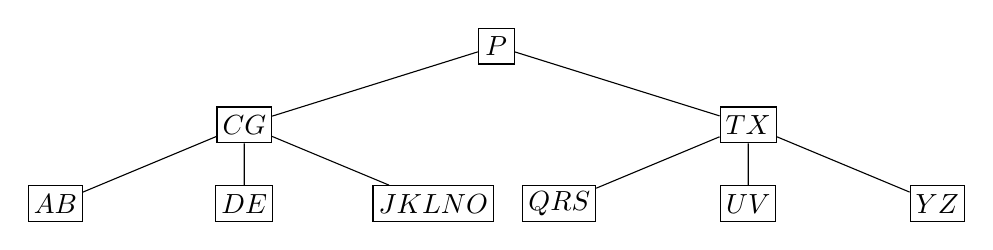
\begin{tikzpicture}[
	level 1/.style={level distance=10mm,sibling distance=64mm},
	level 2/.style={level distance=10mm,sibling distance=24mm},
	level 3/.style={level distance=10mm,sibling distance=16mm},
	inner sep=2pt,every node/.style={draw,rectangle,minimum size=3ex}]
  \node {$P$}
  child {node {$CG$}
  	child {node {$AB$}}
	child {node {$DE$}}
	child {node {$JKLNO$}}
  }
  child {node {$TX$}
  	child {node {$QRS$}}
	child {node {$UV$}}
	child {node {$YZ$}}
  };
\end{tikzpicture}

\

{\bf i. Delete $B$.}

Instructions on ``Deleteing a key from a B-tree,'' part 3.  Starting at $x = root$, ``If the key $k$ is not present in internal node $x$, determine the root $x.c_i$ of the appropriate subtree that must contain $k$, if $k$ is in the tree at all.''  Since $B<P$, we must go to the left to $x.c_1 = CG$.    

``If $x.c_i$ has only $t-1$ keys, execute step 3a or 3b as necessary to guarantee that we descend to a node containing at least $t$ keys.  Then finish by recursing on the appropriate child of $x$.  

It is true that $x.c_1 = CG$ has only $t-1=2$ keys.  

``3a.  If $x.c_i$ has only $t-1$ keys but has an immediate sibling with at least $t$ keys,....''  Not true, since the only sibling of $CG$ is $TX$, which also has only $2<t$ keys.  

``3b.  If  $x.c_i$ and both of $x.c_i$'s immediate siblings have $t-1$ keys, merge $x.c_i$ with one sibling, which involves moving a key from $x$ down into the new merged node to become the median key for that node.''

We need to merge $CG$ and $TX$, moving $P$ down into the new merged node to become the median key for that node.  



  First merge $P$, $CG$, and $TX$.  

\
	
\hfil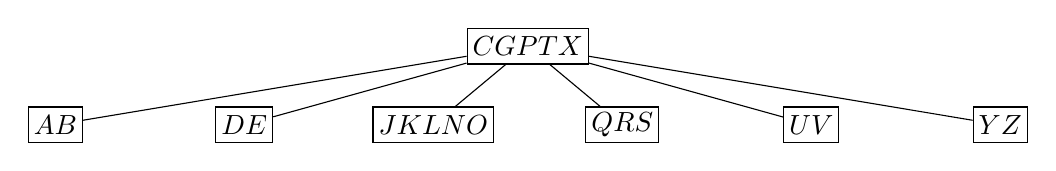
\begin{tikzpicture}[
	level 1/.style={level distance=10mm,sibling distance=24mm},
	level 2/.style={level distance=10mm,sibling distance=16mm},
	level 3/.style={level distance=10mm,sibling distance=16mm},
	inner sep=2pt,every node/.style={draw,rectangle,minimum size=3ex}]
  \node {$CGPTX$}
	child {node {$AB$}}
	child {node {$DE$}}
	child {node {$JKLNO$}}
  	child {node {$QRS$}}
	child {node {$UV$}}
	child {node {$YZ$}}
;
\end{tikzpicture}

\

Recurse.  We are at node $CGPTX$.

``3.  If the key $k$ is not present in internal node $x$, determine the root $x.c_i$ of the appropriate subtree that must contain $k$, if $k$ is in the tree at all.''  The key $B$ must be in the subtree rooted at $x.c_1 = AB$.  

``If $x.c_1$ has only $t-1$ keys, execute step 3a or 3b as necessary to guarantee that we descend to a node containing at least $t$ keys.''  It is true that $x.c_1$ has only $t-1=2$ keys.  

``3a.  If $x.c_i$ has only $t-1$ keys but has an immediate sibling with at least $t$ keys...''  Nope.  

``3b.  If $x.c_i$ and both of $x.c_i$'s immediate siblings have $t-1$ keys, merge $x.c_i$ with one sibling, which involves moving a key from $x$ down into the new merged node to become the median key for that node.''

Merge $AB$ and $DE$, bringing down $C$.  

\

\hfil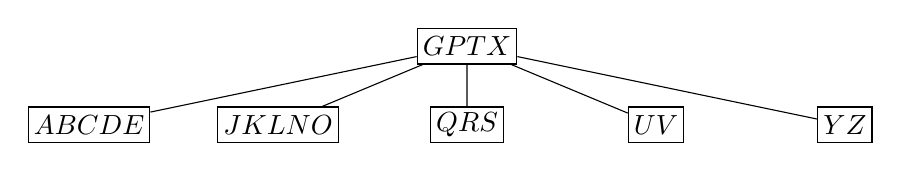
\begin{tikzpicture}[
	level 1/.style={level distance=10mm,sibling distance=24mm},
	level 2/.style={level distance=10mm,sibling distance=16mm},
	level 3/.style={level distance=10mm,sibling distance=16mm},
	inner sep=2pt,every node/.style={draw,rectangle,minimum size=3ex}]
  \node {$GPTX$}
	child {node {$ABCDE$}}
	child {node {$JKLNO$}}
  	child {node {$QRS$}}
	child {node {$UV$}}
	child {node {$YZ$}}
;
\end{tikzpicture}

\

Recurse.  We are at node $x=ABCDE$.  

``1.  If the key $k$ is in node $x$ and $x$ is a leaf, delete the key $k$ from $x$.''  

\

\hfil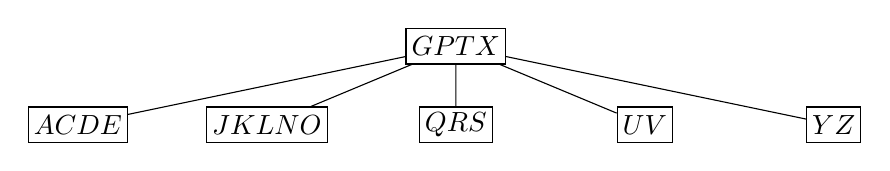
\begin{tikzpicture}[
	level 1/.style={level distance=10mm,sibling distance=24mm},
	level 2/.style={level distance=10mm,sibling distance=16mm},
	level 3/.style={level distance=10mm,sibling distance=16mm},
	inner sep=2pt,every node/.style={draw,rectangle,minimum size=3ex}]
  \node {$GPTX$}
	child {node {$ACDE$}}
	child {node {$JKLNO$}}
  	child {node {$QRS$}}
	child {node {$UV$}}
	child {node {$YZ$}}
;
\end{tikzpicture}

\


{\bf ii.  Insert $M$.}

It's going to go into $JKLNO$, but that would be too big, so split $JKLNO$ into $JK$ and $NO$, moving $L$ up into $GPTX$.  Then insert $M$ into $NO$.  

\

\hfil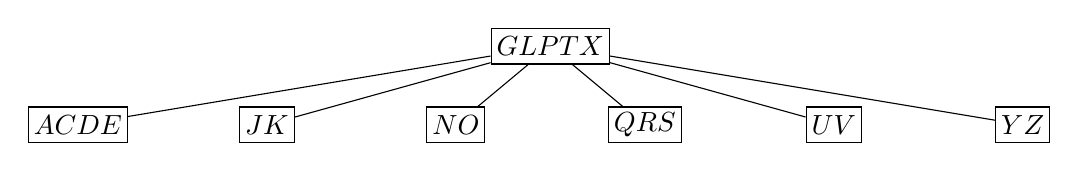
\begin{tikzpicture}[
	level 1/.style={level distance=10mm,sibling distance=24mm},
	level 2/.style={level distance=10mm,sibling distance=16mm},
	level 3/.style={level distance=10mm,sibling distance=16mm},
	inner sep=2pt,every node/.style={draw,rectangle,minimum size=3ex}]
  \node {$GLPTX$}
	child {node {$ACDE$}}
	child {node {$JK$}}
	child {node {$NO$}}
  	child {node {$QRS$}}
	child {node {$UV$}}
	child {node {$YZ$}}
;
\end{tikzpicture}


\

\hfil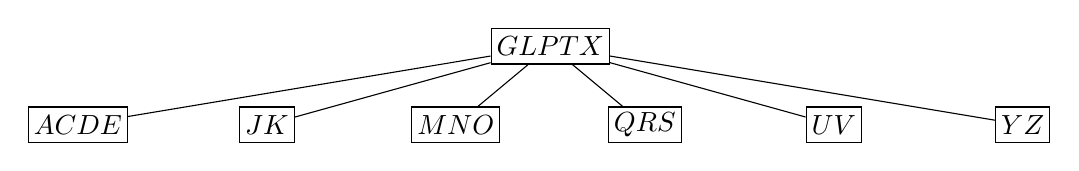
\begin{tikzpicture}[
	level 1/.style={level distance=10mm,sibling distance=24mm},
	level 2/.style={level distance=10mm,sibling distance=16mm},
	level 3/.style={level distance=10mm,sibling distance=16mm},
	inner sep=2pt,every node/.style={draw,rectangle,minimum size=3ex}]
  \node {$GLPTX$}
	child {node {$ACDE$}}
	child {node {$JK$}}
	child {node {$MNO$}}
  	child {node {$QRS$}}
	child {node {$UV$}}
	child {node {$YZ$}}
;
\end{tikzpicture}

\


{\bf iii.  Delete $T$.}  

``2.  If the key $k$ is in node $x$ and $x$ is an internal node, do the following:

a.  If the child $y$ that precedes $k$ in node $x$ has at least $t$ keys, then find the predecessor $k'$ of $k$ in the subtree rooted at $y$.  Recursively delete $k'$, and replace $k$ by $k'$ in $x$.''

In this case, if the key $T$ is in node $GLPTX$ and $GLPTS$ is an internal node, do the following:

a.  If the child $QRS$ that precedes $T$ in node $GLPTX$ has at least $t=3$ keys [which it does], then find the predecessor $S$ of $T$ in the subtree rooted at $QRS$.  Recursively delete $S$, and replace $T$ by $S$ in $GLPTX$.  

\

\hfil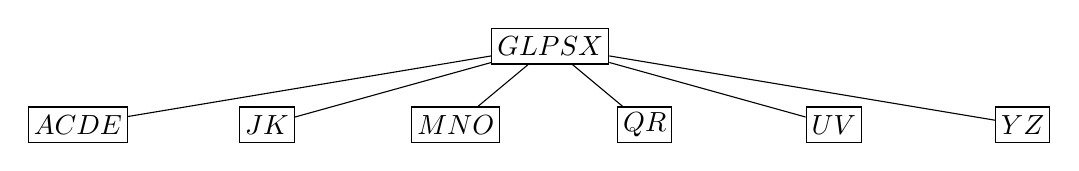
\begin{tikzpicture}[
	level 1/.style={level distance=10mm,sibling distance=24mm},
	level 2/.style={level distance=10mm,sibling distance=16mm},
	level 3/.style={level distance=10mm,sibling distance=16mm},
	inner sep=2pt,every node/.style={draw,rectangle,minimum size=3ex}]
  \node {$GLPSX$}
	child {node {$ACDE$}}
	child {node {$JK$}}
	child {node {$MNO$}}
  	child {node {$QR$}}
	child {node {$UV$}}
	child {node {$YZ$}}
;
\end{tikzpicture}

\



{\bf iv.  Insert $M_t$ for $M < M_t < N$.}  

The first thing to do is to split $GLPSX$.  

\

\hfil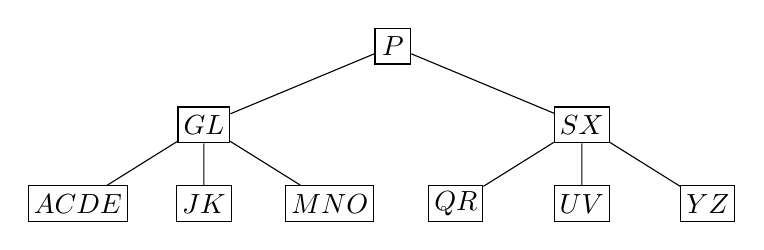
\begin{tikzpicture}[
	level 1/.style={level distance=10mm,sibling distance=48mm},
	level 2/.style={level distance=10mm,sibling distance=16mm},
	level 3/.style={level distance=10mm,sibling distance=16mm},
	inner sep=2pt,every node/.style={draw,rectangle,minimum size=3ex}]
  \node {$P$}
	child {node {$GL$}
		child {node {$ACDE$}}
		child {node {$JK$}}
		child {node {$MNO$}}
	}
  	child {node {$SX$}
	  	child {node {$QR$}}
		child {node {$UV$}}
		child {node {$YZ$}}
	}
;
\end{tikzpicture}

\

Then it's just a leaf insertion.  


\

\hfil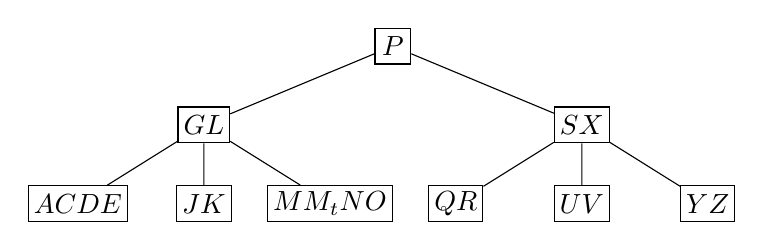
\begin{tikzpicture}[
	level 1/.style={level distance=10mm,sibling distance=48mm},
	level 2/.style={level distance=10mm,sibling distance=16mm},
	level 3/.style={level distance=10mm,sibling distance=16mm},
	inner sep=2pt,every node/.style={draw,rectangle,minimum size=3ex}]
  \node {$P$}
	child {node {$GL$}
		child {node {$ACDE$}}
		child {node {$JK$}}
		child {node {$MM_tNO$}}
	}
  	child {node {$SX$}
	  	child {node {$QR$}}
		child {node {$UV$}}
		child {node {$YZ$}}
	}
;
\end{tikzpicture}

\


%%%%%
\subsubsection{S18 \#L1}
	Given the initial B-tree with the minimum node degree of $t=3$ below, show the results 
	
	\begin{enumerate}[label=\alph*.]
		\item After deleting the key of $M_2$, 
		\item Followed by inserting the key of $L$, 
		\item Then by deleting the key of $J_2$, 
		\item Then by inserting the key of $O_1$ with $O < O_1 < O_2$, and 
		\item Then by deleting $K$.  
	\end{enumerate}
	
	(Show the result after every deletion and after every insertion.)
	
\
	
\hfil	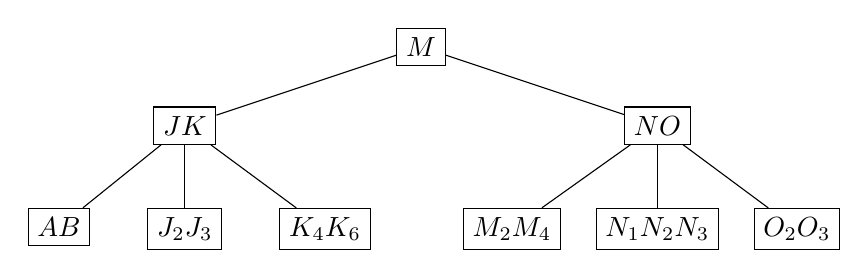
\begin{tikzpicture}[node distance=8 mm and 8 mm]
		\node [rectangle, draw] (a) at (0,0) {$M$};
		\node [rectangle, draw] (b) at (-3,-1) {$J K$};
		\node [rectangle, draw] (c) at (3,-1) {$N O$};
		\node [rectangle, draw, below left=of b] (d) {$A B$};
		\node [rectangle, draw, below=of b] (e) {$J_2 J_3$};
		\node [rectangle, draw, below right=of b] (f) {$K_4 K_6$};
		\node [rectangle, draw, below left=of c] (g) {$M_2 M_4$};
		\node [rectangle, draw, below=of c] (h) {$N_1 N_2 N_3$};
		\node [rectangle, draw, below right=of c] (i) {$O_2 O_3$};
		\foreach \from/\to in {a/b, a/c, b/d, b/e, b/f, c/g, c/h, c/i}
			\draw (\from) -- (\to);
	\end{tikzpicture}
	
	
\subsubsection{Solution}

{\bf Original Tree}

\

\hfil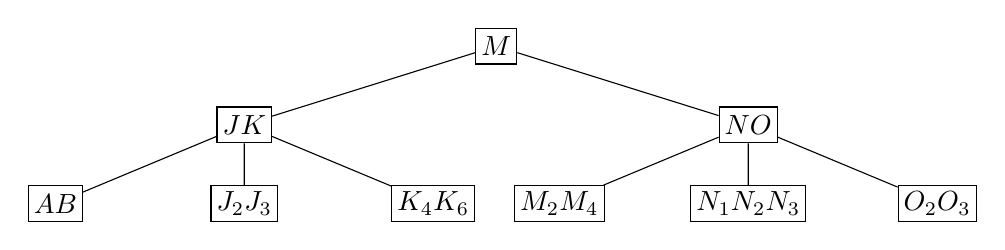
\begin{tikzpicture}[
	level 1/.style={level distance=10mm,sibling distance=64mm},
	level 2/.style={level distance=10mm,sibling distance=24mm},
	level 3/.style={level distance=10mm,sibling distance=16mm},
	inner sep=2pt,every node/.style={draw,rectangle,minimum size=3ex}]
  \node {$M$}
	child {node {$JK$}
		child {node {$AB$}}
		child {node {$J_2 J_3$}}
		child {node {$K_4 K_6$}}
	}
	child {node {$NO$}
		child {node {$M_2 M_4$}}
		child {node {$N_1 N_2 N_3$}}
		child {node {$O_2 O_3$}}
	}
;
\end{tikzpicture}

\

{\bf a. Delete $M_2$.} 

Start on node $M$.  

Instructions on page 502.  

``3.  If the key $k$ [$M_2$] is not present in internal node $x$ [$M$] determine the node $x.c_i$ [$x.c_2 = NO$] of the appropriate subtree that must contain $k$ [$M_2$], if $k$ is in the tree at all.  If $x.c_i$ has only $t-1$ [2] keys, [TRUE], execute step 3a or 3b as necessary to guarantee that we descend to a node containing at least $t$ [3] keys.  Then finish by recursing on the appropriate child of $x$.  

3b.  If $x.c_i$ and both of $x.c_i$'s immediate siblings have $t-1$ [2] keys, merge $x.c_i$ with one sibling, which involves moving a key from $x$ down into the new merged node to become the median key for that node.''  

Consolidate $JK$, $M$, and $NO$.

\

\hfil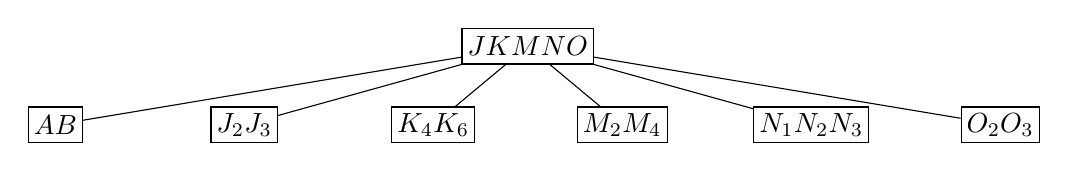
\begin{tikzpicture}[
	level 1/.style={level distance=10mm,sibling distance=24mm},
	level 2/.style={level distance=10mm,sibling distance=24mm},
	level 3/.style={level distance=10mm,sibling distance=16mm},
	inner sep=2pt,every node/.style={draw,rectangle,minimum size=3ex}]
  \node {$JKMNO$}
		child {node {$AB$}}
		child {node {$J_2 J_3$}}
		child {node {$K_4 K_6$}}
		child {node {$M_2M_4$}}
		child {node {$N_1 N_2 N_3$}}
		child {node {$O_2 O_3$}}
;
\end{tikzpicture}

\

``3.  If the key $k$ [$M_2$] is not present in internal node $x$ [$JKMNO$] determine the node $x.c_i$ [$x.c_4 = M_2M_4$] of the appropriate subtree that must contain $k$ [$M_2$], if $k$ is in the tree at all.  If $x.c_i$ has only $t-1$ [2] keys, [TRUE], execute step 3a or 3b as necessary to guarantee that we descend to a node containing at least $t$ [3] keys.  Then finish by recursing on the appropriate child of $x$.  

3a.  If $x.c_i$ [$x.c_4 = M_2M_4$] has only $t-1$ keys but has an immediate sibling with at least $t$ [3] keys, [TRUE], give $x.c_i$ an extra key by moving a key from $x$ [$JKMNO$] down into $x.c_i$, moving a key from $x.c_i$'s immediate left or right sibling up into $x$, and moving the appropriate child pointer [$N$] from the sibling into $x.c_i$.''

Move $N_1$ into $JKMNO$, then move $N$ down into $M_2M_4$.  

\

\hfil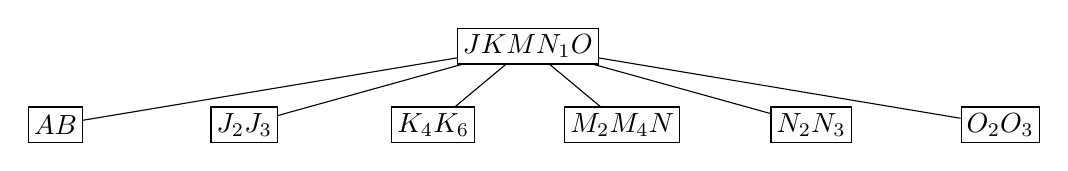
\begin{tikzpicture}[
	level 1/.style={level distance=10mm,sibling distance=24mm},
	level 2/.style={level distance=10mm,sibling distance=24mm},
	level 3/.style={level distance=10mm,sibling distance=16mm},
	inner sep=2pt,every node/.style={draw,rectangle,minimum size=3ex}]
  \node {$JKMN_1O$}
		child {node {$AB$}}
		child {node {$J_2 J_3$}}
		child {node {$K_4 K_6$}}
		child {node {$M_2M_4 N$}}
		child {node {$N_2 N_3$}}
		child {node {$O_2 O_3$}}
;
\end{tikzpicture}

\

Recurse to node $M_2M_4N$.  

``1.  If the key $k$ [$M_2$] is in node $x$ and $x$ is a leaf, [TRUE], delete the node $k$ from $x$.  

\

\hfil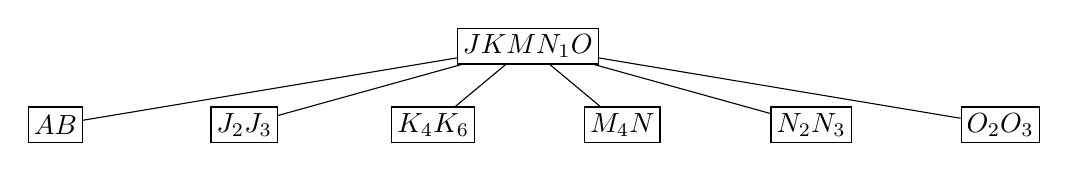
\begin{tikzpicture}[
	level 1/.style={level distance=10mm,sibling distance=24mm},
	level 2/.style={level distance=10mm,sibling distance=24mm},
	level 3/.style={level distance=10mm,sibling distance=16mm},
	inner sep=2pt,every node/.style={draw,rectangle,minimum size=3ex}]
  \node {$JKMN_1O$}
		child {node {$AB$}}
		child {node {$J_2 J_3$}}
		child {node {$K_4 K_6$}}
		child {node {$M_4 N$}}
		child {node {$N_2 N_3$}}
		child {node {$O_2 O_3$}}
;
\end{tikzpicture}

\

{\bf b.  Insert $L$.}  Start by splitting $JKMN_1O$, because it has maximum size and we wouldn't be able to insert something into it if necessary.  

\

\hfil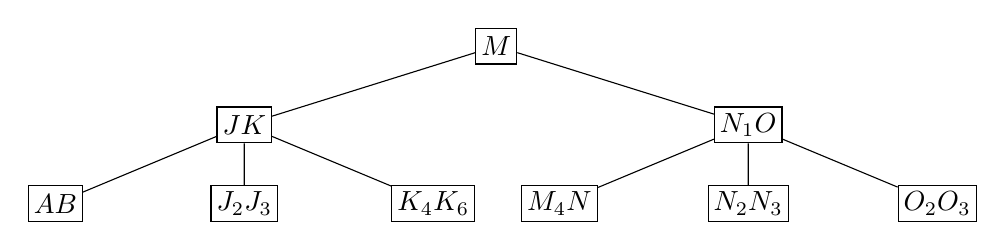
\begin{tikzpicture}[
	level 1/.style={level distance=10mm,sibling distance=64mm},
	level 2/.style={level distance=10mm,sibling distance=24mm},
	level 3/.style={level distance=10mm,sibling distance=16mm},
	inner sep=2pt,every node/.style={draw,rectangle,minimum size=3ex}]
  \node {$M$}
  	child{node{$JK$}
		child {node {$AB$}}
		child {node {$J_2 J_3$}}
		child {node {$K_4 K_6$}}
	}
	child{node{$N_1O$}
		child {node {$M_4 N$}}
		child {node {$N_2 N_3$}}
		child {node {$O_2 O_3$}}
	}
;
\end{tikzpicture}

\

Then it's a leaf insert.  

\

\hfil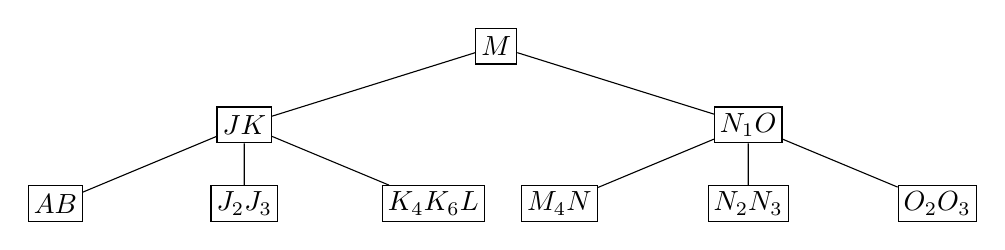
\begin{tikzpicture}[
	level 1/.style={level distance=10mm,sibling distance=64mm},
	level 2/.style={level distance=10mm,sibling distance=24mm},
	level 3/.style={level distance=10mm,sibling distance=16mm},
	inner sep=2pt,every node/.style={draw,rectangle,minimum size=3ex}]
  \node {$M$}
  	child{node{$JK$}
		child {node {$AB$}}
		child {node {$J_2 J_3$}}
		child {node {$K_4 K_6L$}}
	}
	child{node{$N_1O$}
		child {node {$M_4 N$}}
		child {node {$N_2 N_3$}}
		child {node {$O_2 O_3$}}
	}
;
\end{tikzpicture}

\

{\bf c.  Delete $J_2$.}  Re-merge $JK$, $M$, and $N_1O$.  Then rotate $K$ and $K_4$ around to have the minimum number of keys in each node.  

\

\hfil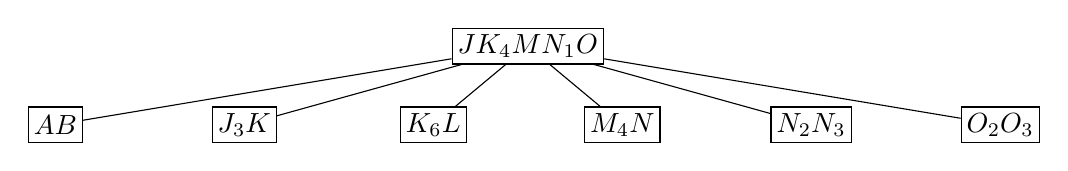
\begin{tikzpicture}[
	level 1/.style={level distance=10mm,sibling distance=24mm},
	level 2/.style={level distance=10mm,sibling distance=24mm},
	level 3/.style={level distance=10mm,sibling distance=16mm},
	inner sep=2pt,every node/.style={draw,rectangle,minimum size=3ex}]
  \node {$JK_4MN_1O$}
		child {node {$AB$}}
		child {node {$J_3 K$}}
		child {node {$K_6 L$}}
		child {node {$M_4 N$}}
		child {node {$N_2 N_3$}}
		child {node {$O_2 O_3$}}
;
\end{tikzpicture}


\

{\bf c.  Insert $O_1$ with $O < O_1 < O_2$.}  Re-split $JK_4MN_1O$, then simple leaf insertion.  

\

\hfil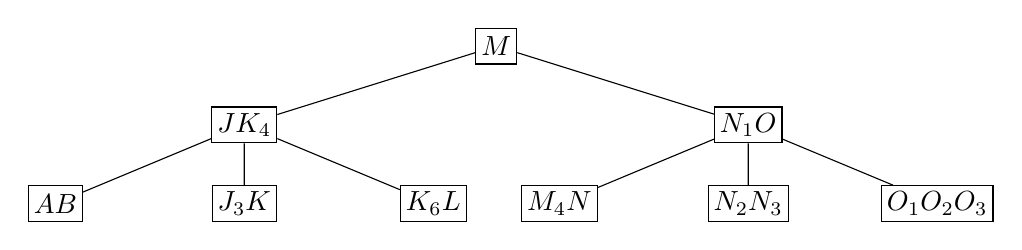
\begin{tikzpicture}[
	level 1/.style={level distance=10mm,sibling distance=64mm},
	level 2/.style={level distance=10mm,sibling distance=24mm},
	level 3/.style={level distance=10mm,sibling distance=16mm},
	inner sep=2pt,every node/.style={draw,rectangle,minimum size=3ex}]
  \node {$M$}
  	child { node{$JK_4$}
		child {node {$AB$}}
		child {node {$J_3 K$}}
		child {node {$K_6 L$}}
	}
	child { node {$N_1O$}
		child {node {$M_4 N$}}
		child {node {$N_2 N_3$}}
		child {node {$O_1 O_2 O_3$}}
	}
;
\end{tikzpicture}


\

{\bf d.  Delete $K$.}  Start with re-merging $JK_4$, $M$, and $N_1O$.    Lots of rotation.  

\

\hfil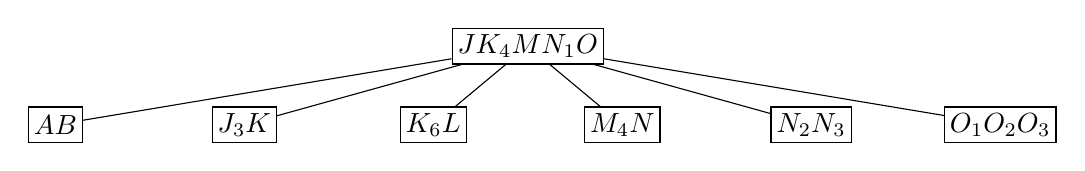
\begin{tikzpicture}[
	level 1/.style={level distance=10mm,sibling distance=24mm},
	level 2/.style={level distance=10mm,sibling distance=24mm},
	level 3/.style={level distance=10mm,sibling distance=16mm},
	inner sep=2pt,every node/.style={draw,rectangle,minimum size=3ex}]
  \node {$JK_4MN_1O$}
		child {node {$AB$}}
		child {node {$J_3 K$}}
		child {node {$K_6 L$}}
		child {node {$M_4 N$}}
		child {node {$N_2 N_3$}}
		child {node {$O_1 O_2 O_3$}}
;
\end{tikzpicture}


\

Rotate  $O$ and $O_1$ left.  

\

\hfil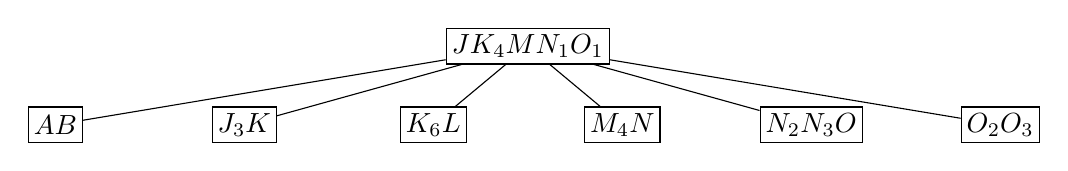
\begin{tikzpicture}[
	level 1/.style={level distance=10mm,sibling distance=24mm},
	level 2/.style={level distance=10mm,sibling distance=24mm},
	level 3/.style={level distance=10mm,sibling distance=16mm},
	inner sep=2pt,every node/.style={draw,rectangle,minimum size=3ex}]
  \node {$JK_4MN_1O_1$}
		child {node {$AB$}}
		child {node {$J_3 K$}}
		child {node {$K_6 L$}}
		child {node {$M_4 N$}}
		child {node {$N_2 N_3O$}}
		child {node {$O_2 O_3$}}
;
\end{tikzpicture}


\

Rotate $N1$ and $N_2$ left.  

\

\hfil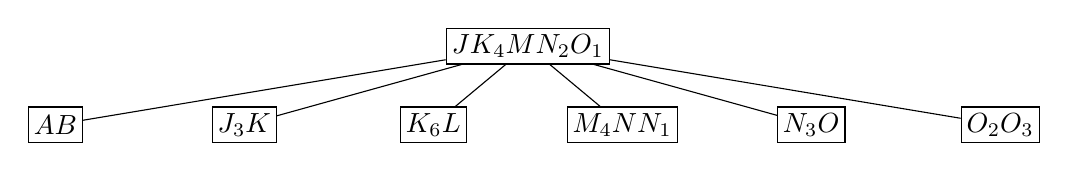
\begin{tikzpicture}[
	level 1/.style={level distance=10mm,sibling distance=24mm},
	level 2/.style={level distance=10mm,sibling distance=24mm},
	level 3/.style={level distance=10mm,sibling distance=16mm},
	inner sep=2pt,every node/.style={draw,rectangle,minimum size=3ex}]
  \node {$JK_4MN_2O_1$}
		child {node {$AB$}}
		child {node {$J_3 K$}}
		child {node {$K_6 L$}}
		child {node {$M_4 N N_1$}}
		child {node {$ N_3O$}}
		child {node {$O_2 O_3$}}
;
\end{tikzpicture}


\

Rotate $M$ and $M_4$ left.  

\

\hfil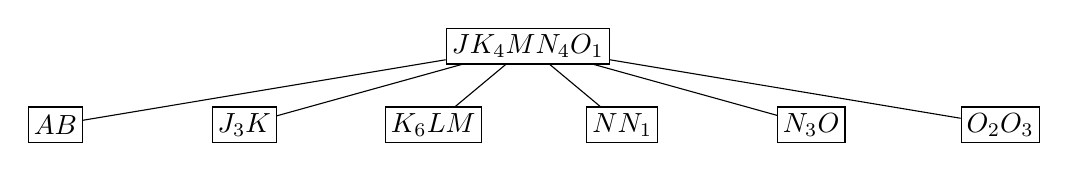
\begin{tikzpicture}[
	level 1/.style={level distance=10mm,sibling distance=24mm},
	level 2/.style={level distance=10mm,sibling distance=24mm},
	level 3/.style={level distance=10mm,sibling distance=16mm},
	inner sep=2pt,every node/.style={draw,rectangle,minimum size=3ex}]
  \node {$JK_4MN_4O_1$}
		child {node {$AB$}}
		child {node {$J_3 K$}}
		child {node {$K_6 L M$}}
		child {node {$N N_1$}}
		child {node {$ N_3O$}}
		child {node {$O_2 O_3$}}
;
\end{tikzpicture}


\

Rotate $K_4$ and $K_6$ left.  

\

\hfil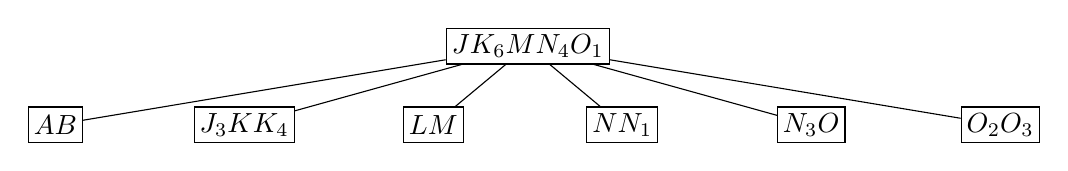
\begin{tikzpicture}[
	level 1/.style={level distance=10mm,sibling distance=24mm},
	level 2/.style={level distance=10mm,sibling distance=24mm},
	level 3/.style={level distance=10mm,sibling distance=16mm},
	inner sep=2pt,every node/.style={draw,rectangle,minimum size=3ex}]
  \node {$JK_6MN_4O_1$}
		child {node {$AB$}}
		child {node {$J_3 K K_4$}}
		child {node {$ L M$}}
		child {node {$N N_1$}}
		child {node {$ N_3O$}}
		child {node {$O_2 O_3$}}
;
\end{tikzpicture}


\

Delete $K$ from the node.

\

\hfil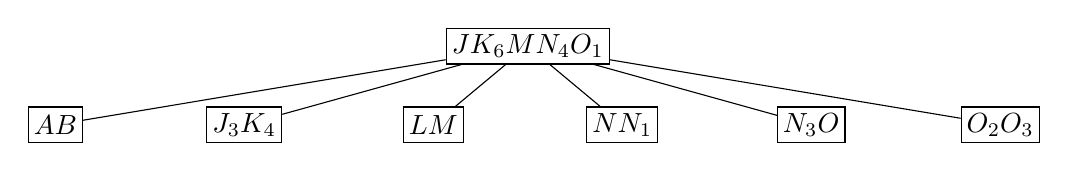
\begin{tikzpicture}[
	level 1/.style={level distance=10mm,sibling distance=24mm},
	level 2/.style={level distance=10mm,sibling distance=24mm},
	level 3/.style={level distance=10mm,sibling distance=16mm},
	inner sep=2pt,every node/.style={draw,rectangle,minimum size=3ex}]
  \node {$JK_6MN_4O_1$}
		child {node {$AB$}}
		child {node {$J_3 K_4$}}
		child {node {$ L M$}}
		child {node {$N N_1$}}
		child {node {$ N_3O$}}
		child {node {$O_2 O_3$}}
;
\end{tikzpicture}


\







%%%%%
\subsubsection{F18 \#L2}
	Given the initial B-tree with the minimum node degree of $t=3$ below, show the results 
	
	\begin{enumerate}[label=\alph*.]
		\item After deleting the key of $K$, 
		\item Followed by inserting the key of $L$, 
		\item Then by deleting the key of $J_2$, 
		\item Then by inserting the key of $N_4$ with $N_3 < N_4 < O$, and 
		\item Then by deleting $K_4$.  
	\end{enumerate}
	
	(Show the result after every deletion and after every insertion.)
	
\
	
\hfil	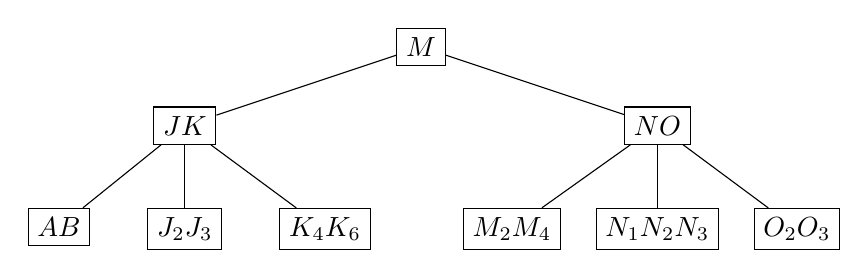
\begin{tikzpicture}[node distance=8 mm and 8 mm]
		\node [rectangle, draw] (a) at (0,0) {$M$};
		\node [rectangle, draw] (b) at (-3,-1) {$J K$};
		\node [rectangle, draw] (c) at (3,-1) {$N O$};
		\node [rectangle, draw, below left=of b] (d) {$A B$};
		\node [rectangle, draw, below=of b] (e) {$J_2 J_3$};
		\node [rectangle, draw, below right=of b] (f) {$K_4 K_6$};
		\node [rectangle, draw, below left=of c] (g) {$M_2 M_4$};
		\node [rectangle, draw, below=of c] (h) {$N_1 N_2 N_3$};
		\node [rectangle, draw, below right=of c] (i) {$O_2 O_3$};
		\foreach \from/\to in {a/b, a/c, b/d, b/e, b/f, c/g, c/h, c/i}
			\draw (\from) -- (\to);
	\end{tikzpicture}

\

Note:  Same tree as in S18 \#L1, but different keys to insert and delete.  

\subsubsection{Solution}

{\bf Original Tree}

\

\hfil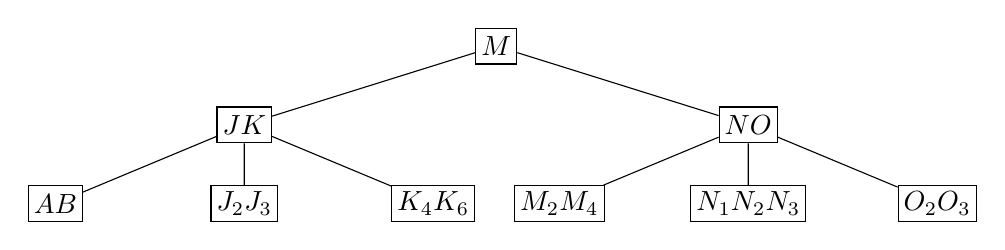
\begin{tikzpicture}[
	level 1/.style={level distance=10mm,sibling distance=64mm},
	level 2/.style={level distance=10mm,sibling distance=24mm},
	level 3/.style={level distance=10mm,sibling distance=16mm},
	inner sep=2pt,every node/.style={draw,rectangle,minimum size=3ex}]
  \node {$M$}
	child {node {$JK$}
		child {node {$AB$}}
		child {node {$J_2 J_3$}}
		child {node {$K_4 K_6$}}
	}
	child {node {$NO$}
		child {node {$M_2 M_4$}}
		child {node {$N_1 N_2 N_3$}}
		child {node {$O_2 O_3$}}
	}
;
\end{tikzpicture}

\

{\bf a.  Delete $K$.}  First, merge $JK$, $M$, and $NO$.  

\

\hfil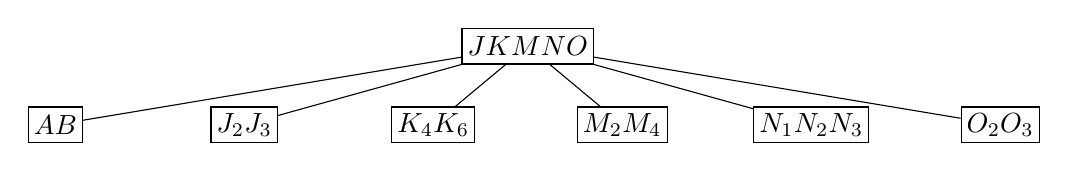
\begin{tikzpicture}[
	level 1/.style={level distance=10mm,sibling distance=24mm},
	level 2/.style={level distance=10mm,sibling distance=24mm},
	level 3/.style={level distance=10mm,sibling distance=16mm},
	inner sep=2pt,every node/.style={draw,rectangle,minimum size=3ex}]
  \node {$JKMNO$}
		child {node {$AB$}}
		child {node {$J_2 J_3$}}
		child {node {$K_4 K_6$}}
		child {node {$M_2M_4$}}
		child {node {$N_1 N_2 N_3$}}
		child {node {$O_2 O_3$}}
;
\end{tikzpicture}

\

Then delete $K$ and merge $J_2 J_3$ and $K_4 K_6$.

\

\hfil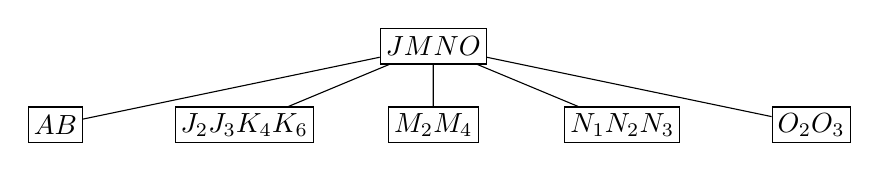
\begin{tikzpicture}[
	level 1/.style={level distance=10mm,sibling distance=24mm},
	level 2/.style={level distance=10mm,sibling distance=24mm},
	level 3/.style={level distance=10mm,sibling distance=16mm},
	inner sep=2pt,every node/.style={draw,rectangle,minimum size=3ex}]
  \node {$JMNO$}
		child {node {$AB$}}
		child {node {$J_2 J_3 K_4 K_6$}}
		child {node {$M_2M_4$}}
		child {node {$N_1 N_2 N_3$}}
		child {node {$O_2 O_3$}}
;
\end{tikzpicture}

\

{\bf b.  Insert $L$.}  Just a simple leaf insert.  

\

\hfil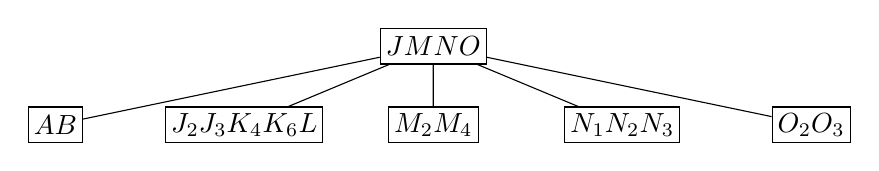
\begin{tikzpicture}[
	level 1/.style={level distance=10mm,sibling distance=24mm},
	level 2/.style={level distance=10mm,sibling distance=24mm},
	level 3/.style={level distance=10mm,sibling distance=16mm},
	inner sep=2pt,every node/.style={draw,rectangle,minimum size=3ex}]
  \node {$JMNO$}
		child {node {$AB$}}
		child {node {$J_2 J_3 K_4 K_6 L$}}
		child {node {$M_2M_4$}}
		child {node {$N_1 N_2 N_3$}}
		child {node {$O_2 O_3$}}
;
\end{tikzpicture}


\

{\bf c.  Delete $J_2$.}  Just a simple leaf deletion.

\

\hfil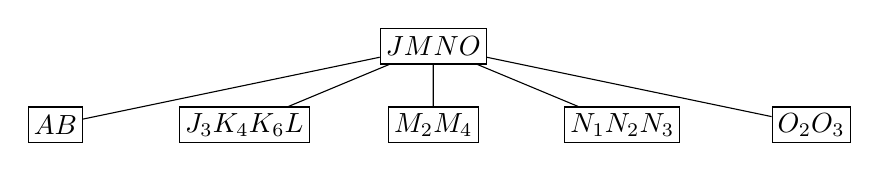
\begin{tikzpicture}[
	level 1/.style={level distance=10mm,sibling distance=24mm},
	level 2/.style={level distance=10mm,sibling distance=24mm},
	level 3/.style={level distance=10mm,sibling distance=16mm},
	inner sep=2pt,every node/.style={draw,rectangle,minimum size=3ex}]
  \node {$JMNO$}
		child {node {$AB$}}
		child {node {$J_3 K_4 K_6 L$}}
		child {node {$M_2M_4$}}
		child {node {$N_1 N_2 N_3$}}
		child {node {$O_2 O_3$}}
;
\end{tikzpicture}

\


{\bf d.  Insert $N_4$ with $N_3 < N_4 < O$.}  Just a simple leaf insertion.

\

\hfil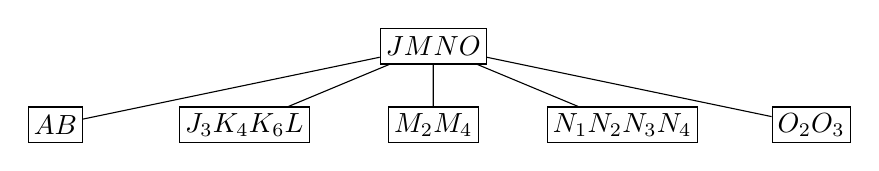
\begin{tikzpicture}[
	level 1/.style={level distance=10mm,sibling distance=24mm},
	level 2/.style={level distance=10mm,sibling distance=24mm},
	level 3/.style={level distance=10mm,sibling distance=16mm},
	inner sep=2pt,every node/.style={draw,rectangle,minimum size=3ex}]
  \node {$JMNO$}
		child {node {$AB$}}
		child {node {$J_3 K_4 K_6 L$}}
		child {node {$M_2M_4$}}
		child {node {$N_1 N_2 N_3 N_4$}}
		child {node {$O_2 O_3$}}
;
\end{tikzpicture}

\


{\bf e.  Delete $K_4$.}  Just a simple leaf deletion.

\

\hfil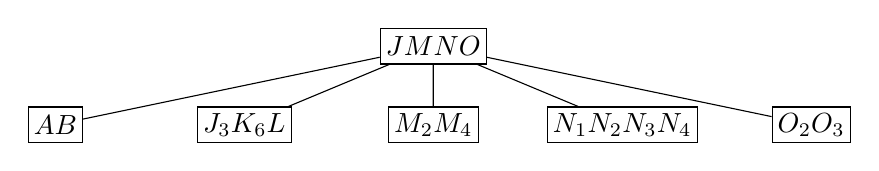
\begin{tikzpicture}[
	level 1/.style={level distance=10mm,sibling distance=24mm},
	level 2/.style={level distance=10mm,sibling distance=24mm},
	level 3/.style={level distance=10mm,sibling distance=16mm},
	inner sep=2pt,every node/.style={draw,rectangle,minimum size=3ex}]
  \node {$JMNO$}
		child {node {$AB$}}
		child {node {$J_3 K_6 L$}}
		child {node {$M_2M_4$}}
		child {node {$N_1 N_2 N_3 N_4$}}
		child {node {$O_2 O_3$}}
;
\end{tikzpicture}

\

%%%%%	
\subsubsection{F16 \#L3}
	Given an initial B-tree with the minimum node degree of $t=2$ below, show the results 
	\begin{enumerate}
		\item after inserting the key of $H$, and 
		\item then followed by deleting two keys in order:  $X$ then $P$.  (show the result after insertion and the result after each deletion.)
	\end{enumerate}
	
\
	
\hfil	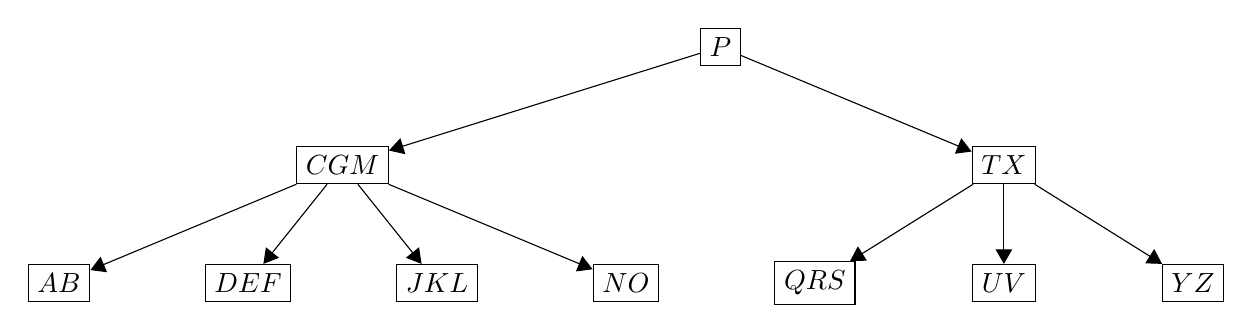
\begin{tikzpicture}[x=12mm, y=15mm]
		\node [rectangle, draw] (0) at (0,0) {$P$};
		\node [rectangle, draw] (1) at (-4,-1) {$C G M$};
		\node [rectangle, draw] (2) at (3,-1) {$T X$};
		\node [rectangle, draw] (3) at (-7,-2) {$A B$};
		\node [rectangle, draw] (4) at (-5,-2) {$D E F$};
		\node [rectangle, draw] (5) at (-3,-2) {$J K L$};
		\node [rectangle, draw] (6) at (-1,-2) {$N O$};
		\node [rectangle, draw] (7) at (1,-2) {$Q R S$};
		\node [rectangle, draw] (8) at (3,-2) {$U V$};
		\node [rectangle, draw] (9) at (5,-2) {$Y Z$};
		\draw [-triangle 60] (0) -- (1); 
		\draw [-triangle 60] (0) -- (2); 
		\draw [-triangle 60] (1) -- (3); 
		\draw [-triangle 60] (1) -- (4); 
		\draw [-triangle 60] (1) -- (5); 
		\draw [-triangle 60] (1) -- (6); 
		\draw [-triangle 60] (2) -- (7); 
		\draw [-triangle 60] (2) -- (8); 
		\draw [-triangle 60] (2) -- (9); 
	\end{tikzpicture}
	
\subsubsection{Solution}

{\bf Original Tree}

\	
	
\hfil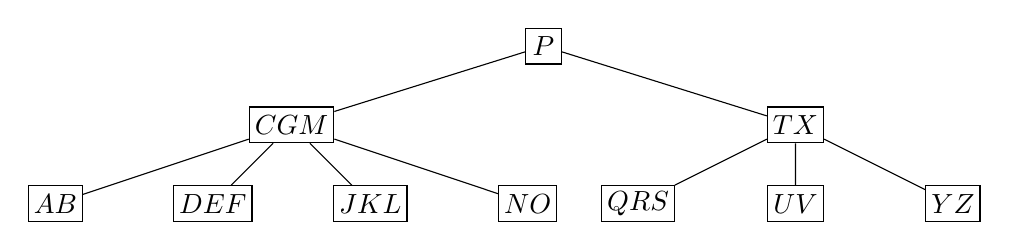
\begin{tikzpicture}[
	level 1/.style={level distance=10mm,sibling distance=64mm},
	level 2/.style={level distance=10mm,sibling distance=20mm},
	level 3/.style={level distance=10mm,sibling distance=16mm},
	inner sep=2pt,every node/.style={draw,rectangle,minimum size=3ex}]
  \node {$P$}
		child {node {$CGM$}
			child {node {$AB$}}
			child {node {$DEF$}}
			child {node {$JKL$}}
			child {node {$NO$}}
		}
		child {node {$TX$}
			child {node {$QRS$}}
			child {node {$UV$}}
			child {node {$YZ$}}
		}
;
\end{tikzpicture}

\

{\bf Insert $H$.}  As we go down the tree toward where $H$ should go, we encounter a full node, $CGM$, so we have to split it.  

\	
	
\hfil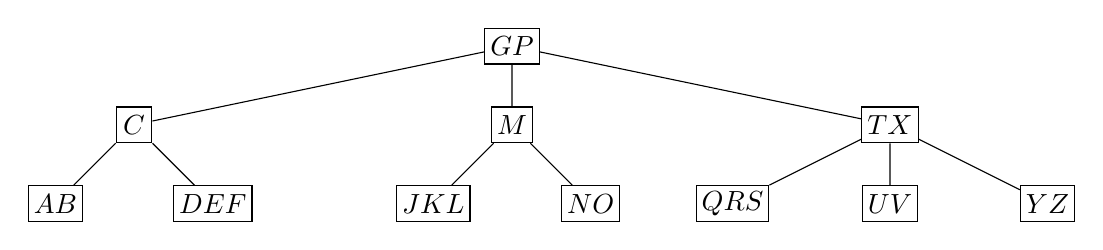
\begin{tikzpicture}[
	level 1/.style={level distance=10mm,sibling distance=48mm},
	level 2/.style={level distance=10mm,sibling distance=20mm},
	level 3/.style={level distance=10mm,sibling distance=16mm},
	inner sep=2pt,every node/.style={draw,rectangle,minimum size=3ex}]
  \node {$GP$}
		child {node {$C$}
			child {node {$AB$}}
			child {node {$DEF$}}
		}
		child {node {$M$}
			child {node {$JKL$}}
			child {node {$NO$}}
		}
		child {node {$TX$}
			child {node {$QRS$}}
			child {node {$UV$}}
			child {node {$YZ$}}
		}
;
\end{tikzpicture}

\

Then going down we want to insert $H$ in $JKL$, but it is full, so we have to split it.  

\	
	
\hfil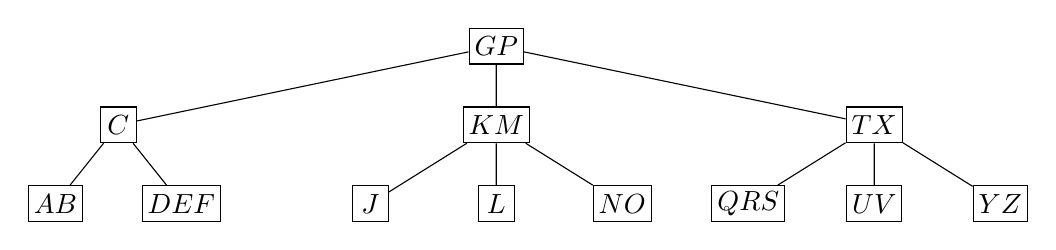
\begin{tikzpicture}[
	level 1/.style={level distance=10mm,sibling distance=48mm},
	level 2/.style={level distance=10mm,sibling distance=16mm},
	level 3/.style={level distance=10mm,sibling distance=16mm},
	inner sep=2pt,every node/.style={draw,rectangle,minimum size=3ex}]
  \node {$GP$}
		child {node {$C$}
			child {node {$AB$}}
			child {node {$DEF$}}
		}
		child {node {$KM$}
			child {node {$J$}}
			child {node {$L$}}
			child {node {$NO$}}
		}
		child {node {$TX$}
			child {node {$QRS$}}
			child {node {$UV$}}
			child {node {$YZ$}}
		}
;
\end{tikzpicture}

\

Now we can insert $H$.  


\	
	
\hfil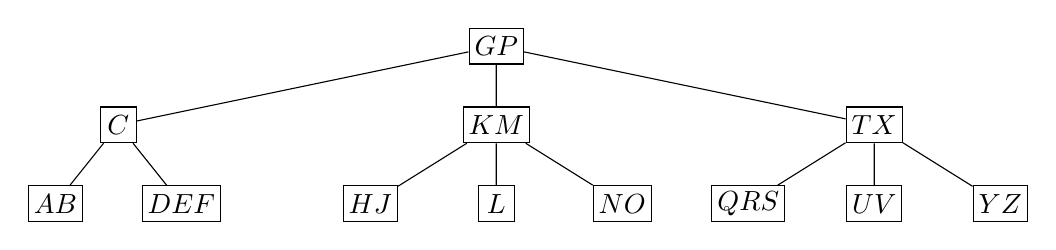
\begin{tikzpicture}[
	level 1/.style={level distance=10mm,sibling distance=48mm},
	level 2/.style={level distance=10mm,sibling distance=16mm},
	level 3/.style={level distance=10mm,sibling distance=16mm},
	inner sep=2pt,every node/.style={draw,rectangle,minimum size=3ex}]
  \node {$GP$}
		child {node {$C$}
			child {node {$AB$}}
			child {node {$DEF$}}
		}
		child {node {$KM$}
			child {node {$HJ$}}
			child {node {$L$}}
			child {node {$NO$}}
		}
		child {node {$TX$}
			child {node {$QRS$}}
			child {node {$UV$}}
			child {node {$YZ$}}
		}
;
\end{tikzpicture}

	
\

{\bf Delete $X$.}  Move $V$ up.  
	


\	
	
\hfil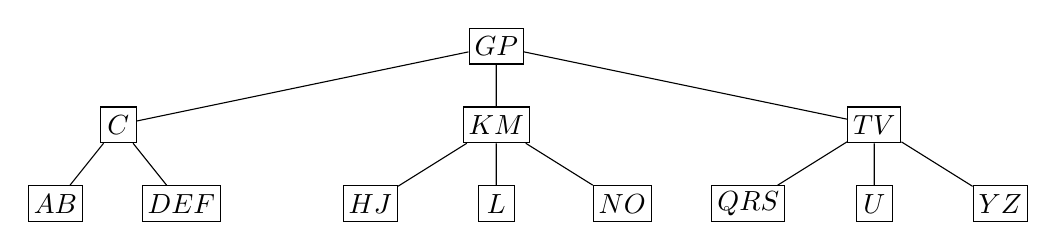
\begin{tikzpicture}[
	level 1/.style={level distance=10mm,sibling distance=48mm},
	level 2/.style={level distance=10mm,sibling distance=16mm},
	level 3/.style={level distance=10mm,sibling distance=16mm},
	inner sep=2pt,every node/.style={draw,rectangle,minimum size=3ex}]
  \node {$GP$}
		child {node {$C$}
			child {node {$AB$}}
			child {node {$DEF$}}
		}
		child {node {$KM$}
			child {node {$HJ$}}
			child {node {$L$}}
			child {node {$NO$}}
		}
		child {node {$TV$}
			child {node {$QRS$}}
			child {node {$U$}}
			child {node {$YZ$}}
		}
;
\end{tikzpicture}

	
\

	
\

{\bf Delete $P$.}  Move $O$ up.  
	


\	
	
\hfil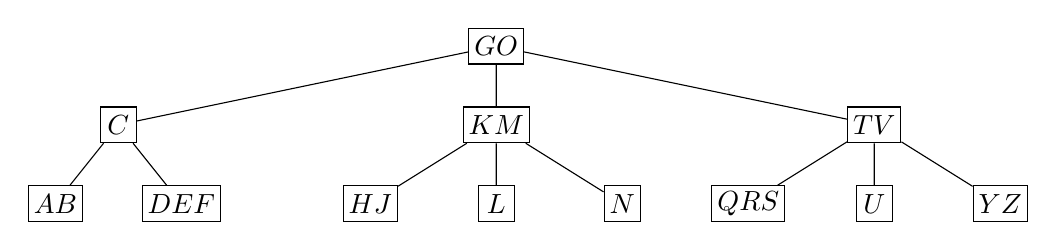
\begin{tikzpicture}[
	level 1/.style={level distance=10mm,sibling distance=48mm},
	level 2/.style={level distance=10mm,sibling distance=16mm},
	level 3/.style={level distance=10mm,sibling distance=16mm},
	inner sep=2pt,every node/.style={draw,rectangle,minimum size=3ex}]
  \node {$GO$}
		child {node {$C$}
			child {node {$AB$}}
			child {node {$DEF$}}
		}
		child {node {$KM$}
			child {node {$HJ$}}
			child {node {$L$}}
			child {node {$N$}}
		}
		child {node {$TV$}
			child {node {$QRS$}}
			child {node {$U$}}
			child {node {$YZ$}}
		}
;
\end{tikzpicture}

	
\

%%%%%
\subsubsection{F15 \#S8}
	For any $n$-key B-tree of height $h$ and with minimum node degree of $t \ge 2$, prove that $h$ is no larger than $\log_t \frac{n+1}{2}$.  (Hint:  Consider the number of keys stored in each tree level.)
	
	

\subsubsection{Solution}	

For illustration, take $t=3$.  In each node is the minimum number of keys in the node.

We're interested in the {\it minimum} number of keys per node, so that we get the maximum possible height for $n$ keys, giving us an upper bound for the height of the tree.  



\


	
\hfil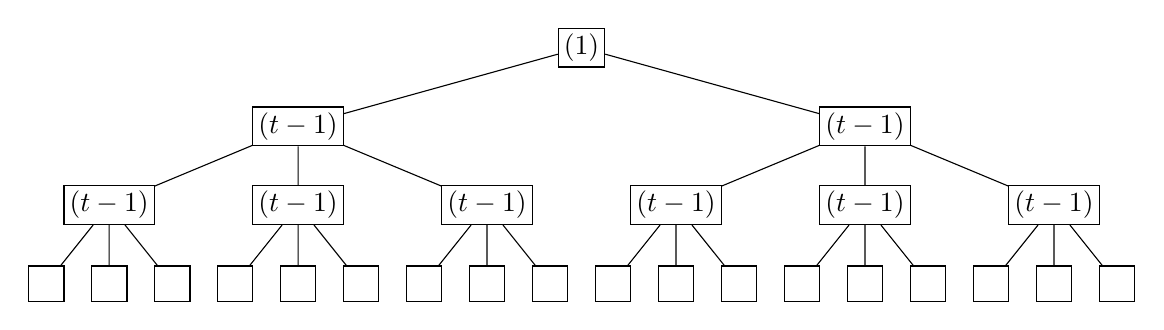
\begin{tikzpicture}[
	level 1/.style={level distance=10mm,sibling distance=72mm},
	level 2/.style={level distance=10mm,sibling distance=24mm},
	level 3/.style={level distance=10mm,sibling distance=8mm},
	inner sep=2pt,every node/.style={draw,rectangle,minimum size=3ex}]
  \node {$(1)$}
		child {node {$(t-1)$}
			child {node {$(t-1)$}
				child {node {}}
				child {node {}}
				child {node {}}
			}
			child {node {$(t-1)$}
				child {node {}}
				child {node {}}
				child {node {}}
			}
			child {node {$(t-1)$}
				child {node {$$}}
				child {node {$$}}
				child {node {$$}}
			}
		}
		child {node {$(t-1)$}
			child {node {$(t-1)$}
				child {node {$$}}
				child {node {$$}}
				child {node {$$}}
			}
			child {node {$(t-1)$}
				child {node {$$}}
				child {node {$$}}
				child {node {$$}}
			}
			child {node {$(t-1)$}
				child {node {$$}}
				child {node {$$}}
				child {node {$$}}
			}
		}
	
;
\end{tikzpicture}

\

The root node (depth 0) has at least one key; thus, two children.  At depth 1, each of the two nodes has at least $t-1$ keys; thus, $t$ children.  At any greater depth, each node has at least $t-1$ keys; thus, $t$ children.  

\

\begin{tabular}{ccc}
	& \multicolumn{2}{c}{Minimum Number of} \cr\cline{2-3}
	Depth & Nodes & Keys \cr\hline
	0 & 1  & 1 \cr
	1 & 2 & $2(t-1)$ \cr
	2 & $2t$ & $2t(t-1)$ \cr
	3 & $2t^2$ & $2t^2(t-1)$ \cr
	& $\vdots$ & \cr
	$h$ & $2t^{h-1}$ & $2t^{h-1}(t-1)$ \cr
\end{tabular}
	
\begin{align*}
	1 + 2(t-1) + 2t(t-1) + 2t^2(t-1) + \cdots + 2t^{h-1}(t-1) &= n \cr
	2(t-1)(1 + t + t^2 + \cdots + t^{h-1}) &= n-1 \cr
	(t-1)\left( \frac{t^h - 1}{t-1} \right) &= \frac{n-1}{2} \cr
	t^h - 1 &= \frac{n-1}{2} \cr
	t^h &= \frac{n-1}{2} + 1 \cr
	t^h &= \frac{n+1}{2} \cr
	 h &= \log_t \frac{n+1}{2} \cr
\end{align*}

\subsubsection{Related Question}

For any $n$-key B-tree of height $h$ and with minimum node degree of $t\ge 2$, find the minimum value of $h$, the height of the tree.  

\

\begin{tabular}{*3{>{$}c<{$}}}
	& \multicolumn{2}{c}{Maximum Number of} \cr\cline{2-3}
	\text{Depth} & \text{Nodes} & \text{Keys} \cr\hline
	0 & 1 & 2t-1 \cr
	1 & 2t & 2t(2t-1) \cr
	2 & (2t)^2 & (2t)^2(2t-1) \cr
	& \vdots \cr
	h & (2t)^h & (2t)^h(2t-1) \cr
\end{tabular}
	
\begin{align*} 
	(2t-1) + 2t(2t-1) + (2t)^2(2t-1) + \cdots (2t)^h(2t-1) &= n \cr
	(2t-1)(1 + (2t) + (2t)^2 + (2t)^h) &= n \cr
	(2t-1)\left( \frac{(2t)^{h+1} - 1}{2t-1} \right) &= n \cr
	(2t)^{h+1} - 1 &= n \cr
	(2t)^{h+1} &= n+1 \cr
	h+1 &= \log_{2t} (n+1) \cr
	h &= \log_{2t}(n+1) - 1 \cr
\end{align*}

\

For any $n$-key B-tree of height $h$ and minimum node degree of $t\ge 2$, 

$$\log_{2t}(n+1) - 1 \le h \le \log_t \frac{n+1}{2}$$

For instance, if $t=2$ and $n=63$, then the height is between 2 and 5.  

$$\log_{2t}(n+1) - 1  = \log_4 64 = 3, \qquad \log_t\frac{n+1}{2} = \log_2 32 = 5$$

%%%%%	
\subsubsection{F15 \#L2}
	Given the initial B-tree with the minimum node degree of $t=3$ below, show the results (a) after inserting two keys in order:  $Q$ then $W$, and (b) followed by deleting two keys in order:  $Y$ then $T$.  (Show the aggregate result after insertion and another result after deletion.)
	
	\
	
\hfil	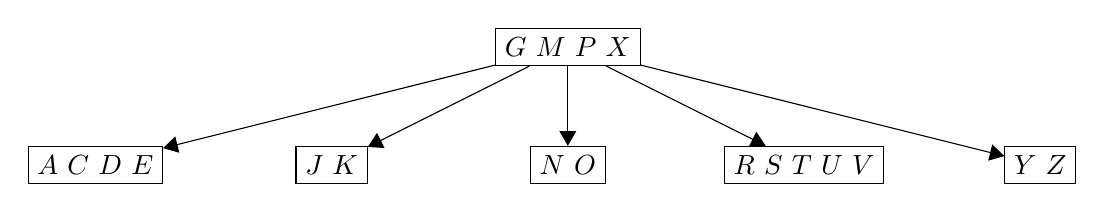
\begin{tikzpicture}[x=15mm, y=15mm]
		\node [rectangle, draw] (GMPX) at (0,0) {$G \ M \ P \ X$};
		\node [rectangle, draw] (ACDE) at (-4,-1) {$A \ C \ D \ E$};
		\node [rectangle, draw] (JK) at (-2,-1) {$J \ K$};
		\node [rectangle, draw] (NO) at (0,-1) {$N \ O$};
		\node [rectangle, draw] (RSTUV) at (2,-1) {$R \ S \ T \ U \ V$};
		\node [rectangle, draw] (YZ) at (4,-1) {$Y \ Z$};
		\foreach \from/\to in {GMPX/ACDE, GMPX/JK, GMPX/NO, GMPX/RSTUV, GMPX/YZ}
			\draw [-triangle 60] (\from) -- (\to);
	\end{tikzpicture}
	
\subsubsection{Solution}
 
\hfil 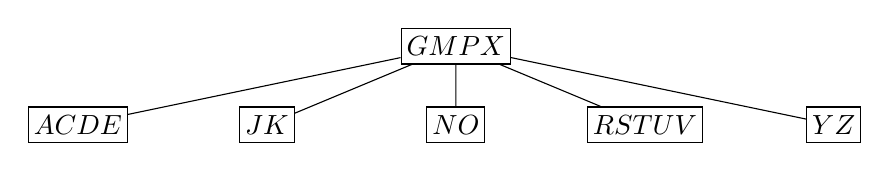
\begin{tikzpicture}[
	level 1/.style={level distance=10mm,sibling distance=24mm},
	level 2/.style={level distance=10mm,sibling distance=24mm},
	level 3/.style={level distance=10mm,sibling distance=8mm},
	inner sep=2pt,every node/.style={draw,rectangle,minimum size=3ex}]
	\node {$GMPX$}
  		child {node {$ACDE$}}
  		child {node {$JK$}}
  		child {node {$NO$}}
  		child {node {$RSTUV$}}
  		child {node {$YZ$}}
	;
\end{tikzpicture}

\	
	
To insert $Q$, we note that $RSTUV$ is full, because $x.n = 5 = 2t-1$, so we must split it by moving $T$ up.  	

\
	
\hfil 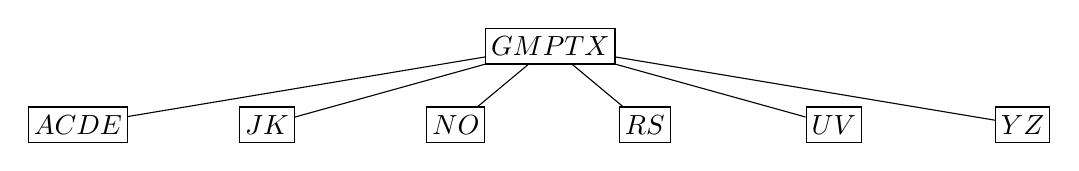
\begin{tikzpicture}[
	level 1/.style={level distance=10mm,sibling distance=24mm},
	level 2/.style={level distance=10mm,sibling distance=24mm},
	level 3/.style={level distance=10mm,sibling distance=8mm},
	inner sep=2pt,every node/.style={draw,rectangle,minimum size=3ex}]
	\node {$GMPTX$}
  		child {node {$ACDE$}}
  		child {node {$JK$}}
  		child {node {$NO$}}
  		child {node {$RS$}}
  		child {node {$UV$}}
  		child {node {$YZ$}}
	;
\end{tikzpicture}	

\
	
Then insert $Q$ into a leaf, simple leaf insertion.  	


\
	
\hfil 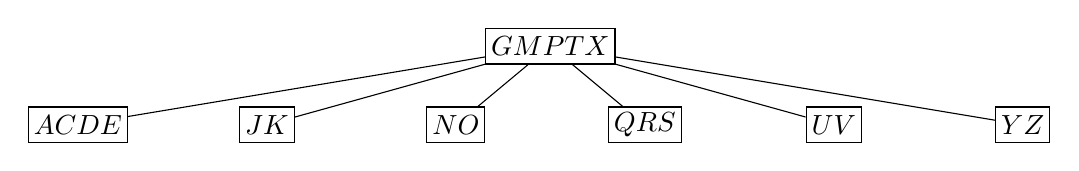
\begin{tikzpicture}[
	level 1/.style={level distance=10mm,sibling distance=24mm},
	level 2/.style={level distance=10mm,sibling distance=24mm},
	level 3/.style={level distance=10mm,sibling distance=8mm},
	inner sep=2pt,every node/.style={draw,rectangle,minimum size=3ex}]
	\node {$GMPTX$}
  		child {node {$ACDE$}}
  		child {node {$JK$}}
  		child {node {$NO$}}
  		child {node {$QRS$}}
  		child {node {$UV$}}
  		child {node {$YZ$}}
	;
\end{tikzpicture}	
	
\

When we go to make another insertion, we hit a full node, $GMPSX$, so we must split it first.  
	

\
	
\hfil 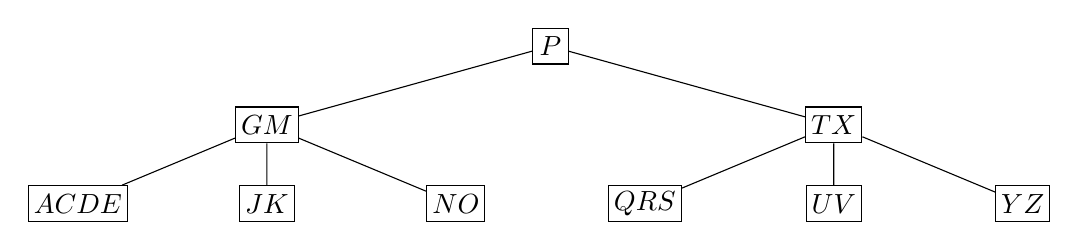
\begin{tikzpicture}[
	level 1/.style={level distance=10mm,sibling distance=72mm},
	level 2/.style={level distance=10mm,sibling distance=24mm},
	level 3/.style={level distance=10mm,sibling distance=8mm},
	inner sep=2pt,every node/.style={draw,rectangle,minimum size=3ex}]
	\node {$P$}
		child {node {$GM$}
	  		child {node {$ACDE$}}
	  		child {node {$JK$}}
	  		child {node {$NO$}}
		}
		child {node {$TX$}
	  		child {node {$QRS$}}
	  		child {node {$UV$}}
	  		child {node {$YZ$}}
		}
	;
\end{tikzpicture}	
	
\

Now $W$ is a simple leaf insertion.  	
	

\
	
\hfil 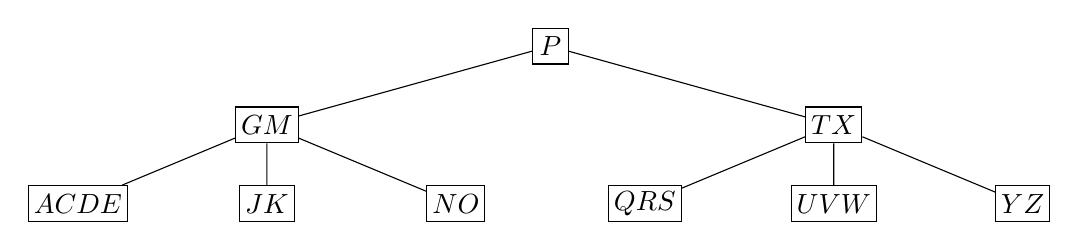
\begin{tikzpicture}[
	level 1/.style={level distance=10mm,sibling distance=72mm},
	level 2/.style={level distance=10mm,sibling distance=24mm},
	level 3/.style={level distance=10mm,sibling distance=8mm},
	inner sep=2pt,every node/.style={draw,rectangle,minimum size=3ex}]
	\node {$P$}
		child {node {$GM$}
	  		child {node {$ACDE$}}
	  		child {node {$JK$}}
	  		child {node {$NO$}}
		}
		child {node {$TX$}
	  		child {node {$QRS$}}
	  		child {node {$UVW$}}
	  		child {node {$YZ$}}
		}
	;
\end{tikzpicture}	
	
\

When we want to delete a key ($Y$), going down the graph we see that we can re-merge $GM$, $P$, and $TX$.  


\
	
\hfil \begin{tikzpicture}[
	level 1/.style={level distance=10mm,sibling distance=24mm},
	level 2/.style={level distance=10mm,sibling distance=24mm},
	level 3/.style={level distance=10mm,sibling distance=8mm},
	inner sep=2pt,every node/.style={draw,rectangle,minimum size=3ex}]
	\node {$GMPTX$}
  		child {node {$ACDE$}}
  		child {node {$JK$}}
  		child {node {$NO$}}
  		child {node {$QRS$}}
  		child {node {$UVW$}}
  		child {node {$YZ$}}
	;
\end{tikzpicture}	
	
\

Now delete $Y$ by rotating $W$ and $X$ around to the right.  	


\
	
\hfil \begin{tikzpicture}[
	level 1/.style={level distance=10mm,sibling distance=24mm},
	level 2/.style={level distance=10mm,sibling distance=24mm},
	level 3/.style={level distance=10mm,sibling distance=8mm},
	inner sep=2pt,every node/.style={draw,rectangle,minimum size=3ex}]
	\node {$GMPTW$}
  		child {node {$ACDE$}}
  		child {node {$JK$}}
  		child {node {$NO$}}
  		child {node {$QRS$}}
  		child {node {$UV$}}
  		child {node {$XZ$}}
	;
\end{tikzpicture}	
	
\

To delete $T$, just merge $QRS$ and $UV$.  

\
	
\hfil \begin{tikzpicture}[
	level 1/.style={level distance=10mm,sibling distance=24mm},
	level 2/.style={level distance=10mm,sibling distance=24mm},
	level 3/.style={level distance=10mm,sibling distance=8mm},
	inner sep=2pt,every node/.style={draw,rectangle,minimum size=3ex}]
	\node {$GMPW$}
  		child {node {$ACDE$}}
  		child {node {$JK$}}
  		child {node {$NO$}}
  		child {node {$QRSUV$}}
  		child {node {$XZ$}}
	;
\end{tikzpicture}	
	
\

	
	
	
	
	
	


\section{Binary Search Trees}

\subsection{Definition, Chapter 12}

\index{Binary Search Tree!Definition \S 12}

The linked data structure in which every node is an object has a $key$ and attributes $left$, $right$, and $p$ that point to the nodes of the left child, right child, and parent.  If the node does not have such an attribute, its value is \verb|NIL|.  The root node is the only node whose parent is \verb|NIL|.

\

Binary Search Tree Property.  Let $x$ be a node in a binary search tree.  If $y$ is a node in the left subtree of $x$, then $y.key \le x.key$.  If $y$ is a node in the right subtree of $x$, then $x.key \le y.key$.  

Note that it doesn't just apply to the children of $x$, but any nodes in the subtree rooted at $x$.  

\

Operations, with $n$ being the number of nodes and $h$ being the height of the tree, $\log_2 n \le h \le n$.  The best case for $h$ is that the tree is balanced, with $h = \log_2 n$, and the worst case is that the tree is a linear chain of $n$ nodes, $h = n$.  

\

\begin{tabular}{>{\sc }l >{$}c<{$}}
	Inorder-Tree-Walk & \Theta(n) \cr
	Tree-Search & O(n) \cr
	Tree-Minimum & O(h) \cr
	Tree-Maximum & O(h) \cr
	Tree-Successor & O(h) \cr
	Tree-Predecessor &O(h) \cr
	Tree-Insert & O(h) \cr
	Tree-Delete & O(h) \cr
\end{tabular}

%%%%%%%
\subsection{Old Exam Questions}
%%%%%
\subsubsection{S15 \#S9}

	% S15 \#S9
	Mark true/false against the following statements. 
	\begin{enumerate}[label=\alph*.]
		\item (Same as F15 \#S7a) A binary search tree of size $N$ will always find a key in at most $O(\log N)$ time.
		\item (Same as F15 \#S5c) A breadth first search algorithm can be considered as a special case of heuristic search algorithm.
		\item (Same as F15 \#Sb)  An optimal binary search tree is not necessarily a balanced tree.
		\item A dynamic programming approach uses top-down problem solving strategy to solve optimization problem.
	\end{enumerate}

\subsubsection{Solutions}

\begin{enumerate}[label=\alph*.]
	\item False.  A binary search tree of height $h$ will always find a key in at most $O(h)$ time.  In a {\it balanced} binary search tree, the height is about $\log N$, so the statement is true for balanced trees, but a binary search tree can also be a linear chain with height $N$, so the search could take up to $O(N)$ time.  
	\item No idea.  We didn't cover heuristics, and it's not in the textbook.
	\item True.  
	\item True.  One dynamic programming approach uses a top-down problem solving with memoization strategy, and another uses bottom-up problem solving.  
\end{enumerate}

\subsubsection{F15 \#S7}

Parts (a) and (b) the same as (a) and (c) above.  

	% F15 #S7
	Mark True or False against the following statements.
	\begin{enumerate}[label=\alph*.]
		\item  (Same as S15 \#9a) A binary search tree of size $N$ will always find a key in at most $O(\log N)$ time.
		\item An optimal binary search is not necessary a balanced tree.
		\item A binary heap always maintains a balanced tree as practical as it can be.
		\item To implement a priority queue binomial heap is preferred over binary heap.
		\item A graph formed by strongly connected components, a strongly connected components graph (SCC) is always a minimum spanning tree.  
	\end{enumerate}
	
\subsubsection{Solutions}

\begin{enumerate}[label=\alph*.]
	\item False.  If the tree is balanced, yes.  If not, it could be up to $O(n)$ time.  
	\item True.  
	\item True-ish.  A binary heap is a balanced tree.  Not ``as practical as it can be.''  Just is.  
	\item No idea.  Not in our textbook.  ``Binomial heap'' is in an exercise, but no priority queue binomial heap.
	\item False.  A strongly connected graph is a spanning tree, but not necessarily a minimal spanning tree.  
\end{enumerate}
	

\subsubsection{F16 \#S8, First part, Same as above}
	% F16 #S8
	Mark true/false (T/F) against the following statements.  
	
	[Note that the subquestions were not enumerated in the original.  I enumerated them so I could write the solutions and justifications separately.  ]
	
	\begin{enumerate}
		\item A binary search tree of size $N$ will always find a key at most $O(\lg N)$ time
		\item A breadth first search can be considered as a special case of heuristic search algorithm.
		\item An optimal binary search tree is not necessarily being a balanced tree.
		\item A dynamic programming approach uses top-down problem solving strategy to solve optimization problem.
	\end{enumerate}
	
\subsubsection{Solutions}

\begin{enumerate}
	\item False.  A balanced binary search tree will always find a tree in at most $O(\lg N)$ time, but a binary search tree does not have to be balanced.  In the worst case, if the tree is just one branch, it would require $O(N)$ time.  
	\item No idea.  This book doesn't cover heuristics, and we didn't talk about it in class.  
	\item True.  
	\item True, if the question means, ``There is a dynamic programming approach that uses a top-down decision strategy...''  
	
	False if the question means, ``A dynamic programming approach must use a top-down problem solving stragegy...''  or ``The dynamic programming approach uses the top-down problem solving strategy...''
	
	The question statement is missing an article preceding ``top-down programming approach,'' so I will not trust my grade to interpretations of the subtleties of the use of another article in the sentence.
	
	Dynamic programming can use either top-down with memoization or bottom-up.  
\end{enumerate}



%%%%%%%%%%%%%%%%%%%%%%%
\section{Optimal Binary Search Tree}

\index{Binary Search Tree!Optimal!Definition, \S 15.5}
\index{Dynamic Programming!Chain Matrix Multiplication!see {Binary Search Tree, Optimal}}
\index{Binary Search Tree!Optimal!see {Dynamic Programming, Chain Matrix Multiplication}}

\subsection{Definition, \S 15.5}

A tree whose expected search cost is smallest.  

\

\begin{itemize}
	\item A set of $n$ {\it distinct} keys in sorted order, $K = (k_1, k_2, \dots, k_n)$ with $k_1 < k_2 < \cdots < k_n$
	\item For each key $k_i$, a probability $p_i$ that a search will be for $k_i$.  
	\item A set of $n+1$ dummy keys $d_0, d_1, \dots d_n$ representing values not in $K$, such that $d_0$ represents anything less than $k_1$, $d_1$ represents anything between $k_1$ and $k_2$, $\dots$, and $d_n$ represents anything greater than $k_n$.  
	\item For each key $d_i$, a probability $q_i$ that the search will correspond to $d_i$.  
	\item Each $d$ node is a leaf; each $k$ node is internal.  

$$\sum_{i=1}^n p_i + \sum_{i=0}^n q_i = 1$$

	\item Given a binary search tree $T$, the cost of a search is the number of nodes examined, which is one more than the depth of the node found by the search.
	
\begin{align*}
	E[\text{Search cost in $T$}] &= \sum_{i=1}^n (\text{depth}_T(k_i) + 1) \cdot p_i + \sum_{i=0}^n (\text{depth}_T(d_i) + 1) \cdot q_i \cr
	&= \sum_{i=1}^n \text{depth}_T(k_i) \cdot p_i + \sum_{i=1}^n p_i + \sum_{i=0}^n \text{depth}_T (d_i) \cdot q_i + \sum_{i=0}^n q_i \cr
	&= 1 + \sum_{i=1}^n \text{depth}_T(k_i) \cdot p_i + \sum_{i=0}^n \text{depth}_T (d_i) \cdot q_i\cr
	\cr
\end{align*}

\end{itemize}

\subsection{Brad's Example}

Unlike the examples in the text, I made all of the probabilities different, making sure their sum is 1.00.

\

\begin{tabular}{ >{$}c<{$} | *7{c} }
	i & 0 & 1 & 2 & 3 & 4 & 5 \cr\hline
	p_i & & 0.10 & 0.11 & 0.12 & 0.13 & 0.15 \cr
	q_i & 0.04 & 0.05 & 0.06 & 0.07 & 0.08 & 0.09 \cr
\end{tabular}

\


\begin{tabular}{ >{$}c<{$} | *7{c} }
w & 0 & 1 & 2 & 3 & 4 & 5 \cr\hline
1 & 0.04  & 0.19  & 0.36  & 0.55  & 0.76  & 1.00  \cr
2 &  & 0.05  & 0.22  & 0.41  & 0.62  & 0.86  \cr
3 &  &  & 0.06  & 0.25  & 0.46  & 0.70  \cr
4 &  &  &  & 0.07  & 0.28  & 0.52  \cr
5 &  &  &  &  & 0.08  & 0.32  \cr
6 &  &  &  &  &  & 0.09  \cr
\end{tabular}

\

There is only one way to construct the subtree containing only one of the $k$ nodes.  

\

%%%
\begin{tabular}{p{3in}p{3in}}

\

\begin{tikzpicture}[x=10mm, y=10mm]
	\node [circle, draw] (k1) at (0,0) {$k_1$};
	\node [circle, draw] (d0) at (-1,-1) {$d_0$};
	\node [circle, draw] (d1) at (1,-1) {$d_1$};
	\foreach \from/\to in {k1/d0, k1/d1}
		\draw (\from) -- (\to);
\end{tikzpicture}

$1\times (p_1) + 2\times (q_0 + q_1)$

$= (q_0) + (q_1) + (p_1 + q_0 + q_1)$

${\color{red}= e[1,0] + e[2,1] + w[1,1]}$

${\color{blue}= 0.28 \to e[1,1]}$

$1 \to root[1,1]$


&

\

${\color{red}w[1,1] =  0.19}$

\

\begin{tabular}{ >{$}c<{$} | *7{c} }
e & 0 & 1 & 2 & 3 & 4 & 5 \cr\hline
1 & \color{red} 0.04  & \color{blue} 0.28  \cr %& 0.70  & 1.21  & 1.89  & 2.70  \cr
2 &  & \color{red} 0.05  \cr % & 0.33  & 0.81  & 1.38  & 2.16  \cr
3 &  &  & 0.06 \cr %  & 0.38  & 0.92  & 1.57  \cr
4 &  &  &  & 0.07 \cr %  & 0.43  & 1.04  \cr
5 &  &  &  &  & 0.08 \cr %  & 0.49  \cr
6 &  &  &  &  &  & 0.09  \cr
\end{tabular}

\begin{tabular}{ >{$}c<{$} | *7{c} }
root & 1 & 2 & 3 & 4 & 5 \cr\hline
1 & 1  \cr % & 2  & 2  & 3  & 4  \cr
%2 &  & 2  & 3  & 3  & 4  \cr
%3 &  &  & 3  & 4  & 4  \cr
%4 &  &  &  & 4  & 5  \cr
%5 &  &  &  &  & 5  \cr
\end{tabular}

\cr
\end{tabular}

\

%%%
\begin{tabular}{p{3in}p{3in}}

\

\begin{tikzpicture}[x=10mm, y=10mm]
	\node [circle, draw] (k2) at (0,0) {$k_2$};
	\node [circle, draw] (d1) at (-1,-1) {$d_1$};
	\node [circle, draw] (d2) at (1,-1) {$d_2$};
	\foreach \from/\to in {k2/d1, k2/d2}
		\draw (\from) -- (\to);
\end{tikzpicture}

$1\times (p_2) + 2\times (q_1 + q_2)$

$= (q_1) + (q_2) + (p_2 + q_1 + q_2)$

${\color{red}= e[2,1] + e[3,2] + w[2,2]}$

${\color{blue}= 0.33 \to e[2,2]}$

$2 \to root[2,2]$


&

\

${\color{red}w[2,2] =  0.19}$

\

\begin{tabular}{ >{$}c<{$} | *7{c} }
e & 0 & 1 & 2 & 3 & 4 & 5 \cr\hline
1 & 0.04  & 0.28  \cr %& 0.70  & 1.21  & 1.89  & 2.70  \cr
2 &  & \color{red} 0.05   &  \color{blue} 0.33 \cr % & 0.81  & 1.38  & 2.16  \cr
3 &  &  & \color{red} 0.06 \cr %  & 0.38  & 0.92  & 1.57  \cr
4 &  &  &  & 0.07 \cr %  & 0.43  & 1.04  \cr
5 &  &  &  &  & 0.08 \cr %  & 0.49  \cr
6 &  &  &  &  &  & 0.09  \cr
\end{tabular}

\begin{tabular}{ >{$}c<{$} | *7{c} }
root & 1 & 2 & 3 & 4 & 5 \cr\hline
1 & 1  \cr % & 2  & 2  & 3  & 4  \cr
2 &  & 2 \cr %  & 3  & 3  & 4  \cr
%3 &  &  & 3  & 4  & 4  \cr
%4 &  &  &  & 4  & 5  \cr
%5 &  &  &  &  & 5  \cr
\end{tabular}

\cr
\end{tabular}

\

...and so forth.  

\

%%%
\begin{tabular}{p{3in}p{3in}}

\

\begin{tikzpicture}[x=10mm, y=10mm]
	\node [circle, draw] (k2) at (0,0) {$k_3$};
	\node [circle, draw] (d1) at (-1,-1) {$d_2$};
	\node [circle, draw] (d2) at (1,-1) {$d_3$};
	\foreach \from/\to in {k2/d1, k2/d2}
		\draw (\from) -- (\to);
\end{tikzpicture}


\

\begin{tikzpicture}[x=10mm, y=10mm]
	\node [circle, draw] (k2) at (0,0) {$k_4$};
	\node [circle, draw] (d1) at (-1,-1) {$d_3$};
	\node [circle, draw] (d2) at (1,-1) {$d_4$};
	\foreach \from/\to in {k2/d1, k2/d2}
		\draw (\from) -- (\to);
\end{tikzpicture}


\

\begin{tikzpicture}[x=10mm, y=10mm]
	\node [circle, draw] (k2) at (0,0) {$k_5$};
	\node [circle, draw] (d1) at (-1,-1) {$d_4$};
	\node [circle, draw] (d2) at (1,-1) {$d_5$};
	\foreach \from/\to in {k2/d1, k2/d2}
		\draw (\from) -- (\to);
\end{tikzpicture}


&

\

\begin{tabular}{ >{$}c<{$} | *7{c} }
e & 0 & 1 & 2 & 3 & 4 & 5 \cr\hline
1 & 0.04  & 0.28  \cr %& 0.70  & 1.21  & 1.89  & 2.70  \cr
2 &  & 0.05   &   0.33 \cr % & 0.81  & 1.38  & 2.16  \cr
3 &  &  & 0.06  & 0.38  \cr % & 0.92  & 1.57  \cr
4 &  &  &  & 0.07  & 0.43 \cr %  & 1.04  \cr
5 &  &  &  &  & 0.08 & 0.49  \cr
6 &  &  &  &  &  & 0.09  \cr
\end{tabular}

\begin{tabular}{ >{$}c<{$} | *7{c} }
root & 1 & 2 & 3 & 4 & 5 \cr\hline
1 & 1  \cr % & 2  & 2  & 3  & 4  \cr
2 &  & 2 \cr %  & 3  & 3  & 4  \cr
3 &  &  & 3 \cr %  & 4  & 4  \cr
4 &  &  &  & 4 \cr %  & 5  \cr
5 &  &  &  &  & 5  \cr
\end{tabular}

\cr
\end{tabular}

\qquad

\



\

There are two ways to construct each of the subtrees containing two $k$ nodes.  Note how each of these subtrees contains one of the above subtrees.  Choose the option that gives the optimal subtree, {\it i.e} with the lowest expected cost.  

\

\hskip -.5in\begin{tikzpicture}[x=8mm, y=10mm]
	\node () at (-3,0) {$e[1,2]$, Option $r=1$};
	\node [circle, draw] (k1) at (0,0) {$k_1$};
	\node [circle, draw] (k2) at (2,-1) {$k_2$};
	\node [circle, draw] (d0) at (-2,-1) {$d_0$};
	\node [circle, draw] (d1) at (1,-2) {$d_1$};
	\node [circle, draw] (d2) at (3,-2) {$d_2$};
	\foreach \from/\to in {k1/d0, k1/k2, k2/d1, k2/d2}
		\draw (\from) -- (\to);
	\node () at (0,-3) {$1\times (p_1) + 2\times (q_0 + p_2) + 3 \times (q_1 + q_2) $};
	\node () at (0,-3.6) {$ (q_0) + (p_2 + 2(q_1 + q_2)) + (p_1 + p_2 + q_0 + q_1 + q_2)$};
	\node () at (0,-4.2) {$e[1,0] + e[2,2] + w[1,2] $};
	\node () at (0, -4.8) {$= 0.73$};
\end{tikzpicture}
\qquad
\begin{tikzpicture}[x=8mm, y=10mm]
	\node () at (-3,0) {$e[1,2]$, Option $r=2$};
	\node [circle, draw] (k1) at (-2,-1) {$k_1$};
	\node [circle, draw] (k2) at (0,0) {$k_2$};
	\node [circle, draw] (d0) at (-3,-2) {$d_0$};
	\node [circle, draw] (d1) at (-1,-2) {$d_1$};
	\node [circle, draw] (d2) at (2,-1) {$d_2$};
	\foreach \from/\to in {k2/k1, k2/d2, k1/d0, k1/d1}
		\draw (\from) -- (\to);
	\node () at (0,-3) {$1\times (p_2) + 2\times (p_1 + q_2) + 3 \times (q_0 + q_1) $};
	\node () at (0,-3.6) {$(p_1 + 2(q_0+q_1)) + (q_2) + (p_1 + p_2 + q_0 + q_1 + q_2)$};
	\node () at (0,-4.2) {$e[1,1] + e[3,2] + w[1,2]$};
	\node () at (0, -4.8) {$0.70 \to e[1,2]$ Optimal, \ $2 \to root[1,2]$};
\end{tikzpicture}

\

\hskip -.5in\begin{tikzpicture}[x=8mm, y=10mm]
	\node () at (-3,0) {$e[2,3]$, Option $r=2$};
	\node [circle, draw] (k2) at (0,0) {$k_2$};
	\node [circle, draw] (k3) at (2,-1) {$k_3$};
	\node [circle, draw] (d1) at (-2,-1) {$d_1$};
	\node [circle, draw] (d2) at (1,-2) {$d_2$};
	\node [circle, draw] (d3) at (3,-2) {$d_3$};
	\foreach \from/\to in {k2/d1, k2/k3, k3/d2, k3/d3}
		\draw (\from) -- (\to);
	\node () at (0,-3) {$1\times (p_2) + 2\times (q_1 + p_3) + 3 \times (q_2 + q_3)  $};
	\node () at (0,-3.6) {$ (q_1) + (p_3 + 2(q_2 + q_3)) + (p_2 + p_3 + q_1 + q_2 + q_3)$};
	\node () at (0,-4.2) {$e[2,1] + e[3,3] + w[2,3] $};
	\node () at (0, -4.8) {$= 0.84$};
\end{tikzpicture}
\qquad
\begin{tikzpicture}[x=8mm, y=10mm]
	\node () at (-3,0) {$e[2,3]$, Option $r=3$};
	\node [circle, draw] (k2) at (-2,-1) {$k_2$};
	\node [circle, draw] (k3) at (0,0) {$k_3$};
	\node [circle, draw] (d1) at (-3,-2) {$d_1$};
	\node [circle, draw] (d2) at (-1,-2) {$d_2$};
	\node [circle, draw] (d3) at (2,-1) {$d_3$};
	\foreach \from/\to in {k3/k2, k3/d3, k2/d1, k2/d2}
		\draw (\from) -- (\to);
	\node () at (0,-3) {$1\times (p_3) + 2\times (p_2 + q_3) + 3 \times (q_1 + q_2)$};
	\node () at (0,-3.6) {$(p_2 + 2(q_1+q_2)) + (q_3) + (p_2 + p_3 + q_1 + q_2 + q_3)$};
	\node () at (0,-4.2) {$e[2,2] + e[4,3] + w[2,3]$};
	\node () at (0, -4.8) {$0.81 \to e[3,2]$ Optimal, \ $3 \to root[3,2]$};
\end{tikzpicture}

\

\begin{tabular}{ >{$}c<{$} | *7{c} }
e & 0 & 1 & 2 & 3 & 4 & 5 \cr\hline
1 & 0.04  & 0.28 & 0.70  \cr % & 1.21  & 1.89  & 2.70  \cr
2 &  & 0.05   &   0.33 & 0.81  \cr % & 1.38  & 2.16  \cr
3 &  &  & 0.06  & 0.38  & 0.92  \cr % & 1.57  \cr
4 &  &  &  & 0.07  & 0.43 & 1.04  \cr
5 &  &  &  &  & 0.08 & 0.49  \cr
6 &  &  &  &  &  & 0.09  \cr
\end{tabular}

\begin{tabular}{ >{$}c<{$} | *7{c} }
root & 1 & 2 & 3 & 4 & 5 \cr\hline
1 & 1  & 2  \cr % & 2  & 3  & 4  \cr
2 &  & 2  & 3  \cr % & 3  & 4  \cr
3 &  &  & 3 & 4   \cr %& 4  \cr
4 &  &  &  & 4  & 5  \cr
5 &  &  &  &  & 5  \cr
\end{tabular}



\

There are five ways to make a subtree with $k_1$, $k_2$, and $k_3$, but we already know that two of them are poor choices.  

\begin{itemize}
	\item Rooted at $k_1$.   
	\begin{itemize}
		\item Put subgraph 2.C above as the right subgraph of $k_1$.
		\item Put subgraph 2.D above as the right subgraph of $k_1$.
	\end{itemize}
	Either option has the same overhead, pushing $k_2$, $k_3$, $d_1$, $d_2$, and $d_3$ down a level and adding $k_1$ and level 0 and $d_0$ at level 1, but 2.D has a lower expected cost than 2.C, so we do not need to consider 2.C.  
	
\
	
\begin{tikzpicture}[x=8mm, y=10mm]
	\node () at (-8,1) {$e[1,3]$, Option $r=1$};
	\node [circle, draw] (k1) at (-4,1) {$k_1$};
	\node [circle, draw] (k2) at (-2,-1) {$k_2$};
	\node [circle, draw] (k3) at (0,0) {$k_3$};
	\node [circle, draw] (d0) at (-8,0) {$d_0$};
	\node [circle, draw] (d1) at (-3,-2) {$d_1$};
	\node [circle, draw] (d2) at (-1,-2) {$d_2$};
	\node [circle, draw] (d3) at (2,-1) {$d_3$};
	\foreach \from/\to in {k3/k2, k3/d3, k2/d1, k2/d2, k1/d0, k1/k3}
		\draw (\from) -- (\to);
	\node () at (-4,-3) {$1\times (p_1) + 2\times (q_0 + p_3) + 3 \times (p_2 + q_3) + 4 \times (q_1 + 1_2)$};
	\node () at (-4,-3.6) {$ (q_0) +  (p_3 + 2(p_2+q_3) + 3(q_1 + q_2)) + (p_1 + p_2 + p_3 + q_0 + q_1 + q_2 + q_3)$};
	\node () at (-4,-4.2) {$e[1,0] + e[2,3] + w[1,3]$};
	\node () at (-4, -4.8) {$= 1.40$};
\end{tikzpicture}

\	

	\item Rooted at $k_2$.  This option has two single-$k$ subgraphs.  
	
	\
	
\begin{tikzpicture}[x=10mm, y=10mm]
	\node () at (-3,0) {$e[1,3]$, Option $r=2$};
	\node [circle, draw] (k1) at (-2,-1) {$k_1$};
	\node [circle, draw] (k2) at (0,0) {$k_2$};
	\node [circle, draw] (k3) at (2,-1) {$k_3$};
	\node [circle, draw] (d0) at (-3,-2) {$d_0$};
	\node [circle, draw] (d1) at (-1,-2) {$d_1$};
	\node [circle, draw] (d2) at (1,-2) {$d_2$};
	\node [circle, draw] (d3) at (3,-2) {$d_3$};
	\foreach \from/\to in {k2/k1, k2/k3, k1/d0, k1/d1, k3/d2, k3/d3}
		\draw (\from) -- (\to);
	\node () at (0,-3) {$1 \times (p_2) + 2 \times (p_1 + q_3) + 3 \times (q_0 + q_1 + q_2 + q_3)$};
	\node () at (0, -3.6) {$(p_1 + 2q_0 + 2q_1) + (p_3 + 2q_2 + 2q_3) + (p_1 + p_2 + p_3 + q_0 + q_1 + q_2 + q_3)$};
	\node () at (0, -4.2) {$e[1,1] + e[3,3] + w[1,3]$};
	\node () at (0, -4.8) {$=1.21 \to e[3,1]$ Optimal, \ $2 \to root[1,3]$};
\end{tikzpicture}

	

	\item Rooted at $k_3$.  
	\begin{itemize}
		\item Put subgraph 2.A above as the left subgraph of $k_3$.
		\item Put subgraph 2.B above as the left subgraph of $k_3$.
	\end{itemize}
	Either option adds the same overhead of pushing $k_1$, $k_2$, $d_0$, $d_1$, and $d_2$ down a level, putting $k_3$ at level 0, and putting $d_3$ at level 1, thus adding $p_1 + p_2 + q_0 + q_1 + q_2 + p_3 + 2\cdot q_3$ to the expected cost of the existing subgraph.  Since 2.B has a lower expected cost than 2.A, we do not need to consider 2.A.  
	

\

\begin{tikzpicture}[x=8mm, y=10mm]
	\node () at (-2,1) {$e[1,3]$, Option $r=3$};
	\node [circle, draw] (k1) at (-2,-1) {$k_1$};
	\node [circle, draw] (k2) at (0,0) {$k_2$};
	\node [circle, draw] (k3) at (4,1) {$k_3$};
	\node [circle, draw] (d0) at (-3,-2) {$d_0$};
	\node [circle, draw] (d1) at (-1,-2) {$d_1$};
	\node [circle, draw] (d2) at (2,-1) {$d_2$};
	\node [circle, draw] (d3) at (8,0) {$d_3$};
	\foreach \from/\to in {k2/k1, k2/d2, k1/d0, k1/d1, k3/k2, k3/d3}
		\draw (\from) -- (\to);
	\node () at (4,-3) {$1 \times (p_3) + 2 \times (p_2 + q_3) + 3 \times (p_1 + q_2) + 4 \times (q_0 + q_1)$};
	\node () at (4, -3.6) {$(2p_1 + p_2 + 3q_0 + 3q_1 + 2q_2) + (q_3) + (p_1 + p_2 + p_3 + q_0 + q_1 + q_2 + q_3)$};
	\node () at (4, -4.2) {$e[1,2] + e[4,3] + w[1,3]$};
	\node () at (4, -4.8) {$=1.32$};
\end{tikzpicture}

	
\end{itemize}

\

Continue adding layers.  

\


\begin{tabular}{ >{$}c<{$} | *7{c} }
e & 0 & 1 & 2 & 3 & 4 & 5 \cr\hline
1 & 0.04  & 0.28  & 0.70  & 1.21  & 1.89  & 2.70  \cr
2 &  & 0.05  & 0.33  & 0.81  & 1.38  & 2.16  \cr
3 &  &  & 0.06  & 0.38  & 0.92  & 1.57  \cr
4 &  &  &  & 0.07  & 0.43  & 1.04  \cr
5 &  &  &  &  & 0.08  & 0.49  \cr
6 &  &  &  &  &  & 0.09  \cr
\end{tabular}

\

\begin{tabular}{ >{$}c<{$} | *7{c} }
w & 0 & 1 & 2 & 3 & 4 & 5 \cr\hline
1 & 0.04  & 0.19  & 0.36  & 0.55  & 0.76  & 1.00  \cr
2 &  & 0.05  & 0.22  & 0.41  & 0.62  & 0.86  \cr
3 &  &  & 0.06  & 0.25  & 0.46  & 0.70  \cr
4 &  &  &  & 0.07  & 0.28  & 0.52  \cr
5 &  &  &  &  & 0.08  & 0.32  \cr
6 &  &  &  &  &  & 0.09  \cr
\end{tabular}

\

\begin{tabular}{ >{$}c<{$} | *7{c} }
root & 1 & 2 & 3 & 4 & 5 \cr\hline
1 & 1  & 2  & 2  & 3  & 4  \cr
2 &  & 2  & 3  & 3  & 4  \cr
3 &  &  & 3  & 4  & 4  \cr
4 &  &  &  & 4  & 5  \cr
5 &  &  &  &  & 5  \cr
\end{tabular}

\

Here's how to build the structure of the optimal binary tree from $root$.  

The element $root[1,5] = 4$ indicates that the subgraph of $k_1,\dots,k_5$, {\it i.e.} the entire graph, has $k_4$ as its root.  

If $k_4$ is the root, then $k_5$ is its right child, and its left child is the optimal subtree containing $k_1$, $k_2$, and $k_3$.  The element $root[1,3] = 2$ indicates that $k_2$ is the root of this subtree, implying that $k_1$ is its left child and $k_3$ is its right.  

Fill in the $d_i$'s.  

\

\begin{tikzpicture}[x=10mm, y=10mm]
	\node [circle, draw] (k1) at (-6,-2) {$k_1$};
	\node [circle, draw] (k2) at (-4,-1) {$k_2$};
	\node [circle, draw] (k3) at (-2,-2) {$k_3$};
	\node [circle, draw] (k4) at (0,0) {$k_4$};
	\node [circle, draw] (k5) at (4,-1) {$k_5$};
	\node [circle, draw] (d0) at (-7,-3) {$d_0$};
	\node [circle, draw] (d1) at (-5,-3) {$d_1$};
	\node [circle, draw] (d2) at (-3,-3) {$d_2$};
	\node [circle, draw] (d3) at (-1,-3) {$d_3$};
	\node [circle, draw] (d4) at (2,-2) {$d_4$};
	\node [circle, draw] (d5) at (6,-2) {$d_5$};
	\foreach \from/\to in {k4/k2, k4/k5, k2/k1, k2/k3, k5/d4, k5/d5, k1/d0, k1/d1, k3/d2, k3/d3}
		\draw (\from) -- (\to);
\end{tikzpicture}

\begin{align*}
	e[1,5] &= 1 \times (p_4) + 2 \times (p_2 + p_5) + 3 \times (p_1 + p_3 + q_4 + q_5) + 4 \times (q_0 + q_1 + q_2 + q_3) \cr
	&= 1(0.13)  + 2(0.11 + 0.15) + 3(0.10 + 0.12 + 0.08 + 0.09) + (0.04 + 0.05 + 0.06 + 0.07) \cr
	&= 1(0.13) + 2(0.26) + 3(0.39) + 4(0.22) \cr
	&= 0.13 + 0.52 + 1.17 + 0.88 \cr
	&= 2.70 \ \surd \cr
\end{align*}

\

Here's the code that takes in $n$, $p$, and $q$ and outputs the three tables in \LaTeX \ format.  

\lstinputlisting{OPTIMAL-BST.py}


%%%%%%%
\subsection{Old Exam Questions}
%%%%%
\subsubsection{S15 \#S9, Part (c)}

	% S15 \#S9
	Mark true/false against the following statements. 
	\begin{enumerate}[label=\alph*.]
		\item (Same as F15 \#S7a) A binary search tree of size $N$ will always find a key in at most $O(\log N)$ time.
		\item (Same as F15 \#S5c) A breadth first search algorithm can be considered as a special case of heuristic search algorithm.
		\item An optimal binary search tree is not necessarily a balanced tree.
		\item A dynamic programming approach uses top-down problem solving strategy to solve optimization problem.
	\end{enumerate}

\subsubsection{Solution to Part (c)}

True.  Minimizing the total expected cost may (probably will) require rotating things around to put the nodes of higher probability higher in the tree.  

%%%%%
\subsubsection{F15 \#S7, Part (b), Same as above}
	% F15 #S7
	Mark True or False against the following statements.
	\begin{enumerate}[label=\alph*.]
		\item  (Same as S15 \#9a) A binary search tree of size $N$ will always find a key in at most $O(\log N)$ time.
		\item An optimal binary search is not necessary a balanced tree.
		\item A binary heap always maintains a balanced tree as practical as it can be.
		\item To implement a priority queue binomial heap is preferred over binary heap.
		\item A graph formed by strongly connected components, a strongly connected components graph (SCC) is always a minimum spanning tree.  
	\end{enumerate}
	
%%%%%
\subsubsection{F16 \#S8, Third part, Same as above}
	% F16 #S8
	Mark true/false (T/F) against the following statements.  
	
	\begin{itemize}
		\item A binary search tree of size $N$ will always find a key at most $O(\lg N)$ time
		\item A breadth first search can be considered as a special case of heuristic search algorithm.
		\item An optimal binary search tree is not necessarily being a balanced tree.
		\item A dynamic programming approach uses top-down problem solving strategy to solve optimization problem.
	\end{itemize}



% Part (a) not yet solved.
\subsubsection{S15 \#L4}

	\begin{enumerate}[label=\alph*.]
		\item An object $r$ is accessed by its key $k_r$.  If all the objects have an equal chance of being accessed, what data structure will help you to have a better tight bound?  (State your assumptions and provide the bound you have obtained for the proposed structure.)
		\item An optimal binary search tree (\verb|OPTIMAL-BST|) for a given set of keys with known access probabilities ensures the minimum expected search cost for key accesses, with its pseudo code listed below.  Given the set of three keys with their access probabilities $k_1 = 0.25$, $k_2 = 0.15$, $k_3 = 0.3$, respectively, and four non-existing probabilities of $d_0 = 0.1$, $d_1 = 0.05$, $d_2 = 0.08$, $d_3 = 0.07$, construct optimal BST following dynamic programming with memorization for the given three keys and demonstrate the constructed optimal BST, which contains all three keys $(k_1, k_2, k_3)$ and four non-exististing dummies $(d_0, d_1, d_2, d_3)$.  (Show your work using the three tables for expected costs, $e[i,j]$, for access weights, $w[i,j]$, and for $root[i,j]$, with $i$ in $e[i,j]$ and $w[i,j]$ ranging from 1 to 4, $j$ in $e[i,j]$ and $w[i,j]$ ranging from 0 to 3, and both $i$ and $j$ in $root[i,j]$ ranging from 1 to 3.)
\

\verb|OPTIMAL-BST(p,q,n)|

\begin{lstlisting}[mathescape=true, numbers=left]
let $e[1..n+1, 0..n]$, $w[1..n+1, 0..n]$, and $root[1..n, 1..n]$ be new tables.
for $i=1$ to $n+1$
	$e[i, i-1] = q_{i-1}$
	$w[i, i-1] = q_{i-1}$
for $l=1$ to $n$
	for $i=1$ to $n-l+1$
		$j = i+l-1$
		$e[i,j] = \infty$
		$w[i,j] = w[i,j-1] + p_j + q_j$
		for $r=i$ to $j$
			$t = e[i,r-1] + e[r+1,j] + w[i,j]$
			if $t < e[i,j]$
				$e[i,j] = t$
				$root[i,j] = r$
return $e$ and $root$
\end{lstlisting}
\end{enumerate}

\

[Editor's Note] This question seems like it's supposed to be accessible (if tedious) to people who haven't worked with optimal binary search trees before, but it doesn't tell you what $p$ and $q$ are.  It should either say that $p_i = k_i$ and $q_i = d_i$, or it should use $p$ and $q$ instead of $k$ and $d$.  

\subsubsection{Solution to (a) TO DO}

Balanced binary search tree?


\subsubsection{Solution to (b)} \
	
	
\begin{tabular}{c|*6{c}}
e & 0 & 1 & 2 & 3 \cr\hline
1 & 0.10 &  0.55 &  1.14 &  2.15 &  \cr
2 & 0.00 &  0.05 &  0.41 &  1.13 &  \cr
3 & 0.00 &  0.00 &  0.08 &  0.60 &  \cr
4 & 0.00 &  0.00 &  0.00 &  0.07 &  \cr
\end{tabular}

\vskip 24pt

\begin{tabular}{c|*6{c}}
w & 0 & 1 & 2 & 3 \cr\hline
1 & 0.10 &  0.40 &  0.63 &  1.00 &  \cr
2 & 0.00 &  0.05 &  0.28 &  0.65 &  \cr
3 & 0.00 &  0.00 &  0.08 &  0.45 &  \cr
4 & 0.00 &  0.00 &  0.00 &  0.07 &  \cr
\end{tabular}

\vskip 24pt

\begin{tabular}{c|*6{c}}
root & 1 & 2 & 3 \cr\hline
1 & 1 &  1 &  2 &  \cr
2 & 0 &  2 &  3 &  \cr
3 & 0 &  0 &  3 &  \cr
\end{tabular}

\vskip 24pt

Here's how to read the \verb|root| array.  The element \verb|root[1][3] = 2| is the node at the root of the tree containing $k_1$, $k_2$, and $k_3$.  

\vskip 24pt

\begin{tikzpicture}[x=10mm, y=10mm]
	\node [circle, draw] (k1) at (-2,-1) {$k_1$};
	\node [circle, draw] (k2) at (0,0) {$k_2$};
	\node [circle, draw] (k3) at (2,-1) {$k_3$};
	\node [circle, draw] (d0) at (-3,-2) {$d_0$};
	\node [circle, draw] (d1) at (-1,-2) {$d_1$};
	\node [circle, draw] (d2) at (1,-2) {$d_2$};
	\node [circle, draw] (d3) at (3,-2) {$d_3$};
	\foreach \from/\to in {k2/k1, k2/k3, k1/d0, k1/d1, k3/d2, k3/d3}
		\draw [-triangle 60] (\from) -- (\to);
	\node [right] () at (4,0) {$1 \times (0.15)$};
	\node [right] () at (4,-1) {$2 \times (0.25 + 0.3)$};
	\node [right] () at (4,-2) {$3 \times (0.1 + 0.05 + 0.08 + 0.07)$};
	\node [right] () at (4,-3) {$0.15 + 1.10 + 0.9 = 2.15 = e[1][3] $};
\end{tikzpicture}



\subsection{F16 \#L4, Similar to above}

[Editor's Note:  In the copy that I have of the exam, the probabilities were blacked out.]

\

	Given a set of 4 keys, with the following probabilities, determine the cost and the structure of an optimal binary search tree, following the tabular, bottom-up method realized in the procedure of \verb|OPTIMAL-BST| below to construct and fill tables $e[1..5, 0..4]$, $w[1..5, 0..4]$, and $root[1..4, 1..4]$.  

\
		
	\hfil \begin{tabular}{c|ccccc}
		$i$ & 0 & 1 & 2 & 3 & 4 \cr\hline
		$p_i$ & & & & \cr
		$q_i$ & & & & \cr
	\end{tabular}

\
	
	\begin{lstlisting}[mathescape=true]
let $e[1..n + 1, 0..n ]$, $w[1..n+1, 0..n]$, and $root[1..n, 1..n]$ be new tables.
for $i=1$ to $n+1$
	$e[i, i-1] = q_{i-1}$
	$w[i, i-1] = q_{i-1}$
for $l=1$ to $n$
	for $i=1$ to $n-l+1$
		$j = i+l-1$
		$e[i,j] = \infty$
		$w[i,j] = w[,i,j-1] + p_j + q_j$
		for $r=i$ to $j$
			$t = e[i, r-1] + e[r+1,j] + w[i,j]$
			if $i<e[i,j]$
				$e[i,j] = t$
				$root[i,j] = r$
return $e$ and $root$
	\end{lstlisting}

\subsection{S17 \#L4, Similar to above}

	(Same as Fall 2016 \#L4 and S15 \#L4)


	 Given a set of 4 keys, with the following probabilities, determine the cost and the structure of an optimal BST (binary search tree), following the tabular, bottom-up method realized in the procedure of \verb|OPTIMAL-BST| below to construct and fill $e[1..5, 0..4], w[1..5,0..4]$ and $root[1..4,1..4]$.
	
\hfil	\begin{tabular}{>{$}r<{$}|ccccc}
		i & 0 & 1 & 2 & 3 & 4 \cr\hline
		p_i & & 0.10 & 0.08 & 0.22 & 0.21 \cr
		q_i & 0.06 & 0.12 & 0.07 & 0.05 & 0.09 \cr
	\end{tabular}
	
\

Construct and fill the three tables, and show the optimal BST obtained.  

\

\verb|OPTIMAL-BST(p,q,n)|

\begin{lstlisting}[mathescape=true, numbers=left]
let $e[1..n+1, 0..n]$, $w[1..n+1, 0..n]$, and $root[1..n, 1..n]$ be new tables.
for $i=1$ to $n+1$
	$e[i, i-1] = q_{i-1}$
	$w[i, i-1] = q_{i-1}$
for $l=1$ to $n$
	for $i=1$ to $n-l+1$
		$j = i+l-1$
		$e[i,j] = \infty$
		$w[i,j] = w[i,j-1] + p_j + q_j$
		for $r=i$ to $j$
			$t = e[i,r-1] + e[r+1,j] + w[i,j]$
			if $t < e[i,j]$
				$e[i,j] = t$
				$root[i,j] = r$
return $e$ and $root$
\end{lstlisting}

\subsubsection{Solution} \ 

\begin{tabular}{c|*6{c}}
e & 0 & 1 & 2 & 3 & 4 \cr\hline
1 & 0.06 &  0.46 &  0.95 &  1.62 &  2.44 &  \cr
2 & 0.00 &  0.12 &  0.46 &  1.05 &  1.79 &  \cr
3 & 0.00 &  0.00 &  0.07 &  0.46 &  1.19 &  \cr
4 & 0.00 &  0.00 &  0.00 &  0.05 &  0.49 &  \cr
5 & 0.00 &  0.00 &  0.00 &  0.00 &  0.09 &  \cr
\end{tabular}

\vskip 24pt

\begin{tabular}{c|*6{c}}
w & 0 & 1 & 2 & 3 & 4 \cr\hline
1 & 0.06 &  0.28 &  0.43 &  0.70 &  1.00 &  \cr
2 & 0.00 &  0.12 &  0.27 &  0.54 &  0.84 &  \cr
3 & 0.00 &  0.00 &  0.07 &  0.34 &  0.64 &  \cr
4 & 0.00 &  0.00 &  0.00 &  0.05 &  0.35 &  \cr
5 & 0.00 &  0.00 &  0.00 &  0.00 &  0.09 &  \cr
\end{tabular}

\vskip 24pt

\begin{tabular}{c|*5{c}}
root & 1 & 2 & 3 & 4 \cr\hline
1 & 1 &  1 &  2 &  3 &  \cr
2 & 0 &  2 &  3 &  3 &  \cr
3 & 0 &  0 &  3 &  4 &  \cr
4 & 0 &  0 &  0 &  4 &  \cr
\end{tabular}

\vskip 24pt

Here's how to use \verb|root| to find the structure of the table.  

The element $root[1,4] = 3$ gives the root node for the optimal binary search tree containing nodes $k_1, k_2, k_3$, and $k_4$.  So $k_3$ is at the root, which means $k_4$ is its right child.  The left subtree of $k_3$ contains $k_1$ and $k_2$.  The remaining question is how to structure that subtree.  The value of $root[1,2] = 1$ tells us that the subtree containing $k_1$ and $k_2$ has $k_1$ as its root.  Then fill in the $d$'s.  

\vskip 24pt

\begin{tikzpicture}[x=5mm, y=15mm]
	\node [circle, draw] (k1) at (-4,-1) {$k_1$}; 
	\node [circle, draw] (k2) at (-2,-2) {$k_2$}; 
	\node [circle, draw] (k3) at (0,0) {$k_3$}; 
	\node [circle, draw] (k4) at (4,-1) {$k_4$}; 
	\node [circle, draw] (d0) at (-6,-2) {$d_0$}; 
	\node [circle, draw] (d1) at (-3,-3) {$d_1$}; 
	\node [circle, draw] (d2) at (-1,-3) {$d_2$}; 
	\node [circle, draw] (d3) at (2,-2) {$d_3$}; 
	\node [circle, draw] (d4) at (6,-2) {$d_4$}; 
	\foreach \from/\to in {k3/k1, k3/k4, k1/d0, k1/k2, k4/d3, k4/d4, k2/d1, k2/d2}
		\draw [-triangle 60] (\from) -- (\to);

	\node [right] at (8,0) {$1 \times (p_3) = 1 \times (0.22) = 0.22$};
	\node [right] at (8,-1) {$2 \times (p_1 + p_4) = 2 \times (0.10 + 0.21) = 0.62$};
	\node [right] at (8,-2) {$3 \times (q_0 + p_2 + q_3 + q_4)$};
	\node [right] at (8.5,-2.4) {$= 3 \times (0.06 + 0.08 + 0.05 + 0.09) = 0.84$};
	\node [right] at (8,-3) {$4 \times (q_1 + q+2) = 4 \times (0.12 + 0.07) = 0.76$};
	\node [right] at (8,-4) {$0.22 + 0.62 + 0.84 + 0.76 = 2.44 = e[1,4]$};
\end{tikzpicture}

%%%%%
\subsubsection{F18 \#L1}

	% F18 #L1
	Describe how dynamic programming is used to construct an optimal binary search tree.  
	
	Use the following probability of $p$ and $q$, obtain the expected cost of searching an optimal binary search tree constructed by dynamic programming.  

	\
	
\hfil	\begin{tabular}{*9{|r}|}
		\hline
		$i$ & 0 & 1 & 2 & 3 & 4 & 5 & 6 & 7 \cr\hline
		$p_i$ & & 0.04 & 0.06 & 0.08 & 0.06 & 0.10 & 0.12 & 0.10 \cr\hline
		$q_i$ & 0.06 & 0.06 & 0.06 & 0.06 & 0.05 & 0.05 & 0.05 & 0.05 \cr\hline
	\end{tabular}
	
\

[Editor's Note] This is exercise 15.5-2, except that they changed two of the numbers.  It's different from other similar questions in the comps in that they didn't give us the code to follow.  

Why did they choose such a bloody long and tedious problem, where one calculation error can propagate through the entire problem?  They're just making more work for themselves grading it.  This is an $O(n^3)$ problem.  A problem with $n=4$ would have told them whether we knew how to do it.  

\subsubsection{Solution to the First Part} 

Four steps of developing a dynamic-programming algorithm.

\begin{enumerate}
	\item Characterize the structure of an optimal solution.
	\item Recursively define the value of an optimal solution.
	\item Compute the value of an optimal solution.
	\item Construct an optimal solution from computed information.  
\end{enumerate}

\subsubsection{Solution to the Second Part} \

\begin{tabular}{c|*9{c}}
e & 0 & 1 & 2 & 3 & 4 & 5 & 6 & 7 \cr\hline
1 & 0.06  & 0.28  & 0.62  & 1.02  & 1.43  & 1.95  & 2.56  & 3.14  \cr
2 &  & 0.06  & 0.30  & 0.68  & 1.01  & 1.53  & 2.08  & 2.63  \cr
3 &  &  & 0.06  & 0.32  & 0.65  & 1.08  & 1.60  & 2.15  \cr
4 &  &  &  & 0.06  & 0.28  & 0.65  & 1.09  & 1.59  \cr
5 &  &  &  &  & 0.05  & 0.30  & 0.72  & 1.12  \cr
6 &  &  &  &  &  & 0.05  & 0.32  & 0.72  \cr
7 &  &  &  &  &  &  & 0.05  & 0.30  \cr
8 &  &  &  &  &  &  &  & 0.05  \cr
\end{tabular}

\vskip 24pt

\begin{tabular}{c|*9{c}}
w & 0 & 1 & 2 & 3 & 4 & 5 & 6 & 7 \cr\hline
1 & 0.06  & 0.16  & 0.28  & 0.42  & 0.53  & 0.68  & 0.85  & 1.00  \cr
2 &  & 0.06  & 0.18  & 0.32  & 0.43  & 0.58  & 0.75  & 0.90  \cr
3 &  &  & 0.06  & 0.20  & 0.31  & 0.46  & 0.63  & 0.78  \cr
4 &  &  &  & 0.06  & 0.17  & 0.32  & 0.49  & 0.64  \cr
5 &  &  &  &  & 0.05  & 0.20  & 0.37  & 0.52  \cr
6 &  &  &  &  &  & 0.05  & 0.22  & 0.37  \cr
7 &  &  &  &  &  &  & 0.05  & 0.20  \cr
8 &  &  &  &  &  &  &  & 0.05  \cr
\end{tabular}

\vskip 24pt

\begin{tabular}{c|*9{c}}
root & 1 & 2 & 3 & 4 & 5 & 6 & 7 \cr\hline
1 & 1  & 2  & 2  & 3  & 3  & 3  & 4  \cr
2 &  & 2  & 3  & 3  & 3  & 5  & 5  \cr
3 &  &  & 3  & 3  & 4  & 5  & 5  \cr
4 &  &  &  & 4  & 5  & 5  & 6  \cr
5 &  &  &  &  & 5  & 6  & 6  \cr
6 &  &  &  &  &  & 6  & 6  \cr
7 &  &  &  &  &  &  & 7  \cr
\end{tabular}

\vskip 24pt

Here's how to use \verb|root| to build the tree.  

The value $root[1,7] = 4$ indicates that $k_4$ is the root of the subtree containing $k_1,\dots,k_7$, {\it i.e.} the entire tree.  

The left subtree contains $k_1, k_2$, and $k_3$, and the right subtree contains $k_5, k_6$ and $k_7$.

The root of the subtree containing $k_1$, $k_2$, and $k_3$ is $k_2$ because $root[1,3] = 2$.  Its left child is the subtree containing $k_1$, and its right child is the subtree containing $k_3$.  

The root of the subtree containing $k_5$, $k_6$, and $k_7$ is $k_6$ because $root[5,7] = 6$.  Its left child is the subtree containing $k_5$, and its right child is the subtree containing $k_7$.  

Add the dummy nodes.  

\

\begin{tikzpicture}[x=5mm, y=15mm]
	\node [circle, draw] (k1) at (-6,-2) {$k_1$};
	\node [circle, draw] (k2) at (-4,-1) {$k_2$};
	\node [circle, draw] (k3) at (-2,-2) {$k_3$};
	\node [circle, draw] (k4) at (0,0) {$k_4$};
	\node [circle, draw] (k5) at (2,-2) {$k_5$};
	\node [circle, draw] (k6) at (4,-1) {$k_6$};
	\node [circle, draw] (k7) at (6,-2) {$k_7$};
	\node [circle, draw] (d0) at (-7,-3) {$d_0$};
	\node [circle, draw] (d1) at (-5,-3) {$d_1$};
	\node [circle, draw] (d2) at (-3,-3) {$d_2$};
	\node [circle, draw] (d3) at (-1,-3) {$d_3$};
	\node [circle, draw] (d4) at (1,-3) {$d_4$};
	\node [circle, draw] (d5) at (3,-3) {$d_5$};
	\node [circle, draw] (d6) at (5,-3) {$d_6$};
	\node [circle, draw] (d7) at (7,-3) {$d_7$};
	\foreach \from/\to in {k4/k2, k4/k6, k2/k1, k2/k3, k6/k5, k6/k7, k1/d0, k1/d1, k3/d2, k3/d3, k5/d4, k5/d5, k7/d6, k7/d7}
		\draw [-triangle 60] (\from) -- (\to);
	\node [right] () at (8,0) {$1 \times (p_4) = 1 \times 0.06 = 0.06$};
	\node [right] () at (8,-1) {$2 \times (p_2 + p_6) = 2 \times (0.06 + 0.12) = 0.36$};
	\node [right] () at (8,-1.8) {$3 \times (p_1 + p_3 + p_5 + p_7)$};
	\node [right] () at (8.5,-2.2) {$= 3 \times (0.04 + 0.08 + 0.10 + 0.10) = 0.96$};
	\node [right] () at (-7,-3.8) {$4 \times (q_0 + q_1 + q_2 + q_3 + q_4 + q_5 + q_6 + q_7)$};
	\node [right] () at (-6.5,-4.2) {$= 4 \times (0.06 + 0.06 + 0.06 + 0.06 + 0.05 + 0.05 + 0.05 + 0.05) = 17.6$};
	\node [right] () at (-7,-5) {$0.06 + 0.36 + 0.96 + 1.76 = 3.14 = e[1,7]  $};
%	\node () at () {$$};
%	\node () at () {$$};
\end{tikzpicture}

%%%%%%%%%%%%%%%%%%
\section{Height Balanced Binary Search Tree (AVL Tree), \S 13, Problem 13-3}

\index{Binary Search Tree!Height Balanced!Definition, Problem 13-3}

An AVL Tree is a binary search tree that is {\bf height balanced}; that is, for each node, $x$, the heights of the left and right subtrees differ by at most 1.  

% Not finished.
\subsection{Old Exam Questions}
%%%%%
\subsubsection{S17 \#S1}
	% S17 #S1
	 \begin{enumerate}[label=\alph*.]
		\item Define height balanced binary tree.
		\item Write a pseudo code to determine whether a tree is height balanced?
		\item Obtain the tight bound of your algorithm.
	\end{enumerate}



\subsubsection{S18 \#S5, Same as above}
	% S18 #S5
	\begin{enumerate}[label=\alph*.]
		\item Define height balanced binary tree
		\item Write a pseudo code to determine whether a tree is height balanced?
		\item Obtain a tight bound of your algorithm.
	\end{enumerate}



\section{Heaps}

\begin{description}
	\item [Heap] Nearly complete binary tree.  All levels, except perhaps the lowest, are complete, and the bottom row is filled from the left.  
	\item [Max-heap property] $A[Parent(i)] \ge A[i]$ The children are no larger than their parent.  
	\item [Min-heap property] $A[Parent(i)] \le A[i]$ The children are no less than their parent.  
\end{description}

\

Max-heap $\{16,14,10,8,7,9,3,2,4,1\}$ as a binary tree.  

\

\begin{tikzpicture}[x=10mm, y=10mm]
	\node [circle, draw, label=above:1] (1) at (0,0) {16};
	\node [circle, draw, label=above:2] (2) at (-4,-1) {14};
	\node [circle, draw, label=above:3] (3) at (4,-1) {10};
	\node [circle, draw, label=above:4] (4) at (-6, -2) {8};
	\node [circle, draw, label=above:5] (5) at (-2,-2) {7};
	\node [circle, draw, label=above:6] (6) at (2,-2) {9};
	\node [circle, draw, label=above:7] (7) at (6,-2) {3};
	\node [circle, draw, label=above:8] (8) at (-7,-3) {2};
	\node [circle, draw, label=above:9] (9) at (-5,-3) {4};
	\node [circle, draw, label=above:10] (10) at (-3,-3) {1};
	\foreach \from/\to in {1/2,1/3,2/4,2/5,3/6,3/7,4/8,4/9,5/10}
		\draw (\from) -- (\to);
\end{tikzpicture}

\

Building a max heap takes $O(n)$ time.  

If you have built a max heap and swap out the root node, then it takes $O(\lg n)$ steps to restore the heap.  

Since the head node of a max heap is always the largest node, a method that works to sort the heap is to take out the head node, replace it with the last node, restore the heap, and repeat until the heap is empty.  Since this sort takes $n-1$ steps, and each step takes $O(\lg n)$ time, the sort takes $O(n \lg n)$ time.  

%%%%%%%%%%
\subsection{Old Exam Questions}

%%%%%
\subsubsection{Spring 2019 \#L4}
	% S19 #L4
	The Dijkstra's algorithm (DIJ) solves the single-source shortest-path problem in a weighted directed graph $G=(V,E)$.  Given the graph $G$ below, follow DIJ to find shortest paths from vertex $s$ to all other vertices, with all predecessor edges shaded and estimated distance values from $s$ to all vertices provided at the end of each iteration.  
	
	What is the time complexity of DIJ for a general graph $G=(V,E)$, if the candidate vertices are kept in a binary min-heap?
		
	
\

\hfil \begin{tikzpicture}[x=20mm, y=15mm]
	\node [circle, draw] (s) [label=left:{s}] at (0,0) {$0$};
	\node [circle, draw] (t) [label=above:{t}] at (1,1) {$\infty$};
	\node [circle, draw] (x) [label=above:{x}] at (3,1) {$\infty$};
	\node [circle, draw] (y) [label=below:{y}] at (1,-1) {$\infty$};
	\node [circle, draw] (z) [label=below:{z}] at (3,-1) {$\infty$};
	\draw[-triangle 60] (s) to node[circle, fill=white, midway]{10} (t);
	\draw[-triangle 60] (s) to node[circle, fill=white, midway]{5} (y);
	\draw[-triangle 60] (t) to node[circle, fill=white, midway]{1} (x);
	\draw[bend right=20, -triangle 60] (t) to node[circle, fill=white, midway]{2} (y);
	\draw[bend right=20, -triangle 60] (x) to node[circle, fill=white, midway]{4} (z);
	\draw[bend right=20, -triangle 60] (y) to node[circle, fill=white, midway]{3} (t);
	\draw[-triangle 60] (y) to node[circle, fill=white, midway]{9} (x);
	\draw[-triangle 60] (y) to node[circle, fill=white, midway]{2} (z);
	\draw[-triangle 60] (z) to node[circle, fill=white, pos=0.3]{7} (s);
	\draw[bend right=20, -triangle 60] (z) to node[circle, fill=white, midway]{6} (x);
\end{tikzpicture}

\subsubsection{Solution to second part}

The time complexity for Dijkstra's algorithm has two parts.  We run \verb|Extract-Min| once per vertex, and \verb|Relax| once for each edge, so the total time is 
$$V \cdot \text{(Time for Extract-Min)} + E \cdot \text{(Time for Relax)}$$

The time for each relaxation is constant.  The time for the \verb|Extract-Min| is the time to search for $Q$ the vertex with the least distance from the source.  

If we store the vertex distances in an array, then the cost of finding the one with least distance is $O(V)$, so the total cost of Dijkstra is $O(V^2 + E)$, which is $O(V^2)$ because $E \le V^2$.  

If, on the other hand, we store the vertices in a min-priority queue with a binary min-heap, searching for the min is faster, but finding a vertex to delete is slower.  Both now take $O(\lg V)$ time.  Each \verb|Extract-Min| is $O(\lg V)$, and each \verb|Relax| takes $O(\lg V)$, so the total time is now $O(V \lg V + E \lg V) = O((V+E) \lg V) = O(E \lg V)$.  This method is faster if $E \lg V < V^2$, which is true if the graph is sparse.  


%%%%%
\subsubsection{Spring 2018 \#L2}
	% S18 #L2
	A Fibonacci min-heap relies on the procedure of CONSOLIDATE to merge min-heaps in the root list upon the operation of extracting the minimum node.  Given the following Fibonacci min-heap, show every consolidation step and the final heap result after $H.min$ is extracted, with the aid of $A$.  
	
	
\hfil \begin{tikzpicture}[x=13mm, y=13mm]
	\node [circle, draw] (7) at (0,0) {7};
	\node [circle, draw] (24) at (-1,-1) {24};
	\node [circle, draw] (17) at (0,-1) {17};
	\node [circle, draw] (26) at (-2,-2) {26};
	\node [circle, draw] (46) at (-1,-2) {46};
	\node [circle, draw] (30) at (0,-2) {30};
	\node [circle, draw] (35) at (-2,-3) {35};
	\node [circle, draw] (21) at (2,0) {21};
	\node [circle, draw] (18) at (3,0) {18};
	\node [circle, draw] (52) at (4,0) {52};
	\node [circle, draw] (39) at (3,-1) {39};
	\foreach \from/\to in {7/17, 7/24, 7/21, 24/26, 24/46, 17/30, 26/35, 21/18, 18/52, 18/39}
		\draw (\from) -- (\to);
	\node (a) at (-1,1) {$H.min$};
	\draw [-triangle 60] (a) -- (7);
	\node (b) at (2,1) {A};
	\node (c0) at (2.4,1.4) {0};
	\node (c1) at (2.8,1.4) {1};
	\node (c2) at (3.2,1.4) {2};
	\node (c3) at (3.6,1.4) {3};
	\draw (2.2,0.8) rectangle (3.8,1.2);
	\draw (2.6,0.8) -- (2.6,1.2);
	\draw (3.0,0.8) -- (3.0,1.2);
	\draw (3.4,0.8) -- (3.4,1.2);
\end{tikzpicture}	

%%%%%
\subsubsection{Spring 2017 \#S5}
	% S17 #S5
	\begin{enumerate}[label=\alph*.]
		\item What are the properties of min heap and max heaps.
		\item What is the preferred data structure of implementing binary heap, also justify your answer.
		\item What is the time complexity of merging two different min heaps each of size $n$ and $m$.
	\end{enumerate}
	
\subsubsection{Solutions}

\begin{enumerate}[label=\alph*.]
	\item The min-heap property is that, in a min-heap, every node $i$ other than the root has the property $A[parent] \le A[i]$.  
	
	The max-heap property is that, in a max-heap, every node $i$ other than the root has the property $A[parent] \ge A[i]$.  
	
	\item The preferred data structure for implementing a binary heap is the {\it priority queue}.  It extends max-heap and min-heap to allow insertion, and changing (increasing for max-heap, decreasing for min-heap) the value of a key.  
	
	[I would have answered this question with Fibonacci Heap, but that's not binary.  Also, while it's of theoretical interest and faster in a few applications, in most applications it is not.]
	
	\item The time complexity of merging two Fibonacci min heaps is $O(1)$ because it's not a tree, and you can just stick them together at the root and find the min of the root list.  
	
	To merge two binary heaps, you can concatenate the two arrays to make a binary heap of size $n+m$, possibly in constant time, at worst in linear time, and then run \verb|Min-Heapify|, which partially sorts it so that it has the min-heap property, and will run in $O(\lg(n+m))$ time.  Therefore, the time complexity of merging two different min heaps of size $n$ and $m$ is $O(\lg(n+m))$.  
	
\end{enumerate}

%%%%%
\subsubsection{Fall 2016 \#S4}	

Same as above.  

\

	% F16 #S4
	\begin{enumerate}
		\item What are the properties of min heap and max heaps.
		\item What is the preferred data structure of implementing binary heap, also justify your answer.
		\item What is the time complexity of merging two different min heap with sizes of $n$ and $m$.
	\end{enumerate}
	
	
%%%%%
\subsubsection{Fall 2015 \#S7}
	% F15 #S7
	Mark True or False against the following statements.
	\begin{enumerate}[label=\alph*.]
		\item  (Same as S15 \#9a) A binary search tree of size $N$ will always find a key in at most $O(\log N)$ time.
		\item An optimal binary search is not necessary a balanced tree.
		\item A binary heap always maintains a balanced tree as practical as it can be.
		\item To implement a priority queue binomial heap is preferred over binary heap.
		\item A graph formed by strongly connected components, a strongly connected components graph (SCC) is always a minimum spanning tree.  
	\end{enumerate}	
	
\subsubsection{Solutions}

\begin{enumerate}[label=\alph*.]
	\item False.  A balanced binary search tree will always find a key in at most $O(\lg N)$ time, but a binary search tree does not have to be, and often is not, balanced.  The worst-case scenario is that the tree only has a single branch, and the search time is $O(N)$.  
	\item True.  
	\item True.
	\item True.
	\item False.  It will be a spanning tree, but not necessarily minimal.  
\end{enumerate}

%%%%%
\subsubsection{Spring 2015 \#S5}
	% S15 #S5
	Use a binary tree representation to illustrate every operation of \verb|MIN HEAPSORT| involved when sorting array $A = \{5,13,2,25,7\}$ without auxiliary storage.
	
	[Note:  The \verb|Max Heapsort| version of this question is the example on page 161.]
	
\
	
First make the heap.

\
	
\begin{tikzpicture}[x=10mm, y=10mm]
	\node [circle, draw, fill=white] (1) at (0,0) {5};
	\node [circle, draw, fill=white] (2) at (-2,-1) {13};
	\node [circle, draw, fill=white] (3) at (2,-1) {2};
	\node [circle, draw, fill=white] (4) at (-3,-2) {25};
	\node [circle, draw, fill=white] (5) at (-1,-2) {7};
	\foreach \from/\to in {1/2, 1/3, 2/4, 2/5}
		\draw (\from) -- (\to);
\end{tikzpicture}

\

Then \verb|Min-Heapify| it.  

\

Find the min of these three, and swap it with the parent.  

\

\begin{tikzpicture}[x=10mm, y=10mm]
	\node [circle, draw, fill=white] (1) at (0,0) {5};
	\node [circle, draw, fill=red] (2) at (-2,-1) {13};
	\node [circle, draw, fill=white] (3) at (2,-1) {2};
	\node [circle, draw, fill=red] (4) at (-3,-2) {25};
	\node [circle, draw, fill=red] (5) at (-1,-2) {7};
	\foreach \from/\to in {1/2, 1/3, 2/4, 2/5}
		\draw (\from) -- (\to);
\end{tikzpicture}

\
	
\begin{tikzpicture}[x=10mm, y=10mm]
	\node [circle, draw, fill=white] (1) at (0,0) {5};
	\node [circle, draw, fill=white] (2) at (-2,-1) {7};
	\node [circle, draw, fill=white] (3) at (2,-1) {2};
	\node [circle, draw, fill=white] (4) at (-3,-2) {25};
	\node [circle, draw, fill=white] (5) at (-1,-2) {13};
	\foreach \from/\to in {1/2, 1/3, 2/4, 2/5}
		\draw (\from) -- (\to);
\end{tikzpicture}

\

Find the min of these three, and swap it with the parent.  

\
	
\begin{tikzpicture}[x=10mm, y=10mm]
	\node [circle, draw, fill=red] (1) at (0,0) {5};
	\node [circle, draw, fill=red] (2) at (-2,-1) {7};
	\node [circle, draw, fill=red] (3) at (2,-1) {2};
	\node [circle, draw, fill=white] (4) at (-3,-2) {25};
	\node [circle, draw, fill=white] (5) at (-1,-2) {13};
	\foreach \from/\to in {1/2, 1/3, 2/4, 2/5}
		\draw (\from) -- (\to);
\end{tikzpicture}

\

Now we have a min heap.  

\
	
\begin{tikzpicture}[x=10mm, y=10mm]
	\node [circle, draw, fill=white] (1) at (0,0) {2};
	\node [circle, draw, fill=white] (2) at (-2,-1) {7};
	\node [circle, draw, fill=white] (3) at (2,-1) {5};
	\node [circle, draw, fill=white] (4) at (-3,-2) {25};
	\node [circle, draw, fill=white] (5) at (-1,-2) {13};
	\foreach \from/\to in {1/2, 1/3, 2/4, 2/5}
		\draw (\from) -- (\to);
\end{tikzpicture}

\

At each step, swap the root with the last leaf, decrement the number of elements in the heap (but not the array), and restore the min-heap using \verb|Min-Heapify|.  Repeat until the heap is empty.  

\

\begin{tikzpicture}[x=10mm, y=10mm]
	\node [circle, draw, fill=white] (1) at (0,0) {2};
	\node [circle, draw, fill=white] (2) at (-2,-1) {7};
	\node [circle, draw, fill=white] (3) at (2,-1) {5};
	\node [circle, draw, fill=white] (4) at (-3,-2) {25};
	\node [circle, draw, fill=white] (5) at (-1,-2) {13};
	\foreach \from/\to in {1/2, 1/3, 2/4, 2/5}
		\draw (\from) -- (\to);
	\node [right] () at (3,-1) {$A = [2,7,5,25,13], \ N=5$};
\end{tikzpicture}

\

Swap

\

\begin{tikzpicture}[x=10mm, y=10mm]
	\node [circle, draw, fill=white] (1) at (0,0) {13};
	\node [circle, draw, fill=white] (2) at (-2,-1) {7};
	\node [circle, draw, fill=white] (3) at (2,-1) {5};
	\node [circle, draw, fill=white] (4) at (-3,-2) {25};
	\node [circle, draw, fill=white!80!black] (5) at (-1,-2) {2};
	\foreach \from/\to in {1/2, 1/3, 2/4, 2/5}
		\draw (\from) -- (\to);
	\node [right] () at (3,-1) {$A = [13,7,5,25,2], \ N=4$};
\end{tikzpicture}

\

Heapify

\

\begin{tikzpicture}[x=10mm, y=10mm]
	\node [circle, draw, fill=white] (1) at (0,0) {5};
	\node [circle, draw, fill=white] (2) at (-2,-1) {7};
	\node [circle, draw, fill=white] (3) at (2,-1) {13};
	\node [circle, draw, fill=white] (4) at (-3,-2) {25};
	\node [circle, draw, fill=white!80!black] (5) at (-1,-2) {2};
	\foreach \from/\to in {1/2, 1/3, 2/4, 2/5}
		\draw (\from) -- (\to);
	\node [right] () at (3,-1) {$A = [5,7,13,25,2], \ N=4$};
\end{tikzpicture}

\

Swap

\

\begin{tikzpicture}[x=10mm, y=10mm]
	\node [circle, draw, fill=white] (1) at (0,0) {25};
	\node [circle, draw, fill=white] (2) at (-2,-1) {7};
	\node [circle, draw, fill=white] (3) at (2,-1) {13};
	\node [circle, draw, fill=white!80!black] (4) at (-3,-2) {5};
	\node [circle, draw, fill=white!80!black] (5) at (-1,-2) {2};
	\foreach \from/\to in {1/2, 1/3, 2/4, 2/5}
		\draw (\from) -- (\to);
	\node [right] () at (3,-1) {$A = [25,7,13,5,2], \ N=3$};
\end{tikzpicture}

\

Heapify

\

\begin{tikzpicture}[x=10mm, y=10mm]
	\node [circle, draw, fill=white] (1) at (0,0) {7};
	\node [circle, draw, fill=white] (2) at (-2,-1) {25};
	\node [circle, draw, fill=white] (3) at (2,-1) {13};
	\node [circle, draw, fill=white!80!black] (4) at (-3,-2) {5};
	\node [circle, draw, fill=white!80!black] (5) at (-1,-2) {2};
	\foreach \from/\to in {1/2, 1/3, 2/4, 2/5}
		\draw (\from) -- (\to);
	\node [right] () at (3,-1) {$A = [7,25,13,5,2], \ N=3$};
\end{tikzpicture}

\

Swap

\

\begin{tikzpicture}[x=10mm, y=10mm]
	\node [circle, draw, fill=white] (1) at (0,0) {13};
	\node [circle, draw, fill=white] (2) at (-2,-1) {25};
	\node [circle, draw, fill=white!80!black] (3) at (2,-1) {7};
	\node [circle, draw, fill=white!80!black] (4) at (-3,-2) {5};
	\node [circle, draw, fill=white!80!black] (5) at (-1,-2) {2};
	\foreach \from/\to in {1/2, 1/3, 2/4, 2/5}
		\draw (\from) -- (\to);
	\node [right] () at (3,-1) {$A = [13,25,7,5,2], \ N=2$};
\end{tikzpicture}

\

Heapify (no change)

\

\begin{tikzpicture}[x=10mm, y=10mm]
	\node [circle, draw, fill=white] (1) at (0,0) {13};
	\node [circle, draw, fill=white] (2) at (-2,-1) {25};
	\node [circle, draw, fill=white!80!black] (3) at (2,-1) {7};
	\node [circle, draw, fill=white!80!black] (4) at (-3,-2) {5};
	\node [circle, draw, fill=white!80!black] (5) at (-1,-2) {2};
	\foreach \from/\to in {1/2, 1/3, 2/4, 2/5}
		\draw (\from) -- (\to);
	\node [right] () at (3,-1) {$A = [13,25,7,5,2], \ N=2$};
\end{tikzpicture}

\

Swap

\

\begin{tikzpicture}[x=10mm, y=10mm]
	\node [circle, draw, fill=white] (1) at (0,0) {25};
	\node [circle, draw, fill=white!80!black] (2) at (-2,-1) {13};
	\node [circle, draw, fill=white!80!black] (3) at (2,-1) {7};
	\node [circle, draw, fill=white!80!black] (4) at (-3,-2) {5};
	\node [circle, draw, fill=white!80!black] (5) at (-1,-2) {2};
	\foreach \from/\to in {1/2, 1/3, 2/4, 2/5}
		\draw (\from) -- (\to);
	\node [right] () at (3,-1) {$A = [25,13,7,5,2], \ N=1$};
\end{tikzpicture}








% Sorting
\chapter{Sorting}
\section{Insertion Sort}

\subsection{Algorithm}

\lstinputlisting[language=python,showstringspaces=false]{Insertion_Sort.py}

\subsection{Time Complexity}

In the worst case, the \verb|while| loop has to go the way to the bottom for every value of $j$.  This case happens when the array is sorted in decreasing order.  In that case, the recurrence is

$$T(n) = T(n-1) + cn = \Theta(n^2)$$

In the best case, for every value of $j$, $A[i] = A[j-1] \le key$, so we never engage the \verb|while| loop.  This happens when the array is already sorted in increasing order, so the time complexity is linear, $\Theta (n)$.  


\section{Quicksort}

\subsection{Code and Example}

\lstinputlisting[language=python, showstringspaces=false]{Quicksort.py}

\verbatiminput{Quicksort.txt}

\subsection{Time Complexity}

The algorithm recursively divides the array in two pieces, so it looks at $\Theta(\lg n)$ subarrays.  On each subarray, it reads through left to right, so the partitioning on the subarray of length $k<n$ is $\Theta(k)$.  

\subsubsection{Worst-Case Partitioning}

The worst-case partitoning happens, ironically, in an array that's already sorted in increasing order.  The partitioning routine produces one subproblem with $n-1$ elements and one problem with zero elements.  If it happens in every recursive call, the recurrence for the running time is 

\begin{align*}
	T(n) &= T(n-1) + T(0) + \Theta(n) \cr
		&= T(n-1) + \Theta(n) \cr
\end{align*}

which evaluates to $\Theta(n^2)$.  

\subsubsection{Best-Case Partitioning}

Each partitioning splits the array of length $n$ into subarrays of lengths $n/2$ and $n/2 - 1$, with recurrence $T(n) = 2T(n/2) + \Theta(n)$ that evaluates to $\Theta(n \lg n)$.  

\subsubsection{Average-Case Partitioning}

Much closer to best case than worst case.  



%\input{Algorithms_Comp_Merge_Sort}
\section{Heap Sort}

\begin{description}
	\item [Heap] Nearly complete binary tree.  All levels, except perhaps the lowest, are complete, and the bottom row is filled from the left.  
	\item [Max-heap property] $A[Parent(i)] \ge A[i]$ The children are no larger than their parent.  
	\item [Min-heap property] $A[Parent(i)] \le A[i]$ The children are no less than their parent.  
\end{description}

\

Max-heap $\{16,14,10,8,7,9,3,2,4,1\}$ as a binary tree.  

\

\begin{tikzpicture}[x=10mm, y=10mm]
	\node [circle, draw, label=above:1] (1) at (0,0) {16};
	\node [circle, draw, label=above:2] (2) at (-4,-1) {14};
	\node [circle, draw, label=above:3] (3) at (4,-1) {10};
	\node [circle, draw, label=above:4] (4) at (-6, -2) {8};
	\node [circle, draw, label=above:5] (5) at (-2,-2) {7};
	\node [circle, draw, label=above:6] (6) at (2,-2) {9};
	\node [circle, draw, label=above:7] (7) at (6,-2) {3};
	\node [circle, draw, label=above:8] (8) at (-7,-3) {2};
	\node [circle, draw, label=above:9] (9) at (-5,-3) {4};
	\node [circle, draw, label=above:10] (10) at (-3,-3) {1};
	\foreach \from/\to in {1/2,1/3,2/4,2/5,3/6,3/7,4/8,4/9,5/10}
		\draw (\from) -- (\to);
\end{tikzpicture}

\

Building a max heap takes $O(n)$ time.  

If you have built a max heap and swap out the root node, then it takes $O(\lg n)$ steps to restore the heap.  

Since the head node of a max heap is always the largest node, a method that works to sort the heap is to take out the head node, replace it with the last node, restore the heap, and repeat until the heap is empty.  Since this sort takes $n-1$ steps, and each step takes $O(\lg n)$ time, the sort takes $O(n \lg n)$ time.  


\section{Old Exam Questions:  Sorting}

\subsubsection{Fall 2018 \#S2}
	% F18 #S2
	\begin{enumerate}[label=\alph*.]
		\item What is the lower bound for comparisons based sorting algorithm? (Outline the justification of your answer.)
		\item What is the strategy behind greedy algorithm?
	\end{enumerate}



\subsubsection{Fall 2016 \#S2}
% Finished
	% F16 #S2	
	\begin{enumerate}
		\item Briefly describe a quick sort algorithm for sorting objects in an ascending order of their keys.
		\item What is the best and worst case time complexity of quick sort and the reason for such complexity?
	\end{enumerate}
	
\subsubsection{Solution}

\begin{enumerate}
	\item 
	\begin{enumerate}
		\item Take the last element of the array, $x = A[n]$.  
		\item Partition the remaining array into two subarrays, $B$ whose elements are no more than $x$, and $C$ whose elements are greater than $x$, rearranging $A$ so that it is $B + \{x\} + C$ (with ``+'' meaning concatenation).
		\item Recurse on both $B$ and $C$.  
	\end{enumerate}
	\item The best time complexity happens when each partition divides $A$ ``evenly'' into subarrays of length $n/2$ and $n/2-1$.  The recurrence is then $T(n) = 2T(n/2) + cn = \Theta(n \lg n)$.  
	
	The worst case happens the last element in each subarray is the largest value in the subarray, meaning that the partition is into subarrays of length $n-1$ and $0$, giving a recurrence $T(n) = T(n-1) + cn = \Theta(n^2)$.  
	
	The worst-time case happens, ironically, when the original array is already sorted in ascending order.  The average time complexity is much closer to the best-time than the worst-time.  
\end{enumerate}


\subsubsection{Fall 2015 \#S3}

	% #F15 S3
	What is the time complexity of insertion sort algorithm?  Suppose you already know the total number of keys and range of the key values.  What would be the best and worst results you will get when sorting $n$ items?  In addition to the previous information, if you already know that the key values are uniformly distributed, what would be your best and worst results?  (Make sure you sketch the algorithm and provide rationale of your expected results.  Do NOT derive the result.)

\subsubsection{Solution}

See above about best and worst cases.  

I don't know that being uniformly distributed makes a difference.  ?????

\subsubsection{Spring 2015 \#S2}
	
	% S15 \#S2
	In terms of run time efficiency, compare and contrast quick sort and merge sort.  What is the best and the worst case time complexity of the quick sort algorithm?  Also state under what conditions one may expect these two extreme cases.
	
\subsubsection{Solution}

Merge sort and quick sort both use a divide-and-conquer strategy.  

Merge sort divides the array of length $n$ into $n$ subarrays of length 1, then recombines them two at a time into sorted arrays.  The merge of two subarrays of length $n$ takes $\Theta(n)$ time.  The recurrence is $T(n) = 2T(n/2) + \Theta (n) = \Theta(n \lg n)$.

Quick sort partitions the array of length $n$ into two subarrays of length $m$ and $n-m-1$.  In the best case, $m = n/2$, and in the worst case, $m=0$.    In the best case, the recurrence is $T(n) = 2T(n/2) + cn = \Theta(n \lg n)$, and in the worst, $T(n) = T(n-1) + cn = \Theta(n^2)$.  The worst case happens, ironically, when the array is already sorted.  


%\input{Algorithms_Comp_}

\chapter{NP-Complete}

% NP-Complete Algorithms
\section{NP-Completeness \S 34}

\begin{description}
	\item [P]  Class of problems {\it solvable} in polynomial time, {\it i.e.} $O(n^k)$ for some constant $k$.  
	\item [NP] Class of problems {\it verifiable} in polynomial time.  
	
	{\it Non-deterministic Polynomial time} or {\it Non-deterministic Polynomial acceptance problems}
	\item [NP-Complete] Class of problems in NP that is as hard as any other problem in NP.  
	\item [Optimization Problem] Given an undirected graph $G$ and vertices $u$ and $v$, find a path from $u$ to $v$ that uses the fewest edges.  
	\item [Decision Problem] Given an undirected graph $G$, vertices $u$ and $v$, and a constant $k$, is there a path from $u$ to $v$ consisting of at most $k$ edges?
	\item [Instance] An instance of a problem is a particular set of inputs to the problem.
\end{description}

	NP deals with decision problems, but the decision problem is no harder than the corresponding optimization problem.  If we show that the decision problem is NP-complete, then the optimization problem is NP-complete.  

\

\subsection{Polynomial-time Reduction Algorithm}

Given a decision problem $A$ we want to show can be solved in polynomial time, if we can show it is reducible in polynomial time to a decision problem $B$ known to be solvable in polynomial time, then we know $A$ can be solved in polynomial time.  

\begin{enumerate}
	\item Given an instance $\alpha$ of problem $A$, use a polynomial-time reduction algorithm to reduce it to an instance $\beta$ of problem $B$.  
	\item Run the polynomial-time decision algorithm for $B$ on the instance $\beta$.  
	\item Use the answer for $\beta$ as the answer for $\alpha$.  
\end{enumerate}

If the answer for each $\beta$ is the same as the answer for the corresponding $\alpha$, and if the transformation from $\alpha$ to $\beta$ takes polynomial time, and the solution for $\beta$ takes polynomial time, then we can use the transformation to $\beta$ to solve $\alpha$ in polynomial time.  


\subsection{Showing a Problem is NP-Complete}

We have a problem $B$ that we want to show is not in P.  

Assume that we have a decision problem $A$ for which we know that no polynomial-time algorithm can exist.  [Note that we are assuming that P is a proper subset of NP.]

Also assume that we have a polynomial-time transformation that maps instances of $A$ to instances of $B$.  

Prove by contradiction that $B \notin P$.  

Suppose $B$ has a polynomial-time algorithm.  Then, since we have a polynomial-time reduction transforming instances of $A$ to instances of $B$, there is a way to solve $A$ in polynomial time; however, this conclusion contradicts the given information that $A \notin P$.  Therefore, $B \notin P$.  

\subsection{Circuit Satisfiability \S 34.4}

To show that a problem, $B$, is NP-Complete, we first have to have a problem, $A$, known to be NP-Complete, so that we can find a polynomial-time reduction transforming instances of $A$ into instances of $B$.  

Our first NP-Complete problem will be the {\it Boolean satisfiability problem}, a.k.a. {\it propositional satisfiability}, {\it SAT}, {\it $k$-conjunctive normal form satisfiability}

A {\it truth assignment} for a boolean combinational circuit is a set of boolean input values.  A one-output boolean combinational circuit is {\it satisfiable} if it has a {\it satisfying assignment}, that is, a truth assignment that causes the output of the circuit to be 1.  The {\it circuit satisfiability problem} is, ``Given a boolean combinational circuit composed of AND, OR, and NOT gates, is it satisfiable?''  

In general, a {\it boolean combinational element} is a well-defined function that takes in a constant number of boolean inputs and returns a constant number of boolean outputs.  In this problem, the boolean combinational elements are the logic gates (AND, OR, NOT), each of which has a constant number of boolean inputs and one boolean output.  

A {\it boolean combinational circuit} has one or more boolean combinational elements (logic gates) connected by {\it wires}.  Each wire connects the output of one gate to the input of (at least one) other, making the output of the first gate an input for the second.  Wires can also take inputs from elsewhere and send outputs elsewhere.  

The {\it size} of a boolean combinational circuit is the number of boolean combinational elements (gates) plus the number of wires (including input/output from/to elsewhere).  If $k$ is the number of inputs in circuit $C$, then the size of the circuit is polynomial in $k$, and checking the problem has lower bound $\Omega(2^k)$ time.  The time is superpolynomial in the size of the circuit.  

\url{https://en.wikipedia.org/wiki/Boolean_satisfiability_problem}

\subsubsection{Example}

Figure 34.8, page 1072

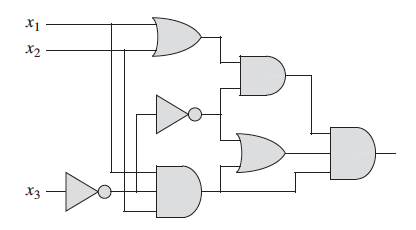
\includegraphics{Cormen_34_8.png}

I have labeled each of the logic gates, going left to right and top to bottom.  

\

\begin{tabular}{>{$}l<{$}}
	a = \lnot x_3 \cr
	b = x_1 \lor x_2 \cr
	c = \lnot a = x_3 \cr
	d = x_1 \land a \land x_2 = x_1 \land x_2 \land \lnot x_3 \cr
	e = b \land c = (x_1 \lor x_2) \land x_3 \cr
	f = c \lor d = x_3 \lor (x_1 \land x_2 \land \lnot x_3) = (x_1 \land x_2) \lor x_3 \cr
	g = e \land f \land d = ((x_1 \lor x_2) \land x_3) \land ((x_1 \land x_2) \lor x_3) \land (x_1 \land x_2 \land \lnot x_3) = (x_1 \land x_2) \land (x_3 \land \lnot x_3) \cr
\end{tabular}

\vskip 12pt

To test all of the inputs, we have $2^n$ inputs, where $n$ is the number of boolean variables.  Then we run each of those inputs through $k$ tests, where $k$ is the number of logic gates.  So we have $k\cdot 2^n$ tests, meaning that testing all of the inputs is $O(2^n)$.  

\

\begin{tabular}{*{12}{>{$}c<{$}|}}
	&&& a & b & c & d & e & f & g \cr
	x_1 & x_2 & x_3 & \lnot x_3 & x_1 \lor x_2 & \lnot a & x_1 \land a \land x_2 & b \land c & c \lor d & d \land e \land f \cr\hline
	0 & 0 & 0 & 1 & 0 & 0 & 0 & 0 & 0 & 0   \cr
	0 & 0 & 1 & 0 & 0 & 1 & 0 & 0 & 1 & 0   \cr
	0 & 1 & 0 & 1 & 1 & 0 & 0 & 0 & 0 & 0   \cr
	0 & 1 & 1 & 0 & 1 & 1 & 0 & 1 & 1 & 0   \cr
	1 & 0 & 0 & 1 & 1 & 0 & 0 & 0 & 0 & 0   \cr
	1 & 0 & 1 & 0 & 1 & 1 & 0 & 1 & 1 & 0   \cr
	1 & 1 & 0 & 1 & 1 & 0 & 1 & 0 & 1 & 0   \cr
	1 & 1 & 1 & 0 & 1 & 1 & 0 & 1 & 1 & 0  \cr
	
\end{tabular}

\

Direct method:  The problem is not satisfiable because we tested each of the instances and all of them failed.  

\

Heuristic (?) method:  The problem is not satisfiable because $d \land e = (x_1 \land x_2 \land \lnot x_3) \land ((x_1 \lor x_2) \land x_3) = x_1 \land (x_1 \lor x_2) \land x_2 \land x_3 \land \lnot x_3$, which depends on $x_3 \land \lnot x_3$ being true, which it is not for either value of $x_3$.  


\begin{lemma}
	The circuit-satisfiability problem belongs to NP.
\end{lemma}

\begin{proof}
	To ``belong to NP'' means to be verifiable in polynomial time.  We will give a sketch of a polynomial-time algorithm to verify an instance of the problem.  
	
	Two-input polynomial-time algorithm, $A$. 
	
	One input is a boolean combinational circuit, $C$  
	
	Second input is a {\it certificate} corresponding to an assignment of boolean values to the wires in the circuit $C$.
	
	  For each logic gate in $C$, the algorithm $A$ checks that the values of the output wire(s) are correctly computed from the values of the input wire(s).  If all of the computations are correct and the output of the entire circuit is 1, then the algorithm outputs 1.  Otherwise, (if any of the computations are incorrect, or if the output of the entire circuit is 0), then the algorithm $A$ returns 0.  
	  
	  For a satisfiable circuit $C$, there exists a certificate whose length is polynomial in the size of $C$ and that causes $A$ to output 1.   [Actually, the length of the certificate doesn't need to be larger than $C$.]  For an unsatisfiable circuit $C$, no certificate will return 1.  
	  
	  Since $A$ runs in (no worse than) polynomial time, we can verify the circuit satisfiability problem, so it belongs to NP.   
\end{proof}

\begin{lemma}
	The circuit-satisfiability problem is NP-hard.
\end{lemma}

\begin{proof}
	(To Do?)
\end{proof}

\begin{theorem}
	The circuit-satisfiability problem is NP-complete.
\end{theorem}

\begin{proof}
	Since the problem is both NP and NP-hard, by definition it is therefore NP-complete.
\end{proof}

\subsubsection{3-CNF or 3-P SAT}

A {\it literal} is an occurrence of a variable or its negation.  A boolean formula is in {\it conjunctive normal form} if it is expressed as an AND of clauses, each of which is an OR of one or more literals.  A boolean formula is in {\it 3-conjunctive normal form} or {\it 3-CNF} if each clause has exactly three distinct literals.  

The 3-CNF-SAT problem asks whether a given boolean formula $\phi$ in 3-CNF is satisfiable.  

\begin{theorem}
	Satisfiability of boolean formulas in 3-conjunctive normal form is NP-complete.  
\end{theorem}

Sketch of proof.  Need to prove that 3-CNF-SAT $\in$ NP and 3-CNF-SAT $\in$ NP-hard.   

To show that 3-CNF-SAT $\in$ NP, we show that there is a polynomial-time algorithm, $A$, to verify an instance of the problem.  The algorithm $A$ has two inputs, the boolean combinational circuit $C$ and a certificate corresponding to an assignment of boolean values to the wires in $C$.  To verify, we need to check that, for each gate, the boolean values on the input wires give the result on the output wire, and that the value of the final output wire is 1.  This verification algorithm is $O(|C|)$, where $|C|$ is the number of wires plus the number of gates; therefore, we have a polynomial-time algorithm that verifies any instance of the problem; therefore, 3-CNF-SAT $\in$ NP.  

To show that 3-CNF-SAT $\in$ NP-hard, we will show that SAT $\le_p$ 3-CNF-SAT, where ``$\le_p$'' is the {\it polynomial-time reducibility relation}. We do that by showing that every boolean combinational circuit satisfactiability problem can be transformed in polynomial time into a 3-conjunctive normal form satisfiability problem.  A general SAT problem cannot take longer than 3-CNF-SAT problems, because if it did, you could transform it into a 3-CNF-SAT problem and solve it; therefore, SAT $\le_p$ 3-CNF-SAT, and since SAT $\in$ NP-Complete, we have 3-CNF-SAT $\in$ NP-hard.  

Since 3-CNF-SAT $\in$ NP and 3-CNF-SAT $\in$ NP-hard, 3-CNF-SAT $\in$ NP-Complete.  {\it Q.E.D.}

\subsubsection{Example on page 1082 of reduction algorithm from SAT to 3-CNF-SAT}

\begin{align*}
\phi &= ((x_1 \to x_2) \lor \lnot (( \lnot x_1 \leftrightarrow x_3) \lor x_4)) \land \lnot x_2\cr
\phi &= 
\underbrace{
	\underbrace{
		((  
			\underbrace{x_1 \to x_2}_{y_3 = x_1 \to x_2}
		) \lor
		\underbrace{\lnot (  
			\underbrace{( 
				\underbrace{\lnot x_1 \leftrightarrow x_3}_{y_6 = \lnot x_1 \leftrightarrow x_3}
				) \lor x_4}_{y_5 = y_6 \lor x_4}
			)}_{y_4 = \lnot y_5}
	}_{y_2 = y_3 \lor y_4}
		) \land \lnot x_2
}_{y_1 = y_2 \land \lnot x_2}
	\cr
\end{align*}

\

Binary Parse Tree

\

\begin{tikzpicture}[x=6mm, y=10mm]
	\node (A) at (0,0) {$\phi$};
	\node [circle, draw, label=above right:$y_1$] (B) at (0,-1) {$\land$};
	\node [circle, draw, label=above right:$y_2$] (C) at (-8,-2) {$\lor$};
	\node [] (D) at (8,-2) {$\lnot x_2$};
	\node [circle, draw, label=above right:$y_3$] (E) at (-12,-3) {$\to$};
	\node [circle, draw, label=above right:$y_4$] (F) at (-4,-3) {$\lnot$};
	\node [] (G) at (-14,-4) {$x_1$};
	\node [] (H) at (-10,-4) {$x_2$};
	\node [circle, draw, label=above right:$y_5$] (I) at (-4,-4) {$\lor$};
	\node [circle, draw, label=above left:$y_6$] (J) at (-6,-5) {$\leftrightarrow$};
	\node [] (K) at (-2,-5) {$x_4$};
	\node [] (L) at (-7,-6) {$\lnot x_1$};
	\node [] (M) at (-5,-6) {$x_3$};
	
	\foreach \from/\to in {A/B, B/C, B/D, C/E, C/F, E/G, E/H, F/I, I/J, I/K, J/L, J/M}
		\draw (\from) -- (\to);
\end{tikzpicture}

\

\begin{tabular}{ *{10}{ >{$}c<{$}| } }
	&&&& y_3 & y_6 & y_5 & y_4 & y_2 & y_1 \cr
	x_1 & x_2 & x_3 & x_4 
		& x_1 \to x_2 
		& \lnot x_1 \leftrightarrow x_3 
		& y_6 \lor x_4 
		& \lnot y_5
		& y_3 \lor y_4 
		& y_2 \land \lnot x_2
	\cr\hline 
	0 & 0 & 0 & 0 & 1 & 0 & 0 & 1 & 1 & 1 \cr
	0 & 0 & 0 & 1 & 1 & 0 & 1 & 0 & 1 & 1 \cr  
	0 & 0 & 1 & 0 & 1 & 1 & 1 & 0 & 1 & 1 \cr  
	0 & 0 & 1 & 1 & 1 & 1 & 1 & 0 & 1 & 1 \cr  
	0 & 1 & 0 & 0 & 1 & 0 & 0 & 1 & 1 & 0 \cr  
	0 & 1 & 0 & 1 & 1 & 0 & 1 & 0 & 1 & 0 \cr  
	0 & 1 & 1 & 0 & 1 & 1 & 1 & 0 & 1 & 0 \cr  
	0 & 1 & 1 & 1 & 1 & 1 & 1 & 0 & 1 & 0 \cr  
	1 & 0 & 0 & 0 & 0 & 1 & 1 & 0 & 0 & 0 \cr  
	1 & 0 & 0 & 1 & 0 & 1 & 1 & 0 & 0 & 0 \cr  
	1 & 0 & 1 & 0 & 0 & 0 & 0 & 1 & 1 & 1 \cr  
	1 & 0 & 1 & 1 & 0 & 0 & 1 & 0 & 0 & 0 \cr  
	1 & 1 & 0 & 0 & 1 & 1 & 1 & 0 & 1 & 0 \cr  
	1 & 1 & 0 & 1 & 1 & 1 & 1 & 0 & 1 & 0 \cr  
	1 & 1 & 1 & 0 & 1 & 0 & 0 & 1 & 1 & 0 \cr  
	1 & 1 & 1 & 1 & 1 & 0 & 1 & 0 & 1 & 0 \cr  
\end{tabular}

\

See \verb|Reduction_1082.py|

\

We can rewrite a logical function $f$ on $a$ and $b$, $f(a,b)$, by introducing a variable $y$ that has the same value as $f(a,b)$, {\it i.e.} $y$ is true when $f(a,b)$ is true and $y$ is false when $f(a,b)$ is false.  They have the same value when $y \leftrightarrow f(a,b)$ is true.  We know that $f(a,b)$ is true when $y \land (y \leftrightarrow f(a,b))$ is true.  We can chain these together to get a formula $\phi'$ equivalent to $\phi$, as a conjunction of clauses $\phi'_i$ with at most three literals.  

\begin{align*}
	\phi' = y_1 &\land (y_1 \leftrightarrow (y_2 \land \lnot x_2)) \cr
		& \land (y_2 \leftrightarrow( y_3 \lor y_4 )) \cr
		& \land (y_3 \leftrightarrow( x_1 \to x_2 )) \cr
		& \land (y_4 \leftrightarrow( \lnot y_5 )) \cr
		& \land (y_5 \leftrightarrow( y_6 \lor x_4 )) \cr
		& \land (y_6 \leftrightarrow( \lnot x_1 \leftrightarrow x_3 )) \cr
\end{align*}

Below are the rows of the truth table for which $\phi' = 1$.  Note that they are the same values for $x_i$ as in $\phi$.  

\

\begin{tabular}{ *{12}{ |>{$}c<{$} } }
x_1 & x_2 & x_3 & x_4 & y_1 & y_2 & y_3 & y_4 & y_5 & y_6 & \phi' \cr\hline
0 & 0 & 0 & 0 & 1 & 1 & 1 & 1 & 0 & 0 & 1 &  \cr
0 & 0 & 0 & 1 & 1 & 1 & 1 & 0 & 1 & 0 & 1 &  \cr
0 & 0 & 1 & 0 & 1 & 1 & 1 & 0 & 1 & 1 & 1 &  \cr
0 & 0 & 1 & 1 & 1 & 1 & 1 & 0 & 1 & 1 & 1 &  \cr
1 & 0 & 1 & 0 & 1 & 1 & 0 & 1 & 0 & 0 & 1 &  \cr\end{tabular}

\

Now we have a formula $\phi'$ that is a conjunction of clauses $\phi'_i$, each of which has at least three literals.  To be in 3-conjunctive normal form, we need it to be a conjunction of clauses, each of which is a disjunction of exactly three literals.  To go from $\phi'$ to $\phi''$, follow these steps.  

\begin{enumerate}
	\item Make a truth table for each clause $\phi_i'$.  
	\item Using each entry that evaluates to 0, build a formula in disjunctive normal for (an OR of ANDs) that is equivalent to $\lnot \phi_i'$.
	\item Negate this formula and convert it into a CNF formula $\phi_i''$ using DeMorgan's laws for propositional logic, particularly that $\lnot (a \land b) = \lnot a \land \lnot b$ to complement all literals, changing ORs to ANDs and vice versa.  Now we have converted each clause $\phi_i'$ into a conjunctive normal form $\phi_i''$ with at most three literals.  
	\item If a clause $\phi_i''$ has fewer than three literals, pad it.  
	\item Take the conjunction of all of the clauses.  
\end{enumerate}

\begin{tabular}{*9{|>{$}c<{$}}}
	x_2 & y_1 & y_2 & y_2 \land \lnot x_2 & y_1 \leftrightarrow (y_2 \land \lnot x_2) & \text{DNF for } \lnot \phi_2' &  \text{CNF for } \phi_2'' \cr\hline
	1  & 1 & 1 & 0 & 0 & x_2 \land y_1 \land y_2 & \lnot x_2 \lor \lnot y_1 \lor \lnot y_2 \cr
	1  & 1 & 0 & 0 & 0 & x_2 \land y_1 \land \lnot y_2  & \lnot x_2 \lor \lnot y_1 \lor y_2  \cr
	1  & 0 & 1 & 0 & 1 && \cr
	1  & 0 & 0 & 0 & 1 && \cr
	0  & 1 & 1 & 1 & 1 && \cr
	0  & 1 & 0 & 0 & 0 & \lnot x_2 \land y_1 \land \lnot y_2  & x_2 \lor \lnot y_1 \lor  y_2  \cr
	0  & 0 & 1 & 1 & 0 & \lnot x_2 \land \lnot y_1 \land y_2  & x_2 \lor y_1 \lor \lnot y_2  \cr
	0  & 0 & 0 & 0 & 1 && \cr
\end{tabular}

$$\text{CNF:} \qquad \phi_2'' =  (\lnot x_2 \lor \lnot y_1 \lor \lnot y_2) \land ( \lnot x_2 \lor \lnot y_1 \lor y_2  ) \land (x_2 \lor \lnot y_1 \lor  y_2 ) \land ( x_2 \lor y_1 \lor \lnot y_2  )$$

\begin{tabular}{*9{|>{$}c<{$}}}
	x_2 & y_1 & y_2 & 
	\lnot x_2 \lor \lnot y_1 \lor \lnot y_2 &
	\lnot x_2 \lor \lnot y_1 \lor y_2 &
	x_2 \lor \lnot y_1 \lor  y_2 &
	x_2 \lor y_1 \lor \lnot y_2 & \phi_2'' \cr\hline
	1 & 1 & 1 & 0 & 1 & 1 & 1 & 0 \cr
	1 & 1 & 0 & 1 & 0 & 1 & 1 & 0 \cr
	1 & 0 & 1 & 1 & 1 & 1 & 1 & 1 \cr
	1 & 0 & 0 & 1 & 1 & 1 & 1 & 1 \cr
	0 & 1 & 1 & 1 & 1 & 1 & 1 & 1 \cr
	0 & 1 & 0 & 1 & 1 & 0 & 1 & 0 \cr
	0 & 0 & 1 & 1 & 1 & 1 & 0 & 0 \cr
	0 & 0 & 0 & 1 & 1 & 1 & 1 & 1 \cr
\end{tabular}

\

$\phi_5'$ has only two literals.  

\

\begin{tabular}{*9{|>{$}c<{$}}}
	y_4 & y_5 & y_4 \leftrightarrow \lnot y_5 & \lnot \phi_5' & \phi_5'' & \text{CNF for } \phi_5'' \cr\hline
	1 & 1 & 1 &  &  & \cr
	1 & 0 & 0 &  y_4 \land \lnot y_5 & \lnot y_4 \lor y_5 & (\lnot y_4 \lor y_5 \lor p) \land (\lnot y_4 \lor y_5 \lor \lnot p) \cr
	0 & 1 & 0 &  \lnot y_4 \land y_5 &y_4 \lor \lnot y_5  & (y_4 \lor \lnot y_5 \lor p) \land (y_4 \lor \lnot y_5 \lor \lnot p) \cr
	0 & 0 & 1 &  &  & \cr
\end{tabular}

$$\phi_5'' =  (\lnot y_4 \lor y_5 \lor p) \land (\lnot y_4 \lor y_5 \lor \lnot p) \land  (y_4 \lor \lnot y_5 \lor p) \land (y_4 \lor \lnot y_5 \lor \lnot p)  $$

\

$\phi_1'$ has only one literal.  

\

\begin{tabular}{*9{|>{$}c<{$}}}
	y_1 & \lnot \phi_1' & \phi_1'' & {\text CNF for } \phi_1'' \cr\hline
	1 &  && \cr
	0 & \lnot y_1 & y_1 & (y_1 \lor p \lor q) \land (y_1 \lor p \lor \lnot q) \land (y_1 \lor \lnot p \lor q) \land (y_1 \lor \lnot p \lor \lnot q)  \cr
\end{tabular}

\

This $p,q$ thing might make more sense if we put it in the table.  

\

\begin{tabular}{*9{|>{$}c<{$}}}
 	y_1 & p & q & y_1 & \lnot \phi_1' & \text{CNF for } \phi_1'' \cr\hline
 	1 & 1 & 1 & 1 &  &  \cr
 	1 & 1 & 0 & 1 &  &  \cr
 	1 & 0 & 1 & 1 &  &  \cr
 	1 & 0 & 0 & 1 &  &  \cr
 	0 & 1 & 1 & 0 & \lnot y_1 \land p \land q & y_1 \lor \lnot p \lor \lnot q \cr
 	0 & 1 & 0 & 0 & \lnot y_1 \land p \land \lnot q & y_1 \lor \lnot p \lor q  \cr
 	0 & 0 & 1 & 0 & \lnot y_1 \land \lnot p \land q  & y_1 \lor p \lor \lnot q  \cr
 	0 & 0 & 0 & 0 & \lnot y_1 \land \lnot p \land \lnot q  & y_1 \lor p \lor q  \cr
\end{tabular}

\

This conversion to 3-CNF takes polynomial time, so we have a polynomial-time reduction from SAT to 3-CNF-SAT; therefore, 3-CNF-SAT is at least as hard as SAT.  Since SAT is NP-complete and SAT $\le_p$ 3-CNF-SAT, we have 3-CNF-SAT is NP-complete.  

\subsubsection{2-CNF-SAT}

A 2-CNF is boolean formula in conjunctive normal form with exactly two literals per clause, like $(a \lor b) \land (\lnot a \lor b) \land (a \lor c)$.  

The interesting thing about 2-CNF is that $a \lor b \equiv \lnot a \to b \equiv \lnot b \to a$.  Use the pairs of implications to make an implication graph, a directed graph that is skew symmetric (if you swap the negations

A 2-CNF formula is satisfiable if and only if there is no variable that belongs to the same strongly connected component as its negation.  

To show that a boolean expression in 2-conjunctive normal form is satisfiable, 

\begin{enumerate}
	\item Write as an implication graph. 
	\item Use DFS or Kosaraju's algorithm to find the strongly connected components.  
	\item Check whether any strongly-connected component contains both a variable and its negation.  
\end{enumerate}

Each of these steps can be done in polynomial time, so the whole process can be done in polynomial time, so 2-CNF-SAT $\in$ P.

%%%%%
\subsection{Traveling Salesman Problem}

\subsubsection{TSP as a decision problem}

\begin{tabular}{lll}
	TSP = &$\{ (G, c, k)$: 
		& $G = (V,E)$ is a complete graph. \cr
		&& $c$ is a cost function from $V \times V \to \mathbb{N}$ \cr
		&& $k \in \mathbb{N}$, and \cr
		&& $G$ has a traveling-salesman tour with cost at most $k$. \cr
		&\} \cr
\end{tabular}

\

The traveling-salesman tour is a Hamiltonian cycle, visiting each node exactly once and returning to the starting point.  

To show that TSP $\in$ NP-complete, (a) show that TSP $\in$ P by walking through what it would take to confirm a solution and saying that it can be done in polynomial time, and (b) show that HAM-CYCLE $\le_P$ TSP by saying that HAM-CYCLE is a special case of TSP.  Since HAM-CYCLE is NP-complete, TSP is also.  

Let $G = (V,E)$ be an instance of HAM-CYCLE.  Form a complete graph $G' = (V, E')$ where $E' = \{(i,j): i,j \in V \text{ and } i \ne j\}$.  Define the cost function by $c(i,j) = 0 \text{ if } (i,j) \in E, 0 \text{ if } (i,j) \notin E$.  The instance of TSP is $(G', c, 0)$.  

The graph $G$ is a hamiltonian cycle iff graph $G'$ has a tour of cost at most 0.  

\subsubsection{Triangle Inequality}

If the cost function has the property that cutting out an intermediate stop never increases the cost, {\it i.e.} the most direct path between two points is not more expensive than a meandering one, {\it i.e.} the triangle inequality holds on the cost function, $c(u,w) \le c(u,v) + c(v,w)$, the problem is still NP-complete, but we can use Prim's algorithm for a minimal spanning tree to find, in polynomial time, an approximate solution whose total cost is no more than twice the optimal solution.  

%%%
\subsubsection{	S19 \#S6}
Many problem have been proved to be NP-complete.  To prove NP-completeness, it is necessary in general to demonstrate two proof components.  What are the two proof components to show a problem being NP-complete?
	
	Being NP-complete, the traveling-salesman problem (TSP) has a 2-approximation solution in polynomial time based on establishing a minimum spanning tree (MST) rooted at the start/end vertex (in polynomial time following MST-PRIM), if the graph edge weights observe the triangle inequality.  Sketch a brief proof to demonstrate that that such a proof satisfies 2-approximation.  



%%%%%
\subsection{Knapsack Problem}

%%%
\subsubsection{	S18 \#L4}
\begin{enumerate}[label=\alph*.]
		\item Define the following classes of a decision problem:  P, NP, and NP-completeness.
		\item Consider the 0-1 knapsack problem with $n$ objects each with its respective pre-defined profit.  The objective is to maximize the total profit that can be accommodated into a container of capacity $W$.  Define appropriate notations for weight and profit of objects, formulate the problem.
		\item Convert of the problem that you have defined in (b) into a decision problem.
		\item Show the problem that you have defined in (c) belongs to NP-class.
		\item Does the problem in (d) belong to the P-class or NP-completeness. (Justify your answer.)
		\item If principle of optimality be applicable to solve the problem defined in (c), formulate it.  Otherwise, explain why not.  
		\item What would be your explanation, if 0-1 knapsack problem is solved by dynamic programming in polynomial time?
\end{enumerate}

%%%%%
\subsection{Old Exam Problems}

%%%
\subsubsection{S15 \#L1}

\begin{enumerate}
		\item Suppose you have to find a solution to a problem that belongs to NP-complete class.  Clearly summarize the steps that will help you to find the solution of the problem.  
		\item John, an undergraduate student, recently took data structure course, states that heuristics algorithms always solve NP-complete problems.  He cites simplex methods as an example.  If you agree with John, justify why or why not.  
		\item What is the strategy behind a greedy algorithm?  Will it always provide an optimal solution?  If yes explain why, otherwise say why not.  
		\item Consider the following pseudo code for Kruskal's algorithm for solving minimal spanning tree (MST).

Algorithm MST.  Let $N$ be the number of nodes in graph $G$.  

\begin{lstlisting}[numbers=left, mathescape=True]
Sort the edges in non-decreasing order of cost.
$T$ is an empty graph
while $T$ has fewer than $N-1$ edges do:
	let $e$ denote the next edge of $G$ (in the order of cost)
	if $T \cup \{e\}$ does not contain a cycle, then $T = T \cup \{e\}$
\end{lstlisting}

Clearly mentioning the data structure you have to employ to reduce the time complexity to access and to maintain the necessary information, show the exact time taken to obtain the MST.  Also show the tight bound of the algorithm.  (Pay attention in detecting a cycle.)
\end{enumerate}

%%%
\subsubsection{Solutions}

1.  [From \S 35, page 1106]  There are three ways to approach an NP-Complete problem.  

a.  If the problem size is sufficiently small that, even if the growth is exponential or factorial, the time and resources required to solve it directly are within the time and money budgets, you may solve it directly.  

b.  See if the instances you are considering form a special case of the problem that can be solved in polynomial time.  

c.  Find an approximate solution.  

\

%%%
\subsubsection{S15 \#L3}

\begin{enumerate}
		\item Compare and contrast P, NP, NP-Complete, and NP-Hard.
		\item Based on current conjecture, draw a Venn diagram to show the relationship among these classes of problem.
		\item Clearly state what is understood by propositional satisfiability problem. 
		\item Suppose there are $m$ clauses and $k$ propositions in a given 3-p sat problem.  How many possible interpretations are there?  What is the time complexity of testing the satisfiability of a given interpretation?  What is the time and space complexity of testing the satisfiability of the clauses?
		\item Suppose you came across a research paper that highlights a clever heuristic strategy that the authors have used to solve an instance of 3-p sat which has 10,000 propositions and 10,000 clauses with 3 propositions.  They have generated several instances of the similar compositions of variables and clauses.  The authors, in their point of view, have demonstrated the power of their heuristic to solve an instance of NP-complete problem in polynomial time (empirically shown).  What would be your insight of their findings?
\end{enumerate}

\subsubsection{Solutions}

\begin{enumerate}
	\item 
	
\begin{description}
	\item [P] Solvable in polynomial time
	\item [NP] Verifiable in polynomial time
	\item [NP-Complete] Verifiable in polynomial time and at least as hard to solve as any other problem in NP
	\item [NP-Hard] At least as hard to solve as any other problem in NP, but not necessarily verifiable in polynomial time.  
\end{description}	

	$\text{P} \subset \text{NP}$
	
	$\text{NP-Complete} \subset \text{NP}$

	$\text{NP-Complete} \subset \text{NP-Hard}$
	
	$\text{NP-Complete} = \text{NP} \cap \text{NP-Hard}$
	
	The open question is whether there are problems verifiable in polynomial time that are not solvable in polynomial time.  

	\item \

\begin{tikzpicture}[x=10mm, y=5mm]
	\draw (0,0) ellipse (4 and 2); 
	\node () at (-0.5,0) {NP};
	\draw (5,0) ellipse (4 and 2);
	\node () at (6.5,0) {NP-Hard};
	\draw (-3,0) circle (1) node {P};
	\node () at (2.5,0) {NP-Complete};
\end{tikzpicture}

	% #3
	\item A propositional satisfiability problem asks, given a boolean combinational circuit composed of some number of inputs, AND, OR, and NOT gates, and single output, is there a set of inputs that will yield a TRUE (1) output? 

\end{enumerate}

%%%
\subsubsection{F15 \#S5}
Mark True or False for each of the following statements.  
\begin{enumerate}[label=\alph*.]
		\item Greedy strategy sometimes finds the best or the optimal solution.
		\item Dynamic programming will always find the optimal solution even when the principal of optimality condition is not satisfied.
		\item (Same as S5 \#S9b) Breadth first search is a special case of heuristic search algorithm.
		\item Some problems that belong to NP-class can be solved polynomially.  
		\item Satisfiability problem of propositional calculus is NP-complete.
\end{enumerate}

\subsubsection{Solutions}

\begin{enumerate}[label=\alph*.]
	\item
	\item
	\item
	\item  True.  Being NP means they can be verified in polynomial time.  It does not mean they cannot be solved in polynomial time.  
	\item  True.  There are some special cases, like 2-CNF, but in general, SAT is NP-complete.
\end{enumerate}

%%%
\subsubsection{F16 \#S5}

Suppose there are $n$ clauses and $m$ variables (propositions) in a given $3-p$ sat problem.
\begin{itemize}
	\item How many possible interpretations are there?
	\item Find the tight bound of checking for satisfiability of the $n$ clauses.  
\end{itemize}

%%%
\subsubsection{F16 \#L1}

\begin{enumerate}
	\item Briefly describe NP-class, P-class, NP-complete, and NP-hard.
	\item Show the conjectured relationship among the classes NP-class, P-class, NP-complete, and NP-hard.
	\item Show that counting $n$ objects with integer key values belongs to NP-class.  
	\item Provide the steps involved in showing whether a problem belongs to NP-complete or not.
	\item Illustrate the steps in step d by showing 3 proposition satisfiability (3-p sat) problem belongs to NP-complete.
	\item Provide a pseudo code that attempt to solve 3-p sat problem heuristically.
\end{enumerate}

%%%
\subsubsection{S17 \#L2}
\begin{enumerate}[label=\alph*.]
		\item Compare and contrast P, NP, NP-complete, and NP-hard.
		\item Based on current conjecture, draw a Venn diagram to show the relationship among these classes of problem.
		\item Suppose there $n$ clauses and $m$ propositions in a given 3p-sat problem.  How many possible interpretations are there?  What is the time complexity of testing the satisfiability of a given interpretation?  What is the time and space complexity of testing the satisfiability of the clauses?
		\item 3-p sat problem is NP-complete, but people still have published papers by applying heuristics strategy and showing that they were able to solve it with large number of distinct propositions (say 100) and large number of clauses (say 200).  To avoid any bias, they have generated the clauses and the set of propositions randomly.  How would you start investigating their results?  Can their results be generalized?
		\item Suppose a single NP-complete problem is solved in polynomial algorithm, what can you state about the entire NP-complete class as well as the NP-hard class.
\end{enumerate}

\subsubsection{Solutions}

\begin{enumerate}[label=\alph*.]
	% a.
	\item
	\begin{description}
		\item [P]  Solvable in polynomial time.  $O(n^k)$ for constant $k$.  
		\item [NP] Verifiable in polynomial time.  May or may not be solvable in polynomial time.  
		\item [NP-complete] Verifiable in polynomial time, but at least as hard to solve as any problem in NP.  Conjectured to not have a polynomial-time solution.  
		\item [NP-hard]  Both verification and solution are as hard as for any problem in NP.   Not known to be verifiable or solvable in polynomial time.  Conjectured to have polynomial-time methods for neither verification nor solution.  
	\end{description}
	
	P $\subset$ NP
	
	NP-complete $\subset$ NP
	
	NP-complete = NP $\cap$ NP-hard
	
	% b.
	\item \
	
\begin{tikzpicture}[x=10mm, y=5mm]
	\draw (0,0) ellipse (4 and 2); 
	\node () at (-0.5,0) {NP};
	\draw (5,0) ellipse (4 and 2);
	\node () at (6.5,0) {NP-Hard};
	\draw (-3,0) circle (1) node {P};
	\node () at (2.5,0) {NP-Complete};
\end{tikzpicture}

	% c.
	\item  I assume by ``number of propositions'' they mean ``number of propositional variables'' or ``number of variables.''  I don't find this topic in the textbook.  
	
	The number of interpretations (instances?) is $2^m$.  
	
	The truth table has $2^m$ rows and $m+n+1$ columns.  The first $m$ columns are just loop assignment.  The next $n$ columns evaluate the 3-disjunction clauses, each of which should take constant time.  The last column evaluates the conjunction of the $n$ clauses for each instance, which should take time proportional to the number $n$ of clauses.  
		
	So setting up and evaluating each row (interpretation, instance) should take $O(m+n+n) = O(m+n)$.  Since $m/2 \le n$, we can write that as $O(n)$.  Since there are $2^m$ rows, our total time is $O(n \cdot 2^n)$.  The memory required for testing the satisfiability of a clause is also $O(n)$.  
	
	
	
	% d.
	\item
	
	% e.
	\item A problem is NP-complete if it is at least as difficult as every problem in NP, {\it i.e.} a problem $A$ is NP-complete if, for every problem $B \in$ NP, there is a polynomial-time transformation $f$ such that any instance $\beta \in B$ can be transformed into an instance of $A$, so that $f(\beta) = \alpha \in A$.  The problem $A$ is at least as hard as $B$ because, if it were easier, we could use the solution method for $A$ to solve $B$.  
	
	 If a single NP-complete problem, like $A$, is solved in polynomial time, then each problem $B \in $ NP could be solved in polynomial time by transforming (in polynomial time) each instance of $B$ into an instance of $A$.  Thus, if one NP-complete problem could be solved in polynomial time, each and every NP problem (including each NP-complete problems) could be solved in polynomial time.  
	 
	 Finding a polynomial-time solution to an NP-complete problem would have no similar effect on the NP-hard problems that are not NP.  The definition of NP-hard says that each of those problems is at least as hard as each of the NP problems, but does not specify that it is at least as hard as any other NP-hard problems.  Taking down one does not make the group fall.  
	
\end{enumerate}

%%%
\subsubsection{	S18 \#L4}
\begin{enumerate}[label=\alph*.]
		\item Define the following classes of a decision problem:  P, NP, and NP-completeness.
		\item Consider the 0-1 knapsack problem with $n$ objects each with its respective pre-defined profit.  The objective is to maximize the total profit that can be accommodated into a container of capacity $W$.  Define appropriate notations for weight and profit of objects, formulate the problem.
		\item Convert of the problem that you have defined in (b) into a decision problem.
		\item Show the problem that you have defined in (c) belongs to NP-class.
		\item Does the problem in (d) belong to the P-class or NP-completeness. (Justify your answer.)
		\item If principle of optimality be applicable to solve the problem defined in (c), formulate it.  Otherwise, explain why not.  
		\item What would be your explanation, if 0-1 knapsack problem is solved by dynamic programming in polynomial time?
\end{enumerate}

\subsubsection{Solutions}

\begin{enumerate}[label=\alph*.]
	\item 
	\begin{description}
		\item [P] Solvable in polynomial time
		\item [NP] Verifiable in polynomial time
		\item [NP-complete] Verifiable in polynomial time, but at least as hard to solve as any other problem in NP.  Conjectured to not have a solution in polynomial time.  
	\end{description}
	
	P $\subset$ NP, NP-complete $\subset$ NP.
	
\end{enumerate}

%%%
\subsubsection{	S19 \#S6}
Many problem have been proved to be NP-complete.  To prove NP-completeness, it is necessary in general to demonstrate two proof components.  What are the two proof components to show a problem being NP-complete?
	
	Being NP-complete, the traveling-salesman problem (TSP) has a 2-approximation solution in polynomial time based on establishing a minimum spanning tree (MST) rooted at the start/end vertex (in polynomial time following MST-PRIM), if the graph edge weights observe the triangle inequality.  Sketch a brief proof to demonstrate that that such a proof satisfies 2-approximation.  

\subsubsection{Solution}

\begin{description}
	\item [First Part]
	
	NP-complete problems are the intersection of two sets, NP problems and NP hard problems.  To prove that a problem is NP-complete, we show that it belongs to both sets.  
	
	To prove that a problem is NP-complete, there are two steps.  First, we show that it is NP, meaning that a solution can be verified in polynomial time.  Second, we show that it is NP-hard, meaning that it is at least as hard to solve as a known (or conjectured) NP-hard problem.  
	
	\item [Second Part]
\end{description}


% Algorithms_Comp_TSP

\section{Traveling Salesman Problem}

\subsection{With the Triangle Inequality}

\begin{enumerate}
	\item Use MST-Prim to find a minimal spanning tree, $T$.  
	\item Make a list, $H$, of the vertices in the order in which they were first visited.
	\item This Hamiltonian cycle has cost no more than twice the cost of the optimal cycle.
	\item Since MST-Prim is $O(V^2)$, this method is a polynomial-time 2-approximation algorithm. 
\end{enumerate}

\subsection{Old Exam Problems}

\subsubsection{Spring 2019, \#S6}

Many problem have been proved to be NP-complete.  To prove NP-completeness, it is necessary in general to demonstrate two proof components.  What are the two proof components to show a problem being NP-complete?
	
	Being NP-complete, the traveling-salesman problem (TSP) has a 2-approximation solution in polynomial time based on establishing a minimum spanning tree (MST) rooted at the start/end vertex (in polynomial time following MST-PRIM), if the graph edge weights observe the triangle inequality.  Sketch a brief proof to demonstrate that that such a proof satisfies 2-approximation.  

\subsubsection{Solution to Second Part}

\begin{enumerate}
	\item Let $H*$ denote an optimal tour, and $c(H*)$ be the total cost of the edges of $H*$.  
	\item We obtained the spanning tree $T$ by deleting an edge from any tour, so $c(T) \le c(H*)$.  
	\item A full walk, $W$, of $T$ traverses each edge of $T$ exactly twice, so $c(W) = 2 c(T)$, so $c(W) \le 2c(H*)$.  
	\item The full walk, $W$, may not be a tour, because it may visit a vertex more than once.  Deleting a vertex from the walk does not increase its cost, because of the triangle inequality.  If we delete the second (or later) appearance of a vertex from the walk, we get the preorder walk of the tree $T$.  
	\item Let $H$ be the cycle corresponding to the preorder walk. It is Hamiltonian, because the each vertex appears in the preorder walk exactly once.  Since $c(H) \le c(W)$, we get $c(H) \le 2 c(H*)$; therefore, the method satisfies 2-approximation.   
\end{enumerate}



% Graph Algorithms
\chapter{Graph Algorithms}
\section{Graph Algorithms Summary}

\begin{tabular}{>{$}l<{$} l p{4in} }
	O(V+E) & BFS & Breadth First Search, finds distance from source to each node in an unweighted graph, directed or undirected.  Each vertex has a color, a distance, and a parent.  \cr
	O(V+E) & DFS & Depth First Search on an unweighted graph.  Each vertex has a color, a discovery time, a finishing time, and a parent.  Depth First Tree has tree edges, forward edges, back edges, and cross edges.  Used for topological sort.  \cr
	O(V^2), O(E \lg V) & Dijkstra & Finds shortest distance from the source in a weighted graph (directed or undirected).  Time complexity depends on the data structure we use for the queue.  \cr
\end{tabular}
\section{Breadth First Search and Depth First Search (BFS and DFS)}


\subsection{Old Exam Questions}

\subsubsection{Spring 2015 \#S9}	
	% S15 \#S9
	Mark true/false against the following statements. 
	\begin{enumerate}
		\item (Same as F15 \#S7a) A binary search tree of size $N$ will always find a key in at most $O(\log N)$ time.
		\item (Same as F15 \#S5c) A breadth first search algorithm can be considered as a special case of heuristic search algorithm.
		\item An optimal binary search tree is not necessarily a balanced tree.
		\item A dynamic programming approach uses top-down problem solving strategy to solve optimization problem.
	\end{enumerate}
	
\subsubsection{Solutions}

\begin{enumerate}
	\item Yes.  $\log N = h$, the height of the tree.  
	\item No. (?  The textbook doesn't talk about heuristics.)
	\item An {\it optimal binary search tree} is a tree whose expected cost is least.  We compute the expected cost using the (probability of searching for each node) $\times$ (depth of that node).  
	
	A {\it balanced tree} is one such that no two leaves differ in height by more than one.  
	
	I think the answer is ``No,"  because an optimal binary search tree has to be weight-balanced, not height-balanced.  
	\item No.  Dynamic programming uses bottom-up.  
\end{enumerate}

\subsubsection{Spring 2019 \#S5}
	% S19 S5
	BFS (breadth-first search) and DFS (depth-first search):  Give the visited node order for each type of graph search, starting with $S$ below.  

\
	
\hfil	\begin{tikzpicture}[x=20mm, y=10mm]
		\node [circle, draw] (S) at (0,0) {$S$};
		\node [circle, draw] (A) at (2,0) {$A$};
		\node [circle, draw] (B) at (3,-1) {$B$};
		\node [circle, draw] (C) at (2,-2) {$C$};
		\node [circle, draw] (D) at (0,-2) {$D$};
		\draw [-triangle 60] (S) -- (A);
		\draw [-triangle 60] (S) -- (D);
		\draw [-triangle 60] (A) -- (B);
		\draw [-triangle 60] (B) -- (C);
		\draw [-triangle 60] (C) -- (S);
		\draw [-triangle 60] (C) -- (A);
		\draw [-triangle 60] (D) -- (C);
	\end{tikzpicture}
	
\subsubsection{Solution} \

BFS:  $SADBC$ or $SDACB$, depending on the order in which the vertices are listed in $V$.  

\

Method for $V = \{S, A, B, C, D\}$, giving visited node order $SADBC$.

\

\hfil	\begin{tikzpicture}[x=15mm, y=10mm]
		\node [circle, draw, label=above:$S$, fill=gray] (S) at (0,0) {$0$};
		\node [circle, draw, label=above:$A$] (A) at (2,0) {$\infty$};
		\node [circle, draw, label=right:$B$] (B) at (3,-1) {$\infty$};
		\node [circle, draw, label=below:$C$] (C) at (2,-2) {$\infty$};
		\node [circle, draw, label=below:$D$] (D) at (0,-2) {$\infty$};
		\draw [-triangle 60] (S) -- (A);
		\draw [-triangle 60] (S) -- (D);
		\draw [-triangle 60] (A) -- (B);
		\draw [-triangle 60] (B) -- (C);
		\draw [-triangle 60] (C) -- (S);
		\draw [-triangle 60] (C) -- (A);
		\draw [-triangle 60] (D) -- (C);
		\node [below right] () at (4,1) {$Q = \{S\}$};
		\node [below right] () at (4,0) {
			\begin{tabular}{>{$}c<{$}|*6{>{$}c<{$}}}
				 u & S & A & B & C & D \cr\hline
				 u.color & Gray & White & White & White & White \cr
				 u.d & 0 & \infty & \infty & \infty & \infty \cr
				 u.\pi & NIL & NIL & NIL & NIL & NIL \cr
			\end{tabular}
		};
	\end{tikzpicture}
	
\hfil	\begin{tikzpicture}[x=15mm, y=10mm]
		\node [circle, draw, label=above:$S$, fill=black] (S) at (0,0) {\color{white}$0$};
		\node [circle, draw, label=above:$A$, fill=gray] (A) at (2,0) {$1$};
		\node [circle, draw, label=right:$B$] (B) at (3,-1) {$\infty$};
		\node [circle, draw, label=below:$C$] (C) at (2,-2) {$\infty$};
		\node [circle, draw, label=below:$D$, fill=gray] (D) at (0,-2) {$1$};
		\draw [-triangle 60] (S) -- (A);
		\draw [-triangle 60] (S) -- (D);
		\draw [-triangle 60] (A) -- (B);
		\draw [-triangle 60] (B) -- (C);
		\draw [-triangle 60] (C) -- (S);
		\draw [-triangle 60] (C) -- (A);
		\draw [-triangle 60] (D) -- (C);
		\node [below right] () at (4,1) {$Q = \{A, D\}$};
		\node [below right] () at (4,0) {
			\begin{tabular}{>{$}c<{$}|*6{>{$}c<{$}}}
				 u & S & A & B & C & D \cr\hline
				 u.color & Black & Gray & White & White & Gray \cr
				 u.d & 0 & 1 & \infty & \infty & 1 \cr
				 u.\pi & NIL & S & NIL & NIL & S \cr
			\end{tabular}
		};
	\end{tikzpicture}
	
\hfil	\begin{tikzpicture}[x=15mm, y=10mm]
		\node [circle, draw, label=above:$S$, fill=black] (S) at (0,0) {\color{white}$0$};
		\node [circle, draw, label=above:$A$, fill=black] (A) at (2,0) {\color{white}$1$};
		\node [circle, draw, label=right:$B$, fill=gray] (B) at (3,-1) {$2$};
		\node [circle, draw, label=below:$C$] (C) at (2,-2) {$\infty$};
		\node [circle, draw, label=below:$D$, fill=gray] (D) at (0,-2) {$1$};
		\draw [-triangle 60] (S) -- (A);
		\draw [-triangle 60] (S) -- (D);
		\draw [-triangle 60] (A) -- (B);
		\draw [-triangle 60] (B) -- (C);
		\draw [-triangle 60] (C) -- (S);
		\draw [-triangle 60] (C) -- (A);
		\draw [-triangle 60] (D) -- (C);
		\node [below right] () at (4,1) {$Q = \{D, B\}$};
		\node [below right] () at (4,0) {
			\begin{tabular}{>{$}c<{$}|*6{>{$}c<{$}}}
				 u & S & A & B & C & D \cr\hline
				 u.color & Black & Black & Gray & White & Gray \cr
				 u.d & 0 & 1 & 2 & \infty & 1 \cr
				 u.\pi & NIL & S & A & NIL & S \cr
			\end{tabular}
		};
	\end{tikzpicture}
	
\hfil	\begin{tikzpicture}[x=15mm, y=10mm]
		\node [circle, draw, label=above:$S$, fill=black] (S) at (0,0) {\color{white}$0$};
		\node [circle, draw, label=above:$A$, fill=black] (A) at (2,0) {\color{white}$1$};
		\node [circle, draw, label=right:$B$, fill=gray] (B) at (3,-1) {$2$};
		\node [circle, draw, label=below:$C$, fill=gray] (C) at (2,-2) {$2$};
		\node [circle, draw, label=below:$D$, fill=black] (D) at (0,-2) {$\color{white}1$};
		\draw [-triangle 60] (S) -- (A);
		\draw [-triangle 60] (S) -- (D);
		\draw [-triangle 60] (A) -- (B);
		\draw [-triangle 60] (B) -- (C);
		\draw [-triangle 60] (C) -- (S);
		\draw [-triangle 60] (C) -- (A);
		\draw [-triangle 60] (D) -- (C);
		\node [below right] () at (4,1) {$Q = \{B, C\}$};
		\node [below right] () at (4,0) {
			\begin{tabular}{>{$}c<{$}|*6{>{$}c<{$}}}
				 u & S & A & B & C & D \cr\hline
				 u.color & Black & Black & Gray & Gray & Black \cr
				 u.d & 0 & 1 & 2 & 2 & 1 \cr
				 u.\pi & NIL & S & A & D & S \cr
			\end{tabular}
		};
	\end{tikzpicture}
	
\hfil	\begin{tikzpicture}[x=15mm, y=10mm]
		\node [circle, draw, label=above:$S$, fill=black] (S) at (0,0) {\color{white}$0$};
		\node [circle, draw, label=above:$A$, fill=black] (A) at (2,0) {\color{white}$1$};
		\node [circle, draw, label=right:$B$, fill=black] (B) at (3,-1) {\color{white}$2$};
		\node [circle, draw, label=below:$C$, fill=gray] (C) at (2,-2) {$2$};
		\node [circle, draw, label=below:$D$, fill=black] (D) at (0,-2) {$\color{white}1$};
		\draw [-triangle 60] (S) -- (A);
		\draw [-triangle 60] (S) -- (D);
		\draw [-triangle 60] (A) -- (B);
		\draw [-triangle 60] (B) -- (C);
		\draw [-triangle 60] (C) -- (S);
		\draw [-triangle 60] (C) -- (A);
		\draw [-triangle 60] (D) -- (C);
		\node [below right] () at (4,1) {$Q = \{C\}$};
		\node [below right] () at (4,0) {
			\begin{tabular}{>{$}c<{$}|*6{>{$}c<{$}}}
				 u & S & A & B & C & D \cr\hline
				 u.color & Black & Black & Gray & Gray & Black \cr
				 u.d & 0 & 1 & 2 & 2 & 1 \cr
				 u.\pi & NIL & S & A & D & S \cr
			\end{tabular}
		};
	\end{tikzpicture}
	
\hfil	\begin{tikzpicture}[x=15mm, y=10mm]
		\node [circle, draw, label=above:$S$, fill=black] (S) at (0,0) {\color{white}$0$};
		\node [circle, draw, label=above:$A$, fill=black] (A) at (2,0) {\color{white}$1$};
		\node [circle, draw, label=right:$B$, fill=black] (B) at (3,-1) {\color{white}$2$};
		\node [circle, draw, label=below:$C$, fill=black] (C) at (2,-2) {\color{white}$2$};
		\node [circle, draw, label=below:$D$, fill=black] (D) at (0,-2) {$\color{white}1$};
		\draw [-triangle 60] (S) -- (A);
		\draw [-triangle 60] (S) -- (D);
		\draw [-triangle 60] (A) -- (B);
		\draw [-triangle 60] (B) -- (C);
		\draw [-triangle 60] (C) -- (S);
		\draw [-triangle 60] (C) -- (A);
		\draw [-triangle 60] (D) -- (C);
		\node [below right] () at (4,1) {$Q = \{\}$};
		\node [below right] () at (4,0) {
			\begin{tabular}{>{$}c<{$}|*6{>{$}c<{$}}}
				 u & S & A & B & C & D \cr\hline
				 u.color & Black & Black & Gray & Gray & Black \cr
				 u.d & 0 & 1 & 2 & 2 & 1 \cr
				 u.\pi & NIL & S & A & D & S \cr
			\end{tabular}
		};
	\end{tikzpicture}
	
\

DFS:  $SABCD$ or $SDCAB$, depending on the order of $V$.  

\

$V = \{S, A, B, C, D\}$

\

\hfil	\begin{tikzpicture}[x=15mm, y=10mm]
		\node [circle, draw, label=above:$S$, fill=gray] (S) at (0,0) {$1$};
		\node [circle, draw, label=above:$A$] (A) at (2,0) { \ };
		\node [circle, draw, label=right:$B$] (B) at (3,-1) { \ };
		\node [circle, draw, label=below:$C$] (C) at (2,-2) { \ };
		\node [circle, draw, label=below:$D$] (D) at (0,-2) { \ };
		\draw [-triangle 60] (S) -- (A);
		\draw [-triangle 60] (S) -- (D);
		\draw [-triangle 60] (A) -- (B);
		\draw [-triangle 60] (B) -- (C);
		\draw [-triangle 60] (C) -- (S);
		\draw [-triangle 60] (C) -- (A);
		\draw [-triangle 60] (D) -- (C);
		\node [below right] () at (4,1) {DFS-Visit ($G,S$),   $time = 1$};
		\node [below right] () at (4,0) {
			\begin{tabular}{>{$}c<{$}|*6{>{$}c<{$}}}
				 u & S & A & B & C & D \cr\hline
				 u.color & Gray & White & White & White & White \cr
				 u.d & 1 &  \cr
				 u.f & \cr
				 u.\pi & NIL & S & NIL & NIL & NIL \cr
			\end{tabular}
		};
	\end{tikzpicture}
	

\

\hfil	\begin{tikzpicture}[x=15mm, y=10mm]
		\node [circle, draw, label=above:$S$, fill=gray] (S) at (0,0) {1};
		\node [circle, draw, label=above:$A$, fill=gray] (A) at (2,0) {2};
		\node [circle, draw, label=right:$B$] (B) at (3,-1) { \ };
		\node [circle, draw, label=below:$C$] (C) at (2,-2) { \ };
		\node [circle, draw, label=below:$D$] (D) at (0,-2) { \ };
		\draw [-triangle 60] (S) -- (A);
		\draw [-triangle 60] (S) -- (D);
		\draw [-triangle 60] (A) -- (B);
		\draw [-triangle 60] (B) -- (C);
		\draw [-triangle 60] (C) -- (S);
		\draw [-triangle 60] (C) -- (A);
		\draw [-triangle 60] (D) -- (C);
		\node [below right] () at (4,1) {DFS-Visit ($G,A$),   $time = 2$};
		\node [below right] () at (4,0) {
			\begin{tabular}{>{$}c<{$}|*6{>{$}c<{$}}}
				 u & S & A & B & C & D \cr\hline
				 u.color & Gray & Gray & White & White & White \cr
				 u.d & 1 & 2 \cr
				 u.f & \cr
				 u.\pi & NIL & S & A & NIL & NIL \cr
			\end{tabular}
		};
	\end{tikzpicture}
	
\

\hfil	\begin{tikzpicture}[x=15mm, y=10mm]
		\node [circle, draw, label=above:$S$, fill=gray] (S) at (0,0) {1};
		\node [circle, draw, label=above:$A$, fill=gray] (A) at (2,0) {2};
		\node [circle, draw, label=right:$B$, fill=gray] (B) at (3,-1) {3};
		\node [circle, draw, label=below:$C$] (C) at (2,-2) { \ };
		\node [circle, draw, label=below:$D$] (D) at (0,-2) { \ };
		\draw [-triangle 60] (S) -- (A);
		\draw [-triangle 60] (S) -- (D);
		\draw [-triangle 60] (A) -- (B);
		\draw [-triangle 60] (B) -- (C);
		\draw [-triangle 60] (C) -- (S);
		\draw [-triangle 60] (C) -- (A);
		\draw [-triangle 60] (D) -- (C);
		\node [below right] () at (4,1) {DFS-Visit ($G,B$),   $time = 3$};
		\node [below right] () at (4,0) {
			\begin{tabular}{>{$}c<{$}|*6{>{$}c<{$}}}
				 u & S & A & B & C & D \cr\hline
				 u.color & Gray & Gray & Gray & White & White \cr
				 u.d & 1 & 2 & 3 \cr
				 u.f & \cr
				 u.\pi & NIL & S & A & B & NIL \cr
			\end{tabular}
		};
	\end{tikzpicture}
	
	
\

\hfil	\begin{tikzpicture}[x=15mm, y=10mm]
		\node [circle, draw, label=above:$S$, fill=gray] (S) at (0,0) {1};
		\node [circle, draw, label=above:$A$, fill=gray] (A) at (2,0) {2};
		\node [circle, draw, label=right:$B$, fill=gray] (B) at (3,-1) {3};
		\node [circle, draw, label=below:$C$, fill=gray] (C) at (2,-2) {4};
		\node [circle, draw, label=below:$D$] (D) at (0,-2) { \ };
		\draw [-triangle 60] (S) -- (A);
		\draw [-triangle 60] (S) -- (D);
		\draw [-triangle 60] (A) -- (B);
		\draw [-triangle 60] (B) -- (C);
		\draw [-triangle 60] (C) -- (S);
		\draw [-triangle 60] (C) -- (A);
		\draw [-triangle 60] (D) -- (C);
		\node [below right] () at (4,1) {First part of DFS-Visit ($G,C$),   $time = 4$};
		\node [below right] () at (4,0) {
			\begin{tabular}{>{$}c<{$}|*6{>{$}c<{$}}}
				 u & S & A & B & C & D \cr\hline
				 u.color & Gray & Gray & Gray & Gray & White \cr
				 u.d & 1 & 2 & 3 & 4 \cr
				 u.f & \cr
				 u.\pi & NIL & S & A & B & NIL \cr
			\end{tabular}
		};
	\end{tikzpicture}
	
\

\hfil	\begin{tikzpicture}[x=15mm, y=10mm]
		\node [circle, draw, label=above:$S$, fill=gray] (S) at (0,0) {1};
		\node [circle, draw, label=above:$A$, fill=gray] (A) at (2,0) {2};
		\node [circle, draw, label=right:$B$, fill=gray] (B) at (3,-1) {3};
		\node [circle, draw, label=below:$C$, fill=black] (C) at (2,-2) {\color{white}4/5};
		\node [circle, draw, label=below:$D$] (D) at (0,-2) { \ };
		\draw [-triangle 60] (S) -- (A);
		\draw [-triangle 60] (S) -- (D);
		\draw [-triangle 60] (A) -- (B);
		\draw [-triangle 60] (B) -- (C);
		\draw [-triangle 60] (C) -- (S);
		\draw [-triangle 60] (C) -- (A);
		\draw [-triangle 60] (D) -- (C);
		\node [below right] () at (4,1) {Second part of DFS-Visit ($G,C$),   $time = 5$};
		\node [below right] () at (4,0) {
			\begin{tabular}{>{$}c<{$}|*6{>{$}c<{$}}}
				 u & S & A & B & C & D \cr\hline
				 u.color & Gray & Gray & Gray & Black & White \cr
				 u.d & 1 & 2 & 3 & 4 \cr
				 u.f & & & & 5\cr
				 u.\pi & NIL & S & A & B & NIL \cr
			\end{tabular}
		};
	\end{tikzpicture}
	
	
\

\hfil	\begin{tikzpicture}[x=15mm, y=10mm]
		\node [circle, draw, label=above:$S$, fill=gray] (S) at (0,0) {1};
		\node [circle, draw, label=above:$A$, fill=gray] (A) at (2,0) {2};
		\node [circle, draw, label=right:$B$, fill=black] (B) at (3,-1) {\color{white}3/6};
		\node [circle, draw, label=below:$C$, fill=black] (C) at (2,-2) {\color{white}4/5};
		\node [circle, draw, label=below:$D$] (D) at (0,-2) { \ };
		\draw [-triangle 60] (S) -- (A);
		\draw [-triangle 60] (S) -- (D);
		\draw [-triangle 60] (A) -- (B);
		\draw [-triangle 60] (B) -- (C);
		\draw [-triangle 60] (C) -- (S);
		\draw [-triangle 60] (C) -- (A);
		\draw [-triangle 60] (D) -- (C);
		\node [below right] () at (4,1) {Back to second part of DFS-Visit ($G,B$),   $time = 6$};
		\node [below right] () at (4,0) {
			\begin{tabular}{>{$}c<{$}|*6{>{$}c<{$}}}
				 u & S & A & B & C & D \cr\hline
				 u.color & Gray & Gray & Black & Black & White \cr
				 u.d & 1 & 2 & 3 & 4 \cr
				 u.f & & & 6 & 5\cr
				 u.\pi & NIL & S & A & B & NIL \cr
			\end{tabular}
		};
	\end{tikzpicture}
	
\

\hfil	\begin{tikzpicture}[x=15mm, y=10mm]
		\node [circle, draw, label=above:$S$, fill=gray] (S) at (0,0) {1};
		\node [circle, draw, label=above:$A$, fill=black] (A) at (2,0) {\color{white}2/7};
		\node [circle, draw, label=right:$B$, fill=black] (B) at (3,-1) {\color{white}3/6};
		\node [circle, draw, label=below:$C$, fill=black] (C) at (2,-2) {\color{white}4/5};
		\node [circle, draw, label=below:$D$] (D) at (0,-2) { \ };
		\draw [-triangle 60] (S) -- (A);
		\draw [-triangle 60] (S) -- (D);
		\draw [-triangle 60] (A) -- (B);
		\draw [-triangle 60] (B) -- (C);
		\draw [-triangle 60] (C) -- (S);
		\draw [-triangle 60] (C) -- (A);
		\draw [-triangle 60] (D) -- (C);
		\node [below right] () at (4,1) {Back to second part of DFS-Visit ($G,A$),   $time = 7$};
		\node [below right] () at (4,0) {
			\begin{tabular}{>{$}c<{$}|*6{>{$}c<{$}}}
				 u & S & A & B & C & D \cr\hline
				 u.color & Gray & Black & Black & Black & White \cr
				 u.d & 1 & 2 & 3 & 4 \cr
				 u.f & & 7 & 6 & 5\cr
				 u.\pi & NIL & S & A & B & NIL \cr
			\end{tabular}
		};
	\end{tikzpicture}
	
	
\

\hfil	\begin{tikzpicture}[x=15mm, y=10mm]
		\node [circle, draw, label=above:$S$, fill=gray] (S) at (0,0) {1};
		\node [circle, draw, label=above:$A$, fill=black] (A) at (2,0) {\color{white}2/7};
		\node [circle, draw, label=right:$B$, fill=black] (B) at (3,-1) {\color{white}3/6};
		\node [circle, draw, label=below:$C$, fill=black] (C) at (2,-2) {\color{white}4/5};
		\node [circle, draw, label=below:$D$] (D) at (0,-2) { \ };
		\draw [-triangle 60] (S) -- (A);
		\draw [-triangle 60] (S) -- (D);
		\draw [-triangle 60] (A) -- (B);
		\draw [-triangle 60] (B) -- (C);
		\draw [-triangle 60] (C) -- (S);
		\draw [-triangle 60] (C) -- (A);
		\draw [-triangle 60] (D) -- (C);
		\node [below right] () at (4,1) {Back to {\tt for} loop in DFS-Visit ($G,S$),   $time = 7$};
		\node [below right] () at (4,0) {
			\begin{tabular}{>{$}c<{$}|*6{>{$}c<{$}}}
				 u & S & A & B & C & D \cr\hline
				 u.color & Gray & Black & Black & Black & White \cr
				 u.d & 1 & 2 & 3 & 4 & \cr
				 u.f & & 7 & 6 & 5\cr
				 u.\pi & NIL & S & A & B & S \cr
			\end{tabular}
		};
	\end{tikzpicture}
	
	
\

\hfil	\begin{tikzpicture}[x=15mm, y=10mm]
		\node [circle, draw, label=above:$S$, fill=gray] (S) at (0,0) {1};
		\node [circle, draw, label=above:$A$, fill=black] (A) at (2,0) {\color{white}2/7};
		\node [circle, draw, label=right:$B$, fill=black] (B) at (3,-1) {\color{white}3/6};
		\node [circle, draw, label=below:$C$, fill=black] (C) at (2,-2) {\color{white}4/5};
		\node [circle, draw, label=below:$D$, fill=gray] (D) at (0,-2) {8};
		\draw [-triangle 60] (S) -- (A);
		\draw [-triangle 60] (S) -- (D);
		\draw [-triangle 60] (A) -- (B);
		\draw [-triangle 60] (B) -- (C);
		\draw [-triangle 60] (C) -- (S);
		\draw [-triangle 60] (C) -- (A);
		\draw [-triangle 60] (D) -- (C);
		\node [below right] () at (4,1) {First part of DFS-Visit ($G,D$),   $time = 8$};
		\node [below right] () at (4,0) {
			\begin{tabular}{>{$}c<{$}|*6{>{$}c<{$}}}
				 u & S & A & B & C & D \cr\hline
				 u.color & Gray & Black & Black & Black & Gray \cr
				 u.d & 1 & 2 & 3 & 4 & 8 \cr
				 u.f & & 7 & 6 & 5\cr
				 u.\pi & NIL & S & A & B & S \cr
			\end{tabular}
		};
	\end{tikzpicture}
	
\

\hfil	\begin{tikzpicture}[x=15mm, y=10mm]
		\node [circle, draw, label=above:$S$, fill=gray] (S) at (0,0) {1};
		\node [circle, draw, label=above:$A$, fill=black] (A) at (2,0) {\color{white}2/7};
		\node [circle, draw, label=right:$B$, fill=black] (B) at (3,-1) {\color{white}3/6};
		\node [circle, draw, label=below:$C$, fill=black] (C) at (2,-2) {\color{white}4/5};
		\node [circle, draw, label=below:$D$, fill=black] (D) at (0,-2) {\color{white}8/9};
		\draw [-triangle 60] (S) -- (A);
		\draw [-triangle 60] (S) -- (D);
		\draw [-triangle 60] (A) -- (B);
		\draw [-triangle 60] (B) -- (C);
		\draw [-triangle 60] (C) -- (S);
		\draw [-triangle 60] (C) -- (A);
		\draw [-triangle 60] (D) -- (C);
		\node [below right] () at (4,1) {Second part of DFS-Visit ($G,D$),   $time = 9$};
		\node [below right] () at (4,0) {
			\begin{tabular}{>{$}c<{$}|*6{>{$}c<{$}}}
				 u & S & A & B & C & D \cr\hline
				 u.color & Gray & Black & Black & Black & Black \cr
				 u.d & 1 & 2 & 3 & 4 & 8 \cr
				 u.f & & 7 & 6 & 5 & 9 \cr
				 u.\pi & NIL & S & A & B & S \cr
			\end{tabular}
		};
	\end{tikzpicture}
	
\

\hfil	\begin{tikzpicture}[x=15mm, y=10mm]
		\node [circle, draw, label=above:$S$, fill=black] (S) at (0,0) {\color{white}1/10};
		\node [circle, draw, label=above:$A$, fill=black] (A) at (2,0) {\color{white}2/7};
		\node [circle, draw, label=right:$B$, fill=black] (B) at (3,-1) {\color{white}3/6};
		\node [circle, draw, label=below:$C$, fill=black] (C) at (2,-2) {\color{white}4/5};
		\node [circle, draw, label=below:$D$, fill=black] (D) at (0,-2) {\color{white}8/9};
		\draw [-triangle 60] (S) -- (A);
		\draw [-triangle 60] (S) -- (D);
		\draw [-triangle 60] (A) -- (B);
		\draw [-triangle 60] (B) -- (C);
		\draw [-triangle 60] (C) -- (S);
		\draw [-triangle 60] (C) -- (A);
		\draw [-triangle 60] (D) -- (C);
		\node [below right] () at (4,1) {Second part of DFS-Visit ($G,S$),   $time = 10$};
		\node [below right] () at (4,0) {
			\begin{tabular}{>{$}c<{$}|*6{>{$}c<{$}}}
				 u & S & A & B & C & D \cr\hline
				 u.color & Gray & Black & Black & Black & Black \cr
				 u.d & 1 & 2 & 3 & 4 & 8 \cr
				 u.f & 10 & 7 & 6 & 5 & 9 \cr
				 u.\pi & NIL & S & A & B & S \cr
			\end{tabular}
		};
	\end{tikzpicture}
	





\subsubsection{Fall 2015 \#S5}


	% #F15 S5
	Mark True or False for each of the following statements.  
	
	\begin{enumerate}[label=\alph*.]
		\item Greedy strategy sometimes finds the best or the optimal solution.
		\item Dynamic programming will always find the optimal solution even when the principal of optimality condition is not satisfied.
		\item (Same as S5 \#S9b) Breadth first search is a special case of heuristic search algorithm.
		\item Some problems that belong to NP-class can be solved polynomially.  
		\item Satisfiability problem of propositional calculus is NP-complete.
	\end{enumerate}

\subsubsection{Solutions}

\begin{enumerate}[label=\alph*.]
	\item True.
	\item False.
	\item Don't know.  
	\item True.
	\item True.
\end{enumerate}

\subsubsection{Fall 2016 \#S8}

	% F16 #S8
	Mark true/false (T/F) against the following statements.  
	
	\begin{enumerate}
		\item A binary search tree of size $N$ will always find a key at most $O(\lg N)$ time
		\item A breadth first search can be considered as a special case of heuristic search algorithm.
		\item An optimal binary search tree is not necessarily being a balanced tree.
		\item A dynamic programming approach uses top-down problem solving strategy to solve optimization problem.
	\end{enumerate}
	
\subsubsection{Solutions}

\begin{enumerate}
	\item True
	\item Don't know.
	\item True.
	\item False.  
\end{enumerate}

\subsubsection{Fall 2018 \#L3}

	% F18 #L3
	Follow depth-first search (DFS), starting from Node $s$, to traverse the graph shown below, with its edge weights all ignored and the start time equal to 1.  Mark (1) the type of every edge and (2) the discovery and finish times of each node.
	
	Follow breadth-first search (BFS), starting from Node $s$, to traverse the graph shown below, with its edge weights all ignored.  Show the predecessor tree rooted at Node $s$ after BFS, with the number of links (i.e. distance) from Node $s$ to every other node indicated.  
	
	\
	
	\hfil \begin{tikzpicture}[x=15mm, y=15mm]
		\node [circle, draw, label=left:$s$] (s) at (0,0) {};
		\node [circle, draw, label=above:$t$] (t) at (1,1) {};
		\node [circle, draw, label=above:$x$] (x) at (3,1) {};
		\node [circle, draw, label=below:$y$] (y) at (1,-1) {};
		\node [circle, draw, label=below:$z$] (z) at (3,-1) {};
		\foreach \from/\to/\weight in {s/t/10, s/y/-8, t/x/1, y/x/9, y/z/2}
			\draw [-triangle 60] (\from) -- (\to) node [midway, rectangle, fill=white] {\weight};
		\foreach \from/\to/\weight in {z/s/7}
			\draw [-triangle 60] (\from) -- (\to) node [pos=0.3, rectangle, fill=white] {\weight};
		\foreach \from/\to/\weight in {t/y/2, y/t/3, x/z/-4, z/x/6}
			\draw [bend right=20, -triangle 60] (\from) to node [midway, rectangle, fill=white] {\weight} (\to);
			
	\end{tikzpicture}
	
\

[Note: If the edge weights aren't relevant, why did they leave them in the diagram?]

\subsubsection{DFS Solution}

There are four types of edges.  

\begin{description}
	\item [Tree edges] are edges in the depth-first forest $G_\pi$.  Edge $(u,v)$ is a tree edge if $v$ was first discovered by exploring edge $(u,v)$.  The tree edges below are in bold.  
	\item [Back edges] connect a vertex to an ancestor.  
	\item [Forward edges] are non-tree edges that connect a vertex to a descendent.
	\item [Cross edges] are everything else.  
\end{description}

\

	\hfil \begin{tikzpicture}[x=15mm, y=15mm]
		\node [circle, draw, label=left:$s$, fill=gray] (s) at (0,0) {\color{white}1};
		\node [circle, draw, label=above:$t$] (t) at (1,1) {\color{white}1};
		\node [circle, draw, label=above:$x$] (x) at (3,1) {\color{white}1};
		\node [circle, draw, label=below:$y$] (y) at (1,-1) {\color{white}1};
		\node [circle, draw, label=below:$z$] (z) at (3,-1) {\color{white}1};
		\foreach \from/\to in {s/t, s/y, t/x, y/x, y/z, z/s}
			\draw [-triangle 60] (\from) -- (\to);
		\foreach \from/\to/\weight in {}
			\draw [-triangle 60] (\from) -- (\to) node [midway, rectangle, fill=white] {\weight};
		\foreach \from/\to/\weight in {}
			\draw [-triangle 60] (\from) -- (\to) node [pos=0.3, rectangle, fill=white] {\weight};
		\foreach \from/\to in {t/y, y/t, x/z, z/x}
			\draw [bend right=20, -triangle 60] (\from) to (\to);
		\foreach \from/\to/\weight in {}
			\draw [bend right=20, -triangle 60] (\from) to node [midway, rectangle, fill=white] {\weight} (\to);
			
		\node [below right] () at (4,1) {
			\begin{tabular}{ >{$}l<{$} | *5{>{$}c<{$}} }
				c & s & t & x & y & z \cr\hline
				c.color & Gray & White & White & White & White \cr
				c.d  & 1 \cr
				c.f \cr
				c.\pi & NIL & NIL & NIL & NIL & NIL  \cr				
			\end{tabular}
		}; 
	\end{tikzpicture}
	
\

	\hfil \begin{tikzpicture}[x=15mm, y=15mm]
		\node [circle, draw, label=left:$s$, fill=gray] (s) at (0,0) {\color{white}1};
		\node [circle, draw, label=above:$t$, fill=gray] (t) at (1,1) {\color{white}2};
		\node [circle, draw, label=above:$x$] (x) at (3,1) {\color{white}1};
		\node [circle, draw, label=below:$y$] (y) at (1,-1) {\color{white}1};
		\node [circle, draw, label=below:$z$] (z) at (3,-1) {\color{white}1};
		\foreach \from/\to in {s/t, s/y, t/x, y/x, y/z, z/s}
			\draw [-triangle 60] (\from) -- (\to);
		\foreach \from/\to in {s/t}
			\draw [ultra thick, -triangle 60] (\from) -- (\to);
		\foreach \from/\to/\weight in {}
			\draw [-triangle 60] (\from) -- (\to) node [midway, rectangle, fill=white] {\weight};
		\foreach \from/\to/\weight in {}
			\draw [-triangle 60] (\from) -- (\to) node [pos=0.3, rectangle, fill=white] {\weight};
		\foreach \from/\to in {t/y, y/t, x/z, z/x}
			\draw [bend right=20, -triangle 60] (\from) to (\to);
		\foreach \from/\to/\weight in {}
			\draw [bend right=20, -triangle 60] (\from) to node [midway, rectangle, fill=white] {\weight} (\to);
			
		\node [below right] () at (4,1) {
			\begin{tabular}{ >{$}l<{$} | *5{>{$}c<{$}} }
				c & s & t & x & y & z \cr\hline
				c.color & Gray & Gray & White & White & White \cr
				c.d  & 1 & 2 \cr
				c.f \cr
				c.\pi & NIL & S & NIL & NIL & NIL  \cr				
			\end{tabular}
		}; 
	\end{tikzpicture}
	
\

	\hfil \begin{tikzpicture}[x=15mm, y=15mm]
		\node [circle, draw, label=left:$s$, fill=gray] (s) at (0,0) {\color{white}1};
		\node [circle, draw, label=above:$t$, fill=gray] (t) at (1,1) {\color{white}2};
		\node [circle, draw, label=above:$x$, fill=gray] (x) at (3,1) {\color{white}3};
		\node [circle, draw, label=below:$y$] (y) at (1,-1) {\color{white}1};
		\node [circle, draw, label=below:$z$] (z) at (3,-1) {\color{white}1};
		\foreach \from/\to in {s/t, s/y, t/x, y/x, y/z, z/s}
			\draw [-triangle 60] (\from) -- (\to);
		\foreach \from/\to in {s/t, t/x}
			\draw [ultra thick, -triangle 60] (\from) -- (\to);
		\foreach \from/\to/\weight in {}
			\draw [-triangle 60] (\from) -- (\to) node [midway, rectangle, fill=white] {\weight};
		\foreach \from/\to/\weight in {}
			\draw [-triangle 60] (\from) -- (\to) node [pos=0.3, rectangle, fill=white] {\weight};
		\foreach \from/\to in {t/y, y/t, x/z, z/x}
			\draw [bend right=20, -triangle 60] (\from) to (\to);
		\foreach \from/\to/\weight in {}
			\draw [bend right=20, -triangle 60] (\from) to node [midway, rectangle, fill=white] {\weight} (\to);
			
		\node [below right] () at (4,1) {
			\begin{tabular}{ >{$}l<{$} | *5{>{$}c<{$}} }
				c & s & t & x & y & z \cr\hline
				c.color & Gray & Gray & Gray & White & White \cr
				c.d  & 1 & 2 & 3 \cr
				c.f \cr
				c.\pi & NIL & s & t & NIL & NIL  \cr				
			\end{tabular}
		}; 
	\end{tikzpicture}
	
\

	\hfil \begin{tikzpicture}[x=15mm, y=15mm]
		\node [circle, draw, label=left:$s$, fill=gray] (s) at (0,0) {\color{white}1};
		\node [circle, draw, label=above:$t$, fill=gray] (t) at (1,1) {\color{white}2};
		\node [circle, draw, label=above:$x$, fill=gray] (x) at (3,1) {\color{white}3};
		\node [circle, draw, label=below:$y$] (y) at (1,-1) {\color{white}1};
		\node [circle, draw, label=below:$z$, fill=gray] (z) at (3,-1) {\color{white}4};
		\foreach \from/\to in {s/t, s/y, t/x, y/x, y/z, z/s}
			\draw [-triangle 60] (\from) -- (\to);
		\foreach \from/\to in {s/t, t/x}
			\draw [ultra thick, -triangle 60] (\from) -- (\to);
		\foreach \from/\to/\weight in {}
			\draw [-triangle 60] (\from) -- (\to) node [midway, rectangle, fill=white] {\weight};
		\foreach \from/\to/\weight in {}
			\draw [-triangle 60] (\from) -- (\to) node [pos=0.3, rectangle, fill=white] {\weight};
		\foreach \from/\to in {t/y, y/t, x/z, z/x}
			\draw [bend right=20, -triangle 60] (\from) to (\to);
		\foreach \from/\to in {x/z}
			\draw [ultra thick, bend right=20, -triangle 60] (\from) to (\to);
		\foreach \from/\to/\weight in {}
			\draw [bend right=20, -triangle 60] (\from) to node [midway, rectangle, fill=white] {\weight} (\to);
			
		\node [below right] () at (4,1) {
			\begin{tabular}{ >{$}l<{$} | *5{>{$}c<{$}} }
				c & s & t & x & y & z \cr\hline
				c.color & Gray & Gray & Gray & White & Gray \cr
				c.d  & 1 & 2 & 3 & & 4 \cr
				c.f \cr
				c.\pi & NIL & s & t & NIL & x  \cr				
			\end{tabular}
		}; 
	\end{tikzpicture}
	
\

	\hfil \begin{tikzpicture}[x=15mm, y=15mm]
		\node [circle, draw, label=left:$s$, fill=gray] (s) at (0,0) {\color{white}1};
		\node [circle, draw, label=above:$t$, fill=gray] (t) at (1,1) {\color{white}2};
		\node [circle, draw, label=above:$x$, fill=gray] (x) at (3,1) {\color{white}3};
		\node [circle, draw, label=below:$y$] (y) at (1,-1) {\color{white}1};
		\node [circle, draw, label=below:$z$, fill=black] (z) at (3,-1) {\color{white}4/5};
		\foreach \from/\to in {s/t, s/y, t/x, y/x, y/z}
			\draw [-triangle 60] (\from) -- (\to);
		\foreach \from/\to in {s/t, t/x}
			\draw [ultra thick, -triangle 60] (\from) -- (\to);
		\foreach \from/\to/\weight in {}
			\draw [-triangle 60] (\from) -- (\to) node [midway, rectangle, fill=white] {\weight};
		\foreach \from/\to/\weight in {z/s/back}
			\draw [-triangle 60] (\from) -- (\to) node [pos=0.3, rectangle, fill=white] {\weight};
		\foreach \from/\to in {t/y, y/t, x/z}
			\draw [bend right=20, -triangle 60] (\from) to (\to);
		\foreach \from/\to in {x/z}
			\draw [ultra thick, bend right=20, -triangle 60] (\from) to (\to);
		\foreach \from/\to/\weight in {z/x/back}
			\draw [bend right=20, -triangle 60] (\from) to node [midway, rectangle, fill=white] {\weight} (\to);
			
		\node [below right] () at (4,1) {
			\begin{tabular}{ >{$}l<{$} | *5{>{$}c<{$}} }
				c & s & t & x & y & z \cr\hline
				c.color & Gray & Gray & Gray & White & Black \cr
				c.d  & 1 & 2 & 3 & & 4 \cr
				c.f  & & & & & 5 \cr
				c.\pi & NIL & s & t & NIL & x  \cr				
			\end{tabular}
		}; 
	\end{tikzpicture}
	
\

	\hfil \begin{tikzpicture}[x=15mm, y=15mm]
		\node [circle, draw, label=left:$s$, fill=gray] (s) at (0,0) {\color{white}1};
		\node [circle, draw, label=above:$t$, fill=gray] (t) at (1,1) {\color{white}2};
		\node [circle, draw, label=above:$x$, fill=black] (x) at (3,1) {\color{white}3/6};
		\node [circle, draw, label=below:$y$] (y) at (1,-1) {\color{white}1};
		\node [circle, draw, label=below:$z$, fill=black] (z) at (3,-1) {\color{white}4/5};
		\foreach \from/\to in {s/t, s/y, t/x, y/x, y/z}
			\draw [-triangle 60] (\from) -- (\to);
		\foreach \from/\to in {s/t, t/x}
			\draw [ultra thick,-triangle 60] (\from) -- (\to);
		\foreach \from/\to/\weight in {}
			\draw [-triangle 60] (\from) -- (\to) node [midway, rectangle, fill=white] {\weight};
		\foreach \from/\to/\weight in {z/s/back}
			\draw [-triangle 60] (\from) -- (\to) node [pos=0.3, rectangle, fill=white] {\weight};

		\foreach \from/\to in {t/y, y/t, x/z}
			\draw [bend right=20, -triangle 60] (\from) to (\to);
		\foreach \from/\to in {x/z}
			\draw [ultra thick, bend right=20, -triangle 60] (\from) to (\to);
		\foreach \from/\to/\weight in {z/x/back}
			\draw [bend right=20, -triangle 60] (\from) to node [midway, rectangle, fill=white] {\weight} (\to);
			
		\node [below right] () at (4,1) {
			\begin{tabular}{ >{$}l<{$} | *5{>{$}c<{$}} }
				c & s & t & x & y & z \cr\hline
				c.color & Gray & Gray & Black & White & Black \cr
				c.d  & 1 & 2 & 3 & & 4 \cr
				c.f  &  & & 6 & & 5 \cr
				c.\pi & NIL & s & t & NIL & x  \cr				
			\end{tabular}
		}; 
	\end{tikzpicture}
	
\

	\hfil \begin{tikzpicture}[x=15mm, y=15mm]
		\node [circle, draw, label=left:$s$, fill=gray] (s) at (0,0) {\color{white}1};
		\node [circle, draw, label=above:$t$, fill=gray] (t) at (1,1) {\color{white}2};
		\node [circle, draw, label=above:$x$, fill=black] (x) at (3,1) {\color{white}3/6};
		\node [circle, draw, label=below:$y$, fill=gray] (y) at (1,-1) {\color{white}7};
		\node [circle, draw, label=below:$z$, fill=black] (z) at (3,-1) {\color{white}4/5};
		\foreach \from/\to in {s/t, s/y, t/x, y/x, y/z}
			\draw [-triangle 60] (\from) -- (\to);
		\foreach \from/\to in {s/t, t/x}
			\draw [ultra thick,-triangle 60] (\from) -- (\to);
		\foreach \from/\to/\weight in {}
			\draw [-triangle 60] (\from) -- (\to) node [midway, rectangle, fill=white] {\weight};
		\foreach \from/\to/\weight in {z/s/back}
			\draw [-triangle 60] (\from) -- (\to) node [pos=0.3, rectangle, fill=white] {\weight};

		\foreach \from/\to in {t/y, y/t, x/z}
			\draw [bend right=20, -triangle 60] (\from) to (\to);
		\foreach \from/\to in {x/z, t/y}
			\draw [ultra thick, bend right=20, -triangle 60] (\from) to (\to);
		\foreach \from/\to/\weight in {z/x/back}
			\draw [bend right=20, -triangle 60] (\from) to node [midway, rectangle, fill=white] {\weight} (\to);
			
		\node [below right] () at (4,1) {
			\begin{tabular}{ >{$}l<{$} | *5{>{$}c<{$}} }
				c & s & t & x & y & z \cr\hline
				c.color & Gray & Gray & Black & Gray & Black \cr
				c.d  & 1 & 2 & 3 & 7 & 4 \cr
				c.f  & &  & 6 & & 5 \cr
				c.\pi & NIL & s & t & t & x  \cr				
			\end{tabular}
		}; 
	\end{tikzpicture}
	
\

	\hfil \begin{tikzpicture}[x=15mm, y=15mm]
		\node [circle, draw, label=left:$s$, fill=gray] (s) at (0,0) {\color{white}1};
		\node [circle, draw, label=above:$t$, fill=gray] (t) at (1,1) {\color{white}2};
		\node [circle, draw, label=above:$x$, fill=black] (x) at (3,1) {\color{white}3/6};
		\node [circle, draw, label=below:$y$, fill=black] (y) at (1,-1) {\color{white}7/8};
		\node [circle, draw, label=below:$z$, fill=black] (z) at (3,-1) {\color{white}4/5};
		\foreach \from/\to in {s/t, s/y, t/x, y/x, y/z}
			\draw [-triangle 60] (\from) -- (\to);
		\foreach \from/\to in {s/t, t/x}
			\draw [ultra thick,-triangle 60] (\from) -- (\to);
		\foreach \from/\to/\weight in {y/x/cross, y/z/cross}
			\draw [-triangle 60] (\from) -- (\to) node [midway, rectangle, fill=white] {\weight};
		\foreach \from/\to/\weight in {z/s/back}
			\draw [-triangle 60] (\from) -- (\to) node [pos=0.3, rectangle, fill=white] {\weight};

		\foreach \from/\to in {t/y, y/t, x/z}
			\draw [bend right=20, -triangle 60] (\from) to (\to);
		\foreach \from/\to in {x/z, t/y}
			\draw [ultra thick, bend right=20, -triangle 60] (\from) to (\to);
		\foreach \from/\to/\weight in {z/x/back, y/t/back}
			\draw [bend right=20, -triangle 60] (\from) to node [midway, rectangle, fill=white] {\weight} (\to);
			
		\node [below right] () at (4,1) {
			\begin{tabular}{ >{$}l<{$} | *5{>{$}c<{$}} }
				c & s & t & x & y & z \cr\hline
				c.color & Gray & Gray & Black & Black & Black \cr
				c.d  & 1 & 2 & 3 & 7 & 4 \cr
				c.f  & &  & 6 & 8 & 5 \cr
				c.\pi & NIL & s & t & t & x  \cr				
			\end{tabular}
		}; 
	\end{tikzpicture}
	
\

	\hfil \begin{tikzpicture}[x=15mm, y=15mm]
		\node [circle, draw, label=left:$s$, fill=gray] (s) at (0,0) {\color{white}1};
		\node [circle, draw, label=above:$t$, fill=black] (t) at (1,1) {\color{white}2/9};
		\node [circle, draw, label=above:$x$, fill=black] (x) at (3,1) {\color{white}3/6};
		\node [circle, draw, label=below:$y$, fill=black] (y) at (1,-1) {\color{white}7/8};
		\node [circle, draw, label=below:$z$, fill=black] (z) at (3,-1) {\color{white}4/5};
		\foreach \from/\to in {s/t, s/y, t/x, y/x, y/z}
			\draw [-triangle 60] (\from) -- (\to);
		\foreach \from/\to in {s/t, t/x}
			\draw [ultra thick,-triangle 60] (\from) -- (\to);
		\foreach \from/\to/\weight in {y/x/cross, y/z/cross}
			\draw [-triangle 60] (\from) -- (\to) node [midway, rectangle, fill=white] {\weight};
		\foreach \from/\to/\weight in {z/s/back}
			\draw [-triangle 60] (\from) -- (\to) node [pos=0.3, rectangle, fill=white] {\weight};

		\foreach \from/\to in {t/y, y/t, x/z}
			\draw [bend right=20, -triangle 60] (\from) to (\to);
		\foreach \from/\to in {x/z, t/y}
			\draw [ultra thick, bend right=20, -triangle 60] (\from) to (\to);
		\foreach \from/\to/\weight in {z/x/back, y/t/back}
			\draw [bend right=20, -triangle 60] (\from) to node [midway, rectangle, fill=white] {\weight} (\to);
			
		\node [below right] () at (4,1) {
			\begin{tabular}{ >{$}l<{$} | *5{>{$}c<{$}} }
				c & s & t & x & y & z \cr\hline
				c.color & Gray & Black & Black & Black & Black \cr
				c.d  & 1 & 2 & 3 & 7 & 4 \cr
				c.f  & & 9 & 6 & 8 & 5 \cr
				c.\pi & NIL & s & t & t & x  \cr				
			\end{tabular}
		}; 
	\end{tikzpicture}
	
\

	\hfil \begin{tikzpicture}[x=15mm, y=15mm]
		\node [circle, draw, label=left:$s$, fill=black] (s) at (-1,0) {\color{white}1/10};
		\node [circle, draw, label=above:$t$, fill=black] (t) at (1,1) {\color{white}2/9};
		\node [circle, draw, label=above:$x$, fill=black] (x) at (3,1) {\color{white}3/6};
		\node [circle, draw, label=below:$y$, fill=black] (y) at (1,-1) {\color{white}7/8};
		\node [circle, draw, label=below:$z$, fill=black] (z) at (3,-1) {\color{white}4/5};
		\foreach \from/\to in {s/t, t/x, y/x, y/z}
			\draw [-triangle 60] (\from) -- (\to);
		\foreach \from/\to in {s/t, t/x}
			\draw [ultra thick,-triangle 60] (\from) -- (\to);
		\foreach \from/\to/\weight in {y/x/cross, y/z/cross, s/y/forward}
			\draw [-triangle 60] (\from) -- (\to) node [midway, rectangle, fill=white] {\weight};
		\foreach \from/\to/\weight in {z/s/back}
			\draw [-triangle 60] (\from) -- (\to) node [pos=0.3, rectangle, fill=white] {\weight};

		\foreach \from/\to in {t/y, y/t, x/z}
			\draw [bend right=20, -triangle 60] (\from) to (\to);
		\foreach \from/\to in {x/z, t/y}
			\draw [ultra thick, bend right=20, -triangle 60] (\from) to (\to);
		\foreach \from/\to/\weight in {z/x/back, y/t/back}
			\draw [bend right=20, -triangle 60] (\from) to node [midway, rectangle, fill=white] {\weight} (\to);
			
		\node [below right] () at (4,1) {
			\begin{tabular}{ >{$}l<{$} | *5{>{$}c<{$}} }
				c & s & t & x & y & z \cr\hline
				c.color & Black & Black & Black & Black & Black \cr
				c.d  & 1 & 2 & 3 & 7 & 4 \cr
				c.f  & 10 & 9 & 6 & 8 & 5 \cr
				c.\pi & NIL & s & t & t & x  \cr				
			\end{tabular}
		}; 
	\end{tikzpicture}
	
\

Depth First Tree

\

	\hfil \begin{tikzpicture}[x=25mm, y=25mm]
		\node [circle, draw, label=left:$s$, fill=black] (s) at (0,0) {\color{white}1/10};
		\node [circle, draw, label=below:$t$, fill=black] (t) at (0,-1) {\color{white}2/9};
		\node [circle, draw, label=above:$x$, fill=black] (x) at (1.5,-2) {\color{white}3/6};
		\node [circle, draw, label=below:$y$, fill=black] (y) at (-1,-2) {\color{white}7/8};
		\node [circle, draw, label=below:$z$, fill=black] (z) at (1,-3) {\color{white}4/5};
		\foreach \from/\to in {s/t, t/x, y/x, y/z}
			\draw [-triangle 60] (\from) -- (\to);
		\foreach \from/\to in {s/t, t/x}
			\draw [ultra thick,-triangle 60] (\from) -- (\to);
		\foreach \from/\to/\weight in {y/x/cross, y/z/cross, s/y/forward}
			\draw [-triangle 60] (\from) -- (\to) node [midway, rectangle, fill=white] {\weight};
		\foreach \from/\to/\weight in {z/s/back}
			\draw [-triangle 60] (\from) -- (\to) node [pos=0.7, right, rectangle, fill=white] {\weight};

		\foreach \from/\to in {t/y, y/t, x/z}
			\draw [bend right=20, -triangle 60] (\from) to (\to);
		\foreach \from/\to in {x/z, t/y}
			\draw [ultra thick, bend right=20, -triangle 60] (\from) to (\to);
		\foreach \from/\to/\weight in {z/x/back, y/t/back}
			\draw [bend right=20, -triangle 60] (\from) to node [midway, rectangle, fill=white] {\weight} (\to);
			
	\end{tikzpicture}
	
\

%%%%%%%%%%%%
\subsubsection{BFS Solution}

$V = \{s, t, x, y, z\}$

\

	\hfil \begin{tikzpicture}[x=15mm, y=15mm]
		\node [circle, draw, label=left:$s$, fill=gray] (s) at (0,0) {\color{white}0};
		\node [circle, draw, label=above:$t$] (t) at (1,1) {\color{white}1};
		\node [circle, draw, label=above:$x$] (x) at (3,1) {\color{white}1};
		\node [circle, draw, label=below:$y$] (y) at (1,-1) {\color{white}1};
		\node [circle, draw, label=below:$z$] (z) at (3,-1) {\color{white}1};
		\foreach \from/\to in {s/t, s/y, t/x, y/x, y/z, z/s}
			\draw [-triangle 60] (\from) -- (\to);
		\foreach \from/\to/\weight in {}
			\draw [-triangle 60] (\from) -- (\to) node [midway, rectangle, fill=white] {\weight};
		\foreach \from/\to/\weight in {}
			\draw [-triangle 60] (\from) -- (\to) node [pos=0.3, rectangle, fill=white] {\weight};
		\foreach \from/\to in {t/y, y/t, x/z, z/x}
			\draw [bend right=20, -triangle 60] (\from) to (\to);
		\foreach \from/\to/\weight in {}
			\draw [bend right=20, -triangle 60] (\from) to node [midway, rectangle, fill=white] {\weight} (\to);
				
		
		\node [below right] () at (4,1.5) {	$Q = \{s\}$};
			
		\node [below right] () at (4,1) {
			\begin{tabular}{ >{$}l<{$} | *5{>{$}c<{$}} }
				c & s & t & x & y & z \cr\hline
				c.color & Gray & White & White & White & White \cr
				c.d  & 0 \cr
				c.\pi & NIL & NIL & NIL & NIL & NIL  \cr				
			\end{tabular}
		}; 
	\end{tikzpicture}
	
\

	\hfil \begin{tikzpicture}[x=15mm, y=15mm]
		\node [circle, draw, label=left:$s$, fill=black] (s) at (0,0) {\color{white}0};
		\node [circle, draw, label=above:$t$, fill = gray] (t) at (1,1) {\color{white}1};
		\node [circle, draw, label=above:$x$] (x) at (3,1) {\color{white}1};
		\node [circle, draw, label=below:$y$, fill=gray] (y) at (1,-1) {\color{white}1};
		\node [circle, draw, label=below:$z$] (z) at (3,-1) {\color{white}1};

		\foreach \from/\to in {s/t, s/y, t/x, y/x, y/z, z/s}
			\draw [-triangle 60] (\from) -- (\to);
		\foreach \from/\to in {s/t, s/y}
			\draw [ultra thick,-triangle 60] (\from) -- (\to);

		\foreach \from/\to/\weight in {}
			\draw [-triangle 60] (\from) -- (\to) node [midway, rectangle, fill=white] {\weight};
		\foreach \from/\to/\weight in {}
			\draw [-triangle 60] (\from) -- (\to) node [pos=0.3, rectangle, fill=white] {\weight};
		\foreach \from/\to in {t/y, y/t, x/z, z/x}
			\draw [bend right=20, -triangle 60] (\from) to (\to);
		\foreach \from/\to/\weight in {}
			\draw [bend right=20, -triangle 60] (\from) to node [midway, rectangle, fill=white] {\weight} (\to);
				
		
		\node [below right] () at (4,1.5) {	$Q = \{t,y\}$};
			
		\node [below right] () at (4,1) {
			\begin{tabular}{ >{$}l<{$} | *5{>{$}c<{$}} }
				c & s & t & x & y & z \cr\hline
				c.color & Black & Gray & White & Gray & White \cr
				c.d  & 0 & 1 & & 1 &  \cr
				c.\pi & NIL & s & NIL & s & NIL  \cr				
			\end{tabular}
		}; 
	\end{tikzpicture}
	
\

	\hfil \begin{tikzpicture}[x=15mm, y=15mm]
		\node [circle, draw, label=left:$s$, fill=black] (s) at (0,0) {\color{white}0};
		\node [circle, draw, label=above:$t$, fill = black] (t) at (1,1) {\color{white}1};
		\node [circle, draw, label=above:$x$, fill=gray] (x) at (3,1) {\color{white}2};
		\node [circle, draw, label=below:$y$, fill=gray] (y) at (1,-1) {\color{white}1};
		\node [circle, draw, label=below:$z$] (z) at (3,-1) {\color{white}1};

		\foreach \from/\to in {s/t, s/y, t/x, y/x, y/z, z/s}
			\draw [-triangle 60] (\from) -- (\to);
		\foreach \from/\to in {s/t, s/y, t/x}
			\draw [ultra thick,-triangle 60] (\from) -- (\to);

		\foreach \from/\to/\weight in {}
			\draw [-triangle 60] (\from) -- (\to) node [midway, rectangle, fill=white] {\weight};
		\foreach \from/\to/\weight in {}
			\draw [-triangle 60] (\from) -- (\to) node [pos=0.3, rectangle, fill=white] {\weight};
		\foreach \from/\to in {t/y, y/t, x/z, z/x}
			\draw [bend right=20, -triangle 60] (\from) to (\to);
		\foreach \from/\to/\weight in {}
			\draw [bend right=20, -triangle 60] (\from) to node [midway, rectangle, fill=white] {\weight} (\to);
				
		
		\node [below right] () at (4,1.5) {	$Q = \{y, x\}$};
			
		\node [below right] () at (4,1) {
			\begin{tabular}{ >{$}l<{$} | *5{>{$}c<{$}} }
				c & s & t & x & y & z \cr\hline
				c.color & Black & Black & Gray & Gray & White \cr
				c.d  & 0 & 1 &2 & 1 &  \cr
				c.\pi & NIL & s & t & s & NIL  \cr				
			\end{tabular}
		}; 
	\end{tikzpicture}
	
\

	\hfil \begin{tikzpicture}[x=15mm, y=15mm]
		\node [circle, draw, label=left:$s$, fill=black] (s) at (0,0) {\color{white}0};
		\node [circle, draw, label=above:$t$, fill = black] (t) at (1,1) {\color{white}1};
		\node [circle, draw, label=above:$x$, fill=gray] (x) at (3,1) {\color{white}2};
		\node [circle, draw, label=below:$y$, fill=black] (y) at (1,-1) {\color{white}1};
		\node [circle, draw, label=below:$z$, fill=gray] (z) at (3,-1) {\color{white}3};

		\foreach \from/\to in {s/t, s/y, t/x, y/x, y/z, z/s}
			\draw [-triangle 60] (\from) -- (\to);
		\foreach \from/\to in {s/t, s/y, t/x, y/z}
			\draw [ultra thick,-triangle 60] (\from) -- (\to);

		\foreach \from/\to/\weight in {}
			\draw [-triangle 60] (\from) -- (\to) node [midway, rectangle, fill=white] {\weight};
		\foreach \from/\to/\weight in {}
			\draw [-triangle 60] (\from) -- (\to) node [pos=0.3, rectangle, fill=white] {\weight};
		\foreach \from/\to in {t/y, y/t, x/z, z/x}
			\draw [bend right=20, -triangle 60] (\from) to (\to);
		\foreach \from/\to/\weight in {}
			\draw [bend right=20, -triangle 60] (\from) to node [midway, rectangle, fill=white] {\weight} (\to);
				
		
		\node [below right] () at (4,1.5) {	$Q = \{x, z\}$};
			
		\node [below right] () at (4,1) {
			\begin{tabular}{ >{$}l<{$} | *5{>{$}c<{$}} }
				c & s & t & x & y & z \cr\hline
				c.color & Black & Black & Gray & Black & Gray \cr
				c.d  & 0 & 1 &2 & 1 & 3 \cr
				c.\pi & NIL & s & t & s & y  \cr				
			\end{tabular}
		}; 
	\end{tikzpicture}
	
\

	\hfil \begin{tikzpicture}[x=15mm, y=15mm]
		\node [circle, draw, label=left:$s$, fill=black] (s) at (0,0) {\color{white}0};
		\node [circle, draw, label=above:$t$, fill = black] (t) at (1,1) {\color{white}1};
		\node [circle, draw, label=above:$x$, fill=black] (x) at (3,1) {\color{white}2};
		\node [circle, draw, label=below:$y$, fill=black] (y) at (1,-1) {\color{white}1};
		\node [circle, draw, label=below:$z$, fill=gray] (z) at (3,-1) {\color{white}3};

		\foreach \from/\to in {s/t, s/y, t/x, y/x, y/z, z/s}
			\draw [-triangle 60] (\from) -- (\to);
		\foreach \from/\to in {s/t, s/y, t/x, y/z}
			\draw [ultra thick,-triangle 60] (\from) -- (\to);

		\foreach \from/\to/\weight in {}
			\draw [-triangle 60] (\from) -- (\to) node [midway, rectangle, fill=white] {\weight};
		\foreach \from/\to/\weight in {}
			\draw [-triangle 60] (\from) -- (\to) node [pos=0.3, rectangle, fill=white] {\weight};
		\foreach \from/\to in {t/y, y/t, x/z, z/x}
			\draw [bend right=20, -triangle 60] (\from) to (\to);
		\foreach \from/\to/\weight in {}
			\draw [bend right=20, -triangle 60] (\from) to node [midway, rectangle, fill=white] {\weight} (\to);
				
		
		\node [below right] () at (4,1.5) {	$Q = \{z\}$};
			
		\node [below right] () at (4,1) {
			\begin{tabular}{ >{$}l<{$} | *5{>{$}c<{$}} }
				c & s & t & x & y & z \cr\hline
				c.color & Black & Black & Black & Black & Gray \cr
				c.d  & 0 & 1 &2 & 1 & 3 \cr
				c.\pi & NIL & s & t & s & y  \cr				
			\end{tabular}
		}; 
	\end{tikzpicture}
	
\

	\hfil \begin{tikzpicture}[x=15mm, y=15mm]
		\node [circle, draw, label=left:$s$, fill=black] (s) at (0,0) {\color{white}0};
		\node [circle, draw, label=above:$t$, fill = black] (t) at (1,1) {\color{white}1};
		\node [circle, draw, label=above:$x$, fill=black] (x) at (3,1) {\color{white}2};
		\node [circle, draw, label=below:$y$, fill=black] (y) at (1,-1) {\color{white}1};
		\node [circle, draw, label=below:$z$, fill=black] (z) at (3,-1) {\color{white}3};

		\foreach \from/\to in {s/t, s/y, t/x, y/x, y/z, z/s}
			\draw [-triangle 60] (\from) -- (\to);
		\foreach \from/\to in {s/t, s/y, t/x, y/z}
			\draw [ultra thick,-triangle 60] (\from) -- (\to);

		\foreach \from/\to/\weight in {}
			\draw [-triangle 60] (\from) -- (\to) node [midway, rectangle, fill=white] {\weight};
		\foreach \from/\to/\weight in {}
			\draw [-triangle 60] (\from) -- (\to) node [pos=0.3, rectangle, fill=white] {\weight};
		\foreach \from/\to in {t/y, y/t, x/z, z/x}
			\draw [bend right=20, -triangle 60] (\from) to (\to);
		\foreach \from/\to/\weight in {}
			\draw [bend right=20, -triangle 60] (\from) to node [midway, rectangle, fill=white] {\weight} (\to);
				
		
		\node [below right] () at (4,1.5) {	$Q = \{\}$};
			
		\node [below right] () at (4,1) {
			\begin{tabular}{ >{$}l<{$} | *5{>{$}c<{$}} }
				c & s & t & x & y & z \cr\hline
				c.color & Black & Black & Black & Black & Black \cr
				c.d  & 0 & 1 &2 & 1 & 3 \cr
				c.\pi & NIL & s & t & s & y  \cr				
			\end{tabular}
		}; 
	\end{tikzpicture}
	
\

Predecessor Tree

\

	\hfil \begin{tikzpicture}[x=20mm, y=20mm]
		\node [circle, draw, label=above:$s$, fill=black] (s) at (0,0) {\color{white}0};
		\node [circle, draw, label=right:$t$, fill = black] (t) at (1,-1) {\color{white}1};
		\node [circle, draw, label=right:$x$, fill=black] (x) at (1,-2) {\color{white}2};
		\node [circle, draw, label=left:$y$, fill=black] (y) at (-1,-1) {\color{white}1};
		\node [circle, draw, label=left:$z$, fill=black] (z) at (-1,-2) {\color{white}3};

%		\foreach \from/\to in {s/t, s/y, t/x, y/x, y/z, z/s}
%			\draw [-triangle 60] (\from) -- (\to);
		\foreach \from/\to in {s/t, s/y, t/x, y/z}
			\draw [ultra thick,-triangle 60] (\from) -- (\to);

		\foreach \from/\to/\weight in {}
			\draw [-triangle 60] (\from) -- (\to) node [midway, rectangle, fill=white] {\weight};
		\foreach \from/\to/\weight in {}
			\draw [-triangle 60] (\from) -- (\to) node [pos=0.3, rectangle, fill=white] {\weight};
%		\foreach \from/\to in {t/y, y/t, x/z, z/x}
%			\draw [bend right=20, -triangle 60] (\from) to (\to);
		\foreach \from/\to/\weight in {}
			\draw [bend right=20, -triangle 60] (\from) to node [midway, rectangle, fill=white] {\weight} (\to);
				
	\end{tikzpicture}
	
\






\section{Strongly Connected Components}

\subsection{Definition}
A {\bf strongly connected component} of a directed graph $G = (V,E)$ is a maximal set of vertices $C \subseteq V$ such that for every pair of vertices $u$ and $v$ in $C$, we have both $u \sinline[] v$ and $v \sinline[] u$; that is, vertices $u$ and $v$ are reachable from each other, that there are both a path from $u$ to $v$ and a path from $v$ to $u$.  

\subsection{Algorithm}

Strongly-Connected-Components (G)
\begin{enumerate}
	\item Run DFS($G$) to compute finishing times $u.f$ for $u \in V$.  
	\item Sort $V$ in decreasing order by $u.f$.  
	\item Run DFS($V^T$) 
	\item Output the vertices of each depth-search tree as a separate strongly connected component.  
\end{enumerate}

\subsection{Old Exam Questions}

\subsubsection{Spring 2017 \#S3}
	% S17 #S3
\begin{enumerate}[label=\alph*.]
		\item Define strongly connected components as applied to directed graphs.
		\item Some potential application of strongly connected components.
		\item Provide a pseudo code for obtaining strongly components of a directed graph.  (Hint:  Use depth first search on appropriately transformed graphs.)
	\end{enumerate}
	
\subsubsection{Solutions}

\begin{enumerate}[label=\alph*.]
	\item A strongly connected component of a graph $G(V,E)$ is a maximal subset $C \subseteq V$ such that, for each pair $(u,v)$ of vertices in $C$, there is a path from $u$ to $v$ and a path from $v$ to $u$.  To find the strongly connected components (plural) of a graph is to partition it into strongly connected components.  
	\item An application is in determining boolean 2-satisfiability.  Another is finding groups in a social network.  
	\item Strongly-Connected-Components
	\begin{enumerate}[label=\arabic*.]
		\item Run DFS on $G$.
		\item Sort the vertices of $G$ in decreasing order by their finishing time.
		\item Create $G^T$, in which all of the edges are reversed.  
		\item Run DFS on $G^T$ using the vertices sorted as above. 
		\item The trees in the depth-first forest are separate strongly connected components.  
	\end{enumerate}
\end{enumerate}
	
	
\subsubsection{Fall 2016 \#S7}

	% F16 #S7
\begin{enumerate}
		\item Define strongly connected components.
		\item Does a strongly connected component graph cyclic or acyclic?  Justify your answer.  
	\end{enumerate}
	
\subsubsection{Solutions}

\begin{enumerate}
	\item The strongly connected components of a graph $G=(V,E)$ is a partition of the graph into maximal subsets $C_i \subseteq V$ such that, for each $C_i$, for each pair of vertices $(u,v)$ in $C_i$, there is a path from $u$ to $v$ and a path from $v$ to $u$.  
	\item A strongly connected component graph is cyclic.  A directed graph is cyclic iff it contains a cycle.  A cycle is a path from a vertex to itself.  A strongly connected component graph has, by definition, for each vertex $u$, a path to another (actually, each other) vertex $v$ and a path back.  Connecting these two paths, you get a cycle.  Thus, a strongly connected graph has a cycle, and is therefore cyclic.  
\end{enumerate}

\subsubsection{Fall 2015 \#S7}

	% F15 #S7
Mark True or False against the following statements.
	\begin{enumerate}[label=\alph*.]
		\item  (Same as S15 \#9a) A binary search tree of size $N$ will always find a key in at most $O(\log N)$ time.
		\item An optimal binary search is not necessary a balanced tree.
		\item A binary heap always maintains a balanced tree as practical as it can be.
		\item To implement a priority queue binomial heap is preferred over binary heap.
		\item A graph formed by strongly connected components, a strongly connected components graph (SCC) is always a minimum spanning tree.  
	\end{enumerate}
	
\subsubsection{Solutions}

\begin{enumerate}[label=\alph*.]
	\item False.  It will find a key in at most $O(h)$ time, where $h$ is the height of the tree.  If the tree is balanced, then $h = \lg N$, but the tree does not need to be balanced.  In the worst case, the tree is a single branch, and $h = N$.  
	\item True.
	\item True.  The definition of a binary heap says that it is a balanced tree.  
	\item True. (?)
	\item False.  It is a spanning tree, but not necessarily minimal.  
\end{enumerate}

\subsubsection{Spring 2015  \#S4}

	% S15 \#S4
Mark true/false (T/F) against the following statements:
	\begin{enumerate}
		\item Connecting any pair of nodes in a minimum spanning tree will always form a cycle.
		\item Building strongly connected component graph of a directed graph of $N$ nodes takes $O(N^2)$ time.  
		\item A graph formed by strongly connected component nodes, a strongly connected component graph (SCC) is always a minimum spanning tree.
		\item SCC graph will be useful in determining articulation node in a graph.
	\end{enumerate}
	
\subsubsection{Solutions}

\begin{enumerate}
	\item True.
	\item False.  Building a strongly connected component graph uses DFS twice.  DFS takes $O(V+E)$.  If the graph is complete, then $E = V^2$ and the operation takes $O(V^2)$ time, but if the graph is sparse, it runs in faster time.  
	\item False.  It is a spanning tree, but not necessarily minimal.  
	\item True.  	
\end{enumerate}

\section{Minimum Spanning Trees}

%%%%%%%%%%
\subsection{Definitions}

Given a connected, weighted, undirected graph $G = (V,E)\dots$

\begin{description}
	\item [Spanning Tree] An acyclic subset $T \subseteq E$ that connects all vertices.  Since it is acyclic and connects all vertices, it must be a tree.  
	\item [Minimum Spanning Tree] A spanning tree $T$ such that the total weight of the edges is minimized.  
	$$w(T) = \sum_{(u,v) \in T} w(u,v)$$
\end{description}

We have greedy algorithms that run in $O(E \lg V)$ time if we use binary heaps to store the list of edges.  

%%%%%%%%%%
\subsection{Kruskal's Algorithm}

Create empty set of edges $A$.

Loop over the edges $(u,v)$ in nondecreasing order:

\qquad If $u$ and $v$ are not connected in $A$:

\qquad \qquad Add $(u,v)$ to the set $A$.

\

Saying that $u$ and $v$ are not connected is the same as saying that adding $(u,v)$ would not create a cycle.  

%%%%%%%%%%
\subsection{Prim's Algorithm}

Pick any starting vertex.  At each step, choose the cheapest edge from the set of visited vertices to the set of unvisited vertices.  Add that edge to the tree.  

%%%%%%%%%%
\subsection{Old Exam Questions}

%%%%%
\subsubsection{Spring 2019 \#S6}
	% S19 S6
Many problem have been proved to be NP-complete.  To prove NP-completeness, it is necessary in general to demonstrate two proof components.  What are the two proof components to show a problem being NP-complete?
	
	Being NP-complete, the traveling-salesman problem (TSP) has a 2-approximation solution in polynomial time based on establishing a minimum spanning tree (MST) rooted at the start/end vertex (in polynomial time following MST-PRIM), if the graph edge weights observe the triangle inequality.  Sketch a brief proof to demonstrate that that such a proof satisfies 2-approximation.  

%%%%%
\subsubsection{Spring 2017 \#S6}
	% S17 #S6
Briefly describe the minimum spanning tree.  Sketch an algorithm to obtain a minimum spanning tree.

\subsubsection{Solution}

Given an undirected, weighted, connected graph $G(V,E)$, a spanning tree $T$ is a connected acyclic graph that includes all of the vertices $V$.  A minimum spanning tree is a spanning tree with minimum total weight, $$w(T) = \sum_{(u,v) \in T} w(u,v)$$

We have greedy algorithms for growing a minimum spanning tree.  

\begin{description}
	\item [Kruskal]  Sort the edges in nonincreasing order.  Consider each edge in order.  If adding that edge to the tree does not create a cycle, add it.  
	\item [Prim] Choose any starting vertex.  At each step, choose the cheapest edge from the set of visited vertices to the set of unvisited vertices.  	
\end{description}

%%%%%
\subsubsection{Fall 2015 \#S4}
	% #F15 S4
Define minimum spanning tree.  What are the salient features of a minimum spanning tree?  Name a couple of [two] algorithms that will help to find the minimum spanning tree from a graph.  Out of the two, which one would you prefer and specify why.  

\subsubsection{Solution}

A minimum spanning tree of a connected, undirected, weighted graph $G(V,E)$ is a subset of the edges that connect all of the vertices with minimum total weight.  

We have two greedy algorithms for growing a minimal spanning tree, Kruskal's and Prim's.  

I prefer Prim's because I find it easier to implement and it has other applications, as in finding a 2-approximation for the Traveling Salesman Problem in the case where the weights satisfy the Triangle Inequality, which is to say that the weights form a metric on the vertices.  

\subsubsection{Spring 2015 \#S4}
	% S15 \#S4
Mark true/false (T/F) against the following statements:
	\begin{enumerate}
		\item Connecting any pair of nodes in a minimum spanning tree will always form a cycle.
		\item Building strongly connected component graph of a directed graph of $N$ nodes takes $O(N^2)$ time.  
		\item A graph formed by strongly connected component nodes, a strongly connected component graph (SCC) is always a minimum spanning tree.
		\item SCC graph will be useful in determining articulation node in a graph.
	\end{enumerate}
	
\subsubsection{Solutions}

\begin{enumerate}
	\item True.
	\item True.  Building a strongly connected component graph requires DFS, which takes $O(V+E)$ time.  If the directed graph is complete, then $E = V^2$, but if the graph is a tree then $E = V-1$, so the best-possible case is $\Omega(V)$, but the worst case is $O(V^2)$.  
	\item False for several reasons.  
	\begin{enumerate}[label=\alph*.]
		\item An SCC is directed and unweighted while an MST is undirected and weighted.
		\item An SCC, if it were undirected, could contain cycles, meaning that it is not a tree.
	\end{enumerate}
	\item True.  
\end{enumerate}

%%%%%
\subsubsection{Spring 2015 \#L1}
	% S15 #L1
\begin{enumerate}
		\item Suppose you have to find a solution to a problem that belongs to NP-complete class.  Clearly summarize the steps that will help you to find the solution of the problem.  
		\item John, an undergraduate student, recently took data structure course, states that heuristics algorithms always solve NP-complete problems.  He cites simplex methods as an example.  If you agree with John, justify why or why not.  
		\item What is the strategy behind a greedy algorithm?  Will it always provide an optimal solution?  If yes explain why, otherwise say why not.  
		\item Consider the following pseudo code for Kruskal's algorithm for solving minimal spanning tree (MST).

Algorithm MST.  Let $N$ be the number of nodes in graph $G$.  

\begin{lstlisting}[numbers=left, mathescape=True]
Sort the edges in non-decreasing order of cost.
$T$ is an empty graph
while $T$ has fewer than $N-1$ edges do:
	let $e$ denote the next edge of $G$ (in the order of cost)
	if $T \cup \{e\}$ does not contain a cycle, then $T = T \cup \{e\}$
\end{lstlisting}

Clearly mentioning the data structure you have to employ to reduce the time complexity to access and to maintain the necessary information, show the exact time taken to obtain the MST.  Also show the tight bound of the algorithm.  (Pay attention in detecting a cycle.)
		
	\end{enumerate}


\subsubsection{Solutions}

\begin{enumerate}
	\item It is not at all certain, nor even likely, that you can find the solution.  If the problem size is small, you may be able to run it directly in a short enough time.  If the problem is a special case of an NP-complete problem that can be solved in polynomial time, then you didn't really have an NP-complete problem.  If there is an algorithm for an approximate solution, that may work.  If there is no approximate algorithm, then you have to convince the person who assigned you this problem that nobody can solve the problem; see the cartoons at the beginning of Garey and Johnson (1979).
	\item I disagree.  Proof by contradiction.  If heuristic algorithms, or any algorithms, can always solve NP-complete problems [in finite time], then P = NP, which is generally conjectured to not be true.  
	
	\item The strategy behind greedy algorithms is to find optimal solutions to subproblems, then find optimal solutions to combinations of those subproblems until you have solved the original problem.  It works if the problem has optimal substructure and the greedy choice property.  A problem has the greedy choice property iff a greedy algorithm gives the optimal solution.  If the problem does not have the greedy choice property, a greedy algorithm is not guaranteed to give an optimal solution.  
	
	For example, set covering.  I have a set $X$ and a set of $n$ subsets $S_i$ such that the union covers $X$,  $\displaystyle\underset{1 \le i \le n}{\cup}S_i = X$.  To choose a, perhaps, smaller set that covers $X$, I could use this greedy algorithm.  Let $Y=X$ and $T = \emptyset$.  Loop through the list of subsets.  If a subset $S_i$ contains an element in Y, add the set $S_i$ to $T$ and delete from $Y$ all of the elements in $Y \cap S_i$.  Continue until $Y$ is empty.  This algorithm gives a covering set, but not a minimal covering set.  
	
	\item (The answer to this part is on page 633.  It's really complicated.)
\end{enumerate}








\section{Single-Source Shortest Paths}

\begin{tabular}{>{$}l<$lp{4in}}
	O(VE) & Bellman-Ford & Edge weights may be negative. \cr
	O(V^2) & Dijkstra & Edge weights are nonnegative \cr
\end{tabular}
\section{Dijkstra}

BFS gives the single-source shortest path for an unweighted (possibly directed) graph.  

Dijkstra's algorithm gives the single-source shortest path for a weighted, directed graph with no edges of negative weight.  

The process of relaxing an edge $(u,v)$ consists of testing whether we can improve the shortest path to $v$ found so far by going through $u$, and, if so, updating $v.d$ and $v.\pi$.  

In general, the algorithm takes $O(V^2)$ if the candidate vertices are kept in an array.  

If the graph is sparse, implementing the min-priority queue with a binary min-heap and get it down to $O(E \lg V)$.  

\subsection{Old Exam Questions}

\subsubsection{Fall 2018 \#L4}
	%  F18 #L4
	The Dijkstra's algorithm (DS) solves the single-source shortest-path problem in a weighted graph $G = (V,E)$ without negative weighted edges or cycles, by edge relaxation at one vertex at a time until all vertices are examined.  Given the graph $G$ below, follow DS to find the shortest paths from vertex $v_1$ to all other vertices, with all predecessor edges shaded and estimated distance values from $v_1$ to all vertices provided at the end.  Also list the sequence of vertices at which relaxation takes place.  
	
	What is the time complexity of DS for a general graph $G = (V,E)$ when candidate vertices are kept in an array?
	
\hfil	\begin{tikzpicture}[node distance = 2cm and 4cm]
		\node [circle, draw, label=above:$v_1$] (v1) {};
		\node [circle, draw, label=above:$v_2$, right=of v1] (v2) {};
		\node [circle, draw, label=above:$v_3$, right=of v2] (v3) {};
		\node [circle, draw, label=below:$v_4$, below= of v1] (v4) {};
		\node [circle, draw, label=below:$v_5$, right=of v4] (v5) {};
		\node [circle, draw, label=below:$v_6$, right=of v5] (v6) {};
		\foreach \from/\to/\label in {v2/v1/1, v3/v2/13, v4/v1/4, v4/v5/3, v5/v2/7, v6/v2/5}{
			\draw [-triangle 60] (\from) -- (\to) node [midway, rectangle, fill=white] {\label};
		}
		\foreach \from/\to/\label in {v1/v5/11, v2/v4/9}{
			\draw [-triangle 60] (\from) -- (\to) node [pos=0.7, rectangle, fill=white] {\label};
		}
		\foreach \from/\to/\label in {v3/v6/6, v6/v3/2}{
			\path [-triangle 60] (\from) edge [bend left] node [midway, rectangle, fill=white] {\label} (\to);
		}
		\foreach \from/\to/\label in {}{
			\draw [triangle 60-triangle 60] (\from) -- (\to) node [midway, rectangle, fill=white] {\label};
		}
 	\end{tikzpicture}
	
\subsubsection{Spring 2018 \#S4 [Same as above]}

	% S18 #S4
	The Dijkstra's algorithm (DS) solves the single-source shortest-path problem in a weighted graph $G = (V,E)$ without negative weighted edges or cycles, by edge relaxation at one vertex at a time until all vertices are examined.  Given the graph $G$ below, follow DS to find the shortest paths from vertex $v_1$ to all other vertices, with all predecessor edges shaded and estimated distance values from $v_1$ to all vertices provided at the end.  Also list the sequence of vertices at which relaxation takes place.  
	
	What is the time complexity of DS for a general graph $G = (V,E)$ when candidate vertices are kept in an array?
	
\hfil	\begin{tikzpicture}[node distance = 2cm and 4cm]
		\node [circle, draw, label=above:$v_1$] (v1) {};
		\node [circle, draw, label=above:$v_2$, right=of v1] (v2) {};
		\node [circle, draw, label=above:$v_3$, right=of v2] (v3) {};
		\node [circle, draw, label=below:$v_4$, below= of v1] (v4) {};
		\node [circle, draw, label=below:$v_5$, right=of v4] (v5) {};
		\node [circle, draw, label=below:$v_6$, right=of v5] (v6) {};
		\foreach \from/\to/\label in {v1/v2/1, v1/v4/4, v2/v3/9, v4/v5/3, v5/v2/7}{
			\draw [-triangle 60] (\from) -- (\to) node [midway, rectangle, fill=white] {\label};
		}
		\foreach \from/\to/\label in {v1/v5/11, v2/v4/5}{
			\draw [-triangle 60] (\from) -- (\to) node [pos=0.7, rectangle, fill=white] {\label};
		}
		\foreach \from/\to/\label in {v3/v6/8, v6/v3/2}{
			\path [-triangle 60] (\from) edge [bend left] node [midway, rectangle, fill=white] {\label} (\to);
		}
		\foreach \from/\to/\label in {v2/v6/5}{
			\draw [triangle 60-triangle 60] (\from) -- (\to) node [midway, rectangle, fill=white] {\label};
		}
 	\end{tikzpicture}

%%%%%
\subsubsection{Solution}	
	
\begin{tikzpicture}[node distance = 2cm and 4cm]
		\node [circle, draw, label=above:$v_1$, fill=gray] (v1) {\color{white}0};
		\node [circle, draw, label=above:$v_2$, right=of v1] (v2) {\color{black}$\infty$};
		\node [circle, draw, label=above:$v_3$, right=of v2] (v3) {\color{black}$\infty$};
		\node [circle, draw, label=below:$v_4$, below= of v1] (v4) {\color{black}$\infty$};
		\node [circle, draw, label=below:$v_5$, right=of v4] (v5) {\color{black}$\infty$};
		\node [circle, draw, label=below:$v_6$, right=of v5] (v6) {\color{black}$\infty$};

		\foreach \from/\to/\label in {v1/v2/1, v1/v4/4, v2/v3/9, v4/v5/3, v5/v2/7}
			\draw [-triangle 60] (\from) -- (\to) node [midway, rectangle, fill=white] {\label};
		\foreach \from/\to/\label in {v1/v5/11, v2/v4/5}
			\draw [-triangle 60] (\from) -- (\to) node [pos=0.7, rectangle, fill=white] {\label};
		\foreach \from/\to/\label in {v3/v6/8, v6/v3/2}
			\path [-triangle 60] (\from) edge [bend left] node [midway, rectangle, fill=white] {\label} (\to);
		\foreach \from/\to/\label in {v2/v6/5}
			\draw [triangle 60-triangle 60] (\from) -- (\to) node [midway, rectangle, fill=white] {\label};

	\node [right = 1cm of v3] () {Initialize-single-source ($G,v_1$)};
	\node [below right = 5mm and 1cm of v3] {$Q = \{v_1,v_2, v_3, v_4, v_5, v_6\}$ };
		
 	\end{tikzpicture}
	
\

\begin{tikzpicture}[node distance = 2cm and 4cm]
		\node [circle, draw, label=above:$v_1$, fill=black] (v1) {\color{white}0};
		\node [circle, draw, label=above:$v_2$, right=of v1] (v2) {\color{black}$1$};
		\node [circle, draw, label=above:$v_3$, right=of v2] (v3) {\color{black}$\infty$};
		\node [circle, draw, label=below:$v_4$, below= of v1] (v4) {\color{black}$4$};
		\node [circle, draw, label=below:$v_5$, right=of v4] (v5) {\color{black}$11$};
		\node [circle, draw, label=below:$v_6$, right=of v5] (v6) {\color{black}$\infty$};

		\foreach \from/\to/\label in {v1/v2/1, v1/v4/4, v2/v3/9, v4/v5/3, v5/v2/7}
			\draw [-triangle 60] (\from) -- (\to) node [midway, rectangle, fill=white] {\label};
		\foreach \from/\to/\label in {v1/v5/11, v2/v4/5}
			\draw [-triangle 60] (\from) -- (\to) node [pos=0.7, rectangle, fill=white] {\label};
		\foreach \from/\to/\label in {v3/v6/8, v6/v3/2}
			\path [-triangle 60] (\from) edge [bend left] node [midway, rectangle, fill=white] {\label} (\to);
		\foreach \from/\to/\label in {v2/v6/5}
			\draw [triangle 60-triangle 60] (\from) -- (\to) node [midway, rectangle, fill=white] {\label};

		\foreach \from/\to/\label in {v1/v2/1, v1/v4/4}
			\draw [ultra thick, -triangle 60] (\from) -- (\to) node [midway, rectangle, fill=white] {\label};
		\foreach \from/\to/\label in {v1/v5/11}
			\draw [ultra thick, -triangle 60] (\from) -- (\to) node [pos=0.7, rectangle, fill=white] {\label};
		\foreach \from/\to/\label in {}
			\path [ultra thick, -triangle 60] (\from) edge [bend left] node [midway, rectangle, fill=white] {\label} (\to);
		\foreach \from/\to/\label in {}
			\draw [ultra thick, triangle 60-triangle 60] (\from) -- (\to) node [midway, rectangle, fill=white] {\label};

	\node [below right = 0 cm and 1cm of v3] () {Extract $v_1$.};
	\node [below right = 6mm and 1cm of v3] {$Q = \{v_2, v_3, v_4, v_5, v_6\}$ };
	\node [below right = 12mm and 1cm of v3] {Update $v_2$, $v_4$, and $v_5$.};
		
 	\end{tikzpicture}
	
\

\begin{tikzpicture}[node distance = 2cm and 4cm]
		\node [circle, draw, label=above:$v_1$, fill=black] (v1) {\color{white}0};
		\node [circle, draw, label=above:$v_2$, right=of v1, fill=gray] (v2) {\color{white}$1$};
		\node [circle, draw, label=above:$v_3$, right=of v2] (v3) {\color{black}$10$};
		\node [circle, draw, label=below:$v_4$, below= of v1] (v4) {\color{black}$4$};
		\node [circle, draw, label=below:$v_5$, right=of v4] (v5) {\color{black}$11$};
		\node [circle, draw, label=below:$v_6$, right=of v5] (v6) {\color{black}$6$};

		\foreach \from/\to/\label in {v1/v2/1, v1/v4/4, v2/v3/9, v4/v5/3, v5/v2/7}
			\draw [-triangle 60] (\from) -- (\to) node [midway, rectangle, fill=white] {\label};
		\foreach \from/\to/\label in {v1/v5/11, v2/v4/5}
			\draw [-triangle 60] (\from) -- (\to) node [pos=0.7, rectangle, fill=white] {\label};
		\foreach \from/\to/\label in {v3/v6/8, v6/v3/2, v6/v2/5}
			\path [-triangle 60] (\from) edge [bend left=20] node [midway, rectangle, fill=white] {\label} (\to);

		\foreach \from/\to/\label in {v1/v2/1, v1/v4/4, v2/v3/9}
			\draw [ultra thick, -triangle 60] (\from) -- (\to) node [midway, rectangle, fill=white] {\label};
		\foreach \from/\to/\label in {v1/v5/11}
			\draw [ultra thick, -triangle 60] (\from) -- (\to) node [pos=0.7, rectangle, fill=white] {\label};
		\foreach \from/\to/\label in {v2/v6/5}
			\path [ultra thick, -triangle 60] (\from) edge [bend left=20] node [midway, rectangle, fill=white] {\label} (\to);
		\foreach \from/\to/\label in {}
			\draw [ultra thick, triangle 60-triangle 60] (\from) -- (\to) node [midway, rectangle, fill=white] {\label};

	\node [below right = 0 cm and 1cm of v3] () {Extract $v_2$.};
	\node [below right = 6mm and 1cm of v3] {$Q = \{v_3, v_4, v_5, v_6\}$ };
	\node [below right = 12mm and 1cm of v3] {Update $v_3$, and $v_6$.};
		
 	\end{tikzpicture}
	
\

\begin{tikzpicture}[node distance = 2cm and 4cm]
		\node [circle, draw, label=above:$v_1$, fill=black] (v1) {\color{white}0};
		\node [circle, draw, label=above:$v_2$, right=of v1, fill=black] (v2) {\color{white}$1$};
		\node [circle, draw, label=above:$v_3$, right=of v2] (v3) {\color{black}$10$};
		\node [circle, draw, label=below:$v_4$, below= of v1, fill=gray] (v4) {\color{white}$4$};
		\node [circle, draw, label=below:$v_5$, right=of v4] (v5) {\color{black}$7$};
		\node [circle, draw, label=below:$v_6$, right=of v5] (v6) {\color{black}$6$};

		\foreach \from/\to/\label in {v1/v2/1, v1/v4/4, v2/v3/9, v4/v5/3, v5/v2/7}
			\draw [-triangle 60] (\from) -- (\to) node [midway, rectangle, fill=white] {\label};
		\foreach \from/\to/\label in {v1/v5/11, v2/v4/5}
			\draw [-triangle 60] (\from) -- (\to) node [pos=0.7, rectangle, fill=white] {\label};
		\foreach \from/\to/\label in {v3/v6/8, v6/v3/2, v6/v2/5}
			\path [-triangle 60] (\from) edge [bend left=20] node [midway, rectangle, fill=white] {\label} (\to);

		\foreach \from/\to/\label in {v1/v2/1, v1/v4/4, v2/v3/9, v4/v5/3}
			\draw [ultra thick, -triangle 60] (\from) -- (\to) node [midway, rectangle, fill=white] {\label};
		\foreach \from/\to/\label in {}
			\draw [ultra thick, -triangle 60] (\from) -- (\to) node [pos=0.7, rectangle, fill=white] {\label};
		\foreach \from/\to/\label in {v2/v6/5}
			\path [ultra thick, -triangle 60] (\from) edge [bend left=20] node [midway, rectangle, fill=white] {\label} (\to);
		\foreach \from/\to/\label in {}
			\draw [ultra thick, triangle 60-triangle 60] (\from) -- (\to) node [midway, rectangle, fill=white] {\label};

	\node [below right = 0 cm and 1cm of v3] () {Extract $v_4$.};
	\node [below right = 6mm and 1cm of v3] {$Q = \{v_3, v_5, v_6\}$ };
	\node [below right = 12mm and 1cm of v3] {Update $v_5$.};
	\node [below right = 18mm and 1cm of v3] {Update the path from $v_1$ to $v_5$ to $v_1,v_4,v_5$.};
		
 	\end{tikzpicture}
	
\

\begin{tikzpicture}[node distance = 2cm and 4cm]
		\node [circle, draw, label=above:$v_1$, fill=black] (v1) {\color{white}0};
		\node [circle, draw, label=above:$v_2$, right=of v1, fill=black] (v2) {\color{white}$1$};
		\node [circle, draw, label=above:$v_3$, right=of v2] (v3) {\color{black}$8$};
		\node [circle, draw, label=below:$v_4$, below= of v1, fill=black] (v4) {\color{white}$4$};
		\node [circle, draw, label=below:$v_5$, right=of v4] (v5) {\color{black}$7$};
		\node [circle, draw, label=below:$v_6$, right=of v5, fill=gray] (v6) {\color{white}$6$};

		\foreach \from/\to/\label in {v1/v2/1, v1/v4/4, v2/v3/9, v4/v5/3, v5/v2/7}
			\draw [-triangle 60] (\from) -- (\to) node [midway, rectangle, fill=white] {\label};
		\foreach \from/\to/\label in {v1/v5/11, v2/v4/5}
			\draw [-triangle 60] (\from) -- (\to) node [pos=0.7, rectangle, fill=white] {\label};
		\foreach \from/\to/\label in {v3/v6/8, v6/v3/2, v6/v2/5}
			\path [-triangle 60] (\from) edge [bend left=20] node [midway, rectangle, fill=white] {\label} (\to);

		\foreach \from/\to/\label in {v1/v2/1, v1/v4/4, v4/v5/3}
			\draw [ultra thick, -triangle 60] (\from) -- (\to) node [midway, rectangle, fill=white] {\label};
		\foreach \from/\to/\label in {}
			\draw [ultra thick, -triangle 60] (\from) -- (\to) node [pos=0.7, rectangle, fill=white] {\label};
		\foreach \from/\to/\label in {v2/v6/5, v6/v3/2}
			\path [ultra thick, -triangle 60] (\from) edge [bend left=20] node [midway, rectangle, fill=white] {\label} (\to);
		\foreach \from/\to/\label in {}
			\draw [ultra thick, triangle 60-triangle 60] (\from) -- (\to) node [midway, rectangle, fill=white] {\label};

	\node [below right = 0 cm and 1cm of v3] () {Extract $v_6$.};
	\node [below right = 6mm and 1cm of v3] {$Q = \{v_3, v_5\}$ };
	\node [below right = 12mm and 1cm of v3] {Update $v_3$.};
	\node [below right = 18mm and 1cm of v3] {Update the path from $v_1$ to $v_3$ to $v_1,v_2,v_6,v_3$.};
		
 	\end{tikzpicture}
	
\

\begin{tikzpicture}[node distance = 2cm and 4cm]
		\node [circle, draw, label=above:$v_1$, fill=black] (v1) {\color{white}0};
		\node [circle, draw, label=above:$v_2$, right=of v1, fill=black] (v2) {\color{white}$1$};
		\node [circle, draw, label=above:$v_3$, right=of v2, fill=gray] (v3) {\color{white}$8$};
		\node [circle, draw, label=below:$v_4$, below= of v1, fill=black] (v4) {\color{white}$4$};
		\node [circle, draw, label=below:$v_5$, right=of v4] (v5) {\color{black}$7$};
		\node [circle, draw, label=below:$v_6$, right=of v5, fill=black] (v6) {\color{white}$6$};

		\foreach \from/\to/\label in {v1/v2/1, v1/v4/4, v2/v3/9, v4/v5/3, v5/v2/7}
			\draw [-triangle 60] (\from) -- (\to) node [midway, rectangle, fill=white] {\label};
		\foreach \from/\to/\label in {v1/v5/11, v2/v4/5}
			\draw [-triangle 60] (\from) -- (\to) node [pos=0.7, rectangle, fill=white] {\label};
		\foreach \from/\to/\label in {v3/v6/8, v6/v3/2, v6/v2/5}
			\path [-triangle 60] (\from) edge [bend left=20] node [midway, rectangle, fill=white] {\label} (\to);

		\foreach \from/\to/\label in {v1/v2/1, v1/v4/4, v4/v5/3}
			\draw [ultra thick, -triangle 60] (\from) -- (\to) node [midway, rectangle, fill=white] {\label};
		\foreach \from/\to/\label in {}
			\draw [ultra thick, -triangle 60] (\from) -- (\to) node [pos=0.7, rectangle, fill=white] {\label};
		\foreach \from/\to/\label in {v2/v6/5, v6/v3/2}
			\path [ultra thick, -triangle 60] (\from) edge [bend left=20] node [midway, rectangle, fill=white] {\label} (\to);
		\foreach \from/\to/\label in {}
			\draw [ultra thick, triangle 60-triangle 60] (\from) -- (\to) node [midway, rectangle, fill=white] {\label};

	\node [below right = 0 cm and 1cm of v3] () {Extract $v_3$.};
	\node [below right = 6mm and 1cm of v3] {$Q = \{v_5\}$ };
		
 	\end{tikzpicture}
	
\

\begin{tikzpicture}[node distance = 2cm and 4cm]
		\node [circle, draw, label=above:$v_1$, fill=black] (v1) {\color{white}0};
		\node [circle, draw, label=above:$v_2$, right=of v1, fill=black] (v2) {\color{white}$1$};
		\node [circle, draw, label=above:$v_3$, right=of v2, fill=black] (v3) {\color{white}$8$};
		\node [circle, draw, label=below:$v_4$, below= of v1, fill=black] (v4) {\color{white}$4$};
		\node [circle, draw, label=below:$v_5$, right=of v4, fill=gray] (v5) {\color{white}$7$};
		\node [circle, draw, label=below:$v_6$, right=of v5, fill=black] (v6) {\color{white}$6$};

		\foreach \from/\to/\label in {v1/v2/1, v1/v4/4, v2/v3/9, v4/v5/3, v5/v2/7}
			\draw [-triangle 60] (\from) -- (\to) node [midway, rectangle, fill=white] {\label};
		\foreach \from/\to/\label in {v1/v5/11, v2/v4/5}
			\draw [-triangle 60] (\from) -- (\to) node [pos=0.7, rectangle, fill=white] {\label};
		\foreach \from/\to/\label in {v3/v6/8, v6/v3/2, v6/v2/5}
			\path [-triangle 60] (\from) edge [bend left=20] node [midway, rectangle, fill=white] {\label} (\to);

		\foreach \from/\to/\label in {v1/v2/1, v1/v4/4, v4/v5/3}
			\draw [ultra thick, -triangle 60] (\from) -- (\to) node [midway, rectangle, fill=white] {\label};
		\foreach \from/\to/\label in {}
			\draw [ultra thick, -triangle 60] (\from) -- (\to) node [pos=0.7, rectangle, fill=white] {\label};
		\foreach \from/\to/\label in {v2/v6/5, v6/v3/2}
			\path [ultra thick, -triangle 60] (\from) edge [bend left=20] node [midway, rectangle, fill=white] {\label} (\to);
		\foreach \from/\to/\label in {}
			\draw [ultra thick, triangle 60-triangle 60] (\from) -- (\to) node [midway, rectangle, fill=white] {\label};

	\node [below right = 0 cm and 1cm of v3] () {Extract $v_5$.};
	\node [below right = 6mm and 1cm of v3] {$Q = \{\}$ };
		
 	\end{tikzpicture}
	
\

\hfil\begin{tikzpicture}[node distance = 1.5cm and 3cm]
		\node [circle, draw, label=above:$v_1$, fill=black] (v1) {\color{white}0};
		\node [circle, draw, label=left:$v_2$, below left=of v1, fill=black] (v2) {\color{white}$1$};
		\node [circle, draw, label=right:$v_4$, below right= of v1, fill=black] (v4) {\color{white}$4$};
		\node [circle, draw, label=right:$v_5$, below=of v4, fill=black] (v5) {\color{white}$7$};
		\node [circle, draw, label=left:$v_6$, below=of v2, fill=black] (v6) {\color{white}$6$};
		\node [circle, draw, label=left:$v_3$, below=of v6, fill=black] (v3) {\color{white}$8$};

		\foreach \from/\to/\label in {v1/v2/1, v1/v4/4, v4/v5/3, v5/v2/7}
			\draw [-triangle 60] (\from) -- (\to) node [midway, rectangle, fill=white] {\label};
		\foreach \from/\to/\label in {v1/v5/11, v2/v4/5}
			\draw [-triangle 60] (\from) -- (\to) node [pos=0.7, rectangle, fill=white] {\label};
		\foreach \from/\to/\label in {v3/v6/8, v6/v3/2, v6/v2/5}
			\path [-triangle 60] (\from) edge [bend left=20] node [midway, rectangle, fill=white] {\label} (\to);
		\foreach \from/\to/\label in {v2/v3/9}
			\path [-triangle 60] (\from) edge [bend left=40] node [midway, rectangle, fill=white] {\label} (\to);

		\foreach \from/\to/\label in {v1/v2/1, v1/v4/4, v4/v5/3}
			\draw [ultra thick, -triangle 60] (\from) -- (\to) node [midway, rectangle, fill=white] {\label};
		\foreach \from/\to/\label in {}
			\draw [ultra thick, -triangle 60] (\from) -- (\to) node [pos=0.7, rectangle, fill=white] {\label};
		\foreach \from/\to/\label in {v2/v6/5, v6/v3/2}
			\path [ultra thick, -triangle 60] (\from) edge [bend left=20] node [midway, rectangle, fill=white] {\label} (\to);
		\foreach \from/\to/\label in {}
			\draw [ultra thick, triangle 60-triangle 60] (\from) -- (\to) node [midway, rectangle, fill=white] {\label};

 	\end{tikzpicture}
	
	

%%%%%%%
\subsubsection{Spring 2019 \#L4}


	% S19 #L4
	The Dijkstra's algorithm (DIJ) solves the single-source shortest-path problem in a weighted directed graph $G=(V,E)$.  Given the graph $G$ below, follow DIJ to find shortest paths from vertex $s$ to all other vertices, with all predecessor edges shaded and estimated distance values from $s$ to all vertices provided at the end of each iteration.  
	
	What is the time complexity of DIJ for a general graph $G=(V,E)$, if the candidate vertices are kept in a binary min-heap?
		
	\index{Dijkstra's Algorithm!S19 \#L4}
	\index{Heaps!Binary Min-Heap!S19 \#L4}
	\index{Time Complexity!S19 \#L4}
	
\

\hfil \begin{tikzpicture}[x=20mm, y=15mm]
	\node [circle, draw] (s) [label=left:{s}] at (0,0) {$0$};
	\node [circle, draw] (t) [label=above:{t}] at (1,1) {$\infty$};
	\node [circle, draw] (x) [label=above:{x}] at (3,1) {$\infty$};
	\node [circle, draw] (y) [label=below:{y}] at (1,-1) {$\infty$};
	\node [circle, draw] (z) [label=below:{z}] at (3,-1) {$\infty$};
	
	\draw[-triangle 60] (s) to node[circle, fill=white, midway]{10} (t);
	\draw[-triangle 60] (s) to node[circle, fill=white, midway]{5} (y);
	\draw[-triangle 60] (t) to node[circle, fill=white, midway]{1} (x);
	\draw[bend right=20, -triangle 60] (t) to node[circle, fill=white, midway]{2} (y);
	\draw[bend right=20, -triangle 60] (x) to node[circle, fill=white, midway]{4} (z);
	\draw[bend right=20, -triangle 60] (y) to node[circle, fill=white, midway]{3} (t);
	\draw[-triangle 60] (y) to node[circle, fill=white, midway]{9} (x);
	\draw[-triangle 60] (y) to node[circle, fill=white, midway]{2} (z);
	\draw[-triangle 60] (z) to node[circle, fill=white, pos=0.3]{7} (s);
	\draw[bend right=20, -triangle 60] (z) to node[circle, fill=white, midway]{6} (x);
\end{tikzpicture}

\

[Note that the diagram is the example in the textbook on page 659.]

\

\begin{tikzpicture}[x=20mm, y=15mm]
	\node [circle, draw] (s) [label=left:{s}] at (0,0) {$0$};
	\node [circle, draw] (t) [label=above:{t}] at (1,1) {$\infty$};
	\node [circle, draw] (x) [label=above:{x}] at (3,1) {$\infty$};
	\node [circle, draw] (y) [label=below:{y}] at (1,-1) {$\infty$};
	\node [circle, draw] (z) [label=below:{z}] at (3,-1) {$\infty$};
	
	\draw[-triangle 60] (s) to node[circle, fill=white, midway]{10} (t);
	\draw[-triangle 60] (s) to node[circle, fill=white, midway]{5} (y);
	\draw[-triangle 60] (t) to node[circle, fill=white, midway]{1} (x);
	\draw[bend right=20, -triangle 60] (t) to node[circle, fill=white, midway]{2} (y);
	\draw[bend right=20, -triangle 60] (x) to node[circle, fill=white, midway]{4} (z);
	\draw[bend right=20, -triangle 60] (y) to node[circle, fill=white, midway]{3} (t);
	\draw[-triangle 60] (y) to node[circle, fill=white, midway]{9} (x);
	\draw[-triangle 60] (y) to node[circle, fill=white, midway]{2} (z);
	\draw[-triangle 60] (z) to node[circle, fill=white, pos=0.3]{7} (s);
	\draw[bend right=20, -triangle 60] (z) to node[circle, fill=white, midway]{6} (x);
	
	\node [right] () at (4,0) {$Q = \{s, t, x, y, z\}, \ S = \{ \}$ };

\end{tikzpicture}

\

\begin{tikzpicture}[x=20mm, y=15mm]
	\node [circle, draw, fill=gray] (s) [label=left:{s}] at (0,0) {\color{white}$0$};
	\node [circle, draw] (t) [label=above:{t}] at (1,1) {$10$};
	\node [circle, draw] (x) [label=above:{x}] at (3,1) {$\infty$};
	\node [circle, draw] (y) [label=below:{y}] at (1,-1) {$5$};
	\node [circle, draw] (z) [label=below:{z}] at (3,-1) {$\infty$};
	
	\draw[ultra thick, -triangle 60] (s) to node[circle, fill=white, midway]{10} (t);
	\draw[ultra thick, -triangle 60] (s) to node[circle, fill=white, midway]{5} (y);
	\draw[-triangle 60] (t) to node[circle, fill=white, midway]{1} (x);
	\draw[bend right=20, -triangle 60] (t) to node[circle, fill=white, midway]{2} (y);
	\draw[bend right=20, -triangle 60] (x) to node[circle, fill=white, midway]{4} (z);
	\draw[bend right=20, -triangle 60] (y) to node[circle, fill=white, midway]{3} (t);
	\draw[-triangle 60] (y) to node[circle, fill=white, midway]{9} (x);
	\draw[-triangle 60] (y) to node[circle, fill=white, midway]{2} (z);
	\draw[-triangle 60] (z) to node[circle, fill=white, pos=0.3]{7} (s);
	\draw[bend right=20, -triangle 60] (z) to node[circle, fill=white, midway]{6} (x);
	
	\node [right] () at (4,0.5) {Extract $s$.};
	\node [right] () at (4,0) {$Q = \{t, x, y, z\}, \ S = \{ s \}$ };
	\node [right] () at (4,-0.5) {Update $t$ and $y$.  };
	

\end{tikzpicture}


\

\begin{tikzpicture}[x=20mm, y=15mm]
	\node [circle, draw, fill=black] (s) [label=left:{s}] at (0,0) {\color{white}$0$};
	\node [circle, draw] (t) [label=above:{t}] at (1,1) {$8$};
	\node [circle, draw] (x) [label=above:{x}] at (3,1) {$14$};
	\node [circle, draw, fill=gray] (y) [label=below:{y}] at (1,-1) {\color{white}$5$};
	\node [circle, draw] (z) [label=below:{z}] at (3,-1) {$7$};
	
	\draw[-triangle 60] (s) to node[circle, fill=white, midway]{10} (t);
	\draw[ultra thick, -triangle 60] (s) to node[circle, fill=white, midway]{5} (y);
	\draw[-triangle 60] (t) to node[circle, fill=white, midway]{1} (x);
	\draw[bend right=20, -triangle 60] (t) to node[circle, fill=white, midway]{2} (y);
	\draw[bend right=20, -triangle 60] (x) to node[circle, fill=white, midway]{4} (z);
	\draw[ultra thick, bend right=20, -triangle 60] (y) to node[circle, fill=white, midway]{3} (t);
	\draw[ultra thick, -triangle 60] (y) to node[circle, fill=white, midway]{9} (x);
	\draw[ultra thick, -triangle 60] (y) to node[circle, fill=white, midway]{2} (z);
	\draw[-triangle 60] (z) to node[circle, fill=white, pos=0.3]{7} (s);
	\draw[bend right=20, -triangle 60] (z) to node[circle, fill=white, midway]{6} (x);
	
	\node [right] () at (4,0.5) {Extract $y$.};
	\node [right] () at (4,0) {$Q = \{t, x, z\}, \ S = \{ s, y \}$ };
	\node [right] () at (4,-0.5) {Update $t$, $x$, and $z$.  };
	\node [right] () at (4,-1) {Change the path from $s$ to $t$ from $s,t$ to $s,y,t$.};
	

\end{tikzpicture}

\

\begin{tikzpicture}[x=20mm, y=15mm]
	\node [circle, draw, fill=black] (s) [label=left:{s}] at (0,0) {\color{white}$0$};
	\node [circle, draw] (t) [label=above:{t}] at (1,1) {$8$};
	\node [circle, draw] (x) [label=above:{x}] at (3,1) {$13$};
	\node [circle, draw, fill=black] (y) [label=below:{y}] at (1,-1) {\color{white}$5$};
	\node [circle, draw, fill=gray] (z) [label=below:{z}] at (3,-1) {\color{white}$7$};
	
	\draw[-triangle 60] (s) to node[circle, fill=white, midway]{10} (t);
	\draw[ultra thick, -triangle 60] (s) to node[circle, fill=white, midway]{5} (y);
	\draw[-triangle 60] (t) to node[circle, fill=white, midway]{1} (x);
	\draw[bend right=20, -triangle 60] (t) to node[circle, fill=white, midway]{2} (y);
	\draw[bend right=20, -triangle 60] (x) to node[circle, fill=white, midway]{4} (z);
	\draw[ultra thick, bend right=20, -triangle 60] (y) to node[circle, fill=white, midway]{3} (t);
	\draw[-triangle 60] (y) to node[circle, fill=white, midway]{9} (x);
	\draw[ultra thick, -triangle 60] (y) to node[circle, fill=white, midway]{2} (z);
	\draw[-triangle 60] (z) to node[circle, fill=white, pos=0.3]{7} (s);
	\draw[ultra thick, bend right=20, -triangle 60] (z) to node[circle, fill=white, midway]{6} (x);
	
	\node [right] () at (4,0.5) {Extract $z$.};
	\node [right] () at (4,0) {$Q = \{t, x\}, \ S = \{ s, y, z \}$ };
	\node [right] () at (4,-0.5) {Update $x$.  };
	\node [right] () at (4,-1) {Change the path from $s$ to $x$ from $s,y,x$ to $s,y,z,x$.};
	

\end{tikzpicture}

\

\begin{tikzpicture}[x=20mm, y=15mm]
	\node [circle, draw, fill=black] (s) [label=left:{s}] at (0,0) {\color{white}$0$};
	\node [circle, draw, fill=gray] (t) [label=above:{t}] at (1,1) {\color{white}$8$};
	\node [circle, draw] (x) [label=above:{x}] at (3,1) {$9$};
	\node [circle, draw, fill=black] (y) [label=below:{y}] at (1,-1) {\color{white}$5$};
	\node [circle, draw, fill=black] (z) [label=below:{z}] at (3,-1) {\color{white}$7$};
	
	\draw[-triangle 60] (s) to node[circle, fill=white, midway]{10} (t);
	\draw[ultra thick, -triangle 60] (s) to node[circle, fill=white, midway]{5} (y);
	\draw[ultra thick, -triangle 60] (t) to node[circle, fill=white, midway]{1} (x);
	\draw[bend right=20, -triangle 60] (t) to node[circle, fill=white, midway]{2} (y);
	\draw[bend right=20, -triangle 60] (x) to node[circle, fill=white, midway]{4} (z);
	\draw[ultra thick, bend right=20, -triangle 60] (y) to node[circle, fill=white, midway]{3} (t);
	\draw[-triangle 60] (y) to node[circle, fill=white, midway]{9} (x);
	\draw[ultra thick, -triangle 60] (y) to node[circle, fill=white, midway]{2} (z);
	\draw[-triangle 60] (z) to node[circle, fill=white, pos=0.3]{7} (s);
	\draw[bend right=20, -triangle 60] (z) to node[circle, fill=white, midway]{6} (x);
	
	\node [right] () at (4,0.5) {Extract $t$.};
	\node [right] () at (4,0) {$Q = \{x\}, \ S = \{ s, t, y, z \}$ };
	\node [right] () at (4,-0.5) {Update $x$.  };
	\node [right] () at (4,-1) {Change the path from $s$ to $x$ from $s,y,z,x$ to $s,y,t,x$.};
	

\end{tikzpicture}

\

\begin{tikzpicture}[x=20mm, y=15mm]
	\node [circle, draw, fill=black] (s) [label=left:{s}] at (0,0) {\color{white}$0$};
	\node [circle, draw, fill=black] (t) [label=above:{t}] at (1,1) {\color{white}$8$};
	\node [circle, draw, fill=gray] (x) [label=above:{x}] at (3,1) {\color{white}$9$};
	\node [circle, draw, fill=black] (y) [label=below:{y}] at (1,-1) {\color{white}$5$};
	\node [circle, draw, fill=black] (z) [label=below:{z}] at (3,-1) {\color{white}$7$};
	
	\draw[-triangle 60] (s) to node[circle, fill=white, midway]{10} (t);
	\draw[ultra thick, -triangle 60] (s) to node[circle, fill=white, midway]{5} (y);
	\draw[ultra thick, -triangle 60] (t) to node[circle, fill=white, midway]{1} (x);
	\draw[bend right=20, -triangle 60] (t) to node[circle, fill=white, midway]{2} (y);
	\draw[bend right=20, -triangle 60] (x) to node[circle, fill=white, midway]{4} (z);
	\draw[ultra thick, bend right=20, -triangle 60] (y) to node[circle, fill=white, midway]{3} (t);
	\draw[-triangle 60] (y) to node[circle, fill=white, midway]{9} (x);
	\draw[ultra thick, -triangle 60] (y) to node[circle, fill=white, midway]{2} (z);
	\draw[-triangle 60] (z) to node[circle, fill=white, pos=0.3]{7} (s);
	\draw[bend right=20, -triangle 60] (z) to node[circle, fill=white, midway]{6} (x);
	
	\node [right] () at (4,0.5) {Extract $x$.};
	\node [right] () at (4,0) {$Q = \{\}, \ S = \{ s, t, x, y, z \}$ };
	

\end{tikzpicture}

\

\begin{tikzpicture}[x=20mm, y=25mm]
	\node [circle, draw, fill=black] (s) [label=above:{s}] at (0,0) {\color{white}$0$};
	\node [circle, draw, fill=black] (t) [label=left:{t}] at (-1,-2) {\color{white}$8$};
	\node [circle, draw, fill=black] (x) [label=left:{x}] at (-1,-3) {\color{white}$9$};
	\node [circle, draw, fill=black] (y) [label=right:{y}] at (0,-1) {\color{white}$5$};
	\node [circle, draw, fill=black] (z) [label=right:{z}] at (1,-2) {\color{white}$7$};
	
	\draw[-triangle 60] (s) to node[circle, fill=white, midway]{10} (t);
	\draw[ultra thick, -triangle 60] (s) to node[circle, fill=white, midway]{5} (y);
	\draw[ultra thick, -triangle 60] (t) to node[circle, fill=white, midway]{1} (x);
	\draw[bend right=20, -triangle 60] (t) to node[circle, fill=white, midway]{2} (y);
	\draw[bend right=20, -triangle 60] (x) to node[circle, fill=white, midway]{4} (z);
	\draw[ultra thick, bend right=20, -triangle 60] (y) to node[circle, fill=white, midway]{3} (t);
	\draw[-triangle 60] (y) to node[circle, fill=white, midway]{9} (x);
	\draw[ultra thick, -triangle 60] (y) to node[circle, fill=white, midway]{2} (z);
	\draw[-triangle 60] (z) to node[circle, fill=white, pos=0.3]{7} (s);
	\draw[bend right=20, -triangle 60] (z) to node[circle, fill=white, midway]{6} (x);
	
\end{tikzpicture}



\section{Ford-Fulkerson Algorithm}


%%%%%%%%%
\subsection{Old Exam Problems}

%%%%%
\subsubsection{Spring 2019 \#L3}

	% S19 #L3
Follow the Ford-Fulkerson Algorithm to compute the max flow of the flow network illustrated below.  Show each step to compute the max flow and also show the min cut of the flow network.  
	\index{Max Flow!S19 \#L3}
	\index{Min Cut!S19 \#L3}
	\index{Ford-Fulkerson Algorithm!S19 \#L3}
	
\	
	
\hfil 	\begin{tikzpicture}[x=20mm, y=15mm]
	\node [circle, draw] (S) at (0,0) {$S$};
	\node [circle, draw] (A) at (1,1) {$A$};
	\node [circle, draw] (B) at (3,1) {$B$};
	\node [circle, draw] (C) at (1,-1) {$C$};
	\node [circle, draw] (D) at (3,-1) {$D$};
	\node [circle, draw] (T) at (4,0) {$T$};
	\draw [-triangle 60] (S) -- node [midway, circle, fill=white] {10} (A);
	\draw [-triangle 60] (S) -- node [midway, circle, fill=white] {10} (C);
	\draw [-triangle 60] (A) -- node [midway, circle, fill=white] {12} (B);
	\draw [-triangle 60] (B) -- node [midway, circle, fill=white] {6} (D);
	\draw [-triangle 60] (B) -- node [midway, circle, fill=white] {6} (T);
	\draw [-triangle 60] (C) -- node [midway, circle, fill=white] {5} (A);
	\draw [-triangle 60] (C) -- node [midway, circle, fill=white] {5} (B);
	\draw [-triangle 60] (C) -- node [midway, circle, fill=white] {6} (D);
	\draw [-triangle 60] (D) -- node [midway, circle, fill=white] {14} (T);
\end{tikzpicture}	

\subsubsection{Solution}

	
\hfil 	\begin{tikzpicture}[x=20mm, y=15mm]
	\node [circle, draw] (S) at (0,0) {$S$};
	\node [circle, draw] (A) at (2,1) {$A$};
	\node [circle, draw] (B) at (4,1) {$B$};
	\node [circle, draw] (C) at (2,-1) {$C$};
	\node [circle, draw] (D) at (4,-1) {$D$};
	\node [circle, draw] (T) at (6,0) {$T$};
	\draw [-triangle 60] (S) -- node [midway, circle, fill=white] {0/10} (A);
	\draw [-triangle 60] (S) -- node [midway, circle, fill=white] {0/10} (C);
	\draw [-triangle 60] (A) -- node [midway, circle, fill=white] {0/12} (B);
	\draw [-triangle 60] (B) -- node [midway, circle, fill=white] {0/6} (D);
	\draw [-triangle 60] (B) -- node [midway, circle, fill=white] {0/6} (T);
	\draw [-triangle 60] (C) -- node [midway, circle, fill=white] {0/5} (A);
	\draw [-triangle 60] (C) -- node [midway, circle, fill=white] {0/5} (B);
	\draw [-triangle 60] (C) -- node [midway, circle, fill=white] {0/6} (D);
	\draw [-triangle 60] (D) -- node [midway, circle, fill=white] {0/14} (T);
\end{tikzpicture}	

\	

Add 6 to this path.

\
	
\hfil 	\begin{tikzpicture}[x=20mm, y=15mm]
	\node [circle, draw] (S) at (0,0) {$S$};
	\node [circle, draw] (A) at (2,1) {$A$};
	\node [circle, draw] (B) at (4,1) {$B$};
	\node [circle, draw] (C) at (2,-1) {$C$};
	\node [circle, draw] (D) at (4,-1) {$D$};
	\node [circle, draw] (T) at (6,0) {$T$};
	\draw [-triangle 60, ultra thick] (S) -- node [midway, circle, fill=white] {6/10} (A);
	\draw [-triangle 60] (S) -- node [midway, circle, fill=white] {0/10} (C);
	\draw [-triangle 60, ultra thick] (A) -- node [midway, circle, fill=white] {6/12} (B);
	\draw [-triangle 60] (B) -- node [midway, circle, fill=white] {0/6} (D);
	\draw [-triangle 60, ultra thick] (B) -- node [midway, circle, fill=white] {6/6} (T);
	\draw [-triangle 60] (C) -- node [midway, circle, fill=white] {0/5} (A);
	\draw [-triangle 60] (C) -- node [midway, circle, fill=white] {0/5} (B);
	\draw [-triangle 60] (C) -- node [midway, circle, fill=white] {0/6} (D);
	\draw [-triangle 60] (D) -- node [midway, circle, fill=white] {0/14} (T);
\end{tikzpicture}	

\	

Add 6 to this path.

\
	
\hfil 	\begin{tikzpicture}[x=20mm, y=15mm]
	\node [circle, draw] (S) at (0,0) {$S$};
	\node [circle, draw] (A) at (2,1) {$A$};
	\node [circle, draw] (B) at (4,1) {$B$};
	\node [circle, draw] (C) at (2,-1) {$C$};
	\node [circle, draw] (D) at (4,-1) {$D$};
	\node [circle, draw] (T) at (6,0) {$T$};
	\draw [-triangle 60] (S) -- node [midway, circle, fill=white] {6/10} (A);
	\draw [-triangle 60, ultra thick] (S) -- node [midway, circle, fill=white] {6/10} (C);
	\draw [-triangle 60] (A) -- node [midway, circle, fill=white] {6/12} (B);
	\draw [-triangle 60] (B) -- node [midway, circle, fill=white] {0/6} (D);
	\draw [-triangle 60] (B) -- node [midway, circle, fill=white] {6/6} (T);
	\draw [-triangle 60] (C) -- node [midway, circle, fill=white] {0/5} (A);
	\draw [-triangle 60] (C) -- node [midway, circle, fill=white] {0/5} (B);
	\draw [-triangle 60, ultra thick] (C) -- node [midway, circle, fill=white] {6/6} (D);
	\draw [-triangle 60, ultra thick] (D) -- node [midway, circle, fill=white] {6/14} (T);
\end{tikzpicture}	

\	

Add 4 to this path.

\
	
\hfil 	\begin{tikzpicture}[x=20mm, y=15mm]
	\node [circle, draw] (S) at (0,0) {$S$};
	\node [circle, draw] (A) at (2,1) {$A$};
	\node [circle, draw] (B) at (4,1) {$B$};
	\node [circle, draw] (C) at (2,-1) {$C$};
	\node [circle, draw] (D) at (4,-1) {$D$};
	\node [circle, draw] (T) at (6,0) {$T$};
	\draw [-triangle 60, ultra thick] (S) -- node [midway, circle, fill=white] {10/10} (A);
	\draw [-triangle 60] (S) -- node [midway, circle, fill=white] {6/10} (C);
	\draw [-triangle 60, ultra thick] (A) -- node [midway, circle, fill=white] {10/12} (B);
	\draw [-triangle 60, ultra thick] (B) -- node [midway, circle, fill=white] {4/6} (D);
	\draw [-triangle 60] (B) -- node [midway, circle, fill=white] {6/6} (T);
	\draw [-triangle 60] (C) -- node [midway, circle, fill=white] {0/5} (A);
	\draw [-triangle 60] (C) -- node [midway, circle, fill=white] {0/5} (B);
	\draw [-triangle 60] (C) -- node [midway, circle, fill=white] {6/6} (D);
	\draw [-triangle 60, ultra thick] (D) -- node [midway, circle, fill=white] {10/14} (T);
\end{tikzpicture}	

\	

Add 2 to this path.

\
	
\hfil 	\begin{tikzpicture}[x=20mm, y=15mm]
	\node [circle, draw] (S) at (0,0) {$S$};
	\node [circle, draw] (A) at (2,1) {$A$};
	\node [circle, draw] (B) at (4,1) {$B$};
	\node [circle, draw] (C) at (2,-1) {$C$};
	\node [circle, draw] (D) at (4,-1) {$D$};
	\node [circle, draw] (T) at (6,0) {$T$};
	\draw [-triangle 60] (S) -- node [midway, circle, fill=white] {10/10} (A);
	\draw [-triangle 60, ultra thick] (S) -- node [midway, circle, fill=white] {8/10} (C);
	\draw [-triangle 60] (A) -- node [midway, circle, fill=white] {10/12} (B);
	\draw [-triangle 60, ultra thick] (B) -- node [midway, circle, fill=white] {6/6} (D);
	\draw [-triangle 60] (B) -- node [midway, circle, fill=white] {6/6} (T);
	\draw [-triangle 60] (C) -- node [midway, circle, fill=white] {0/5} (A);
	\draw [-triangle 60, ultra thick] (C) -- node [midway, circle, fill=white] {2/5} (B);
	\draw [-triangle 60] (C) -- node [midway, circle, fill=white] {6/6} (D);
	\draw [-triangle 60, ultra thick] (D) -- node [midway, circle, fill=white] {12/14} (T);
\end{tikzpicture}	


$|f| = 18$

Min cut:  $S = \{S,A, B, C\}$, $T = \{D, T\}$

\
	
\hfil 	\begin{tikzpicture}[x=20mm, y=15mm]
	\node [circle, draw] (S) at (0,0) {$S$};
	\node [circle, draw] (A) at (2,1) {$A$};
	\node [circle, draw] (B) at (4,1) {$B$};
	\node [circle, draw] (C) at (2,-1) {$C$};
	\node [circle, draw, fill=white!80!black] (D) at (4,-1) {$D$};
	\node [circle, draw, fill=white!80!black] (T) at (6,0) {$T$};
	\draw [-triangle 60] (S) -- node [midway, circle, fill=white] {10/10} (A);
	\draw [-triangle 60] (S) -- node [midway, circle, fill=white] {8/10} (C);
	\draw [-triangle 60] (A) -- node [midway, circle, fill=white] {10/12} (B);
	\draw [-triangle 60] (B) -- node [midway, circle, fill=white] {6/6} (D);
	\draw [-triangle 60] (B) -- node [midway, circle, fill=white] {6/6} (T);
	\draw [-triangle 60] (C) -- node [midway, circle, fill=white] {0/5} (A);
	\draw [-triangle 60] (C) -- node [midway, circle, fill=white] {2/5} (B);
	\draw [-triangle 60] (C) -- node [midway, circle, fill=white] {6/6} (D);
	\draw [-triangle 60] (D) -- node [midway, circle, fill=white] {12/14} (T);
\end{tikzpicture}	


\section{Max Flow}

%%%%%%%%%%
\subsection{Old Exam Problems}

%%%%%
\subsubsection{Spring 2017 \#L3}

	% S17 #L3
(Same instructions, different graph, as S15 \#S7)

	The Edmonds-Karp Algorithm (EK) follows the basic Ford-Fulkerson method with breadth-first search to choose the shortest augmenting path (in terms of the number of edges involved) for computing the maximum flow iteratively from vertex $s$ to vertex $t$ in a weighted directed graph.  Illustrate the maximum flow computation process (including the augmenting path chosen for each iteration and its resulting residual network) via EK for the graph depicted below.  
	
\
	
\hfil\begin{tikzpicture}[x=15mm, y=15mm]
	\node [circle, draw] (s) at (0,0) {$s$};
	\node [circle, draw] (v1) at (2,1) {$v_1$};
	\node [circle, draw] (v2) at (3,-1) {$v_2$};
	\node [circle, draw] (v3) at (4,1) {$v_3$};
	\node [circle, draw] (t) at (6,0) {$t$};
	\foreach \from/\to/\weight in {s/v1/16, s/v2/13, v1/v2/4, v1/v3/12, v3/v2/9, v3/t/20}
		\draw [-triangle 60] (\from) -- (\to) node [midway, circle, fill=white] {\weight};
	\path [-triangle 60] (v2) edge [bend left=10] node [midway, rectangle, fill=white] {17} (t);
	\path [triangle 60-triangle 60] (t) edge [bend left=10] node [midway, rectangle, fill=white] {8} (v2);
\end{tikzpicture}

	SHOULD THE EDGE WITH WEIGHT 8 BE BIDIRECTIONAL?  [I'm going to assume not.]
	
\subsubsection{Solution}

\hfil\begin{tikzpicture}[x=15mm, y=15mm]
	\node [circle, draw] (s) at (0,0) {$s$};
	\node [circle, draw] (v1) at (2,1) {$v_1$};
	\node [circle, draw] (v2) at (3,-1) {$v_2$};
	\node [circle, draw] (v3) at (4,1) {$v_3$};
	\node [circle, draw] (t) at (6,0) {$t$};
	\foreach \from/\to/\weight/\residual in {s/v1/16/0, s/v2/13/0, v1/v2/4/0, v1/v3/12/0, v3/v2/9/0, v3/t/20/0}
		\draw [-triangle 60] (\from) -- (\to) node [midway, circle, fill=white] {\residual/\weight};
	\foreach \from/\to/\weight/\residual in {v2/t/17/0, t/v2/8/0}
		\path [-triangle 60] (\from) edge [bend left=15] node [midway, rectangle, fill=white] {\residual/\weight} (\to);
		
	\foreach \from/\to/\weight/\residual in {}
		\draw [-triangle 60, ultra thick] (\from) -- (\to) node [midway, circle, fill=white] {\residual/\weight};
	\foreach \from/\to/\weight/\residual in {}
		\path [-triangle 60, ultra thick] (\from) edge [bend left=15] node [midway, rectangle, fill=white] {\residual/\weight} (\to);
\end{tikzpicture}

\

First DFS run.

\

\hfil\begin{tikzpicture}[x=15mm, y=15mm]
	\node [circle, draw] (s) at (0,0) {$s$};
	\node [circle, draw] (v1) at (2,1) {$v_1$};
	\node [circle, draw] (v2) at (3,-1) {$v_2$};
	\node [circle, draw] (v3) at (4,1) {$v_3$};
	\node [circle, draw] (t) at (6,0) {$t$};
	\foreach \from/\to/\weight/\residual in {s/v1/16/0, s/v2/13/13, v1/v2/4/0, v1/v3/12/0, v3/v2/9/0, v3/t/20/0}
		\draw [-triangle 60] (\from) -- (\to) node [midway, circle, fill=white] {\residual/\weight};
	\foreach \from/\to/\weight/\residual in {v2/t/17/13, t/v2/8/0}
		\path [-triangle 60] (\from) edge [bend left=15] node [midway, rectangle, fill=white] {\residual/\weight} (\to);
		
	\foreach \from/\to/\weight/\residual in {s/v2/13/13}
		\draw [-triangle 60, ultra thick] (\from) -- (\to) node [midway, circle, fill=white] {\residual/\weight};
	\foreach \from/\to/\weight/\residual in {v2/t/17/13}
		\path [-triangle 60, ultra thick] (\from) edge [bend left=15] node [midway, rectangle, fill=white] {\residual/\weight} (\to);
\end{tikzpicture}

\

Second run of BFS.  Whether you go through $v2$ or $v3$ depends on the order in which the vertices are listed.  

\

\hfil\begin{tikzpicture}[x=15mm, y=15mm]
	\node [circle, draw] (s) at (0,0) {$s$};
	\node [circle, draw] (v1) at (2,1) {$v_1$};
	\node [circle, draw] (v2) at (3,-1) {$v_2$};
	\node [circle, draw] (v3) at (4,1) {$v_3$};
	\node [circle, draw] (t) at (6,0) {$t$};
	\foreach \from/\to/\weight/\residual in {s/v1/16/4, s/v2/13/13, v1/v2/4/4, v1/v3/12/0, v3/v2/9/0, v3/t/20/0}
		\draw [-triangle 60] (\from) -- (\to) node [midway, circle, fill=white] {\residual/\weight};
	\foreach \from/\to/\weight/\residual in {v2/t/17/17, t/v2/8/0}
		\path [-triangle 60] (\from) edge [bend left=15] node [midway, rectangle, fill=white] {\residual/\weight} (\to);
		
	\foreach \from/\to/\weight/\residual in {s/v1/16/4, v1/v2/4/4}
		\draw [-triangle 60, ultra thick] (\from) -- (\to) node [midway, circle, fill=white] {\residual/\weight};
	\foreach \from/\to/\weight/\residual in {v2/t/17/17}
		\path [-triangle 60, ultra thick] (\from) edge [bend left=15] node [midway, rectangle, fill=white] {\residual/\weight} (\to);
\end{tikzpicture}

\

Third run of BFS.

\

\hfil\begin{tikzpicture}[x=15mm, y=15mm]
	\node [circle, draw] (s) at (0,0) {$s$};
	\node [circle, draw] (v1) at (2,1) {$v_1$};
	\node [circle, draw] (v2) at (3,-1) {$v_2$};
	\node [circle, draw] (v3) at (4,1) {$v_3$};
	\node [circle, draw] (t) at (6,0) {$t$};
	\foreach \from/\to/\weight/\residual in {s/v1/16/16, s/v2/13/13, v1/v2/4/4, v1/v3/12/12, v3/v2/9/0, v3/t/20/12}
		\draw [-triangle 60] (\from) -- (\to) node [midway, circle, fill=white] {\residual/\weight};
	\foreach \from/\to/\weight/\residual in {v2/t/17/17, t/v2/8/0}
		\path [-triangle 60] (\from) edge [bend left=15] node [midway, rectangle, fill=white] {\residual/\weight} (\to);
		
	\foreach \from/\to/\weight/\residual in {s/v1/16/16, v1/v3/12/12, v3/t/20/12}
		\draw [-triangle 60, ultra thick] (\from) -- (\to) node [midway, circle, fill=white] {\residual/\weight};
	\foreach \from/\to/\weight/\residual in {}
		\path [-triangle 60, ultra thick] (\from) edge [bend left=15] node [midway, rectangle, fill=white] {\residual/\weight} (\to);
\end{tikzpicture}

\

Solution.  $|f| = 29$, Min-cuts illustrated.  

\

\hfil\begin{tikzpicture}[x=15mm, y=15mm]
	\node [circle, draw, fill=white!80!black] (s) at (0,0) {$s$};
	\node [circle, draw] (v1) at (2,1) {$v_1$};
	\node [circle, draw] (v2) at (3,-1) {$v_2$};
	\node [circle, draw] (v3) at (4,1) {$v_3$};
	\node [circle, draw] (t) at (6,0) {$t$};
	\foreach \from/\to/\weight/\residual in {s/v1/16/16, s/v2/13/13, v1/v2/4/4, v1/v3/12/12, v3/v2/9/0, v3/t/20/12}
		\draw [-triangle 60] (\from) -- (\to) node [midway, circle, fill=white] {\residual/\weight};
	\foreach \from/\to/\weight/\residual in {v2/t/17/17, t/v2/8/0}
		\path [-triangle 60] (\from) edge [bend left=15] node [midway, rectangle, fill=white] {\residual/\weight} (\to);
		
\end{tikzpicture}

\

\hfil\begin{tikzpicture}[x=15mm, y=15mm]
	\node [circle, draw, fill=white!80!black] (s) at (0,0) {$s$};
	\node [circle, draw, fill=white!80!black] (v1) at (2,1) {$v_1$};
	\node [circle, draw] (v2) at (3,-1) {$v_2$};
	\node [circle, draw] (v3) at (4,1) {$v_3$};
	\node [circle, draw] (t) at (6,0) {$t$};
	\foreach \from/\to/\weight/\residual in {s/v1/16/16, s/v2/13/13, v1/v2/4/4, v1/v3/12/12, v3/v2/9/0, v3/t/20/12}
		\draw [-triangle 60] (\from) -- (\to) node [midway, circle, fill=white] {\residual/\weight};
	\foreach \from/\to/\weight/\residual in {v2/t/17/17, t/v2/8/0}
		\path [-triangle 60] (\from) edge [bend left=15] node [midway, rectangle, fill=white] {\residual/\weight} (\to);
		
\end{tikzpicture}

\

\hfil\begin{tikzpicture}[x=15mm, y=15mm]
	\node [circle, draw, fill=white!80!black] (s) at (0,0) {$s$};
	\node [circle, draw, fill=white!80!black] (v1) at (2,1) {$v_1$};
	\node [circle, draw, fill=white!80!black] (v2) at (3,-1) {$v_2$};
	\node [circle, draw] (v3) at (4,1) {$v_3$};
	\node [circle, draw] (t) at (6,0) {$t$};
	\foreach \from/\to/\weight/\residual in {s/v1/16/16, s/v2/13/13, v1/v2/4/4, v1/v3/12/12, v3/v2/9/0, v3/t/20/12}
		\draw [-triangle 60] (\from) -- (\to) node [midway, circle, fill=white] {\residual/\weight};
	\foreach \from/\to/\weight/\residual in {v2/t/17/17, t/v2/8/0}
		\path [-triangle 60] (\from) edge [bend left=15] node [midway, rectangle, fill=white] {\residual/\weight} (\to);
		
\end{tikzpicture}



\subsubsection{Solution}

%%%%%
\subsubsection{Spring 2015 \#S7}

	% S15 #S7	
	% S17 #L3
(Same instructions, different graph, as S17 \#L3)

	The Edmonds-Karp Algorithm (EK) follows the basic Ford-Fulkerson method with breadth-first search to choose the shortest augmenting path (in terms of the number of edges involved) for computing the maximum flow iteratively from vertex $s$ to vertex $t$ in a weighted directed graph.  Illustrate the maximum flow computation process (including the augmenting path chosen for each iteration and its resulting residual network) via EK for the graph depicted below.  
	
\
	
\hfil\begin{tikzpicture}[x=15mm, y=15mm]
	\node [circle, draw] (s) at (0,0) {$s$};
	\node [circle, draw] (v1) at (2,1) {$v_1$};
	\node [circle, draw] (v2) at (2,-1) {$v_2$};
	\node [circle, draw] (v3) at (4,1) {$v_3$};
	\node [circle, draw] (v4) at (4,-1) {$v_4$};
	\node [circle, draw] (t) at (6,0) {$t$};
	\foreach \from/\to/\weight in {s/v1/16, s/v2/13, v1/v3/12, v2/v1/4, v2/v4/14, v3/v2/9, v3/t/20, v4/v3/7, v4/t/4}
		\draw [-triangle 60] (\from) -- (\to) node [midway, circle, fill=white] {\weight}; 
\end{tikzpicture}


\subsubsection{Solution}

Assume vertices are listed in this order: $\{s, v_1, v_2, v_3, v_4, t\}$

\

\hfil\begin{tikzpicture}[x=15mm, y=15mm]
	\node [circle, draw] (s) at (0,0) {$s$};
	\node [circle, draw] (v1) at (2,1) {$v_1$};
	\node [circle, draw] (v2) at (2,-1) {$v_2$};
	\node [circle, draw] (v3) at (4,1) {$v_3$};
	\node [circle, draw] (v4) at (4,-1) {$v_4$};
	\node [circle, draw] (t) at (6,0) {$t$};
	\foreach \from/\to/\weight/\residual in {s/v1/16/0, s/v2/13/0, v1/v3/12/0, v2/v1/4/0, v2/v4/14/0, v3/v2/9/0, v3/t/20/0, v4/v3/7/0, v4/t/4/0}
		\draw [-triangle 60] (\from) -- (\to) node [midway, circle, fill=white] {\residual/\weight}; 
\end{tikzpicture}

\

First BFS run.

\

\hfil\begin{tikzpicture}[x=15mm, y=15mm]
	\node [circle, draw] (s) at (0,0) {$s$};
	\node [circle, draw] (v1) at (2,1) {$v_1$};
	\node [circle, draw] (v2) at (2,-1) {$v_2$};
	\node [circle, draw] (v3) at (4,1) {$v_3$};
	\node [circle, draw] (v4) at (4,-1) {$v_4$};
	\node [circle, draw] (t) at (6,0) {$t$};
	\foreach \from/\to/\weight/\residual in {s/v1/16/12, s/v2/13/0, v1/v3/12/12, v2/v1/4/0, v2/v4/14/0, v3/v2/9/0, v3/t/20/12, v4/v3/7/0, v4/t/4/0}
		\draw [-triangle 60] (\from) -- (\to) node [midway, circle, fill=white] {\residual/\weight}; 
	\foreach \from/\to/\weight/\residual in {s/v1/16/12, v1/v3/12/12, v3/t/20/12}
		\draw [-triangle 60, ultra thick] (\from) -- (\to) node [midway, circle, fill=white] {\residual/\weight}; 
\end{tikzpicture}

\

Second BFS run.

\

\hfil\begin{tikzpicture}[x=15mm, y=15mm]
	\node [circle, draw] (s) at (0,0) {$s$};
	\node [circle, draw] (v1) at (2,1) {$v_1$};
	\node [circle, draw] (v2) at (2,-1) {$v_2$};
	\node [circle, draw] (v3) at (4,1) {$v_3$};
	\node [circle, draw] (v4) at (4,-1) {$v_4$};
	\node [circle, draw] (t) at (6,0) {$t$};
	\foreach \from/\to/\weight/\residual in {s/v1/16/12, s/v2/13/4, v1/v3/12/12, v2/v1/4/0, v2/v4/14/4, v3/v2/9/0, v3/t/20/12, v4/v3/7/0, v4/t/4/4}
		\draw [-triangle 60] (\from) -- (\to) node [midway, circle, fill=white] {\residual/\weight}; 
	\foreach \from/\to/\weight/\residual in {s/v2/13/4, v2/v4/14/4, v4/t/4/4}
		\draw [-triangle 60, ultra thick] (\from) -- (\to) node [midway, circle, fill=white] {\residual/\weight}; 
\end{tikzpicture}

\

Third BFS run.

\

\hfil\begin{tikzpicture}[x=15mm, y=15mm]
	\node [circle, draw] (s) at (0,0) {$s$};
	\node [circle, draw] (v1) at (2,1) {$v_1$};
	\node [circle, draw] (v2) at (2,-1) {$v_2$};
	\node [circle, draw] (v3) at (4,1) {$v_3$};
	\node [circle, draw] (v4) at (4,-1) {$v_4$};
	\node [circle, draw] (t) at (6,0) {$t$};
	\foreach \from/\to/\weight/\residual in {s/v1/16/12, s/v2/13/11, v1/v3/12/12, v2/v1/4/0, v2/v4/14/11, v3/v2/9/0, v3/t/20/19, v4/v3/7/7, v4/t/4/4}
		\draw [-triangle 60] (\from) -- (\to) node [midway, circle, fill=white] {\residual/\weight}; 
	\foreach \from/\to/\weight/\residual in {s/v2/13/11, v2/v4/14/11, v4/v3/7/7, v3/t/20/19}
		\draw [-triangle 60, ultra thick] (\from) -- (\to) node [midway, circle, fill=white] {\residual/\weight}; 
\end{tikzpicture}

\

Solution.  $|f| = 23$, min-cut as shown.  

\

\hfil\begin{tikzpicture}[x=15mm, y=15mm]
	\node [circle, draw, fill=white!80!black] (s) at (0,0) {$s$};
	\node [circle, draw, fill=white!80!black] (v1) at (2,1) {$v_1$};
	\node [circle, draw, fill=white!80!black] (v2) at (2,-1) {$v_2$};
	\node [circle, draw] (v3) at (4,1) {$v_3$};
	\node [circle, draw, fill=white!80!black] (v4) at (4,-1) {$v_4$};
	\node [circle, draw] (t) at (6,0) {$t$};
	\foreach \from/\to/\weight/\residual in {s/v1/16/12, s/v2/13/11, v1/v3/12/12, v2/v1/4/0, v2/v4/14/11, v3/v2/9/0, v3/t/20/19, v4/v3/7/7, v4/t/4/4}
		\draw [-triangle 60] (\from) -- (\to) node [midway, circle, fill=white] {\residual/\weight}; 
\end{tikzpicture}




%\input{Algorithms_Comp_}

% Dynamic Programming
\chapter{Dynamic Programming}
%\input{Algorithms_Comp_Dynamic_Programming}
\section{Knapsack Problem, \S 16.2, Exercise 35-7}

We have $n$ items.  The $i^{th}$ item has value $v_i$ and weight $w_i$.  We have a knapsack with total weight capacity $W$.  We need to choose a set of items to take that will maximize the value without exceeding the weight limit.  

In the {\bf 0-1 knapsack problem}, the values and weights are integers, and we can only choose between taking or not taking an item.  We cannot take part of an item nor more than one of an item.  

In the {\bf fractional knapsack problem}, we can take fractions of items.  

Both problems exhibit optimal substructure.  Consider the most valuable load that weighs at most $W$ pounds.  If we remove item $j$ from the load, the remaining load must be the most valuable load weighing at most $W-w_j$ pounds that we can take from the $n-1$ original items excluding $j$.  

The fractional knapsack problem has the greedy-choice property, and thus can be solved with a greedy algorithm.  Sort the items by $v_i/w_i$, value per pound.  Take as much as possible of the most valuable item.  If it runs out, go to the next most valuable.  Continue until the knapsack reaches its weight limit.  The greedy algorithm runs in $O(n \lg n)$ time, basically the time to sort.  

The 0-1 problem cannot be solved using a greedy algorithm.  When we consider whether to include an item in the knapsack, we must compare the solution to the subproblem that includes the item with the solution to the subproblem that excludes the item.  

\subsection{0-1, Top-Down with Memoization}

$W$ is the weight capacity of the knapsack.

$n$ is the number of objects.

$v[i]$ is the value of object $i$.

$w[i]$ is the weight of object $i$.  

\lstinputlisting[numbers=none, showstringspaces=false, language=python]{Knapsack.py}


\subsection{Old Exam Questions}

	% F15 #L4
\subsubsection{ Fall 2015 \#L4}
	
\begin{enumerate}[label=\alph*.]
	\item Describe maximum clique problem.
	\item Write a pseudo code to obtain the maximum clique of a graph with $N$ nodes and $E$ edges using generate and test strategy.  That is, generate all possible subsets of vertices and test whether the subset is a clique.  (Make any assumptions explicitly.)
	\item Find the time and space complexity of your algorithm.
	\item Describe the 0-1 knapsack problem.
	\item Show that the 0-1 knapsack problem belongs to NP-class.
	\item Briefly describe a practical way of solving a 0-1 knapsack problem and its time complexity assuming that the knapsack capacity is $K$ and there are $M$ objects.  The weight and profit of an object $i$ are denoted by $w_i$ and $p_i$ respectively.  
\end{enumerate}

\subsubsection{Solution}

\begin{enumerate}[label=\alph*.]
	\item A {\it clique} is a complete subgraph.  The {\it [maximum] clique problem} is to find a largest complete subgraph in a graph.  It is known to be NP-complete.  
	\item Loop over all sets of vertices, and test whether each is complete.  If it is, find its size.  If a clique is larger than the previously-found largest clique, write it down.  
	\item For a graph $G(V,E)$, the number of subgraphs is
	$$\sum_{k=0}^{|V|} {|V| \choose k} = 2^{|V|}$$
	For each of those subgraphs, we need to test whether it is complete, which takes $O(k^2)$ time for a subgraph of size $k$.  It doesn't really matter, however, for a graph of nontrivial size, because the time complexity is already exponential. 
	
	The size complexity is much more tame, just a small multiple of the size of the data structure storing the graph.  
	\item In the 0-1 knapsack problem, we have $M$ objects, with each object $i$ having positive integer weight $w_i$ and profit $v_i$, and a knapsack with weight capacity $K$.  We have to choose whether to include (or not include) each of the $M$ objects in the knapsack in order to maximize the total value while not exceeding the capacity $K$.  
	\item To show that a problem belongs to the NP class, we have to show that we can verify a solution in polynomial time.  A solution to the 0-1 knapsack problem is a subset of the $M$ objects to be included in the knapsack, or, equivalently, a binary $M$-tuple signifying whether each of the $M$ objects is included.  To verify the solution is to add up the weights of the included objects, verify that the total weight is less than $K$, add up the values of the included objects, and verify that the total value is the value in the certificate.  This verifying the solution should take linear time, which is a trivial case of polynomial time; therefore, the 0-1 knapsack problem is in class NP.  
	 \item See that the algorithm has optimal substructure.  
	 
	 Let the $M$ objects be ordered, and let $V(n,w)$ be the maximum possible value of a subset of the first $n$ objects having no more than total weight $w$.  We see that $V(0,w) = 0$ and $V(n,0) = 0$, signifying the cases where there are no objects or no weight capacity.  
	 
	 We have this optimal substructure, that the maximum total value of a subset of the first $n$ objects, $V(n,w)$, is, if the last item is included, $V(n-1,w-w_i) + v_i$, or if the last item is not included, $V(n-1,w)$.  The determination on whether to include the last of the $n$ objects depends on which is greater.  
	 
	 $$V(n,w) = \max( V(n-1,w-w_i) + v_i, V(n-1,v))$$
	 
	 To solve the 0-1 knapsack problem, build up an $(M+1) \times (K+1)$ array with zeros in the first row and column, and build each row according to the recursion above, keeping track of which items are included to give each total value.  
	 
	 The time complexity is $O(MK)$.  
\end{enumerate}

\subsubsection{Fall 2016 \#L2}

	% F16 #L2
	\begin{enumerate}
		\item 	Explain what do you understand by ``principle of optimality'' in the context of dynamic programming.
		\item Characterize 0-1 knapsack problem in terms of objective function, constraints, and the time and space complexity.  (Assume there are $n$ objects.  Suppose an object $i$ has weight $w_i$ and profit $p_i$.  The overall capacity of the container is $W$).
		\item Show the 0-1 knapsack problem belong to NP-class.
		\item Does it belong to P-class?  (Provide an explanation accordingly.)
		\item Write down the basic rule that satisfy the principle of optimality and domain related constraints to the following problems:
		\begin{enumerate}
			\item 0-1 knapsack problem
			\item Pairwise shortest path problem
		\end{enumerate}
	\end{enumerate}

\subsubsection{Solutions}

\begin{enumerate}
	\item From Bellman, ``An optimal policy has the property that whatever the initial state and initial decision are, the remaining decisions must constitute an optimal policy with regard to the state resulting from the first decision.''
	
	A dynamic programming problem builds on optimal substructure and overlapping subproblems.  A problem exhibits optimal substructure if an optimal solution to the problem contains within it optimal solutions to subproblems.  A problem has overlapping subproblems when a recursive algorithm solves the same subproblems repeatedly.  A dynamic programming algorithm will save the results of the subproblems and look up the solutions rather than recalculating.  
	
	\item Find a subset $A$ of the ordered set of objects $B$.
	
	\begin{description}
		\item [Objective function]  Maximize $\displaystyle\sum_{i \in A} p_i$.  
		\item [Constraints] $\displaystyle \sum_{i \in A} w_i \le W$
		
	\end{description}
	
	\item (See solution to previous exam.)
	
	\item The 0-1 knapsack problem has a dynamic programming algorithm, but it is only pseudo-polynomial; that is, the algorithm is time complexity is polynomial in the value of the input, but may be exponential in the number of bits required to represent the input; thus, the knapsack problem is weakly NP-complete and does not belong to P-class.  
	
	\item For the 0-1 knapsack problem, the rule that satisfies the principal of optimality is this 
	
\end{enumerate}

\subsubsection{Spring 2016 \#L2}

\begin{enumerate}
		\item Explain what you understand by ``principle of optimality.''
		\item Write down the basic rule that satisfies the principle of optimality and domain related constraints to the following problems.
		\begin{enumerate}
			\item Knapsack Problem
			\item Pairwise Shortest Path Problem
			\item Chain Matrix Multiplication Problem
		\end{enumerate}
		\item The optimal solution to the 0-1 knapsack problem belongs to NP-class.  John says dynamic program formulation optimally solves the 0-1 knapsack problem.  If you agree with John, explain why; otherwise, explain why not.
	\end{enumerate}


\subsubsection{Spring 2018 \#L4}

\begin{enumerate}[label=\alph*.]
		\item Define the following classes of a decision problem:  P, NP, and NP-completeness.
		\item Consider the 0-1 knapsack problem with $n$ objects each with its respective pre-defined profit.  The objective is to maximize the total profit that can be accommodated into a container of capacity $W$.  Define appropriate notations for weight and profit of objects, formulate the problem.
		\item Convert of the problem that you have defined in (b) into a decision problem.
		\item Show the problem that you have defined in (c) belongs to NP-class.
		\item Does the problem in (d) belong to the P-class or NP-completeness. (Justify your answer.)
		\item If principle of optimality be applicable to solve the problem defined in (c), formulate it.  Otherwise, explain why not.  
		\item What would be your explanation, if 0-1 knapsack problem is solved by dynamic programming in polynomial time?
	\end{enumerate}

\subsubsection{Solutions}

\begin{enumerate}[label=\alph*.]
	\item 
	\item 
	\item 
	\item 
	\item 
	\item 
	\item Since the 0-1 knapsack problem is only pseudopolynomial, it is weakly NP-complete.  If it can be solved in polynomial time, then P = NP.  
\end{enumerate}



\subsubsection{Spring 2019 \#L2}

Knapsack problem:  Suppose you want to pack a knapsack with weight limit $W$.  Item $i$ has an integer weight $w_i$ and real value $v_i$.  Your goal is to choose a subset of items with a maximum total value subject to the total weight $\le \ W$.  
	\index{Knapsack Problem!S19 \#L2}

	Let $M[n,W]$ denote the maximum value that a set of items $\in \{1,2,\dots,n\}$ can have such that the weight is no more than $W$.  We have the following recursive formula.  
	
	$$M[n,W] = 
	\begin{cases}
		0 & \text{if $n=0$ or $W=0$} \cr
		M[n-1,W] & \text{if $w_n>W$} \cr
		\max( M[n-1,W-w_n] + v_n, M[n-1,W]) & \text{otherwise} \cr
	\end{cases}
	$$
	
	The time complexity of a simple recursive procedure as given below is exponential.  
\lstset{mathescape}
\begin{lstlisting}
$M(n,W)$
{
	if ($n$==0 or $W$==0) 
		return 0;
	if ($w_n>W$)
		result = $M(n-1,W)$;
	else
		result = $\max\{ v_n + M(n-1,W-w_n), M(n-1,W)\}$;
	return result;
}
\end{lstlisting}

Provide a dynamic programming solution of the Knapsack problem after adding two lines of code to the above procedure.  (Hint:  Use a table to memorize the results.)

\subsubsection{Solution}

\lstset{mathescape}
\begin{lstlisting}
$M(n,W)$
{
	for (i=0; i<=$n$; i++){
		for (j=0; j<=$W$; j++){
			if (i==0 or j==0) 
				M[i,j] = 0;
			else if ($w_n>j$)
				$M$[i,j] = $M$[i-1,j];
			else
				$M[i,j]  = \max\{ v_i + M[i-1,j-w_i], M[i-1,j]\}$;
		}
	}
	return M;
}
\end{lstlisting}











% Greedy Algorithms
\chapter{Greedy Algorithms}
%\input{Algorithms_Comp_Greedy_Algorithms}
\section{Huffman Codes}

\begin{description}
	\item [Binary tree] A structure defined on a finite set of nodes that either
	
	\begin{itemize}
		\item Contains no nodes, or
		\item Is composed of three disjoint sets of nodes:
		\begin{itemize}
			\item A root node,
			\item A binary tree called its {\it left subtree}, and 
			\item A binary tree caled its {\it right subtree}.
		\end{itemize}
	\end{itemize}
	
	\item [Full binary tree] Each node is either a leaf or has exactly two children.  
	
	A full binary tree with $n$ leaf nodes has $n-1$ internal nodes.  
	
	\item [Complete binary tree] A full binary tree, all of whose leaves have the same depth.  If $h$ is the height of the tree, with a tree with only a root having height 0, a complete binary tree has $2^h$ leaf nodes and $2^h-1$ internal nodes.  
	\item [Binary code] or just {\it code}.  Each character is represented by a unique binary string.
	\item [Fixed-length code]
	\item [Variable-length code] 
	\item [Prefix code] No codeword is also a prefix of some other codeword.  A prefix code can always achieve the optimal data compression.
	\item [Greedy Choice Property] We can assemble a globally optimal solution by making locally optimal (greedy) choices.  We do not consider the results of subproblems.  
	\item [Optimal Huffman Code] Same as {\it Huffman code.}  An optimal prefix code generated by Huffman's greedy algorithm.
\end{description}

\

\begin{itemize}	
	\item An optimal code for a file is always represented by a full binary tree, because if the tree were not full, we could reduce the length of at least one codeword by making it optimal.  
	\item If $C$ is the alphabet from which the characters are drawn and all character frequencies are positive, then the tree for an optimal prefix code has exactly $|C|$ leaves and (therefore) $|C|-1$ internal nodes.  
	\item The depth of a leaf is the length of its codeword.  
	\item For a character $c \in C$, let $freq(c)$ be its frequency in the file and $d(T,c)$ be its depth in the tree $T$.  The number of bits required to encode the file is
	$$B(T) = \sum_{c \in C} freq(c) \cdot d(T,c),$$
	which we define as the {\it cost} of the tree $T$.  
		
	\item The Huffman Code is a prefix code generated by a greedy algorithm.  
	
	\begin{itemize}
		\item Make a list, $Q$, of the characters with their frequencies.  
		\item Extract two elements with the lowest frequency.  
		\item Combine them into a tree as the two child nodes, make the frequency of the root the sum of the two frequencies, and put the root in the list, $Q$.  
		\item Repeat until the list is empty.  
	\end{itemize}
	
\end{itemize}


\subsection{Old Exam Questions}

\subsubsection{Spring 2018, \#S3}
	% S18 #S3
(Lemma 16.2, \S 16.3, page 433) Sketch a proof of the Lemma below, using the tree provided.  
	
	Let $C$ be an alphabet in which each character $c \in C$ has frequency $c.freq$.  Let $x$ and $y$ be two characters in $C$ having the lowest frequencies.  Then there exists an optimal prefix code for $C$ in which the codewords for $x$ and $y$ have the same length and differ only in the last bit. 
	
\hfil	\begin{tikzpicture}[x=15mm, y=6mm]
		\node [ellipse, draw] (T) {$T$};
		\node [rectangle, draw, below right=of T] (x) {$x$}; 
		\node [ellipse, draw, below left=of T] (p) { \ };
		\node [ellipse, draw, below right=of p] (q) { \ };
		\node [rectangle, draw, below left=of 	p] (y) {$y$};
		\node [rectangle, draw, below left=of q] (a) {$a$};
		\node [rectangle, draw, below right=of q] (b) {$b$};
		\foreach \from/\to in {T/x, T/p, p/q, p/y, q/a, q/b}{
			\draw (\from) -- (\to);
		}
	\end{tikzpicture}
	
\subsubsection{Solution}

[Note:  This question would be more reasonable if it stated that it related to Huffman Codes.  Are we supposed to be able to prove every lemma in the textbook, out of context?]

\

This lemma proves that Huffman's algorithm satisfies the greedy-choice property.  

\

\hfil	\begin{tikzpicture}[x=6mm, y=6mm]
		\node [ellipse, draw] (T) {$T:a.freq+b.freq+x.freq+y.freq$};
		\node [rectangle, draw, below right=of T] (x) {$x:x.freq$}; 
		\node [ellipse, draw, below left=of T] (p) {$a.freq+b.freq+y.freq$};
		\node [ellipse, draw, below right=of p] (q) {$a.freq+b.freq$ };
		\node [rectangle, draw, below left=of 	p] (y) {$y:y.freq$};
		\node [rectangle, draw, below left=of q] (a) {$a:a.freq$};
		\node [rectangle, draw, below right=of q] (b) {$b:b.freq$};
		\foreach \from/\to in {T/x, T/p, p/q, p/y, q/a, q/b}{
			\draw (\from) -- (\to);
		}
	\end{tikzpicture}

For a set of characters $C$, the total cost (number of bits) of a Huffman tree $T$, $B(T)$, is the sum of the product of the frequency of each character and its depth in the tree, because the depth gives the number of encoding bits for that character.  Let $c$ be a character, $c.freq$ its frequency, and $d_T(c)$ its depth.  

\begin{align*}
	B(T) &= \sum_{c \in C} d_T(c) \cdot c.freq \cr
		&= 1\cdot x.freq + 2 \cdot y.freq + 3 \cdot a.freq + 3 \cdot b.freq \cr
\end{align*}

We will prove the lemma by:

\begin{enumerate}
	\item Assuming that the given tree is optimal; that is, it has the lowest possible cost.
	\item Showing that, without increasing the cost, we can reorganize the tree such that $x$ and $y$ are the lowest leaf nodes, giving them codewords that have the same length and differ only in the last bit.  
\end{enumerate}

In the above diagram, we are given that $x$ and $y$ have the lowest frequencies, so $x.freq \le \min(a.freq, b.freq)$ and $y.freq \le \min(a.freq, b.freq)$.  

From the tree structure, we have $a.freq \le b.freq$.

Without loss of generality, we will assume that $x.freq \le y.freq$.  

Putting all of that together, we have 
$$x.freq \le y.freq \le a.freq \le b.freq$$

Create tree $T'$ by swapping $x$ and $a$.  

\hfil	\begin{tikzpicture}[x=6mm, y=6mm]
		\node [ellipse, draw] (T) {$T'$};
		\node [rectangle, draw, below right=of T] (x) {$a:a.freq$}; 
		\node [ellipse, draw, below left=of T] (p) { \ };
		\node [ellipse, draw, below right=of p] (q) { \ };
		\node [rectangle, draw, below left=of 	p] (y) {$y:y.freq$};
		\node [rectangle, draw, below left=of q] (a) {$x:x.freq$};
		\node [rectangle, draw, below right=of q] (b) {$b:b.freq$};
		\foreach \from/\to in {T/x, T/p, p/q, p/y, q/a, q/b}{
			\draw (\from) -- (\to);
		}
	\end{tikzpicture}

The cost of this tree is $B(T') = 1 \cdot a.freq + 2 \cdot y.freq + 3 \cdot x.freq + 3 \cdot b.freq$.  We want to show that the cost of $T'$ is not more than the cost of $T$.  

\begin{align*}
	B(T) - B(T') &= (1\cdot x.f + 2 \cdot y.f + 3 \cdot a.f + 3 \cdot b.f) - (1 \cdot a.f + 2 \cdot y.f + 3 \cdot x.f + 3 \cdot b.f) \cr
		&= (1\cdot x.f + 3 \cdot a.f) - (1 \cdot a.f + 3 \cdot x.f) \cr
		&= 2 (a.freq - x.freq) \cr
		&\ge 0 \cr
	B(T) &\ge B(T') \cr
\end{align*}

Because we assumed $T$ was optimal, we also have $B(T) \le B(T')$; therefore, $B(T') = B(T)$.  We have swapped $x$ and $a$ without changing the cost of the tree, so $T'$ is also optimal. 

Similarly, we can swap $y$ and $b$ and still have an optimal tree.  

\hfil	\begin{tikzpicture}[x=6mm, y=6mm]
		\node [ellipse, draw] (T) {$T''$};
		\node [rectangle, draw, below right=of T] (x) {$a:a.freq$}; 
		\node [ellipse, draw, below left=of T] (p) { \ };
		\node [ellipse, draw, below right=of p] (q) { \ };
		\node [rectangle, draw, below left=of 	p] (y) {$b:b.freq$};
		\node [rectangle, draw, below left=of q] (a) {$x:x.freq$};
		\node [rectangle, draw, below right=of q] (b) {$y:y.freq$};
		\foreach \from/\to in {T/x, T/p, p/q, p/y, q/a, q/b}{
			\draw (\from) -- (\to);
		}
	\end{tikzpicture}

\begin{align*}
	B(T') - B(T'') &= (1\cdot a.f + 2 \cdot y.f + 3 \cdot x.f + 3 \cdot b.f) - (1 \cdot a.f + 2 \cdot b.f + 3 \cdot x.f + 3 \cdot y.f) \cr
		&= (2\cdot y.f + 3 \cdot b.f) - (3 \cdot y.f + 2 \cdot b.f) \cr
		&= 2 (b.freq - y.freq) \cr
		&\ge 0 \cr
	B(T') &\ge B(T'') \cr
\end{align*}

But since $T'$ is optimal, $B(T') \le B(T'')$, so $B(T') = B(T'')$ and $B(T) = B(T'')$.  

Thus, we have created an optimal prefix code where $x$ and $y$ differ only by their last digit.  

The implication of this lemma is that Huffman's algorithm has the greedy choice property, because building up an optimal tree can begin with mergers of the nodes of lowest frequency.  








\subsubsection{Spring 2015, \#S6}
	% S15 #S6
	Show your construction of an optimal Huffman code for the set of 7 frequencies:  
	
	$\mathbf{a}:2 \ \  \mathbf{b}:3 \ \ \mathbf{c}:5 \ \ \mathbf{d}:8 \ \ \mathbf{e}:13 \ \ \mathbf{f}:21 \ \ \mathbf{g}:34$

\subsubsection{Solution}

\begin{tikzpicture}[x=10mm, y=10mm]
	\node [rectangle, draw] (a) at (0,0) {$\mathbf{a}:2$};
	\node [rectangle, draw] (b) at (2,0) {$\mathbf{b}:3$};
	\node [rectangle, draw] (c) at (4,0) {$\mathbf{c}:5$};
	\node [rectangle, draw] (d) at (6,0) {$\mathbf{d}:8$};
	\node [rectangle, draw] (e) at (8,0) {$\mathbf{e}:13$};
	\node [rectangle, draw] (f) at (10,0) {$\mathbf{f}:21$};
	\node [rectangle, draw] (g) at (12,0) {$\mathbf{g}:34$};
\end{tikzpicture}

\vskip 36pt
$$Q = \{a:2, b:3, c:5, d:8, e:13, f:21, g:34\}$$

\begin{tikzpicture}[x=10mm, y=20mm]
	\node [rectangle, draw] (a) at (0,0) {$\mathbf{a}:2$};
	\node [rectangle, draw] (b) at (2,0) {$\mathbf{b}:3$};
	\node [rectangle, draw] (c) at (4,1) {$\mathbf{c}:5$};
	\node [rectangle, draw] (d) at (6,1) {$\mathbf{d}:8$};
	\node [rectangle, draw] (e) at (8,1) {$\mathbf{e}:13$};
	\node [rectangle, draw] (f) at (10,1) {$\mathbf{f}:21$};
	\node [rectangle, draw] (g) at (12,1) {$\mathbf{g}:34$};
	\node [ellipse, draw] (ab) at (1,1) {$\mathbf{ab}:5$};
	\foreach \from/\to in {a/ab}
		\draw (\from) -- (\to) node [midway, left] {0};
	\foreach \from/\to in {b/ab}
		\draw (\from) -- (\to) node [midway, right] {1};
\end{tikzpicture}


\vskip 36pt
$$Q = \{c:5, d:8, e:13, f:21, g:34, ab:5\}$$

\begin{tikzpicture}[x=10mm, y=20mm]
	\node [rectangle, draw] (a) at (0,0) {$\mathbf{a}:2$};
	\node [rectangle, draw] (b) at (2,0) {$\mathbf{b}:3$};
	\node [rectangle, draw] (c) at (-1,1) {$\mathbf{c}:5$};
	\node [rectangle, draw] (d) at (6,2) {$\mathbf{d}:8$};
	\node [rectangle, draw] (e) at (8,2) {$\mathbf{e}:13$};
	\node [rectangle, draw] (f) at (10,2) {$\mathbf{f}:21$};
	\node [rectangle, draw] (g) at (12,2) {$\mathbf{g}:34$};

	\node [ellipse, draw] (ab) at (1,1) {$\mathbf{ab}:5$};
	\node [ellipse, draw] (abc) at (0,2) {$\mathbf{abc}:10$};

	\foreach \from/\to in {a/ab, c/abc}
		\draw (\from) -- (\to) node [midway, left] {0};
	\foreach \from/\to in {b/ab, ab/abc}
		\draw (\from) -- (\to) node [midway, right] {1};
\end{tikzpicture}

$$Q = \{d:8, e:13, f:21, g:34, abc:10\}$$

\begin{tikzpicture}[x=10mm, y=20mm]
	\node [rectangle, draw] (a) at (0,0) {$\mathbf{a}:2$};
	\node [rectangle, draw] (b) at (2,0) {$\mathbf{b}:3$};
	\node [rectangle, draw] (c) at (-1,1) {$\mathbf{c}:5$};
	\node [rectangle, draw] (d) at (-2,2) {$\mathbf{d}:8$};
	\node [rectangle, draw] (e) at (4,3) {$\mathbf{e}:13$};
	\node [rectangle, draw] (f) at (6,3) {$\mathbf{f}:21$};
	\node [rectangle, draw] (g) at (8,3) {$\mathbf{g}:34$};

	\node [ellipse, draw] (ab) at (1,1) {$\mathbf{ab}:5$};
	\node [ellipse, draw] (abc) at (0,2) {$\mathbf{abc}:10$};
	\node [ellipse, draw] (abcd) at (-1,3) {$\mathbf{abcd}:18$};

	\foreach \from/\to in {a/ab, c/abc, d/abcd}
		\draw (\from) -- (\to) node [midway, left] {0};
	\foreach \from/\to in {b/ab, ab/abc, abc/abcd}
		\draw (\from) -- (\to) node [midway, right] {1};
\end{tikzpicture}

$$Q = \{e:13, f:21, g:34, abcd:18\}$$

\begin{tikzpicture}[x=12mm, y=20mm]
	\node [rectangle, draw] (a) at (0,0) {$\mathbf{a}:2$};
	\node [rectangle, draw] (b) at (2,0) {$\mathbf{b}:3$};
	\node [rectangle, draw] (c) at (-1,1) {$\mathbf{c}:5$};
	\node [rectangle, draw] (d) at (-2,2) {$\mathbf{d}:8$};
	\node [rectangle, draw] (e) at (-3,3) {$\mathbf{e}:13$};
	\node [rectangle, draw] (f) at (4,4) {$\mathbf{f}:21$};
	\node [rectangle, draw] (g) at (6,4) {$\mathbf{g}:34$};

	\node [ellipse, draw] (ab) at (1,1) {$\mathbf{ab}:5$};
	\node [ellipse, draw] (abc) at (0,2) {$\mathbf{abc}:10$};
	\node [ellipse, draw] (abcd) at (-1,3) {$\mathbf{abcd}:18$};
	\node [ellipse, draw] (abcde) at (-2,4) {$\mathbf{abcde}:31$};

	\foreach \from/\to in {a/ab, c/abc, d/abcd, e/abcde}
		\draw (\from) -- (\to) node [midway, ellipse, fill=white] {0};
	\foreach \from/\to in {b/ab, ab/abc, abc/abcd, abcd/abcde}
		\draw (\from) -- (\to) node [midway, ellipse, fill=white] {1};
\end{tikzpicture}

$$Q = \{f:21, g:34, abcde:31\}$$

\begin{tikzpicture}[x=12mm, y=20mm]
	\node [rectangle, draw] (a) at (0,0) {$\mathbf{a}:2$};
	\node [rectangle, draw] (b) at (2,0) {$\mathbf{b}:3$};
	\node [rectangle, draw] (c) at (-1,1) {$\mathbf{c}:5$};
	\node [rectangle, draw] (d) at (-2,2) {$\mathbf{d}:8$};
	\node [rectangle, draw] (e) at (-3,3) {$\mathbf{e}:13$};
	\node [rectangle, draw] (f) at (-4,4) {$\mathbf{f}:21$};
	\node [rectangle, draw] (g) at (2,5) {$\mathbf{g}:34$};

	\node [ellipse, draw] (ab) at (1,1) {$\mathbf{ab}:5$};
	\node [ellipse, draw] (abc) at (0,2) {$\mathbf{abc}:10$};
	\node [ellipse, draw] (abcd) at (-1,3) {$\mathbf{abcd}:18$};
	\node [ellipse, draw] (abcde) at (-2,4) {$\mathbf{abcde}:31$};
	\node [ellipse, draw] (abcdef) at (-3,5) {$\mathbf{abcdef}:52$};

	\foreach \from/\to in {a/ab, c/abc, d/abcd, e/abcde, f/abcdef}
		\draw (\from) -- (\to) node [midway, ellipse, fill=white] {0};
	\foreach \from/\to in {b/ab, ab/abc, abc/abcd, abcd/abcde, abcde/abcdef}
		\draw (\from) -- (\to) node [midway, ellipse, fill=white] {1};
\end{tikzpicture}

$$Q = \{g:34, abcdef:52\}$$

\begin{tikzpicture}[x=12mm, y=20mm]
	\node [rectangle, draw] (a) at (0,0) {$\mathbf{a}:2$};
	\node [rectangle, draw] (b) at (2,0) {$\mathbf{b}:3$};
	\node [rectangle, draw] (c) at (-1,1) {$\mathbf{c}:5$};
	\node [rectangle, draw] (d) at (-2,2) {$\mathbf{d}:8$};
	\node [rectangle, draw] (e) at (-3,3) {$\mathbf{e}:13$};
	\node [rectangle, draw] (f) at (-4,4) {$\mathbf{f}:21$};
	\node [rectangle, draw] (g) at (-5,5) {$\mathbf{g}:34$};

	\node [ellipse, draw] (ab) at (1,1) {$\mathbf{ab}:5$};
	\node [ellipse, draw] (abc) at (0,2) {$\mathbf{abc}:10$};
	\node [ellipse, draw] (abcd) at (-1,3) {$\mathbf{abcd}:18$};
	\node [ellipse, draw] (abcde) at (-2,4) {$\mathbf{abcde}:31$};
	\node [ellipse, draw] (abcdef) at (-3,5) {$\mathbf{abcdef}:52$};
	\node [ellipse, draw] (abcdefg) at (-4,6) {$\mathbf{abcdefg}:86$};

	\foreach \from/\to in {a/ab, c/abc, d/abcd, e/abcde, f/abcdef, g/abcdefg}
		\draw (\from) -- (\to) node [midway, ellipse, fill=white] {0};
	\foreach \from/\to in {b/ab, ab/abc, abc/abcd, abcd/abcde, abcde/abcdef, abcdef/abcdefg}
		\draw (\from) -- (\to) node [midway, ellipse, fill=white] {1};
\end{tikzpicture}

$$Q = \{abcdefg:86\}$$

Prefix Codes

\begin{tabular}{>{\bf}l>{\tt}l}
	a & 111110 \cr
	b & 111111 \cr
	c & 11110 \cr
	d & 1110 \cr
	e & 110 \cr
	f & 10 \cr
	g & 0 \cr
	
\end{tabular}


\subsubsection{Spring 2019 \#S3}
	% S19 S3
	Show your construction of an optimal Huffman code for the set of 10 frequencies:  
	
	{\bf a}:2 {\bf b}:6 {\bf c}:5 {\bf d}:8 {\bf e}:13 {\bf f}:34 {\bf g}:34 {\bf h}:15 {\bf i}:27 {\bf j}:9

\subsubsection{Solution} \

$Q_0 = \{
	\underline{\mathbf{a}: 2}, \ 
	\mathbf{b}: 6, \ 
	\underline{\mathbf{c}: 5}, \ 
	\mathbf{d}: 8, \ 
	\mathbf{e}: 13, \ 
	\mathbf{f}: 34, \ 
	\mathbf{g}: 34, \ 
	\mathbf{h}: 15, \ 
	\mathbf{i}: 27, \ 
	\mathbf{j}: 9
	\}
$


$Q_1 = \{
	\underline{\mathbf{b}: 6}, \ 
	\mathbf{d}: 8, \ 
	\mathbf{e}: 13, \ 
	\mathbf{f}: 34, \ 
	\mathbf{g}: 34, \ 
	\mathbf{h}: 15, \ 
	\mathbf{i}: 27, \ 
	\mathbf{j}: 9, \
	\underline{\mathbf{ac}: 7} 
	\}
$

$Q_2 = \{
	\underline{\mathbf{d}: 8}, \ 
	\mathbf{e}: 13, \ 
	\mathbf{f}: 34, \ 
	\mathbf{g}: 34, \ 
	\mathbf{h}: 15, \ 
	\mathbf{i}: 27, \ 
	\underline{\mathbf{j}: 9}, \
	\mathbf{bac}: 13 
	\}
$

$Q_3 = \{
	\underline{\mathbf{e}: 13}, \ 
	\mathbf{f}: 34, \ 
	\mathbf{g}: 34, \ 
	\mathbf{h}: 15, \ 
	\mathbf{i}: 27, \ 
	\underline{\mathbf{bac}: 13}, \  
	\mathbf{dj}: 17
	\}
$

$Q_4 = \{
	\mathbf{f}: 34, \ 
	\mathbf{g}: 34, \ 
	\underline{\mathbf{h}: 15}, \ 
	\mathbf{i}: 27, \ 
	\underline{\mathbf{dj}: 17}, \ 
	\mathbf{ebac}: 26  
	\}
$

$Q_5 = \{
	\mathbf{f}: 34, \ 
	\mathbf{g}: 34, \ 
	\underline{\mathbf{i}: 27}, \ 
	\underline{\mathbf{ebac}: 26}, \   
	\mathbf{hdj}: 32
	\}
$

$Q_6 = \{
	\underline{\mathbf{f}: 34}, \ 
	\mathbf{g}: 34, \ 
	\underline{\mathbf{hdj}: 32}, \ 
	\mathbf{ebaci}: 53   
	\}
$

$Q_7 = \{
	\underline{\mathbf{g}: 34}, \ 
	\underline{\mathbf{ebaci}: 53}, \   
	\mathbf{hdjf}: 66
	\}
$

$Q_8 = \{
	\underline{\mathbf{hdjf}: 66}, \ 
	\underline{\mathbf{gebaci}: 87}   
	\}
$

$Q_9 = \{
	\mathbf{hdjfgebaci}: 153   
	\}
$

\

\hfil\begin{tikzpicture}[x=12mm, y=20mm]
	\node [rectangle, draw] (a) at (3,-6) {$\mathbf{a}:2$};
	\node [rectangle, draw] (b) at (2,-5) {$\mathbf{b}:6$};
	\node [rectangle, draw] (c) at (5,-6) {$\mathbf{c}:5$};
	\node [rectangle, draw] (d) at (-3,-4) {$\mathbf{d}:8$};
	\node [rectangle, draw] (e) at (1,-4) {$\mathbf{e}:13$};
	\node [rectangle, draw] (f) at (-1,-2) {$\mathbf{f}:34$};
	\node [rectangle, draw] (g) at (1,-2) {$\mathbf{g}:34$};
	\node [rectangle, draw] (h) at (-4,-3) {$\mathbf{h}:15$};
	\node [rectangle, draw] (i) at (4,-3) {$\mathbf{i}:27$};
	\node [rectangle, draw] (j) at (-1,-4) {$\mathbf{j}:9$};

	\node [ellipse, draw] (ac) at (4,-5) {$\mathbf{ac}:7$};
	\node [ellipse, draw] (bac) at (3,-4) {$\mathbf{bac}:13$};
	\node [ellipse, draw] (dj) at (-2,-3) {$\mathbf{dj}:17$};
	\node [ellipse, draw] (ebac) at (2,-3) {$\mathbf{ebac}:26$};
	\node [ellipse, draw] (hdj) at (-3,-2) {$\mathbf{hdj}:32$};
	\node [ellipse, draw] (ebaci) at (3,-2) {$\mathbf{ebaci}:53$};
	\node [ellipse, draw] (hdjf) at (-2,-1) {$\mathbf{hdjf}:66$};
	\node [ellipse, draw] (gebaci) at (2,-1) {$\mathbf{gebaci}:87$};
	\node [ellipse, draw] (hdjfgebaci) at (0,0) {$\mathbf{hdjfgebaci}:153$};

	\foreach \from/\to in {hdjfgebaci/hdjf, hdjf/hdj, gebaci/g, hdj/h, ebaci/ebac, dj/d, ebac/e, bac/b, ac/a}
		\draw (\from) -- (\to) node [midway, ellipse, fill=white] {0};
	\foreach \from/\to in {hdjfgebaci/gebaci, hdjf/f, gebaci/ebaci, hdj/dj, ebaci/i, dj/j, ebac/bac, bac/ac, ac/c}
		\draw (\from) -- (\to) node [midway, ellipse, fill=white] {1};
\end{tikzpicture}

Prefix Codes

\begin{tabular}{>{\bf}l>{\tt}l}
	a & 110110 \cr
	b & 11010 \cr
	c & 110111 \cr
	d & 0010 \cr
	e & 1100 \cr
	f & 01 \cr
	g & 10 \cr
	h & 000 \cr
	i & 111 \cr
	j & 0011 \cr
\end{tabular}


\subsubsection{Fall 2018 \#S6}
	% F18 #S6
	Show your construction of an optimal Huffman code for the set of 7 frequencies:  
	
	$\mathbf{a}: 3, \mathbf{b}: 12, \mathbf{c}: 5, \mathbf{d}: 20, \mathbf{e}:16, \mathbf{f}: 34, \mathbf{g}:18$


\section{Matrix Chain Multiplication}

Matrix Chain Multiplication is almost identical to optimal binary search trees.  

\

Multiplying two matrices of dimensions $a \times b$ and $b \times c$ requires $abc$ number of multiplications (plus lots of addition), so it's an $O(abc)$ operation.  

$$
\underset{a\times b}{\mathrm{A}}
\times
\underset{b\times c}{\mathrm{B}}
=
\underset{a\times c}{\mathrm{C}}
$$

When multiplying three matrices, since matrix multiplication is associative (but not commutative), we have two options of how to multiply.  

$$
\underset{a\times b}{\mathrm{A}}
\times
\underset{b\times c}{\mathrm{B}}
\times
\underset{c\times d}{\mathrm{C}}
=
\underset{O(abc)}{
\left(
\underset{a\times b}{\mathrm{A}}
\times
\underset{b\times c}{\mathrm{B}}
\right)
}
\times
\underset{c\times d}{\mathrm{C}}
=
\underset{O(acd)}{
\underset{a\times c}{\mathrm{AB}}
\times
\underset{c\times d}{\mathrm{C}}
}
\qquad abc + acd = (ac)(b+d)
$$

$$
\underset{a\times b}{\mathrm{A}}
\times
\underset{b\times c}{\mathrm{B}}
\times
\underset{c\times d}{\mathrm{C}}
=
\underset{a\times b}{\mathrm{A}}
\times
\underset{O(bcd)}{
\left(
\underset{b\times c}{\mathrm{B}}
\times
\underset{c\times d}{\mathrm{C}}
\right)
}
=
\underset{O(abd)}{
\underset{a\times b}{\mathrm{A}}
\times
\underset{b\times d}{\mathrm{BC}}
}
\qquad bcd + abd = (bd)(a+c)
$$

If for instance, $A$ were $10 \times 2$, $B$ were $2 \times 10$, and $C$ were $10 \times 2$, here's an illustration of the difference.  

\

$ABC = (AB)C$:  $(10 \cdot 10)(2 + 2) = 400$ multiplications.

\

\hskip -.2in \begin{tikzpicture}[x=8mm, y=8mm]
	\node [rectangle, draw, minimum width=8mm, minimum height = 40mm, label=left:10, label=below:2] () at (0,0) {$A$};
	\node [rectangle, draw, minimum width=40mm, minimum height = 8mm, label=left:2, label=below:10] () at (3.7,2) {$B$};
	\node [rectangle, draw, minimum width=8mm, minimum height = 40mm, label=left:10, label=below:2] () at (7,0) {$C$};
	\node () at (8,0) {$=$};
	\node [rectangle, draw, minimum width=40mm, minimum height = 40mm, label=left:10, label=below:10] () at (11.5,0) {$AB$};
	\node [rectangle, draw, minimum width=8mm, minimum height = 40mm, label=right:10, label=below:2] () at (14.7,0) {$C$};
	\node () at (16.5,0) {$=$};
	\node [rectangle, draw, minimum width=8mm, minimum height = 40mm, label=right:10, label=below:2] () at (17.9,0) {$ABC$};
	
\end{tikzpicture}

\

$ABC = A(BC)$:  $(2 \cdot 2)(10 + 10) = 80$ multiplications.

\

\hskip -.2in \begin{tikzpicture}[x=8mm, y=8mm]
	\node [rectangle, draw, minimum width=8mm, minimum height = 40mm, label=left:10, label=below:2] () at (0,0) {$A$};
	\node [rectangle, draw, minimum width=40mm, minimum height = 8mm, label=left:2, label=below:10] () at (3.7,2) {$B$};
	\node [rectangle, draw, minimum width=8mm, minimum height = 40mm, label=left:10, label=below:2] () at (7,0) {$C$};
	\node () at (8,0) {$=$};
	\node [rectangle, draw, minimum width=8mm, minimum height = 40mm, label=left:10, label=below:2] () at (9.7,0) {$A$};
	\node [rectangle, draw, minimum width=8mm, minimum height = 8mm, label=right:2, label=below:2] () at (11,0) {$BC$};
	\node () at (13,0) {$=$};
	\node [rectangle, draw, minimum width=8mm, minimum height = 40mm, label=right:10, label=below:2] () at (14.5,0) {$ABC$};
	
\end{tikzpicture}

\subsection{Exercise 15.2-3} \

Use the substitution method to show that the solution for the recurrence (15.6) is $\Omega(2^n)$.

\

Let $P(n)$ be the number of ways to parenthesize a sequence of $n$ matrices.  

$$P(n) = 
\begin{cases}
	1 & \text{if } n=1 \cr
	\displaystyle\sum_{k=1}^{n-1} P(k) P(n-k) & \text{if } n\ge 2 \cr
\end{cases}
$$

\begin{tabular}{*6{@{\hspace{5pt}}>{$}l<{$\vrule width 0pt height 12pt depth 8pt}}}
	P(1) &=& 1 & 2^1 = 2 \cr
	P(2) &=& P(1)P(1) = 1 & 2^2 = 4 \cr
	P(3) &=& P(1)P(2) + P(2)P(1) = 1 \cdot 1 + 1 \cdot 1 = 2 & 2^3 = 8 \cr
	P(4) &=& P(1)P(3) + P(2)P(2) + P(3)P(1) = 1 \cdot 2 + 1 \cdot 1 + 2 \cdot 1 = 5 & 2^4 = 16 \cr
	P(5) &=& P(1)P(4) + P(2)P(3) + P(3)P(2) + P(4)P(1) = 5 + 2 + 2 + 5 = 14 & 2^5 = 32 \cr
	P(6) &=& 2 \cdot P(1)P(5) + 2 \cdot P(2)P(4) + P(3)P(3) = 2 \cdot 14 + 2 \cdot 5 + 4 =  42 & 2^6 = 64 \cr
	P(7) &=& 2 \cdot P(1)P(6) + 2 \cdot P(2)P(5) + 2 \cdot P(3)P(4) = 132 & 2^7 = 128 \cr
	P(8) &=& 2 \cdot P(1)P(7) + 2 \cdot P(2)P(6) + 2 \cdot P(3)P(5) + P(4)P(4) = 429 & 2^8 = 256 \cr
\end{tabular}

\

We have $2^n < P(n)$ for $n=7$.  Prove that, for all $k\ge 7$, if $2^k < P(k)$, then $2^{k+1} < P(k+1)$.  

\begin{align*}
	2^k &< P(k) \cr
	2 \cdot 2^k &< 2 \cdot P(k) \cr
	& \quad =  2 \cdot P(1)P(k) \cr
	& \quad = P(1)P(k) + P(k)P(1) \cr
	2 \cdot 2^k &< P(1) P(k) + P(2) P(k-1) + \cdots + P(k-1)P(2) + P(k)P(1)  \cr
	2^{k+1} &< P(k+1) \cr
\end{align*}

Therefore, $2^n < P(n)$ for all $n \ge 7$, so $2^n$ is a lower asymptotic bound on $P(n)$, so $P(n) = \Omega(2^n)$.

\

We don't know exactly how computationally expensive it would be to exhaustively search all options for parenthesizing a product of $n$ matrices, but it's at least exponentially expensive, so we should try to find another way.  

\

\subsection{Optimal Substructure}

For any $i$ and $j$ such that $1 \le i < j \le n$, 
$$A_1 \times A_2 \times \cdots \times A_i \times A_{i+1} \times \cdots \times A_j \times \cdots \times A_n$$
there is a $k$ such that $i \le k < j$ where the parenthesization breaks, 
$$A_i \times \cdots \times A_k \times A_{k+1} \times \cdots A_j = 
(A_i \times \cdots \times A_k) \times (A_{k+1} \times \cdots A_j)
$$
The cost of this multiplication is the cost of the multiplication $A_i \times \cdots \times A_k$, plus the cost of the multiplication $A_{k+1} \times \cdots \times A_j$, plus the cost of multiplying the two product matrices.  

\

If the product $A_i \times \cdots \times A_j$ is optimally parenthesized, then both $A_i \times \cdots \times A_k$ and $A_{k+1} \times \cdots \times A_j$ are optimally parenthesized.  Proof:   If either subsequences's parenthesization could be improved, then improving it would improve the parenthesization of the larger sequence would improve, but we've assumed that it's optimal.  

\subsection{Python Code}

This code is from the text and incorporates the example on page 376.

\lstinputlisting[language=python]{MATRIX-CHAIN-ORDER_tex.py}

Output

\verbatiminput{MATRIX-CHAIN-ORDER.txt}

\subsection{Textbook Example (page 376)}

The textbook gives this example of multiplying six matrices.  

\

\begin{tabular}{c | *7{>{$}c<{$}} }
Matrix & A_1 & A_2 & A_3 & A_4 & A_5 & A_6 \cr\hline
Dimension &  30 \times 35 & 35 \times 15 &  15 \times 5 &  5 \times 10 & 10 \times 20 &  20 \times 25 \cr
\end{tabular}

\

Note that all of the dimensions are multiples of 5.  Especially if we're doing this by hand on an exam, or even punching it into a calculator, we can make things go much faster with less chance of error if we divide all of the dimensions by 5.  The resulting parenthesization will be the same, the matrix $s$ will be the same, and to get from the number of multiplication operations in $m$ with the simplification to the original, multiply by $5^3 = 125$.  

Here's the problem we'll work with, and the corresponding solutions.  

\

\begin{tabular}{c | *7{>{$}c<{$}} }
Matrix & A_1 & A_2 & A_3 & A_4 & A_5 & A_6 \cr\hline
Dimension &  6 \times 7 & 7 \times 3 &  3 \times 1 &  1 \times 2 & 2 \times 4 &  4 \times 5 \cr
\end{tabular}

\

\verbatiminput{MATRIX-CHAIN-ORDER_2.txt}

The value $m[i,j]$ indicates, ``If we multiply $A_i \times A_{i+1} \times \cdots \times A_j$ in the optimal order, that matrix multiplication requires $m[i,j]$ scalar multiplications.''  The value $s[i,j]$ indicates, ``If we are multiplying $A_i \times A_{i+1} \times \cdots \times A_j$ in the optimal order, then we split the parentheses after $A_{s[i,j]}$.

\

For instance, when multiplying
$\displaystyle\underset{6 \times 7}{A_1} \times \underset{7 \times 3}{A_2}\vrule width 0pt height 12pt depth 12pt$
we have $6 \times 7 \times 3 = 126 = m[1,2]$ scalar multiplications, and if we multiply 
$\displaystyle\underset{7 \times 3}{A_2} \times \underset{3 \times 1}{A_3}\vrule width 0pt height 12pt depth 12pt$, 
we have $7 \times 3 \times 1 = 21 = m[2,3]$ scalar multiplications.  

If we want to multiply
$\displaystyle \underset{6 \times 7}{A_1} \times\underset{7 \times 3}{A_2} \times \underset{3 \times 1}{A_3}\vrule width 0pt height 12pt depth 12pt$, 
we have two options, 
$\displaystyle \underset{6 \times 7}{A_1} \times \left(\underset{7 \times 3}{A_2} \times \underset{3 \times 1}{A_3}\right)\vrule width 0pt height 12pt depth 12pt$,
and
$\displaystyle \left(\underset{6 \times 7}{A_1} \times\underset{7 \times 3}{A_2}\right) \times \underset{3 \times 1}{A_3}\vrule width 0pt height 12pt depth 12pt$. 
If the first were optimal, then $s[1,3]$ would be 1, indicating that the parentheses split after $A_1$.  If the second were optimal, then $s[1,3]$ would be 2, indicating that the parentheses split after $A_2$.  

The first option, splitting after $A_1$, requires $7 \times 3 \times 1 = m[2,3] = 21$ scalar multiplications for the first product, then $6 \times 7 \times 1 = p_0 \cdot p_1 \cdot p_3 = 42$, for a total of  $63$.  

The second option, splitting after $A_2$, requires $6 \times 7 \times 3 = 126 = m[1,2]$, then $6 \times 3 \times 1 = p_0 \cdot p_2 \cdot p_3 = 18$, for a total of 144.  

We get this from the algorithm by:

$$m[1,3] = \min 
\begin{cases}
	m[1,1] + m[2,3] + p_0 \cdot p_1 \cdot p_3 = 0 + 21 + 42 = 63 \cr
	m[1,2] + m[3,3] + p_0 \cdot p_2 \cdot p_3 = 126 + 0 + 18 = 144 \cr
\end{cases}
$$

If the first option is the min, then $s[1,3] = 1$.  If the other, then $s[1,3] = 2$.  

\

Continue in like fashion down the diagonal to find $m[2,4]$, s[2,4], $m[3,5]$, s[3,5], $m[4,6], and s[4,6]$.  

\

When multiplying 
$\displaystyle 
\underset{6 \times 7}{A_1} \times
\underset{7 \times 3}{A_2} \times
\underset{3 \times 1}{A_3} \times
\underset{1 \times 2}{A_4}
\vrule width 0pt height 12pt depth 12pt
$, 
there are three ways to split it, after $A_1$, after $A_2$, and after $A_3$.  

If we split it after $A_1$, then we use the previously-calculated optimal way to calculate $A_2 \times A_3 \times A_4$, giving $m[1,1] + m[2,4] + p_0 \cdot p_1 \cdot p_4 = 0 + 35 + 84 = 119$ operations.  

If we split it after $A_2$, then we use the previously-calculated number of operations for $A_1 \times A_2$ and $A_3 \times A_4$ to give $m[1,2] + m[3,4] + p_0 \cdot p_2 \cdot p_4 = 126 + 6 + 36 = 168$ operations . 

If we split it after $A_3$, then we use the previously-calculated optimal way to calculate $A_1 \times A_2 \times A_3$, giving $m[1,3] + m[4,4] + p_0 \times p_3 \times p_4 = 63 + 0 + 12 = 75$ operations.  

Since the last option gives the min, $m[1,4] = 75$ and $s[1,4] = 3$.

\

Continue in like fashion.  

\

To read the parenthesization from $s$, start with $s[1,n] = s[1,6] = 3$, which tell us to split first after $A_3$.  

$$\left( A_1 \times A_2 \times A_3 \right) \left( A_4 \times A_5 \times A_6\right) $$

Then $s[1,3] = 1$ tells us to split $A_1 \times A_2 \times A_3$ after $A_1$.
$$\left( A_1  \left( A_2 \times A_3 \right) \right) \left( A_4 \times A_5 \times A_6\right) $$

Then $s[4,6] = 5$ tells us to split $A_4 \times A_5 \times A_6$ after $A_5$.  
$$\left( A_1  \left( A_2 \times A_3 \right) \right) \left( \left( A_4 \times A_5 \right) A_6\right) $$

Voila!




%\end{comment}

% Hash
\chapter{Hashing}
\section{Hashing}

\subsection{Definitions}

A hash is a function $h$ that takes the key $k$ to its hash table position $h(k)$.  The universe of keys is large, and the table is much smaller, so $h:U \to T$ is not invertable.   Collisions, where $h(k_i) = h(k_j)$, are possible, so a hash method must have a method of resolving collisions.  

With chaining, each slot in the hash table is actually a linked list of the elements of $U$ hashed to that table position.  The assumption of {\it simple uniform hashing} is that any given element is equally likely to hash into any of the $m$ table slots, independent of where any other element has hashed to.  Let $m = |T|$ and $n$ is the number of elements to be put in the table.  The expected value of the number of elements in linked list $T_i$ is $n/m$.  In a hash table in which collisions are solved by chaining, an unsuccessful search takes average-case time $\Theta(1 + n/m)$ under the assumption of simple uniform hashing.  

\subsection{Examples of Hash Functions}

\begin{description}
	\item [Division] $h(k) = k \pmod m$.  Choose $m$ prime not close to a power of 2.
	\item [Multiplication] $h(k) = \lfloor  m\cdot (\text{fractional part of }kA) \rfloor$ where $A \in (0,1)$ and $m = |T|$.  
	
	Method
	\begin{itemize}
		\item $m = 2^p$
		\item $w = \text{word size (bits)}$, assume $k < 2^w$.
		\item $A = s/2^w$, $0 < s < 2^w$
		\item Multiply $k$ by $s = A \cdot 2^w$.
		\item $ks = r_1 2^w + r_0$
		\item Extract the $p$ most significant digits of $ks$ to be $h(k)$.  
	\end{itemize}
	
	We restrict $A$ to be a fraction of the form $s/2^w$, where $w$ is the word size.  
\end{description}

\subsection{Collision Resolution}

\begin{description}
	\item [Chaining]  Each slot in the hash table is actually a linked list.  
\end{description}

\subsection{Cuckoo Hashing:  NOT IN TEXTBOOK}

Cuckoo hashing is a scheme in computer programming for resolving hash collisions of values of hash functions in a table, with worst-case constant lookup time. The name derives from the behavior of some species of cuckoo, where the cuckoo chick pushes the other eggs or young out of the nest when it hatches; analogously, inserting a new key into a cuckoo hashing table may push an older key to a different location in the table. [Wikipedia]

\

Have two hash tables, each with a different hashing function.  When hashing a key $k$, if $h_1(k)$ is empty in the first table, put it there.  If another key, $k_1$, is there, push it into the second table in $h_2(k_1)$.  and put $k$ in $h_1(k)$.  If $h_2(k_1)$ is full with $k_3$, push $k_3$ into the first table in $h_1(k_3)$.  Continue until there's an empty cell.  

\subsection{Perfect Hashing}

Perfect hashing is for situations where the keys are static, as in the reserved terms in a programming language or the TOC of a DVD.  

Instead of making a linked list for keys hashing to slot $j$, make a secondary hash table $S_j$ with an associated hash function $h_j$.  The size $m_j$ of the secondary hash table has to be the square of the number $n_j$ of keys hashing to slot $j$.  

%%%%%%%%%%
\subsection{Old Exam Questions}

%%%%%
\subsubsection{Spring 2019 \#S2}

	% S19 S2
The hash table is a widely adopted data structure.  Explain briefly how perfect hashing works.  Separately, what is the situation when a new key cannot be inserted in a Cuckoo hash table separately?

\subsubsection{Solution}

Perfect hashing:  Let $m$ be the size of the hash table $T$, and $m_j$ be the number of keys hashed to element $j$ of the hash table.  For each element $j$ of the table, instead of having a linked list to store the $m_j$ elements, have another hash table of size $m_j^2$ to hash them with hash function $h_j$.  It is possible to create each of the hash functions $h_j$ so that there are no collisions within that table.  

A cuckoo hash table is actually two hash tables, $T_1$ and $T_2$ with hash functions $h_1$ and $h_2$.  When hashing a key $k$, if $h_1(k)$ is full, put $k$ there, and hash the pushed-out key into the other table.  If that slot is full, continue pushing keys between the tables until there is an empty slot.  


%%%%%
\subsubsection{Fall 2018 \#S5}

	% F18 #S5
The utilization efficiency of a hash table depends heavily on its hashing function(s) employed.  Describe with a diagram to illustrate how a multiplication method of hashing functions works on a machine with the word size of $w$ bits for a hash table with $2^p$ entries, $p<w$.  

\subsubsection{Solution}

This problem refers to Figure 11.4 on page 264.  

\begin{enumerate}
	\item Let $k$ be the key to be hashed, and $h(k)$ be the hash table value in which we will place $k$.  Assume $k < 2^w$.    
	\item Choose $A \in (0,1)$, by which we really mean choose $s = A \cdot 2^w$.
	\item Multiply $sk$ to get a value of $2w$ bits, $r_1 \cdot 2^w + r_0$.  
	\item Take the $p$ higher-order bits of $r_0$ to be $h(k)$.  
\end{enumerate}

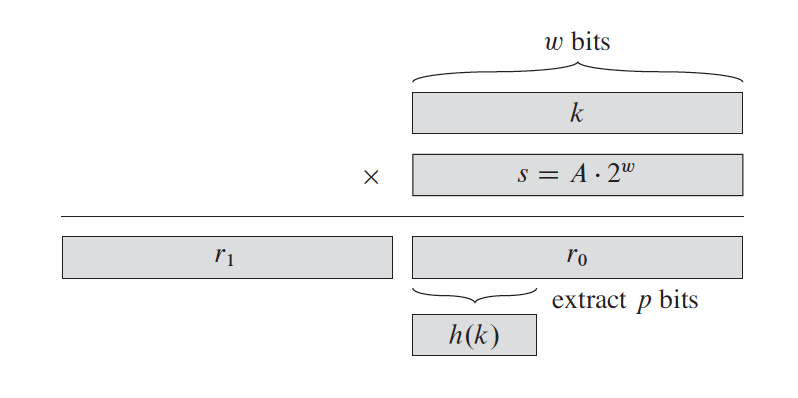
\includegraphics[width=4in]{Cormen_Figure_11_4.png}

%%%%%
\subsubsection{Spring 2018 \#S2}

	% S18 #S2
Given that for an open-address hash table with load factor $\displaystyle \alpha = \frac{n}{m} < 1$, the expected number of probes in unsuccessful search under uniform hashing is at most $\displaystyle \frac{1}{1-\alpha}$, how do you prove the expected number of probes in a successful probe under uniform hashing being at most $\displaystyle \frac{1}{\alpha} \ln \left( \frac{1}{1-\alpha}\right)$?  (Just give a proof sketch, explaining how many probes are needed to locate existing keys.)

\subsubsection{Solution}

This one requires summing probabilities.  I'm going to pass on this one.  

%%%%%
\subsubsection{Fall 2016 \#S9}

	% F16 #S9
Given two hash functions $h_1$ and $h_2$ for Cuckoo hashing under two tables, $T_1$ and $T_2$, 
	\begin{itemize}
		\item Describe the steps involved in inserting a record with the key of $k_{new}$.
		\item Cuckoo hashing can be analyzed by the Cuckoo graph, whose nodes denote table entries and links connect pairs of nodes where given keys can be held.  State when a new key can be inserted successfully based on the Cuckoo graph.
	\end{itemize}

\subsubsection{Solution}

\begin{itemize}
	\item (See above, Spring 2019 \#S2.b)
	\item A new item can be successfully inserted when the Cuckoo graph is acyclic.  
\end{itemize}


%%%%%
\subsubsection{Fall 2015 \#L1}

	% F15 # L1
The utilization efficiency of a hash table depends on its hashing function(s) employed.  Describe with a diagram to illustrate how a multiplication method of hashing works on a machine with word size of $w$ bits for a hash table with $2^p$ entries, $p<w$.  Explain briefly how Cuckoo hashing works under two hash functions of $h_1$ and $h_2$.

\

[Solutions above.]









%\part{Old Exams}
\chapter{Old Exams}
%%%%%%%%%%%%%%%%%%%%%%
\section{Spring 2019}
% Finished copying questions
% Finished indexing

\subsection{Short Questions (Answer all six questions.)}  

\begin{enumerate}
	% S19 S1
	\item Give a big-O (upper bound) estimate for $f(n) = n \log(n!) + 3n^2 + 2n - 10000$, where $n$ is a positive integer.
	\index{Time Complexity!Big-O!S19 \#S1}  

	% S19 S2
	\item The hash table is a widely adopted data structure.  Explain briefly how perfect hashing works.  Separately, what is the situation when a new key cannot be inserted in a Cuckoo hash table separately?
	\index{Hash!Cuckoo Hash!S19 \#S2}
	\index{Hash!Perfect Hashing!S19 \#S2}
	
	% S19 S3
	\item Show your construction of an optimal Huffman code for the set of 10 frequencies:  {\bf a}:2 {\bf b}:6 {\bf c}:5 {\bf d}:8 {\bf e}:13 {\bf f}:34 {\bf g}:34 {\bf h}:15 {\bf i}:27 {\bf j}:9
	
	\index{Huffman Code!Optimal!S19 \#S3}
		
	% S19 S4
	\item Given a weighted directed graph $G = (V,E,w)$ and a shortest path $P$ from $s$ to $t$, if the weight of every edge is doubled to produce $G^* = (V,E,w^*)$, is $P$ still a shortest path in $G^*$?  Explain your reasoning behind your answer. 
	\index{Shortest Path!S19 \#S4}
	
	% S19 S5
	\item BFS (breadth-first search) and DFS (depth-first search):  Give the visited node order for each type of graph search, starting with $S$ below.  
	\index{Breadth First Search!Visited Node Order!S19 \#S5}
	\index{Depth First Search!Visited Node Order!S19 \#S5}
\
	
\hfil	\begin{tikzpicture}[x=20mm, y=10mm]
		\node [circle, draw] (S) at (0,0) {$S$};
		\node [circle, draw] (A) at (2,0) {$A$};
		\node [circle, draw] (B) at (3,-1) {$B$};
		\node [circle, draw] (C) at (2,-2) {$C$};
		\node [circle, draw] (D) at (0,-2) {$D$};
		\draw [-triangle 60] (S) -- (A);
		\draw [-triangle 60] (S) -- (D);
		\draw [-triangle 60] (A) -- (B);
		\draw [-triangle 60] (B) -- (C);
		\draw [-triangle 60] (C) -- (S);
		\draw [-triangle 60] (C) -- (A);
		\draw [-triangle 60] (D) -- (C);
	\end{tikzpicture}
	
	% S19 S6
	\item Many problem have been proved to be NP-complete.  To prove NP-completeness, it is necessary in general to demonstrate two proof components.  What are the two proof components to show a problem being NP-complete?
	
	Being NP-complete, the traveling-salesman problem (TSP) has a 2-approximation solution in polynomial time based on establishing a minimum spanning tree (MST) rooted at the start/end vertex (in polynomial time following MST-PRIM), if the graph edge weights observe the triangle inequality.  Sketch a brief proof to demonstrate that that such a proof satisfies 2-approximation.  

\index{NP!NP-Complete!S19 \#S6}
\index{Traveling Salesman Problem!S19 \#S6}
\index{Minimum Spanning Tree!S19 \#S6}
\index{Two@2-Approximation!S19 \#S6}
	 
\end{enumerate}	

\subsection{Long Questions (Answer all four questions.)}

\begin{enumerate}
	% S19 #L1
	\item Given a B-tree with the minimum degree of $t=3$ below, show the results after (i) deleting $B$, (ii) followed by inserting $M$, (iii) then followed by deleting $T$, and then inserting $M_t$ for $M<M_t<N$
	
\
	
\hfil	\begin{tikzpicture}[x=12mm, y=15mm]
		\node [rectangle, draw, fill=gray] (0) at (0,0) {$P$};
		\node [rectangle, draw, fill=gray] (1) at (-3,-1) {$C G$};
		\node [rectangle, draw, fill=gray] (2) at (3,-1) {$T X$};
		\node [rectangle, draw, fill=gray] (3) at (-5,-2) {$A B$};
		\node [rectangle, draw, fill=white] (4) at (-3,-2) {$D E$};
		\node [rectangle, draw, fill=gray] (5) at (-1,-2) {$JKL NO$};
		\node [rectangle, draw, fill=gray] (6) at (1,-2) {$QRS$};
		\node [rectangle, draw, fill=gray] (7) at (3,-2) {$UV$};
		\node [rectangle, draw, fill=gray] (8) at (5,-2) {$YZ$};
		\draw [-triangle 60] (0) -- (1); 
		\draw [-triangle 60] (0) -- (2); 
		\draw [-triangle 60] (1) -- (3); 
		\draw [-triangle 60] (1) -- (4); 
		\draw [-triangle 60] (1) -- (5); 
		\draw [-triangle 60] (2) -- (6); 
		\draw [-triangle 60] (2) -- (7); 
		\draw [-triangle 60] (2) -- (8); 
	\end{tikzpicture}
	
	\
	
	% S19 #L2
	\item Knapsack problem:  Suppose you want to pack a knapsack with weight limit $W$.  Item $i$ has an integer weight $w_i$ and real value $v_i$.  Your goal is to choose a subset of items with a maximum total value subject to the total weight $\le \ W$.  
	\index{Knapsack Problem!S19 \#L2}

	Let $M[n,W]$ denote the maximum value that a set of items $\in \{1,2,\dots,n\}$ can have such that the weight is no more than $W$.  We have the following recursive formula.  
	
	$$M[n,W] = 
	\begin{cases}
		0 & \text{if $n=0$ or $W=0$} \cr
		M[n-1,W] & \text{if $w_n>W$} \cr
		\max( M[n-1,W-w_n] + v_n, M[n-1,W]) & \text{otherwise} \cr
	\end{cases}
	$$
	
	The time complexity of a simple recursive procedure as given below is exponential.  
\lstset{mathescape}
\begin{lstlisting}
$M(n,W)$
{
	if ($n$==0 or $W$==0) 
		return 0;
	if ($w_n>W$)
		result = $M(n-1,W)$;
	else
		result = $\max\{ v_n + M(n-1,W-w_n), M(n-1,W)\}$;
	return result;
}
\end{lstlisting}

Provide a dynamic programming solution of the Knapsack problem after adding two lines of code to the above procedure.  (Hint:  Use a table to memorize the results.)

	% S19 #L3
	\item Follow the Ford-Fulkerson Algorithm to compute the max flow of the flow network illustrated below.  Show each step to compute the max flow and also show the min cut of the flow network.  
	\index{Max Flow!S19 \#L3}
	\index{Min Cut!S19 \#L3}
	\index{Ford-Fulkerson Algorithm!S19 \#L3}
	
\	
	
\hfil 	\begin{tikzpicture}[x=20mm, y=15mm]
	\node [circle, draw] (S) at (0,0) {$S$};
	\node [circle, draw] (A) at (1,1) {$A$};
	\node [circle, draw] (B) at (3,1) {$B$};
	\node [circle, draw] (C) at (1,-1) {$C$};
	\node [circle, draw] (D) at (3,-1) {$D$};
	\node [circle, draw] (T) at (4,0) {$T$};
	\draw [-triangle 60] (S) -- node [midway, circle, fill=white] {10} (A);
	\draw [-triangle 60] (S) -- node [midway, circle, fill=white] {10} (C);
	\draw [-triangle 60] (A) -- node [midway, circle, fill=white] {12} (B);
	\draw [-triangle 60] (B) -- node [midway, circle, fill=white] {6} (D);
	\draw [-triangle 60] (B) -- node [midway, circle, fill=white] {6} (T);
	\draw [-triangle 60] (C) -- node [midway, circle, fill=white] {5} (A);
	\draw [-triangle 60] (C) -- node [midway, circle, fill=white] {5} (B);
	\draw [-triangle 60] (C) -- node [midway, circle, fill=white] {6} (D);
	\draw [-triangle 60] (D) -- node [midway, circle, fill=white] {14} (T);
\end{tikzpicture}	

	% S19 #L4
	\item The Dijkstra's algorithm (DIJ) solves the single-source shortest-path problem in a weighted directed graph $G=(V,E)$.  Given the graph $G$ below, follow DIJ to find shortest paths from vertex $s$ to all other vertices, with all predecessor edges shaded and estimated distance values from $s$ to all vertices provided at the end of each iteration.  
	
	What is the time complexity of DIJ for a general graph $G=(V,E)$, if the candidate vertices are kept in a binary min-heap?
		
	\index{Dijkstra's Algorithm!S19 \#L4}
	\index{Heaps!Binary Min-Heap!S19 \#L4}
	\index{Time Complexity!S19 \#L4}
	
\

\hfil \begin{tikzpicture}[x=20mm, y=15mm]
	\node [circle, draw] (s) [label=left:{s}] at (0,0) {$0$};
	\node [circle, draw] (t) [label=above:{t}] at (1,1) {$\infty$};
	\node [circle, draw] (x) [label=above:{x}] at (3,1) {$\infty$};
	\node [circle, draw] (y) [label=below:{y}] at (1,-1) {$\infty$};
	\node [circle, draw] (z) [label=below:{z}] at (3,-1) {$\infty$};
	\draw[-triangle 60] (s) to node[circle, fill=white, midway]{10} (t);
	\draw[-triangle 60] (s) to node[circle, fill=white, midway]{5} (y);
	\draw[-triangle 60] (t) to node[circle, fill=white, midway]{1} (x);
	\draw[bend right=20, -triangle 60] (t) to node[circle, fill=white, midway]{2} (y);
	\draw[bend right=20, -triangle 60] (x) to node[circle, fill=white, midway]{4} (z);
	\draw[bend right=20, -triangle 60] (y) to node[circle, fill=white, midway]{3} (t);
	\draw[-triangle 60] (y) to node[circle, fill=white, midway]{9} (x);
	\draw[-triangle 60] (y) to node[circle, fill=white, midway]{2} (z);
	\draw[-triangle 60] (z) to node[circle, fill=white, pos=0.3]{7} (s);
	\draw[bend right=20, -triangle 60] (z) to node[circle, fill=white, midway]{6} (x);
\end{tikzpicture}

\end{enumerate}

%%%%%%%%%%
\subsection{Solutions}

\begin{description}
	\item [Short problem \#1] 
	
	\begin{align*}
		\log(n!) &= \log(n \cdot (n-1) \cdot (n-2) \cdots 2 \cdot 1) \cr
			&= \log(n) + \log(n-1) + \log(n-2) + \cdots + \log(2) + \log 1 \cr
			&\le \log(n) + \log(n) + \log(n) + \cdots + \log(n) + \log (n) \cr
			&= n \log n \cr
		n \log(n!) &\le n \cdot n\log(n) = n^2 \log n \cr
	\end{align*}
	
	Since the $n\log(n!) = O(n^2 \log n)$ is the term of largest asymptotic growth, $f(n) = O(n^2\log n)$.  

	\item [Short problem \#4]  To be the ``shortest path $P$ from $s$ to $t$'' means that it is the path of shortest length, and the length means the sum of the weights of the edges that $P$ traverses.  Consider any path from $v_0$ to $v_k$, $\langle v_0, v_1, v_2,\dots,v_k\rangle$.  The length of this path is $w(v_0) + w(v_1) + \cdots + w(v_k)$.  If all of the edge weights are doubled, the length of each path is doubled, so the path of shortest length under $w$ will still be the shortest under $w^*$
	
	\item [Short problem \#5]  So many answers to this problem.  
	
	BFS:  $S, A, D, C, B$ or $S, D, A, B, C$
	
	DFS:  $S, A, B, C, D$ or $S, D, C, A, B$
	
	\item [Short problem \#6a]
	
	The two proof components to show that a problem $B$ is NP-complete are 
	\begin{enumerate}
		\item An NP-complete decision problem $A$, and 
		\item A polynomial-time transformation that maps instance of $A$ to instances of $B$.  
	\end{enumerate}
	
	The decision problem $B$ is therefore at least as hard as $A$, because if $B$ were easier, one could solve any instance of $A$ by transforming it into an instance of $B$ and using the solution method for $B$.  
	
	\item [Short problem \#6b]  Prove that there is a 2-approximation solution in polynomial time to the Traveling Salesman Problem if the weights satisfy the triangle inequality. 
	 
	Let an actual solution to TSP be the tour $H*$.  

	Let the approximate solution be $H$.  
	
	To make $H$:
	\begin{enumerate}
		\item Grow a minimal spanning tree $T$ with some root $a$, which either Kruskal or Prim can do in polynomial time.  Since it is a minimal spanning tree and has no cycles, its cost cannot be greater than the tour of least cost, so $c(T) \le c(H*)$.  
		\item From the tour, create a walk $W$ starting at, and returning to, $a$.  Since it traverses each edge twice, $c(W) = 2c(T)$.  
		\item Delete from the walk the second appearance of any vertex except $a$ to create the Hamiltonian walk $H$ of a preorder tree walk of $T$.  Because the edge weights satisfy the Triangle Inequality, deleting a vertex does not increase the cost, so $c(H) \le c(W)$.  
		\item Since $c(H) \le c(W) = 2 c(T) \le 2 c(H*)$, the Hamiltonian walk we have created in polynomial time has total cost no more than twice the cost of a perfect solution to the TSP, and thus we have a 2-approximation solution in polynomial time.  
	\end{enumerate}
		
	
\end{description}


%%%%%%%%%%%%%%%%%%%%%
\section{Fall 2018}

\subsection{Short Questions (Answer five of six.)}

\begin{enumerate}
	% F18 #S1
	\item The divide and conquer strategy (D\&C) has been used to solve problem efficiently to reduce the overall computational cost to certain types of problems.
	\begin{enumerate}[label=\alph*.]
		\item Which conditions have to be satisfied for D\&C to solve such problems successfully?  (Clearly state.)
		\item Suppose the size of a problem involved in D\&C is $n=2^k$.  Let the cost in dividing the problems into an equal size is constant and the time to combine solutions to sub-problems is linear.  Write the recurrence relations and then find the tight bound in solving such problems using D\&C.  
	\end{enumerate}
	
	\index{Divide and Conquer!F18 \#S1}
	\index{Recurrence!F18 \#S1}
	\index{Time Complexity!Big-$\Theta$!F18 \#S1}
	
	% F18 #S2
	\item \begin{enumerate}[label=\alph*.]
		\item What is the lower bound for comparisons based sorting algorithm? (Outline the justification of your answer.)
		\item What is the strategy behind greedy algorithm?
	\end{enumerate}
	
	\index{Sorting Algorithms!Comparison Based!F18 \#S2}
	\index{Time Complexity!Big-$\Omega$!F18 \#S2}
	\index{Greedy Algorithms!F18 \#S2}
	
	% F18 #S3
	\item Find the tight bounds (by deriving their upper and lower bounds) of the following expressions.
	\begin{enumerate}[label=\alph*.]
		\item $\displaystyle T(n) = 2 \cdot T \left( \frac{n}{8} \right) + n^{\frac{1}{3}}$
		
		\vskip 6pt
		
		\item $T(n) = log(n!)$
	\end{enumerate}
	
	\index{Time Complexity!Big-$\Theta$!F18 \#S3}
	\index{Recurrence!F18 \#S3}
	
	% F18 #S4
	\item Briefly describe what is dynamic programming.   Can one apply it to solve any optimization problem?  If yes, explain why; if not, what particular conditions must be met.
	
	\index{Dynamic Programming!F18 \#S4}
	
	% F18 #S5
	\item The utilization efficiency of a hash table depends heavily on its hashing function(s) employed.  Describe with a diagram to illustrate how a multiplication method of hashing functions works on a machine with the word size of $w$ bits for a hash table with $2^p$ entries, $p<w$.  
	
	\index{Hash!Utilization Efficiency!F18 \#S5}
	\index{Hash!Multiplication Method!F18 \#S5}
	\index{Hash!Word Size!F18 \#S5}
	
	% F18 #S6
	\item Show your construction of an optimal Huffman code for the set of 7 frequencies:  $\mathbf{a}: 3, \mathbf{b}: 12, \mathbf{c}: 5, \mathbf{d}: 20, \mathbf{e}:16, \mathbf{f}: 34, \mathbf{g}:18$
	
	\index{Huffman Code!Optimal!F18 \#S6}
\end{enumerate}

\subsection{Long Questions (Answer four of five.)}

\begin{enumerate}
	% F18 #L1
	\item Describe how dynamic programming is used to construct an optimal binary search tree.  
	
	Use the following probability of $p$ and $q$, obtain the expected cost of searching an optimal binary search tree constructed by dynamic programming.  
	
	\index{Binary Search Tree!F18 \#L1}
	\index{Dynamic Programming!F18 \#L1}
	
	\
	
\hfil	\begin{tabular}{*9{|r}|}
		\hline
		$i$ & 0 & 1 & 2 & 3 & 4 & 5 & 6 & 7 \cr\hline
		$p_i$ & & 0.04 & 0.06 & 0.08 & 0.06 & 0.10 & 0.12 & 0.10 \cr\hline
		$q_i$ & 0.06 & 0.06 & 0.06 & 0.06 & 0.05 & 0.05 & 0.05 & 0.05 \cr\hline
	\end{tabular}
	
	% F18 #L2
	\item Given the initial B-tree with the minimum node degree of $t=3$ below, show the results 
	
	\begin{enumerate}[label=\alph*.]
		\item After deleting the key of $K$, 
		\item Followed by inserting the key of $L$, 
		\item Then by deleting the key of $J_2$, 
		\item Then by inserting the key of $N_4$ with $N_3 < N_4 < O$, and 
		\item Then by deleting $K_4$.  
	\end{enumerate}
	
	(Show the result after every deletion and after every insertion.)
	
\
	
\hfil	\begin{tikzpicture}[node distance=8 mm and 8 mm]
		\node [rectangle, draw] (a) at (0,0) {$M$};
		\node [rectangle, draw] (b) at (-3,-1) {$J K$};
		\node [rectangle, draw] (c) at (3,-1) {$N O$};
		\node [rectangle, draw, below left=of b] (d) {$A B$};
		\node [rectangle, draw, below=of b] (e) {$J_2 J_3$};
		\node [rectangle, draw, below right=of b] (f) {$K_4 K_6$};
		\node [rectangle, draw, below left=of c] (g) {$M_2 M_4$};
		\node [rectangle, draw, below=of c] (h) {$N_1 N_2 N_3$};
		\node [rectangle, draw, below right=of c] (i) {$O_2 O_3$};
		\foreach \from/\to in {a/b, a/c, b/d, b/e, b/f, c/g, c/h, c/i}
			\draw (\from) -- (\to);
	\end{tikzpicture}
	
	\index{Balanced Search Tree!F18 \#L2}

\

	% F18 #L3
	\item Follow depth-first search (DFS), starting from Node $s$, to traverse the graph shown below, with its edge weights all ignored and the start time equal to 1.  Mark (1) the type of every edge and (2) the discovery and finish times of each node.
	
	Follow breadth-first search (BFS), starting from Node $s$, to traverse the graph shown below, with its edge weights all ignored.  Show the predecessor tree rooted at Node $s$ after BFS, with the number of links (i.e. distance) from Node $s$ to every other node indicated.  
	
	\
	
	\hfil \begin{tikzpicture}[x=15mm, y=15mm]
		\node [circle, draw, label=left:$s$] (s) at (0,0) {};
		\node [circle, draw, label=above:$t$] (t) at (1,1) {};
		\node [circle, draw, label=above:$x$] (x) at (3,1) {};
		\node [circle, draw, label=below:$y$] (y) at (1,-1) {};
		\node [circle, draw, label=below:$z$] (z) at (3,-1) {};
		\foreach \from/\to/\weight in {s/t/10, s/y/-8, t/x/1, y/x/9, y/z/2}
			\draw [-triangle 60] (\from) -- (\to) node [midway, rectangle, fill=white] {\weight};
		\foreach \from/\to/\weight in {z/s/7}
			\draw [-triangle 60] (\from) -- (\to) node [pos=0.3, rectangle, fill=white] {\weight};
		\foreach \from/\to/\weight in {t/y/2, y/t/3, x/z/-4, z/x/6}
			\draw [bend right=20, -triangle 60] (\from) to node [midway, rectangle, fill=white] {\weight} (\to);
			
	\end{tikzpicture}
	
	\index{Depth First Search!F18 \#L3}
	\index{Breadth First Search!F18 \#L3}
	
	%  F18 #L4
	\item The Dijkstra's algorithm (DS) solves the single-source shortest-path problem in a weighted graph $G = (V,E)$ without negative weighted edges or cycles, by edge relaxation at one vertex at a time until all vertices are examined.  Given the graph $G$ below, follow DS to find the shortest paths from vertex $v_1$ to all other vertices, with all predecessor edges shaded and estimated distance values from $v_1$ to all vertices provided at the end.  Also list the sequence of vertices at which relaxation takes place.  
	
	What is the time complexity of DS for a general graph $G = (V,E)$ when candidate vertices are kept in an array?
	
\hfil	\begin{tikzpicture}[node distance = 2cm and 4cm]
		\node [circle, draw, label=above:$v_1$] (v1) {};
		\node [circle, draw, label=above:$v_2$, right=of v1] (v2) {};
		\node [circle, draw, label=above:$v_3$, right=of v2] (v3) {};
		\node [circle, draw, label=below:$v_4$, below= of v1] (v4) {};
		\node [circle, draw, label=below:$v_5$, right=of v4] (v5) {};
		\node [circle, draw, label=below:$v_6$, right=of v5] (v6) {};
		\foreach \from/\to/\label in {v2/v1/1, v3/v2/13, v4/v1/4, v4/v5/3, v5/v2/7, v6/v2/5}{
			\draw [-triangle 60] (\from) -- (\to) node [midway, rectangle, fill=white] {\label};
		}
		\foreach \from/\to/\label in {v1/v5/11, v2/v4/9}{
			\draw [-triangle 60] (\from) -- (\to) node [pos=0.7, rectangle, fill=white] {\label};
		}
		\foreach \from/\to/\label in {v3/v6/6, v6/v3/2}{
			\path [-triangle 60] (\from) edge [bend left] node [midway, rectangle, fill=white] {\label} (\to);
		}
		\foreach \from/\to/\label in {}{
			\draw [triangle 60-triangle 60] (\from) -- (\to) node [midway, rectangle, fill=white] {\label};
		}
 	\end{tikzpicture}
	
	\index{Dijkstra's Algorithm!F18 \#L4}
	\index{Time Complexity!F18 \#L4}

	% F18 #L5
	\item Given the matrix-chain multiplication problem for four matrices sized $30 \times 24$, $24 \times 15$, $15 \times 20$, $20 \times 50$, follow the tabular, bottom-up method in the procedure of \verb|MATRIX-CHAIN-ORDER| below to construct two tables of $m[i,j]$ for all $1\le i, j\le 4$, and $s[i,j]$ for all $1 \le i \le 3$ and $2 \le j \le 4$.  Construct the two tables, with their entry values shown.
	
\begin{lstlisting}[label = MATRIX-CHAIN-ORDER(p), numbers=left, mathescape=True]
$n = p.length - 1$
let $m[1..n, 1.n]$ and $s[1..n-1,2..n]$ be new tables. 
for $i=1$ to $n$
	$m[i][j]= 0$
for $l=2$ to $n$ // $l$ is the chain length.
	for $i=1$ to $n-l+1$
		$j=i+l-1$
		$m[i][j] = \infty$
		for $k=i$ to $j-1$
			$q = m[i,k] + m[k+1,j] + p_{i-1} p_k p_j$
			if $q<m[i,j]$
				$m[i,j] = q$
				$s[i,j] = k$
\end{lstlisting}

	\index{Follow-the-Bouncing-Ball!F18 \#L5}
	
\end{enumerate}

%%%%%%%%%%%%%%%%%%%%
\section{Spring 2018}
% Copying Completed
% Index Completed

\subsection{Short Questions (Answer six of seven.)}

\begin{enumerate}
	% S18 #S1
	\item A problem with size $n$ follows a typical divide-and-conquer approach to have its time complexity of
	$$T(n) = T\left(\frac{n}{4} \right) + T \left( \frac{3n}{4} \right) + c \cdot n$$
	Solve $T(n)$.  (Show your work.)
	
	\index{Time Complexity!S18 \#S1}
	\index{Divide and Conquer!S18 \#S1}
	\index{Recurrence!S18 \#S1}
	
	% S18 #S2
	\item Given that for an open-address hash table with load factor $\displaystyle \alpha = \frac{n}{m} < 1$, the expected number of probes in unsuccessful search under uniform hashing is at most $\displaystyle \frac{1}{1-\alpha}$, how do you prove the expected number of probes in a successful probe under uniform hashing being at most $\displaystyle \frac{1}{\alpha} \ln \left( \frac{1}{1-\alpha}\right)$?  (Just give a proof sketch, explaining how many probes are needed to locate existing keys.)
	\index{Hash!Open Address!S18 \#S2}
	\index{Hash!Load Factor!S18 \#S2}
	\index{Hash!Probes!S18 \#S2}
	\index{Hash!Uniform Hashing!S18 \#S2}

	% S18 #S3
	\item (Lemma 16.2, \S 16.3, page 433) Sketch a proof of the Lemma below, using the tree provided.  
	
	Let $C$ be an alphabet in which each character $c \in C$ has frequency $c.freq$.  Let $x$ and $y$ be two characters in $C$ having the lowest frequencies.  Then there exists an optimal prefix code for $C$ in which the codewords for $x$ and $y$ have the same length and differ only in the last bit. 
	
\hfil	\begin{tikzpicture}[x=15mm, y=10mm]
		\node [circle, draw] (T) {$T$};
		\node [rectangle, draw, below right=of T] (x) {$x$}; 
		\node [circle, draw, below left=of T] (p) { \ };
		\node [circle, draw, below right=of p] (q) { \ };
		\node [rectangle, draw, below left=of 	p] (y) {$y$};
		\node [rectangle, draw, below left=of q] (a) {$a$};
		\node [rectangle, draw, below right=of q] (b) {$b$};
		\foreach \from/\to in {T/x, T/p, p/q, p/y, q/a, q/b}{
			\draw (\from) -- (\to);
		}
	\end{tikzpicture}
	
	\index{Huffman Code!Optimal Prefix Code!S18 \#S3}
	\index{Huffman Code!Codewords!S18 \#S3}

	% S18 #S4
	\item The Dijkstra's algorithm (DS) solves the single-source shortest-path problem in a weighted graph $G = (V,E)$ without negative weighted edges or cycles, by edge relaxation at one vertex at a time until all vertices are examined.  Given the graph $G$ below, follow DS to find the shortest paths from vertex $v_1$ to all other vertices, with all predecessor edges shaded and estimated distance values from $v_1$ to all vertices provided at the end.  Also list the sequence of vertices at which relaxation takes place.  
	
	What is the time complexity of DS for a general graph $G = (V,E)$ when candidate vertices are kept in an array?
	
\hfil	\begin{tikzpicture}[node distance = 2cm and 4cm]
		\node [circle, draw, label=above:$v_1$] (v1) {};
		\node [circle, draw, label=above:$v_2$, right=of v1] (v2) {};
		\node [circle, draw, label=above:$v_3$, right=of v2] (v3) {};
		\node [circle, draw, label=below:$v_4$, below= of v1] (v4) {};
		\node [circle, draw, label=below:$v_5$, right=of v4] (v5) {};
		\node [circle, draw, label=below:$v_6$, right=of v5] (v6) {};
		\foreach \from/\to/\label in {v1/v2/1, v1/v4/4, v2/v3/9, v4/v5/3, v5/v2/7}{
			\draw [-triangle 60] (\from) -- (\to) node [midway, rectangle, fill=white] {\label};
		}
		\foreach \from/\to/\label in {v1/v5/11, v2/v4/5}{
			\draw [-triangle 60] (\from) -- (\to) node [pos=0.7, rectangle, fill=white] {\label};
		}
		\foreach \from/\to/\label in {v3/v6/8, v6/v3/2}{
			\path [-triangle 60] (\from) edge [bend left] node [midway, rectangle, fill=white] {\label} (\to);
		}
		\foreach \from/\to/\label in {v2/v6/5}{
			\draw [triangle 60-triangle 60] (\from) -- (\to) node [midway, rectangle, fill=white] {\label};
		}
 	\end{tikzpicture}
	
	\index{Dijkstra's Algorithm!S18 \#S4}
	\index{Time Complexity!S18 \#S4}
	
	% S18 #S5
	\item \begin{enumerate}[label=\alph*.]
		\item Define height balanced binary tree
		\item Write a pseudo code to determine whether a tree is height balanced?
		\item Obtain a tight bound of your algorithm.
	\end{enumerate}
	
	\index{Binary Search Tree!Height Balanced!S18 \#S5}

\end{enumerate}

\subsection{Long Questions (Answer three of four.)}

\begin{enumerate}

	% S18 #L1
	\item Given the initial B-tree with the minimum node degree of $t=3$ below, show the results 
	
	\begin{enumerate}[label=\alph*.]
		\item After deleting the key of $M_2$, 
		\item Followed by inserting the key of $L$, 
		\item Then by deleting the key of $J_2$, 
		\item Then by inserting the key of $O_1$ with $O < O_1 < O_2$, and 
		\item Then by deleting $K$.  
	\end{enumerate}
	
	(Show the result after every deletion and after every insertion.)
	
\
	
\hfil	\begin{tikzpicture}[node distance=8 mm and 8 mm]
		\node [rectangle, draw] (a) at (0,0) {$M$};
		\node [rectangle, draw] (b) at (-3,-1) {$J K$};
		\node [rectangle, draw] (c) at (3,-1) {$N O$};
		\node [rectangle, draw, below left=of b] (d) {$A B$};
		\node [rectangle, draw, below=of b] (e) {$J_2 J_3$};
		\node [rectangle, draw, below right=of b] (f) {$K_4 K_6$};
		\node [rectangle, draw, below left=of c] (g) {$M_2 M_4$};
		\node [rectangle, draw, below=of c] (h) {$N_1 N_2 N_3$};
		\node [rectangle, draw, below right=of c] (i) {$O_2 O_3$};
		\foreach \from/\to in {a/b, a/c, b/d, b/e, b/f, c/g, c/h, c/i}
			\draw (\from) -- (\to);
	\end{tikzpicture}
	
	\index{Balanced Search Tree!S18 \#L1}

\

	% S18 #L2
	\item A Fibonacci min-heap relies on the procedure of CONSOLIDATE to merge min-heaps in the root list upon the operation of extracting the minimum node.  Given the following Fibonacci min-heap, show every consolidation step and the final heap result after $H.min$ is extracted, with the aid of $A$.  
	
	\index{Heaps!Fibonacci Min Heap!S18 \#L2}
	
\hfil \begin{tikzpicture}[x=13mm, y=13mm]
	\node [circle, draw] (7) at (0,0) {7};
	\node [circle, draw] (24) at (-1,-1) {24};
	\node [circle, draw] (17) at (0,-1) {17};
	\node [circle, draw] (26) at (-2,-2) {26};
	\node [circle, draw] (46) at (-1,-2) {46};
	\node [circle, draw] (30) at (0,-2) {30};
	\node [circle, draw] (35) at (-2,-3) {35};
	\node [circle, draw] (21) at (2,0) {21};
	\node [circle, draw] (18) at (3,0) {18};
	\node [circle, draw] (52) at (4,0) {52};
	\node [circle, draw] (39) at (3,-1) {39};
	\foreach \from/\to in {7/17, 7/24, 7/21, 24/26, 24/46, 17/30, 26/35, 21/18, 18/52, 18/39}
		\draw (\from) -- (\to);
	\node (a) at (-1,1) {$H.min$};
	\draw [-triangle 60] (a) -- (7);
	\node (b) at (2,1) {A};
	\node (c0) at (2.4,1.4) {0};
	\node (c1) at (2.8,1.4) {1};
	\node (c2) at (3.2,1.4) {2};
	\node (c3) at (3.6,1.4) {3};
	\draw (2.2,0.8) rectangle (3.8,1.2);
	\draw (2.6,0.8) -- (2.6,1.2);
	\draw (3.0,0.8) -- (3.0,1.2);
	\draw (3.4,0.8) -- (3.4,1.2);
\end{tikzpicture}	

	% S18 #L3
	\item \begin{enumerate}[label=\alph*.]
		\item To what extent the asymptotic upper bound and lower bound provide insight on running time of an algorithm.
		\item Compare and contrast asymptotic tight bound to the average running time of an algorithm.
		\item Consider the pseudo code of an algorithm given below.  
		\begin{enumerate}
			\item What the value $K$ in line 4 denote?
			\item What the value $m$ in line 8 denote?
			\item When the algorithm terminates, what does the value $m+K$ in line 9 denote?
			\item Find the asymptotic tight bound of Algorithm Test below.
		\end{enumerate}
	\end{enumerate}
	
	\verb|AlgorithmTest(n)|
	
	\begin{lstlisting}[label=Algorithm Test, mathescape=True, numbers=left]
$K=0$
for $i=1$ to $n$
	for $j=1$ to $i$
		$K = K+1$
$m=0$
for $i=1$ to $n-1$
	for $j=i+1$ to $n$
		$m = m+1$
return $(m+K)$
	\end{lstlisting}
	
	\index{Time Complexity!S18 \#L3}
	\index{Time Complexity!Big-$\Theta$!S18 \#L3}
	\index{Follow-the-Bouncing-Ball!S18 \#L3}
	
	% S18 #L4
	
	\item \begin{enumerate}[label=\alph*.]
		\item Define the following classes of a decision problem:  P, NP, and NP-completeness.
		\item Consider the 0-1 knapsack problem with $n$ objects each with its respective pre-defined profit.  The objective is to maximize the total profit that can be accommodated into a container of capacity $W$.  Define appropriate notations for weight and profit of objects, formulate the problem.
		\item Convert of the problem that you have defined in (b) into a decision problem.
		\item Show the problem that you have defined in (c) belongs to NP-class.
		\item Does the problem in (d) belong to the P-class or NP-completeness. (Justify your answer.)
		\item If principle of optimality be applicable to solve the problem defined in (c), formulate it.  Otherwise, explain why not.  
		\item What would be your explanation, if 0-1 knapsack problem is solved by dynamic programming in polynomial time?
	\end{enumerate}
	
	\index{NP!NP-Complete!S18 \#L4}
	\index{Knapsack Problem!S18 \#L4}
	\index{Decision Problem!S18 \#L4}
	\index{Principle of Optimality!S18 \#L4}
	\index{Dynamic Programming!S18 \#L4}
	
\end{enumerate}



%%%%%%%%%%%%%%%%%%%%%
\section{Spring 2017}

\subsection{Short Questions (Answer all six.)}

\begin{enumerate}
	% S17 #S1
	\item \begin{enumerate}[label=\alph*.]
		\item Define height balanced binary tree.
		\item Write a pseudo code to determine whether a tree is height balanced?
		\item Obtain the tight bound of your algorithm.
	\end{enumerate}
	
	\index{Binary Search Tree!Height Balanced!S17 \#S1}
	\index{Time Complexity!Big-$\Theta$!S17 \#S1}
	
	% S17 #S2
	\item Suppose you have keys of $N$ objects stored in an array in the ascending order of key values.  Also assume that there is duplicate entry in the key.  
	\begin{enumerate}[label=\alph*.]
		\item Describe an efficient algorithm with the pseudo code that helps you to search for the object given the key. (The algorithm must return null value if the key is not in the array.) 
		\item Obtain the tight upper bound for your algorithm.
	\end{enumerate}
	
	\index{Key Array!S17 \#S2}
	\index{Key Array!Duplicate Entry!S17 \#S2}
	\index{Key Array!Search Algorithm!S17 \#S2}
	\index{Time Complexity!Big-O!S17 \#S2}

	% S17 #S3
	\item	\begin{enumerate}[label=\alph*.]
		\item Define strongly connected components as applied to directed graphs.
		\item Some potential application of strongly connected components.
		\item Provide a pseudo code for obtaining strongly components of a directed graph.  (Hint:  Use depth first search on appropriately transformed graphs.)
	\end{enumerate}
	
	\index{Strongly Connected Components!S17 \#S3}
	\index{Strongly Connected Components!Applications!S17 \#S3}
	\index{Strongly Connected Components!Code for Obtaining!S17 \#S3}
	
	% S17 #S4
	\item Find the tight for the recurrence relation below without using the master theorem (show all the steps):
	$$T(n) = T(n/2) + n$$
	
	\index{Recurrence!S17 \#S4}
	\index{Time Complexity!Big-$\Theta$!S17 \#S4}
	
	% S17 #S5
	\item	\begin{enumerate}[label=\alph*.]
		\item What are the properties of min heap and max heaps.
		\item What is the preferred data structure of implementing binary heap, also justify your answer.
		\item What is the time complexity of merging two different min heaps each of size $n$ and $m$.
	\end{enumerate}
	
	\index{Heaps!Preferred Data Structure!S17 \#S5}
	\index{Heaps!Properties!S17 \#S5}
	\index{Heaps!Merging!S17 \#S5}

	% S17 #S6
	\item Briefly describe the minimum spanning tree.  Sketch an algorithm to obtain a minimum spanning tree.
	
	\index{Minimum Spanning Tree!S17 \#S6}

	\begin{enumerate}[label=\alph*.]
		\item
	\end{enumerate}

\end{enumerate}

\subsection{Long Questions (Answer three of four.)}

\begin{enumerate}
	% S17 #L1
	\item (Problem is related to dynamic programming formulation and optimal sub structure)
	\begin{enumerate}[label=\alph*.]
		\item Explain what do you understand by ``principle of optimality.''
		\item Consider the problem of finding the longest common subsequences (LCS) in a pair of sequences, namely $X(x_1, x_2,\dots, x_m)$ and $Y(y_1, y_2, \dots, y_n)$
		\begin{enumerate}
			\item A brute force approach is to generate all possible subsequences of $X$ and see whether it is also a subsequence of $Y$.  What is the number of possible subsequence of $X$?
			\item Obtain the optimal substructure of an LCS.  
		\end{enumerate}
		
		\item Consider a chain matrix multiplication problem, $m_1 \times m_2 \times \cdots \times m_n$.  It associative, but not commutative.  
		\begin{enumerate}
			\item  A brute force approach is to generate all possible ways of parenthsizing the matrix chain and compute the total number of operations.  What is the number of possible grouping of the matrix chain?
			\item Obtain the structure of the optimal parenthesization and then the recursive definition of the minimal cost of parenthesizing the product $m_i, m_{i+1}, m_j$.  
		\end{enumerate}
		
	\end{enumerate}
	
	\index{Dynamic Programming!Principle of Optimality!S17 \#L1}
	\index{Dynamic Programming!Longest Common Subsequence!S17 \#L1}
	\index{Dynamic Programming!Optimal Substructure!S17 \#L1}
	\index{Dynamic Programming!Chain Matrix Multiplication!S17 \#L1}
	\index{Dynamic Programming!Combinations!S17 \#L1}

	% S17 #L2
	% Similar to S15 #L3
	\item	(Similar to S15 \#L3)
	\begin{enumerate}[label=\alph*.]
		\item Compare and contrast P, NP, NP-complete, and NP-hard.
		\item Based on current conjecture, draw a Venn diagram to show the relationship among these classes of problem.
		\item Suppose there $n$ clauses and $m$ propositions in a given 3p-sat problem.  How many possible interpretations are there?  What is the time complexity of testing the satisfiability of a given interpretation?  What is the time and space complexity of testing the satisfiability of the clauses?
		\item 3-p sat problem is NP-complete, but people still have published papers by applying heuristics strategy and showing that they were able to solve it with large number of distinct propositions (say 100) and large number of clauses (say 200).  To avoid any bias, they have generated the clauses and the set of propositions randomly.  How would you start investigating their results?  Can their results be generalized?
		\item Suppose a single NP-complete problem is solved in polynomial algorithm, what can you state about the entire NP-complete class as well as the NP-hard class.
		
	\end{enumerate}

	\index{NP!Relationship of P, NP, NP-complete, and NP-hard!S17 \#L2}
	\index{NP!3-p sat!S17 \#L2}
	\index{NP!Heuristics!S17 \#L2}
	\index{NP!Randomly Generated Propositions and Clauses!S17 \#L2}
	
	% S17 #L3
	\item (Same instructions, different graph, as S15 \#S7)
	The Edmonds-Karp Algorithm (EK) follows the basic Ford-Fulkerson method with breadth-first search to choose the shortest augmenting path (in terms of the number of edges involved) for computing the maximum flow iteratively from vertex $s$ to vertex $t$ in a weighted directed graph.  Illustrate the maximum flow computation process (including the augmenting path chosen for each iteration and its resulting residual network) via EK for the graph depicted below.  
	
\hfil\begin{tikzpicture}[x=15mm, y=15mm]
	\node [circle, draw] (s) at (0,0) {$s$};
	\node [circle, draw] (v1) at (2,1) {$v_1$};
	\node [circle, draw] (v2) at (3,-1) {$v_2$};
	\node [circle, draw] (v3) at (4,1) {$v_3$};
	\node [circle, draw] (t) at (6,0) {$t$};
	\foreach \from/\to/\weight in {s/v1/16, s/v2/13, v1/v2/4, v1/v3/12, v3/v2/9, v3/t/20}
		\draw [-triangle 60] (\from) -- (\to) node [midway, circle, fill=white] {\weight};
	\path [-triangle 60] (v2) edge [bend left=10] node [midway, rectangle, fill=white] {17} (t);
	\path [triangle 60-triangle 60] (t) edge [bend left=10] node [midway, rectangle, fill=white] {8} (v2);
\end{tikzpicture}

	SHOULD THE EDGE WITH WEIGHT 8 BE BIDIRECTIONAL?

	\index{Max Flow!Augmenting Path!S17 \#L3}	
	
	% S17 #L4
	\item  (Same as Fall 2016 \#L4 and S15 \#L4)
	
	 Given a set of 4 keys, with the following probabilities, determine the cost and the structure of an optimal BST (binary search tree), following the tabular, bottom-up method realized in the procedure of \verb|OPTIMAL-BST| below to construct and fill $e[1..5, 0..4], w[1..5,0..4]$ and $root[1..4,1..4]$.
	
\hfil	\begin{tabular}{>{$}r<{$}|ccccc}
		i & 0 & 1 & 2 & 3 & 4 \cr\hline
		p_i & & 0.10 & 0.08 & 0.22 & 0.21 \cr
		q_i & 0.06 & 0.12 & 0.07 & 0.05 & 0.09 \cr
	\end{tabular}
	
\

Construct and fill the three tables, and show the optimal BST obtained.  

\

\verb|OPTIMAL-BST(p,q,n)|

\begin{lstlisting}[mathescape=true, numbers=left]
let $e[1..n+1, 0..n]$, $w[1..n+1, 0..n]$, and $root[1..n, 1..n]$ be new tables.
for $i=1$ to $n+1$
	$e[i, i-1] = q_{i-1}$
	$w[i, i-1] = q_{i-1}$
for $l=1$ to $n$
	for $i=1$ to $n-l+1$
		$j = i+l-1$
		$e[i,j] = \infty$
		$w[i,j] = w[i,j-1] + p_j + q_j$
		for $r=i$ to $j$
			$t = e[i,r-1] + e[r+1,j] + w[i,j]$
			if $t < e[i,j]$
				$e[i,j] = t$
				$root[i,j] = r$
return $e$ and $root$
\end{lstlisting}

	\index{Binary Search Tree!Optimal!S17 \#L4}	


\end{enumerate}



%%%%%%%%%%%%%%%%%%%
\section{Fall 2016}
% Finished copying questions
% Finished indexing

\subsection{Short Questions.  (Answer eight of ten.)}

\begin{enumerate}
	% F16 #S1
	\item \begin{enumerate}
		\item Define an upper and the tight time bound of an algorithm.
		\item In which way the average time bound will add more value to the tight bound?
	\end{enumerate}
	
	\index{Time Complexity!Big-O!F16 \#S1}
	\index{Time Complexity!Big-$\Theta$!F16 \#S1}

	% F16 #S2	
	\item\begin{enumerate}
		\item Briefly describe a quick sort algorithm for sorting objects in an ascending order of their keys.
		\item What is the best and worst case time complexity of quick sort and the reason for such complexity?
	\end{enumerate}
	
	\index{Quick Sort Algorithm!F16 \#S2}
	\index{Time Complexity!F16 \#S2}
	
	% F16 #S3
	\item Find the tight [time bound, time complexity?] for the recurrence relations without using the master theorem. 
	\begin{enumerate}
		\item $T(n) = T(n-2) + 2 \lg(n)$
		\item $T(n) = T(\sqrt{n}) + \lg(n)$
	\end{enumerate}
	
	\index{Time Complexity!Big-$\Theta$!F16 \#S3}
	\index{Recurrence!F16 \#S3}
	\index{Master Theorem!F16 \#S3}
	
	% F16 #S4
	\item \begin{enumerate}
		\item What are the properties of min heap and max heaps.
		\item What is the preferred data structure of implementing binary heap, also justify your answer.
		\item What is the time complexity of merging two different min heap with sizes of $n$ and $m$.
	\end{enumerate}
	
	\index{Heaps!Min Heap!F16 \#S4}
	\index{Heaps!Max Heap!F16 \#S4}
	\index{Heaps!Binary Heap!F16 \#S4}
	\index{Heaps!Min Heap!Merging!F16 \#S4}
	
	% F16 #S5
	\item Suppose there are $n$ clauses and $m$ variables (propositions) in a given $3-p$ sat problem.
	\begin{itemize}
		\item How many possible interpretations are there?
		\item Find the tight bound of checking for satisfiability of the $n$ clauses.  
	\end{itemize}
	
	\index{NP!3-p sat!F16 \#S5}
	\index{Time Complexity!Big-$\Theta$!F16 \#S5}
	
	% F16 #S6
	\item \begin{enumerate}
		\item Briefly define greedy strategy.
		\item Will it always yield an optimal solution?  If not, provide an algorithm that yields an optimal solution.  
	\end{enumerate}
	
	\index{Greedy Algorithms!F16 \#S6}
	
	% F16 #S7
	\item \begin{enumerate}
		\item Define strongly connected components.
		\item Does a strongly connected component graph cyclic or acyclic?  Justify your answer.  
	\end{enumerate}
	
	\index{Strongly Connected Components!F16 \#S7}
	
	% F16 #S8
	\item Mark true/false (T/F) against the following statements.  
	
	\begin{itemize}
		\item A binary search tree of size $N$ will always find a key at most $O(\lg N)$ time
		\item A breadth first search can be considered as a special case of heuristic search algorithm.
		\item An optimal binary search tree is not necessarily being a balanced tree.
		\item A dynamic programming approach uses top-down problem solving strategy to solve optimization problem.
	\end{itemize}
	
	\index{Breadth First Search!F16 \#S8}
	\index{Binary Search Tree!Optimal!F16 \#S8}
	\index{Dynamic Programming!F16 \#S8}
	\index{Top-Down!F16 \#S8}
	
	% F16 #S9
	\item Given two hash functions $h_1$ and $h_2$ for Cuckoo hashing under two tables, $T_1$ and $T_2$, 
	\begin{itemize}
		\item Describe the steps involved in inserting a record with the key of $K_{new}$.
		\item Cuckoo hashing can be analyzed by the Cuckoo graph, whose nodes denote table entries and links connect pairs of nodes where given keys can be held.  State when a new key can be inserted successfully based on the Cuckoo graph.
	\end{itemize}
	
	\index{Hash!F16 \#S9}
	\index{Hash!Cuckoo Hash!F16 \#S9}
	
	% F16 #S10
	\item The recurrence of Procedure CUT-ROD$(p,n)$ is given by 
	$$T(n) = 1 + \sum_{j=1}^{n-1} T(j), \ T(0) = 1$$
	Solve $T(n)$.  
	
	\index{Recurrence!F16 \#10}
	\index{Follow-the-Bouncing-Ball!F16 \#S10}
	
\end{enumerate}

\subsection{Notes}

	\#5.  According to Long Problem \#1, ``3-p sat'' means ``three-proposition satisfiability.'' There is a field of Boolean satisfiability problems called 3-sat.  It's an NP-complete problem.  
	
	\#7.  Strongly connected components in Cormen \S 22.5
	
	\#8.  ``Heuristic'' not in Cormen.
	
	\#9.  ``Cuckoo hashing'' not in Cormen.
	
	\#10.  $T(n) = 2^n$.  
	
\subsection{Long Questions.  (Answer three of four.)}

\begin{enumerate}
	% F16 #L1
	\item \begin{enumerate}
		\item Briefly describe NP-class, P-class, NP-complete, and NP-hard.
		\item Show the conjectured relationship among the classes NP-class, P-class, NP-complete, and NP-hard.
		\item Show that counting $n$ objects with integer key values belongs to NP-class.  
		\item Provide the steps involved in showing whether a problem belongs to NP-complete or not.
		\item Illustrate the steps in step d by showing 3 proposition satisfiability (3-p sat) problem belongs to NP-complete.
		\item Provide a pseudo code that attempt to solve 3-p sat problem heuristically.
	\end{enumerate}
	
	\index{NP!F16 \#L1}
	\index{NP!3-p sat!F16 \#L1}

	% F16 #L2
	\item 	\begin{enumerate}
		\item 	Explain what do you understand by ``principle of optimality'' in the context of dynamic programming.
		\item Characterize 0-1 knapsack problem in terms of objective function, constraints, and the time and space complexity.  (Assume there are $n$ objects.  Suppose an object $i$ has weight $w_i$ and profit $p_i$.  The overall capacity of the container is $W$).
		\item Show the 0-1 knapsack problem belong to NP-class.
		\item Does it belong to P-class?  (Provide an explanation accordingly.)
		\item Write down the basic rule that satisfy the principle of optimality and domain related constraints to the following problems:
		\begin{enumerate}
			\item 0-1 knapsack problem
			\item Pairwise shortest path problem
		\end{enumerate}
	\end{enumerate}
	
	\index{Dynamic Programming!Principle of Optimality!F16 \#L2}
	\index{Knapsack Problem!F16 \#L2}
	
	% F16 #L3
	\item Given an initial B-tree with the minimum node degree of $t=2$ below, show the results 
	\begin{enumerate}
		\item after inserting the key of $H$, and 
		\item then followed by deleting two keys in order:  $X$ then $P$.  (show the result after insertion and the result after each deletion.)
	\end{enumerate}
	
	\index{Balanced Search Tree!F16 \#L3}
	
\
	
\hfil	\begin{tikzpicture}[x=12mm, y=15mm]
		\node [rectangle, draw] (0) at (0,0) {$P$};
		\node [rectangle, draw] (1) at (-4,-1) {$C G M$};
		\node [rectangle, draw] (2) at (3,-1) {$T X$};
		\node [rectangle, draw] (3) at (-7,-2) {$A B$};
		\node [rectangle, draw] (4) at (-5,-2) {$D E F$};
		\node [rectangle, draw] (5) at (-3,-2) {$J K L$};
		\node [rectangle, draw] (6) at (-1,-2) {$N O$};
		\node [rectangle, draw] (7) at (1,-2) {$Q R S$};
		\node [rectangle, draw] (8) at (3,-2) {$U V$};
		\node [rectangle, draw] (9) at (5,-2) {$Y Z$};
		\draw [-triangle 60] (0) -- (1); 
		\draw [-triangle 60] (0) -- (2); 
		\draw [-triangle 60] (1) -- (3); 
		\draw [-triangle 60] (1) -- (4); 
		\draw [-triangle 60] (1) -- (5); 
		\draw [-triangle 60] (1) -- (6); 
		\draw [-triangle 60] (2) -- (7); 
		\draw [-triangle 60] (2) -- (8); 
		\draw [-triangle 60] (2) -- (9); 
	\end{tikzpicture}

	% F16 #L4
	\item (Same as S15 \#L4 and S17 \#L4)  
	Given a set of 4 keys, with the following probabilities, determine the cost and the structure of an optimal binary search tree, following the tabular, bottom-up method realized in the procedure of \verb|OPTIMAL-BST| below to construct and fill tables $e[1..5, 0..4]$, $w[1..5, 0..4]$, and $root[1..4, 1..4]$.  
	
	\index{Binary Search Tree!Optimal!F16 \#L4}
	
	\hfil \begin{tabular}{c|ccccc}
		$i$ & 0 & 1 & 2 & 3 & 4 \cr\hline
		$p_i$ & & & & \cr
		$q_i$ & & & & \cr
	\end{tabular}
	
	\begin{lstlisting}[mathescape=true]
let $e[1..n + 1, 0..n ]$, $w[1..n+1, 0..n]$, and $root[1..n, 1..n]$ be new tables.
for $i=1$ to $n+1$
	$e[i, i-1] = q_{i-1}$
	$w[i, i-1] = q_{i-1}$
for $l=1$ to $n$
	for $i=1$ to $n-l+1$
		$j = i+l-1$
		$e[i,j] = \infty$
		$w[i,j] = w[,i,j-1] + p_j + q_j$
		for $r=i$ to $j$
			$t = e[i, r-1] + e[r+1,j] + w[i,j]$
			if $i<e[i,j]$
				$e[i,j] = t$
				$root[i,j] = r$
return $e$ and $root$
	\end{lstlisting}

\end{enumerate}

\subsection{Notes}

\#4 is the same as Cormen 15.5-2

	\begin{enumerate}
		\item 
	\end{enumerate}
	


%%%%%%%%%%%%%%%%%%%%
\section{Fall 2015}

\subsection{Short Questions (Answer all eight.)}

\begin{enumerate}
	% #F15 S1
	\item Show that for arbitrary real constants $a$ and $b$ with $b>0$, we have $(n+a)^b = \Theta(n^b)$.
	\index{Time Complexity!Big-$\Theta$!F15 \#S1}
	
	% #F15 S2
	\item Use the recursion-tree technique to derive the tight lower and upper bounds of the recursion $T(n) = T(n/3) + T(2n/3) + cn$.
	\index{Recursion!F15 \#S2}
	\index{Time Complexity!Big-$\Theta$!F15 \#S2}

	% #F15 S3
	\item What is the time complexity of insertion sort algorithm?  Suppose you already know the total number of keys and range of the key values.  What would be the best and worst results you will get when sorting $n$ items?  In addition to the previous information, if you already know that the key values are uniformly distributed, what would be your best and worst results?  (Make sure you sketch the algorithm and provide rationale of your expected results.  Do NOT derive the result.)
	\index{Insertion Sort!F15 \#S3}

	% #F15 S4
	\item Define minimum spanning tree.  What are the salient features of a minimum spanning tree?  Name a couple of [two] algorithms that will help to find the minimum spanning tree from a graph.  Out of the two, which one would you prefer and specify why.  
	\index{Minimum Spanning Tree!F15 \#S4}
	
	% #F15 S5
	\item Mark True or False for each of the following statements.  
	\begin{enumerate}[label=\alph*.]
		\item Greedy strategy sometimes finds the best or the optimal solution.
		\item Dynamic programming will always find the optimal solution even when the principal of optimality condition is not satisfied.
		\item (Same as S5 \#S9b) Breadth first search is a special case of heuristic search algorithm.
		\item Some problems that belong to NP-class can be solved polynomially.  
		\item Satisfiability problem of propositional calculus is NP-complete.
	\end{enumerate}
	\index{Greedy Algorithms!F15 \#S5}
	\index{Dynamic Programming!Principle of Optimality!F15 \#S5}
	\index{Breadth First Search!F15 \#S5}
	\index{Heuristic!F15 \#S5}
	\index{NP!F15 \#S5}
	\index{NP!NP-Complete!F15 \#S5}
	\index{NP!Propositional Calculus!F15 \#S5}
		
	% #F15 S6
	\item Obtain the optimal parenthesize for a chain multiplication given the $S$ matrix as has been explained in the textbook or in class.  (Show the working details.)
	
	\
	
\hfil	\begin{tabular}{cc|ccccccc}
	
		\multicolumn{7}{c}{[some letter] $\to$} \cr
		&& 1 & 2 & 3 & 4 & 5 & 6 \cr\hline
		&7 & 4 & 4 & 4 & 3 & 5 & 6 \cr
	\multirow{ 2}{*}{$d \uparrow$} &6 & 4 & 4 & 4 & 3 & 5 \cr
		&5 & 3 & 3 & 4 & 4 \cr
		&4 & 1 & 2 & 3 \cr
		&3 & 1 & 2 \cr
		&2 & 1 \cr
	\end{tabular}
	\index{Dynamic Programming!Chain Matrix Multiplication!F15 \#S6}

	% F15 #S7
	\item Mark True or False against the following statements.
	\begin{enumerate}[label=\alph*.]
		\item  (Same as S15 \#9a) A binary search tree of size $N$ will always find a key in at most $O(\log N)$ time.
		\item An optimal binary search is not necessary a balanced tree.
		\item A binary heap always maintains a balanced tree as practical as it can be.
		\item To implement a priority queue binomial heap is preferred over binary heap.
		\item A graph formed by strongly connected components, a strongly connected components graph (SCC) is always a minimum spanning tree.  
	\end{enumerate}
	\index{Binary Search Tree!Optimal!F15 \#S7}
	\index{Heaps!Binary Min-Heap!F15 \#S7}
	\index{Heaps!Binary Min-Heap!Priority Queue!F15 \#S7}
	\index{Priority Queue!F15 \#S7}
	\index{Strongly Connected Components!F15 \#S7}
	
	% F15 #S8
	\item For any $n$-key B-tree of height $h$ and with minimum node degree of $t \ge 2$, prove that $h$ is no larger than $\log_t \frac{n+1}{2}$.  (Hint:  Consider the number of keys stored in each tree level.)
	\index{Balanced Search Tree!F15 \#S8}
\end{enumerate}
	
\subsection{Long Questions (Answer three of four.)}

\begin{enumerate}
	% F15 # L1
	\item The utilization efficiency of a hash table depends on its hashing function(s) employed.  Describe with a diagram to illustrate how a multiplication method of hashing works on a machine with word size of $w$ bits for a hash table with $2^p$ entries, $p<w$.  Explain briefly how Cuckoo hashing works under two hash functions of $h_1$ and $h_2$.
	\index{Hash!Cuckoo Hash!F15 \#L1}
	\index{Hash!Multiplication Method!F15 \#L1}
	
	% F15 # L2
	\item Given the initial B-tree with the minimum node degree of $t-3$ below, show the results (a) after inserting two keys in order:  $Q$ then $W$, and (b) followed by deleting two keys in order:  $Y$ then $T$.  (Show the aggregate result after insertion and another result after deletion.)
	
	\
	
\hfil	\begin{tikzpicture}[x=15mm, y=15mm]
		\node [rectangle, draw] (GMPX) at (0,0) {$G \ M \ P \ X$};
		\node [rectangle, draw] (ACDE) at (-4,-1) {$A \ C \ D \ E$};
		\node [rectangle, draw] (JK) at (-2,-1) {$J \ K$};
		\node [rectangle, draw] (NO) at (0,-1) {$N \ O$};
		\node [rectangle, draw] (RSTUV) at (2,-1) {$R \ S \ T \ U \ V$};
		\node [rectangle, draw] (YZ) at (4,-1) {$Y \ Z$};
		\foreach \from/\to in {GMPX/ACDE, GMPX/JK, GMPX/NO, GMPX/RSTUV, GMPX/YZ}
			\draw [-triangle 60] (\from) -- (\to);
	\end{tikzpicture}
	\index{Balanced Search Tree!F15 \#L2}
	
	% F15 # L3
	\item In the following pseudo code, 
	\begin{enumerate}[label=\alph*.]
		\item Write the formula to determine the number of add operations at line 5 when the algorithm terminates.  
		\item What is the space complexity?
		\item Find the following time bounds of this algorithm:  Upper, lower, and tight. (Must show all the details of your work.)
	\end{enumerate}
	
	\
	
	\verb|Algorithm Count|
	
	\begin{lstlisting}[numbers=left, mathescape=true]
$Cnt = 0$
for $i=1$ to $n$ do {
	for $j = 1$ to $i^2$ do {
		for $k=1$ to $j$ do {
			$Cnt = Cnt + 1$
		}
	}
}
	\end{lstlisting}
	
	Note that I have corrected line 3 from \ \verb|for j=i^2 to i do{|
	
	\index{Space Complexity!F15 \#L3}
	\index{Time Complexity!F15 \#L3}
	\index{Follow-the-Bouncing-Ball!F15 \#L3} 
	
	% F15 #L4
	\item\begin{enumerate}[label=\alph*.]
		\item Describe maximum clique problem.
		\item Write a pseudo code to obtain the maximum clique of a graph with $N$ nodes and $E$ edges using generate and test strategy.  That is, generate all possible subsets of vertices and test whether the subset is a clique.  (Make any assumptions explicitly.)
		\item Find the time and space complexity of your algorithm.
		\item Describe the 0-1 knapsack problem.
		\item Show that the 0-1 knapsack problem belongs to NP-class.
		\item Briefly describe a practical way of solving a 0-1 knapsack problem and its time complexity assuming that the knapsack capacity is $K$ and there are $M$ objects.  The weight and profit of an object $i$ are denoted by $w_i$ and $p_i$ respectively.  
	\end{enumerate}
	
	\index{Maximum Clique!F15 \#L4}
	\index{Knapsack Problem!F15 \#L4}
	
\end{enumerate}


%%%%%%%%%%%%%%%%%%%
\section{Spring 2015}

\subsection{Short Questions}

Answer all of the questions.  All short questions, but Q3, carry 2 points each.  Question 3 will be evaluated for 4 points.

\begin{enumerate}
	% S15 #S1
	\item Briefly define upper, lower, and tight time bound of an algorithm.  How does an average time complexity related to any of these bounds?
	\index{Time Complexity!S15 \#S1}
	
	% S15 \#S2
	\item In terms of run time efficiency, compare and contrast quick sort and merge sort.  What is the best and the worst case time complexity of the quick sort algorithm?  Also state under what conditions one may expect these two extreme cases.
	\index{Quick Sort!S15 \#S2}
	\index{Merge Sort!S15 \#S2}
	\index{Time Complexity!S15 \#S2}
	
	% S15 #S3
	\item Find the tight bounds of the following sums.  
	\begin{enumerate}
		\item $\displaystyle \sum_{i=1}^n i^3 a^i$ where $a$ is a constant greater than 1
		\item $\displaystyle \sum_{i=1}^n \log (i^3)$ 
	\end{enumerate}
	\index{Time Complexity!Big-$\Theta$!S15 \#S3}
	
	% S15 \#S4
	\item Mark true/false (T/F) against the following statements:
	\begin{enumerate}
		\item Connecting any pair of nodes in a minimum spanning tree will always form a cycle.
		\item Building strongly connected component graph of a directed graph of $N$ nodes takes $O(N^2)$ time.  
		\item A graph formed by strongly connected component nodes, a strongly connected component graph (SCC) is always a minimum spanning tree.
		\item SCC graph will be useful in determining articulation node in a graph.
	\end{enumerate}
	\index{Minimum Spanning Tree!S15 \#S4}
	\index{Strongly Connected Components!Building the Graph!S15 \#S4}
	\index{Minimum Spanning Tree!S15 \#S4}
	\index{Articulation Node!S15 \#S4}
	
	% S15 #S5
	\item Use a binary tree representation to illustrate every operation of \verb|MIN HEAPSORT| involved when sorting array $A = \{5,13,2,25,7\}$ without auxiliary storage.
	\index{Heaps!{\tt MIN HEAPSORT}!S15 \#S5}
	
	% S15 #S6
	\item Show your construction of an optimal Huffman code for the set of 7 frequencies:  $\mathbf{a}:2 \ \  \mathbf{b}:3 \ \ \mathbf{c}:5 \ \ \mathbf{d}:8 \ \ \mathbf{e}:13 \ \ \mathbf{f}:21 \ \ \mathbf{g}:34$
	\index{Huffman Code!Optimal!S15 \#S6}

	% S15 #S7	
	% S17 #L3
	\item (Same instructions, different graph, as S17 \#L3)
	The Edmonds-Karp Algorithm (EK) follows the basic Ford-Fulkerson method with breadth-first search to choose the shortest augmenting path (in terms of the number of edges involved) for computing the maximum flow iteratively from vertex $s$ to vertex $t$ in a weighted directed graph.  Illustrate the maximum flow computation process (including the augmenting path chosen for each iteration and its resulting residual network) via EK for the graph depicted below.  
	
\
	
\hfil\begin{tikzpicture}[x=15mm, y=15mm]
	\node [circle, draw] (s) at (0,0) {$s$};
	\node [circle, draw] (v1) at (2,1) {$v_1$};
	\node [circle, draw] (v2) at (2,-1) {$v_2$};
	\node [circle, draw] (v3) at (4,1) {$v_3$};
	\node [circle, draw] (v4) at (4,-1) {$v_4$};
	\node [circle, draw] (t) at (6,0) {$t$};
	\foreach \from/\to/\weight in {s/v1/16, s/v2/13, v1/v3/12, v2/v1/4, v2/v4/14, v3/v2/9, v3/t/20, v4/v3/7, v4/t/4}
		\draw [-triangle 60] (\from) -- (\to) node [midway, circle, fill=white] {\weight}; 
\end{tikzpicture}
		\index{Max Flow!Augmenting Path!S15 \#S7}	

	% S15 \#S8
	\item Briefly describe priority queue that maintains the highest key value.  What is the preferred data structure for implementing priority queue?  If the following keys with values 33, 22, 35, 40, 36, and 41 were added in the given order to an empty priority queue that maintains highest key value at the root, draw the priority queue at the end of all the given set of keys.  (Show all the key values and their indices.)
	\index{Priority Queue!S15 \#S8}
	
	% S15 \#S9
	\item Mark true/false against the following statements. 
	\begin{enumerate}
		\item (Same as F15 \#S7a) A binary search tree of size $N$ will always find a key in at most $O(\log N)$ time.
		\item (Same as F15 \#S5c) A breadth first search algorithm can be considered as a special case of heuristic search algorithm.
		\item An optimal binary search tree is not necessarily a balanced tree.
		\item A dynamic programming approach uses top-down problem solving strategy to solve optimization problem.
	\end{enumerate}
	\index{Binary Search Tree!S15 \#S9}
	\index{Breadth First Search!S15 \#S9}
	\index{Heuristic !S15 \#S9}
	\index{Binary Search Tree!Optimal!S15 \#S9}
	\index{Balanced Search Tree!S15 \#S9}
	\index{Dynamic Programming!S15 \#S9}

\end{enumerate}

\subsection{Long Questions (Answer three of four.)}

\begin{enumerate}
	% S15 #L1
	\item \begin{enumerate}
		\item Suppose you have to find a solution to a problem that belongs to NP-complete class.  Clearly summarize the steps that will help you to find the solution of the problem.  
		\item John, an undergraduate student, recently took data structure course, states that heuristics algorithms always solve NP-complete problems.  He cites simplex methods as an example.  If you agree with John, justify why or why not.  
		\item What is the strategy behind a greedy algorithm?  Will it always provide an optimal solution?  If yes explain why, otherwise say why not.  
		\item Consider the following pseudo code for Kruskal's algorithm for solving minimal spanning tree (MST).

Algorithm MST.  Let $N$ be the number of nodes in graph $G$.  

\begin{lstlisting}[numbers=left, mathescape=True]
Sort the edges in non-decreasing order of cost.
$T$ is an empty graph
while $T$ has fewer than $N-1$ edges do:
	let $e$ denote the next edge of $G$ (in the order of cost)
	if $T \cup \{e\}$ does not contain a cycle, then $T = T \cup \{e\}$
\end{lstlisting}

Clearly mentioning the data structure you have to employ to reduce the time complexity to access and to maintain the necessary information, show the exact time taken to obtain the MST.  Also show the tight bound of the algorithm.  (Pay attention in detecting a cycle.)
		
	\end{enumerate}
	\index{NP!NP-Complete!S15 \#L1}
	\index{NP!Heuristics!S15 \#L1}
	\index{NP!Simplex Method!S15 \#L1}
	\index{Greedy Algorithms!S15 \#L1}
	\index{Minimum Spanning Tree!Kruskal's Algorithm!S15 \#L1}

	% S15 \#L2
	\item \begin{enumerate}
		\item Explain what you understand by ``principle of optimality.''
		\item Write down the basic rule that satisfies the principle of optimality and domain related constraints to the following problems.
		\begin{enumerate}
			\item Knapsack Problem
			\item Pairwise Shortest Path Problem
			\item Chain Matrix Multiplication Problem
		\end{enumerate}
		\item The optimal solution to the 0-1 knapsack problem belongs to NP-class.  John says dynamic program formulation optimally solves the 0-1 knapsack problem.  If you agree with John, explain why; otherwise, explain why not.
	\end{enumerate}
	
	\index{Principle of Optimality!S15 \#L2}
	\index{Knapsack Problem!S15 \#L2}
	\index{Shortest Path!S15 \#L2}
	\index{Dynamic Programming!Chain Matrix Multiplication!S15 \#L2}
	
	% S15 \#L3
	\item (Similar to S17 \#L2)
	\begin{enumerate}
		\item Compare and contrast P, NP, NP-Complete, and NP-Hard.
		\item Based on current conjecture, draw a Venn diagram to show the relationship among these classes of problem.
		\item Clearly state what is understood by propositional satisfiability problem. 
		\item Suppose there are $m$ clauses and $k$ propositions in a given 3-p sat problem.  How many possible interpretations are there?  What is the time complexity of testing the satisfiability of a given interpretation?  What is the time and space complexity of testing the satisfiability of the clauses?
		\item Suppose you came across a research paper that highlights a clever heuristic strategy that the authors have used to solve an instance of 3-p sat which has 10,000 propositions and 10,000 clauses with 3 propositions.  They have generated several instances of the similar compositions of variables and clauses.  The authors, in their point of view, have demonstrated the power of their heuristic to solve an instance of NP-complete problem in polynomial time (empirically shown).  What would be your insight of their findings?
	\end{enumerate}
	
	\index{NP!Relationship of P, NP, NP-complete, and NP-hard!S15 \#L3}
	\index{NP!3-p sat!S15 \#L3}
	\index{NP!Heuristics!S15 \#L3}
	\index{NP!Randomly Generated Propositions and Clauses!S15 \#L3}

	% S15 #L4
	\item (Same as F16 \#L4 and S17 \#L4)
	\begin{enumerate}
		\item An object $r$ is accessed by its key $k_r$.  If all the objects have an equal chance of being accessed, what data structure will help you to have a better tight bound?  (State your assumptions and provide the bound you have obtained for the proposed structure.)
		\item An optimal binary search tree (\verb|OPTIMAL-BST|) for a given set of keys with known access probabilities ensures the minimum expected search cost for key accesses, with its pseudo code listed below.  Given the set of three keys with their access probabilities $k_1 = 0.25$, $k_2 = 0.15$, $k_3 = 0.3$, respectively, and four non-existing probabilities of $d_0 = 0.1$, $d_1 = 0.05$, $d_2 = 0.08$, $d_3 = 0.07$, construct optimal BST following dynamic programming with memorization for the given three keys and demonstrate the constructed optimal BST, which contains all three keys $(k_1, k_2, k_3)$ and four non-exististing dummies $(d_0, d_1, d_2, d_3)$.  (Show your work using the three tables for expected costs, $e[i,j]$, for access weights, $w[i,j]$, and for $root[i,j]$, with $i$ in $e[i,j]$ and $w[i,j]$ ranging from 1 to 4, $j$ in $e[i,j]$ and $w[i,j]$ ranging from 0 to 3, and both $i$ and $j$ in $root[i,j]$ ranging from 1 to 3.)
\

\verb|OPTIMAL-BST(p,q,n)|

\begin{lstlisting}[mathescape=true, numbers=left]
let $e[1..n+1, 0..n]$, $w[1..n+1, 0..n]$, and $root[1..n, 1..n]$ be new tables.
for $i=1$ to $n+1$
	$e[i, i-1] = q_{i-1}$
	$w[i, i-1] = q_{i-1}$
for $l=1$ to $n$
	for $i=1$ to $n-l+1$
		$j = i+l-1$
		$e[i,j] = \infty$
		$w[i,j] = w[i,j-1] + p_j + q_j$
		for $r=i$ to $j$
			$t = e[i,r-1] + e[r+1,j] + w[i,j]$
			if $t < e[i,j]$
				$e[i,j] = t$
				$root[i,j] = r$
return $e$ and $root$
\end{lstlisting}

	\index{Binary Search Tree!Optimal!S15 \#L4}	
	\end{enumerate}
	
	
\end{enumerate}






%%%%%%%%%%%%%%%%%%
% Index
%\clearpage
%\addcontentsline{toc}{section}{Index}
%\printindex

%%%%%%%%%%%%%%%%
\end{spacing}
\end{document}

%%%%%%%%%%%%
% Useful tools
%%%%%%%%%

\begin{lstlisting}
Put your code here.
\end{lstlisting}

\lstinputlisting[language=python]{source_filename.py}


